\documentclass[twoside]{article}

% Packages required by doxygen
\usepackage{fixltx2e}
\usepackage{calc}
\usepackage{doxygen}
\usepackage[export]{adjustbox} % also loads graphicx
\usepackage{graphicx}
\usepackage[utf8]{inputenc}
\usepackage{makeidx}
\usepackage{multicol}
\usepackage{multirow}
\PassOptionsToPackage{warn}{textcomp}
\usepackage{textcomp}
\usepackage[nointegrals]{wasysym}
\usepackage[table]{xcolor}

% Font selection
\usepackage[T1]{fontenc}
\usepackage[scaled=.90]{helvet}
\usepackage{courier}
\usepackage{amssymb}
\usepackage{sectsty}
\renewcommand{\familydefault}{\sfdefault}
\allsectionsfont{%
  \fontseries{bc}\selectfont%
  \color{darkgray}%
}
\renewcommand{\DoxyLabelFont}{%
  \fontseries{bc}\selectfont%
  \color{darkgray}%
}
\newcommand{\+}{\discretionary{\mbox{\scriptsize$\hookleftarrow$}}{}{}}

% Page & text layout
\usepackage{geometry}
\geometry{%
  a4paper,%
  top=2.5cm,%
  bottom=2.5cm,%
  left=2.5cm,%
  right=2.5cm%
}
\tolerance=750
\hfuzz=15pt
\hbadness=750
\setlength{\emergencystretch}{15pt}
\setlength{\parindent}{0cm}
\setlength{\parskip}{3ex plus 2ex minus 2ex}
\makeatletter
\renewcommand{\paragraph}{%
  \@startsection{paragraph}{4}{0ex}{-1.0ex}{1.0ex}{%
    \normalfont\normalsize\bfseries\SS@parafont%
  }%
}
\renewcommand{\subparagraph}{%
  \@startsection{subparagraph}{5}{0ex}{-1.0ex}{1.0ex}{%
    \normalfont\normalsize\bfseries\SS@subparafont%
  }%
}
\makeatother

% Headers & footers
\usepackage{fancyhdr}
\pagestyle{fancyplain}
\fancyhead[LE]{\fancyplain{}{\bfseries\thepage}}
\fancyhead[CE]{\fancyplain{}{}}
\fancyhead[RE]{\fancyplain{}{\bfseries\leftmark}}
\fancyhead[LO]{\fancyplain{}{\bfseries\rightmark}}
\fancyhead[CO]{\fancyplain{}{}}
\fancyhead[RO]{\fancyplain{}{\bfseries\thepage}}
\fancyfoot[LE]{\fancyplain{}{}}
\fancyfoot[CE]{\fancyplain{}{}}
\fancyfoot[RE]{\fancyplain{}{\bfseries\scriptsize Generated by Doxygen }}
\fancyfoot[LO]{\fancyplain{}{\bfseries\scriptsize Generated by Doxygen }}
\fancyfoot[CO]{\fancyplain{}{}}
\fancyfoot[RO]{\fancyplain{}{}}
\renewcommand{\footrulewidth}{0.4pt}
\renewcommand{\sectionmark}[1]{%
  \markright{\thesection\ #1}%
}

% Indices & bibliography
\usepackage{natbib}
\usepackage[titles]{tocloft}
\setcounter{tocdepth}{3}
\setcounter{secnumdepth}{5}
\makeindex

% Hyperlinks (required, but should be loaded last)
\usepackage{ifpdf}
\ifpdf
  \usepackage[pdftex,pagebackref=true]{hyperref}
\else
  \usepackage[ps2pdf,pagebackref=true]{hyperref}
\fi
\hypersetup{%
  colorlinks=true,%
  linkcolor=blue,%
  citecolor=blue,%
  unicode%
}

% Custom commands
\newcommand{\clearemptydoublepage}{%
  \newpage{\pagestyle{empty}\cleardoublepage}%
}

\usepackage{caption}
\captionsetup{labelsep=space,justification=centering,font={bf},singlelinecheck=off,skip=4pt,position=top}

%===== C O N T E N T S =====

\begin{document}

% Titlepage & ToC
\hypersetup{pageanchor=false,
             bookmarksnumbered=true,
             pdfencoding=unicode
            }
\pagenumbering{roman}
\begin{titlepage}
\vspace*{7cm}
\begin{center}%
{\Large Engine \\[1ex]\large .. }\\
\vspace*{1cm}
{\large Generated by Doxygen 1.8.11}\\
\end{center}
\end{titlepage}
\tableofcontents
\pagenumbering{arabic}
\hypersetup{pageanchor=true}

%--- Begin generated contents ---
\section{Todo List}
\label{a00001}
\hypertarget{a00001}{}

\begin{DoxyRefList}
\item[\label{a00001__todo000001}%
\hypertarget{a00001__todo000001}{}%
Member \hyperlink{a00085_abe5d2ca094660b7bbb3253a2e59f0c40}{engine\+:\+:sdl\+:\+:Window\+Impl\+:\+:Window\+Impl} (S\+D\+L\+\_\+\+Window $\ast$window, const std\+::string \&title=\char`\"{}\+Window\char`\"{})]add width, height 
\end{DoxyRefList}
\section{Hierarchical Index}
\subsection{Class Hierarchy}
This inheritance list is sorted roughly, but not completely, alphabetically\+:\begin{DoxyCompactList}
\item \contentsline{section}{engine\+:\+:Buffer\+Desc}{\pageref{a00007}}{}
\item \contentsline{section}{engine\+:\+:glfw\+:\+:Buffer\+Desc\+Utils}{\pageref{a00008}}{}
\item \contentsline{section}{engine\+:\+:sdl\+:\+:Buffer\+Desc\+Utils}{\pageref{a00009}}{}
\item \contentsline{section}{engine\+:\+:winapi\+:\+:Buffer\+Desc\+Utils}{\pageref{a00010}}{}
\item \contentsline{section}{engine\+:\+:Context\+Module\+\_\+traits$<$ type $>$}{\pageref{a00014}}{}
\item \contentsline{section}{engine\+:\+:Context\+Module\+\_\+traits$<$ Context\+Module\+Type\+:\+:Glfw $>$}{\pageref{a00015}}{}
\item \contentsline{section}{engine\+:\+:Context\+Module\+\_\+traits$<$ Context\+Module\+Type\+:\+:Sdl $>$}{\pageref{a00016}}{}
\item \contentsline{section}{engine\+:\+:Context\+Module\+\_\+traits$<$ Context\+Module\+Type\+:\+:Win\+Api $>$}{\pageref{a00017}}{}
\item \contentsline{section}{engine\+:\+:glfw\+:\+:Core}{\pageref{a00018}}{}
\item \contentsline{section}{engine\+:\+:sdl\+:\+:Core}{\pageref{a00019}}{}
\item \contentsline{section}{engine\+:\+:winapi\+:\+:Core}{\pageref{a00020}}{}
\item \contentsline{section}{engine\+:\+:Counted\+Object$<$ T $>$}{\pageref{a00021}}{}
\item \contentsline{section}{engine\+:\+:Custom\+Placeholder$<$ int $>$}{\pageref{a00022}}{}
\item \contentsline{section}{engine\+:\+:Decl\+Type\+To\+Type$<$ T $>$}{\pageref{a00023}}{}
\item \contentsline{section}{engine\+:\+:Driver}{\pageref{a00024}}{}
\begin{DoxyCompactList}
\item \contentsline{section}{engine\+:\+:glfw\+:\+:Driver\+Impl}{\pageref{a00025}}{}
\item \contentsline{section}{engine\+:\+:sdl\+:\+:Driver\+Impl}{\pageref{a00026}}{}
\item \contentsline{section}{engine\+:\+:winapi\+:\+:Driver\+Impl}{\pageref{a00027}}{}
\end{DoxyCompactList}
\item \contentsline{section}{engine\+:\+:Driver\+Init\+Parameters}{\pageref{a00028}}{}
\item \contentsline{section}{engine\+:\+:Equal\+To$<$ T $>$}{\pageref{a00030}}{}
\item \contentsline{section}{engine\+:\+:Event\+Container}{\pageref{a00032}}{}
\begin{DoxyCompactList}
\item \contentsline{section}{engine\+:\+:Event\+Handler}{\pageref{a00033}}{}
\end{DoxyCompactList}
\item \contentsline{section}{engine\+:\+:test\+:\+:Game\+Assert\+Exception}{\pageref{a00039}}{}
\item \contentsline{section}{engine\+:\+:Gen\+Sequence$<$ N, Is $>$}{\pageref{a00040}}{}
\item \contentsline{section}{engine\+:\+:glfw\+:\+:Buffer\+Desc\+Utils\+:\+:Glfw\+Desc}{\pageref{a00042}}{}
\item \contentsline{section}{engine\+:\+:I\+Application\+Parameter}{\pageref{a00043}}{}
\begin{DoxyCompactList}
\item \contentsline{section}{engine\+:\+:Standard\+Application\+Parameter}{\pageref{a00071}}{}
\begin{DoxyCompactList}
\item \contentsline{section}{engine\+:\+:winapi\+:\+:Win\+Api\+Application\+Parameter}{\pageref{a00081}}{}
\end{DoxyCompactList}
\end{DoxyCompactList}
\item \contentsline{section}{engine\+:\+:Id\+Generator$<$ T\+AG $>$}{\pageref{a00044}}{}
\item \contentsline{section}{engine\+:\+:I\+Module\+Extension}{\pageref{a00046}}{}
\begin{DoxyCompactList}
\item \contentsline{section}{engine\+:\+:winapi\+:\+:Win\+Proc\+Extension}{\pageref{a00092}}{}
\end{DoxyCompactList}
\item \contentsline{section}{engine\+:\+:Index$<$ Is $>$}{\pageref{a00047}}{}
\item \contentsline{section}{engine\+:\+:Index$<$ Is... $>$}{\pageref{a00047}}{}
\begin{DoxyCompactList}
\item \contentsline{section}{engine\+:\+:Gen\+Sequence$<$ 0, Is... $>$}{\pageref{a00041}}{}
\end{DoxyCompactList}
\item integral\+\_\+constant\begin{DoxyCompactList}
\item \contentsline{section}{std\+:\+:is\+\_\+placeholder$<$ engine\+:\+:Custom\+Placeholder$<$ N $>$ $>$}{\pageref{a00049}}{}
\end{DoxyCompactList}
\item \contentsline{section}{engine\+:\+:I\+Signal}{\pageref{a00050}}{}
\begin{DoxyCompactList}
\item \contentsline{section}{engine\+:\+:Signal$<$ Args $>$}{\pageref{a00065}}{}
\item \contentsline{section}{engine\+:\+:Signal$<$ engine\+:\+:State\+Base $\ast$ $>$}{\pageref{a00065}}{}
\item \contentsline{section}{engine\+:\+:Signal$<$ int32\+\_\+t, int32\+\_\+t $>$}{\pageref{a00065}}{}
\item \contentsline{section}{engine\+:\+:Signal$<$ int32\+\_\+t, int32\+\_\+t, int32\+\_\+t $>$}{\pageref{a00065}}{}
\item \contentsline{section}{engine\+:\+:Signal$<$ Keyboard\+Button $>$}{\pageref{a00065}}{}
\item \contentsline{section}{engine\+:\+:Signal$<$ uint32\+\_\+t, uint32\+\_\+t $>$}{\pageref{a00065}}{}
\end{DoxyCompactList}
\item \contentsline{section}{engine\+:\+:I\+Signal\+Manager}{\pageref{a00051}}{}
\begin{DoxyCompactList}
\item \contentsline{section}{engine\+:\+:Signal\+Manager}{\pageref{a00067}}{}
\end{DoxyCompactList}
\item \contentsline{section}{engine\+:\+:I\+Signal\+Task}{\pageref{a00052}}{}
\begin{DoxyCompactList}
\item \contentsline{section}{engine\+:\+:Signal\+Task$<$ Args $>$}{\pageref{a00068}}{}
\end{DoxyCompactList}
\item \contentsline{section}{engine\+:\+:test\+:\+:I\+Test\+Case}{\pageref{a00054}}{}
\begin{DoxyCompactList}
\item \contentsline{section}{engine\+:\+:test\+:\+:Test\+Case$<$ TS, func $>$}{\pageref{a00075}}{}
\end{DoxyCompactList}
\item logic\+\_\+error\begin{DoxyCompactList}
\item \contentsline{section}{engine\+:\+:Initialization\+Error}{\pageref{a00048}}{}
\item \contentsline{section}{engine\+:\+:Unsupported\+Feature}{\pageref{a00078}}{}
\item \contentsline{section}{engine\+:\+:Wrong\+State\+Error}{\pageref{a00093}}{}
\end{DoxyCompactList}
\item \contentsline{section}{engine\+:\+:Non\+Copyable}{\pageref{a00058}}{}
\begin{DoxyCompactList}
\item \contentsline{section}{engine\+:\+:Application}{\pageref{a00002}}{}
\begin{DoxyCompactList}
\item \contentsline{section}{engine\+:\+:Game}{\pageref{a00038}}{}
\item \contentsline{section}{engine\+:\+:winapi\+:\+:Application\+Impl}{\pageref{a00004}}{}
\end{DoxyCompactList}
\item \contentsline{section}{engine\+:\+:Base\+Builder}{\pageref{a00005}}{}
\begin{DoxyCompactList}
\item \contentsline{section}{engine\+:\+:Application\+Builder}{\pageref{a00003}}{}
\item \contentsline{section}{engine\+:\+:Build\+Finalizer}{\pageref{a00011}}{}
\item \contentsline{section}{engine\+:\+:Context\+Builder}{\pageref{a00013}}{}
\item \contentsline{section}{engine\+:\+:Event\+Builder}{\pageref{a00031}}{}
\item \contentsline{section}{engine\+:\+:Window\+Environment\+Builder}{\pageref{a00083}}{}
\end{DoxyCompactList}
\item \contentsline{section}{engine\+:\+:Easy\+Builder}{\pageref{a00029}}{}
\item \contentsline{section}{engine\+:\+:Event\+Manager}{\pageref{a00034}}{}
\begin{DoxyCompactList}
\item \contentsline{section}{engine\+:\+:winapi\+:\+:Event\+Manager\+Impl}{\pageref{a00035}}{}
\end{DoxyCompactList}
\item \contentsline{section}{engine\+:\+:I\+Main}{\pageref{a00045}}{}
\item \contentsline{section}{engine\+:\+:Scope\+Exit}{\pageref{a00063}}{}
\begin{DoxyCompactList}
\item \contentsline{section}{engine\+:\+:Scope\+Exit\+\_\+\+Delete\+Container$<$ T $>$}{\pageref{a00064}}{}
\end{DoxyCompactList}
\item \contentsline{section}{engine\+:\+:Signal\+Manager}{\pageref{a00067}}{}
\item \contentsline{section}{engine\+:\+:Singleton$<$ T $>$}{\pageref{a00069}}{}
\item \contentsline{section}{engine\+:\+:State\+Base}{\pageref{a00072}}{}
\item \contentsline{section}{engine\+:\+:State\+Stack}{\pageref{a00073}}{}
\item \contentsline{section}{engine\+:\+:test\+:\+:Base\+Regression}{\pageref{a00006}}{}
\item \contentsline{section}{engine\+:\+:test\+:\+:Test\+Manager}{\pageref{a00076}}{}
\item \contentsline{section}{engine\+:\+:winapi\+:\+:Win\+Proc\+Extension}{\pageref{a00092}}{}
\item \contentsline{section}{engine\+:\+:Window\+Manager}{\pageref{a00087}}{}
\begin{DoxyCompactList}
\item \contentsline{section}{engine\+:\+:glfw\+:\+:Window\+Manager\+Impl}{\pageref{a00090}}{}
\item \contentsline{section}{engine\+:\+:sdl\+:\+:Window\+Manager\+Impl}{\pageref{a00089}}{}
\item \contentsline{section}{engine\+:\+:winapi\+:\+:Window\+Manager\+Impl}{\pageref{a00088}}{}
\end{DoxyCompactList}
\item \contentsline{section}{engine\+:\+:Singleton$<$ Context $>$}{\pageref{a00069}}{}
\begin{DoxyCompactList}
\item \contentsline{section}{engine\+:\+:Context}{\pageref{a00012}}{}
\end{DoxyCompactList}
\item \contentsline{section}{engine\+:\+:Singleton$<$ Version\+Base$<$ Version\+Class $>$ $>$}{\pageref{a00069}}{}
\begin{DoxyCompactList}
\item \contentsline{section}{engine\+:\+:Version\+Base$<$ Version\+Class $>$}{\pageref{a00079}}{}
\end{DoxyCompactList}
\end{DoxyCompactList}
\item \contentsline{section}{engine\+:\+:Non\+Moveable}{\pageref{a00059}}{}
\begin{DoxyCompactList}
\item \contentsline{section}{engine\+:\+:Easy\+Builder}{\pageref{a00029}}{}
\item \contentsline{section}{engine\+:\+:Event\+Manager}{\pageref{a00034}}{}
\item \contentsline{section}{engine\+:\+:Singleton$<$ T $>$}{\pageref{a00069}}{}
\item \contentsline{section}{engine\+:\+:State\+Stack}{\pageref{a00073}}{}
\item \contentsline{section}{engine\+:\+:winapi\+:\+:Win\+Proc\+Extension}{\pageref{a00092}}{}
\item \contentsline{section}{engine\+:\+:Singleton$<$ Context $>$}{\pageref{a00069}}{}
\item \contentsline{section}{engine\+:\+:Singleton$<$ Version\+Base$<$ Version\+Class $>$ $>$}{\pageref{a00069}}{}
\end{DoxyCompactList}
\item \contentsline{section}{engine\+:\+:P\+I\+M\+P\+L\+Copyable$<$ T $>$}{\pageref{a00060}}{}
\item \contentsline{section}{engine\+:\+:P\+I\+M\+P\+L\+Copyable$<$ Event\+Source\+Base $>$}{\pageref{a00060}}{}
\begin{DoxyCompactList}
\item \contentsline{section}{engine\+:\+:Event\+Source\+Base}{\pageref{a00036}}{}
\begin{DoxyCompactList}
\item \contentsline{section}{engine\+:\+:Event\+Handler}{\pageref{a00033}}{}
\item \contentsline{section}{engine\+:\+:Keyboard}{\pageref{a00055}}{}
\begin{DoxyCompactList}
\item \contentsline{section}{engine\+:\+:winapi\+:\+:Keyboard\+Impl}{\pageref{a00056}}{}
\end{DoxyCompactList}
\item \contentsline{section}{engine\+:\+:Mouse}{\pageref{a00057}}{}
\item \contentsline{section}{engine\+:\+:Window}{\pageref{a00082}}{}
\begin{DoxyCompactList}
\item \contentsline{section}{engine\+:\+:glfw\+:\+:Window\+Impl}{\pageref{a00084}}{}
\item \contentsline{section}{engine\+:\+:sdl\+:\+:Window\+Impl}{\pageref{a00085}}{}
\item \contentsline{section}{engine\+:\+:winapi\+:\+:Window\+Impl}{\pageref{a00086}}{}
\end{DoxyCompactList}
\end{DoxyCompactList}
\end{DoxyCompactList}
\item \contentsline{section}{engine\+:\+:P\+I\+M\+P\+L\+Moveable$<$ T $>$}{\pageref{a00061}}{}
\item \contentsline{section}{engine\+:\+:P\+I\+M\+P\+L\+Moveable$<$ Event\+Source\+Base $>$}{\pageref{a00061}}{}
\begin{DoxyCompactList}
\item \contentsline{section}{engine\+:\+:Event\+Source\+Base}{\pageref{a00036}}{}
\end{DoxyCompactList}
\item \contentsline{section}{engine\+:\+:Pointer\+Equal\+To$<$ T $>$}{\pageref{a00062}}{}
\item runtime\+\_\+error\begin{DoxyCompactList}
\item \contentsline{section}{engine\+:\+:Expired\+Error}{\pageref{a00037}}{}
\item \contentsline{section}{engine\+:\+:Item\+Not\+Found}{\pageref{a00053}}{}
\end{DoxyCompactList}
\item \contentsline{section}{engine\+:\+:Signal\+Caller$<$ Ts $>$}{\pageref{a00066}}{}
\item \contentsline{section}{engine\+:\+:Slot\+Holder}{\pageref{a00070}}{}
\begin{DoxyCompactList}
\item \contentsline{section}{engine\+:\+:Keyboard}{\pageref{a00055}}{}
\item \contentsline{section}{engine\+:\+:Mouse}{\pageref{a00057}}{}
\end{DoxyCompactList}
\item \contentsline{section}{engine\+:\+:test\+:\+:Test\+Assert\+Exception}{\pageref{a00074}}{}
\item \contentsline{section}{engine\+:\+:test\+:\+:Test\+Suite}{\pageref{a00077}}{}
\item Version\+Class\begin{DoxyCompactList}
\item \contentsline{section}{engine\+:\+:Version\+Base$<$ Version\+Class $>$}{\pageref{a00079}}{}
\end{DoxyCompactList}
\item \contentsline{section}{engine\+:\+:version\+:\+:Version\+Def}{\pageref{a00080}}{}
\item \contentsline{section}{engine\+:\+:Window\+Parameter}{\pageref{a00091}}{}
\end{DoxyCompactList}

\section{Class Index}
\subsection{Class List}
Here are the classes, structs, unions and interfaces with brief descriptions\+:\begin{DoxyCompactList}
\item\contentsline{section}{\hyperlink{a00002}{engine\+::\+Application} }{\pageref{a00002}}{}
\item\contentsline{section}{\hyperlink{a00003}{engine\+::\+Application\+Builder} }{\pageref{a00003}}{}
\item\contentsline{section}{\hyperlink{a00004}{engine\+::winapi\+::\+Application\+Impl} }{\pageref{a00004}}{}
\item\contentsline{section}{\hyperlink{a00005}{engine\+::\+Base\+Builder} }{\pageref{a00005}}{}
\item\contentsline{section}{\hyperlink{a00006}{engine\+::test\+::\+Base\+Regression} }{\pageref{a00006}}{}
\item\contentsline{section}{\hyperlink{a00007}{engine\+::\+Buffer\+Desc} }{\pageref{a00007}}{}
\item\contentsline{section}{\hyperlink{a00008}{engine\+::glfw\+::\+Buffer\+Desc\+Utils} }{\pageref{a00008}}{}
\item\contentsline{section}{\hyperlink{a00009}{engine\+::sdl\+::\+Buffer\+Desc\+Utils} }{\pageref{a00009}}{}
\item\contentsline{section}{\hyperlink{a00010}{engine\+::winapi\+::\+Buffer\+Desc\+Utils} }{\pageref{a00010}}{}
\item\contentsline{section}{\hyperlink{a00011}{engine\+::\+Build\+Finalizer} }{\pageref{a00011}}{}
\item\contentsline{section}{\hyperlink{a00012}{engine\+::\+Context} }{\pageref{a00012}}{}
\item\contentsline{section}{\hyperlink{a00013}{engine\+::\+Context\+Builder} }{\pageref{a00013}}{}
\item\contentsline{section}{\hyperlink{a00014}{engine\+::\+Context\+Module\+\_\+traits$<$ type $>$} }{\pageref{a00014}}{}
\item\contentsline{section}{\hyperlink{a00015}{engine\+::\+Context\+Module\+\_\+traits$<$ Context\+Module\+Type\+::\+Glfw $>$} }{\pageref{a00015}}{}
\item\contentsline{section}{\hyperlink{a00016}{engine\+::\+Context\+Module\+\_\+traits$<$ Context\+Module\+Type\+::\+Sdl $>$} }{\pageref{a00016}}{}
\item\contentsline{section}{\hyperlink{a00017}{engine\+::\+Context\+Module\+\_\+traits$<$ Context\+Module\+Type\+::\+Win\+Api $>$} }{\pageref{a00017}}{}
\item\contentsline{section}{\hyperlink{a00018}{engine\+::glfw\+::\+Core} }{\pageref{a00018}}{}
\item\contentsline{section}{\hyperlink{a00019}{engine\+::sdl\+::\+Core} }{\pageref{a00019}}{}
\item\contentsline{section}{\hyperlink{a00020}{engine\+::winapi\+::\+Core} }{\pageref{a00020}}{}
\item\contentsline{section}{\hyperlink{a00021}{engine\+::\+Counted\+Object$<$ T $>$} }{\pageref{a00021}}{}
\item\contentsline{section}{\hyperlink{a00022}{engine\+::\+Custom\+Placeholder$<$ int $>$} }{\pageref{a00022}}{}
\item\contentsline{section}{\hyperlink{a00023}{engine\+::\+Decl\+Type\+To\+Type$<$ T $>$} }{\pageref{a00023}}{}
\item\contentsline{section}{\hyperlink{a00024}{engine\+::\+Driver} }{\pageref{a00024}}{}
\item\contentsline{section}{\hyperlink{a00025}{engine\+::glfw\+::\+Driver\+Impl} }{\pageref{a00025}}{}
\item\contentsline{section}{\hyperlink{a00026}{engine\+::sdl\+::\+Driver\+Impl} }{\pageref{a00026}}{}
\item\contentsline{section}{\hyperlink{a00027}{engine\+::winapi\+::\+Driver\+Impl} }{\pageref{a00027}}{}
\item\contentsline{section}{\hyperlink{a00028}{engine\+::\+Driver\+Init\+Parameters} }{\pageref{a00028}}{}
\item\contentsline{section}{\hyperlink{a00029}{engine\+::\+Easy\+Builder} }{\pageref{a00029}}{}
\item\contentsline{section}{\hyperlink{a00030}{engine\+::\+Equal\+To$<$ T $>$} }{\pageref{a00030}}{}
\item\contentsline{section}{\hyperlink{a00031}{engine\+::\+Event\+Builder} }{\pageref{a00031}}{}
\item\contentsline{section}{\hyperlink{a00032}{engine\+::\+Event\+Container} }{\pageref{a00032}}{}
\item\contentsline{section}{\hyperlink{a00033}{engine\+::\+Event\+Handler} }{\pageref{a00033}}{}
\item\contentsline{section}{\hyperlink{a00034}{engine\+::\+Event\+Manager} }{\pageref{a00034}}{}
\item\contentsline{section}{\hyperlink{a00035}{engine\+::winapi\+::\+Event\+Manager\+Impl} }{\pageref{a00035}}{}
\item\contentsline{section}{\hyperlink{a00036}{engine\+::\+Event\+Source\+Base} }{\pageref{a00036}}{}
\item\contentsline{section}{\hyperlink{a00037}{engine\+::\+Expired\+Error} }{\pageref{a00037}}{}
\item\contentsline{section}{\hyperlink{a00038}{engine\+::\+Game} }{\pageref{a00038}}{}
\item\contentsline{section}{\hyperlink{a00039}{engine\+::test\+::\+Game\+Assert\+Exception} }{\pageref{a00039}}{}
\item\contentsline{section}{\hyperlink{a00040}{engine\+::\+Gen\+Sequence$<$ N, Is $>$} }{\pageref{a00040}}{}
\item\contentsline{section}{\hyperlink{a00041}{engine\+::\+Gen\+Sequence$<$ 0, Is... $>$} }{\pageref{a00041}}{}
\item\contentsline{section}{\hyperlink{a00042}{engine\+::glfw\+::\+Buffer\+Desc\+Utils\+::\+Glfw\+Desc} }{\pageref{a00042}}{}
\item\contentsline{section}{\hyperlink{a00043}{engine\+::\+I\+Application\+Parameter} }{\pageref{a00043}}{}
\item\contentsline{section}{\hyperlink{a00044}{engine\+::\+Id\+Generator$<$ T\+A\+G $>$} }{\pageref{a00044}}{}
\item\contentsline{section}{\hyperlink{a00045}{engine\+::\+I\+Main} }{\pageref{a00045}}{}
\item\contentsline{section}{\hyperlink{a00046}{engine\+::\+I\+Module\+Extension} }{\pageref{a00046}}{}
\item\contentsline{section}{\hyperlink{a00047}{engine\+::\+Index$<$ Is $>$} }{\pageref{a00047}}{}
\item\contentsline{section}{\hyperlink{a00048}{engine\+::\+Initialization\+Error} }{\pageref{a00048}}{}
\item\contentsline{section}{\hyperlink{a00049}{std\+::is\+\_\+placeholder$<$ engine\+::\+Custom\+Placeholder$<$ N $>$ $>$} }{\pageref{a00049}}{}
\item\contentsline{section}{\hyperlink{a00050}{engine\+::\+I\+Signal} }{\pageref{a00050}}{}
\item\contentsline{section}{\hyperlink{a00051}{engine\+::\+I\+Signal\+Manager} }{\pageref{a00051}}{}
\item\contentsline{section}{\hyperlink{a00052}{engine\+::\+I\+Signal\+Task} }{\pageref{a00052}}{}
\item\contentsline{section}{\hyperlink{a00053}{engine\+::\+Item\+Not\+Found} }{\pageref{a00053}}{}
\item\contentsline{section}{\hyperlink{a00054}{engine\+::test\+::\+I\+Test\+Case} }{\pageref{a00054}}{}
\item\contentsline{section}{\hyperlink{a00055}{engine\+::\+Keyboard} }{\pageref{a00055}}{}
\item\contentsline{section}{\hyperlink{a00056}{engine\+::winapi\+::\+Keyboard\+Impl} }{\pageref{a00056}}{}
\item\contentsline{section}{\hyperlink{a00057}{engine\+::\+Mouse} }{\pageref{a00057}}{}
\item\contentsline{section}{\hyperlink{a00058}{engine\+::\+Non\+Copyable} }{\pageref{a00058}}{}
\item\contentsline{section}{\hyperlink{a00059}{engine\+::\+Non\+Moveable} }{\pageref{a00059}}{}
\item\contentsline{section}{\hyperlink{a00060}{engine\+::\+P\+I\+M\+P\+L\+Copyable$<$ T $>$} }{\pageref{a00060}}{}
\item\contentsline{section}{\hyperlink{a00061}{engine\+::\+P\+I\+M\+P\+L\+Moveable$<$ T $>$} }{\pageref{a00061}}{}
\item\contentsline{section}{\hyperlink{a00062}{engine\+::\+Pointer\+Equal\+To$<$ T $>$} }{\pageref{a00062}}{}
\item\contentsline{section}{\hyperlink{a00063}{engine\+::\+Scope\+Exit} }{\pageref{a00063}}{}
\item\contentsline{section}{\hyperlink{a00064}{engine\+::\+Scope\+Exit\+\_\+\+Delete\+Container$<$ T $>$} }{\pageref{a00064}}{}
\item\contentsline{section}{\hyperlink{a00065}{engine\+::\+Signal$<$ Args $>$} }{\pageref{a00065}}{}
\item\contentsline{section}{\hyperlink{a00066}{engine\+::\+Signal\+Caller$<$ Ts $>$} }{\pageref{a00066}}{}
\item\contentsline{section}{\hyperlink{a00067}{engine\+::\+Signal\+Manager} }{\pageref{a00067}}{}
\item\contentsline{section}{\hyperlink{a00068}{engine\+::\+Signal\+Task$<$ Args $>$} }{\pageref{a00068}}{}
\item\contentsline{section}{\hyperlink{a00069}{engine\+::\+Singleton$<$ T $>$} }{\pageref{a00069}}{}
\item\contentsline{section}{\hyperlink{a00070}{engine\+::\+Slot\+Holder} }{\pageref{a00070}}{}
\item\contentsline{section}{\hyperlink{a00071}{engine\+::\+Standard\+Application\+Parameter} }{\pageref{a00071}}{}
\item\contentsline{section}{\hyperlink{a00072}{engine\+::\+State\+Base} }{\pageref{a00072}}{}
\item\contentsline{section}{\hyperlink{a00073}{engine\+::\+State\+Stack} }{\pageref{a00073}}{}
\item\contentsline{section}{\hyperlink{a00074}{engine\+::test\+::\+Test\+Assert\+Exception} }{\pageref{a00074}}{}
\item\contentsline{section}{\hyperlink{a00075}{engine\+::test\+::\+Test\+Case$<$ T\+S, func $>$} }{\pageref{a00075}}{}
\item\contentsline{section}{\hyperlink{a00076}{engine\+::test\+::\+Test\+Manager} }{\pageref{a00076}}{}
\item\contentsline{section}{\hyperlink{a00077}{engine\+::test\+::\+Test\+Suite} }{\pageref{a00077}}{}
\item\contentsline{section}{\hyperlink{a00078}{engine\+::\+Unsupported\+Feature} }{\pageref{a00078}}{}
\item\contentsline{section}{\hyperlink{a00079}{engine\+::\+Version\+Base$<$ Version\+Class $>$} }{\pageref{a00079}}{}
\item\contentsline{section}{\hyperlink{a00080}{engine\+::version\+::\+Version\+Def} }{\pageref{a00080}}{}
\item\contentsline{section}{\hyperlink{a00081}{engine\+::winapi\+::\+Win\+Api\+Application\+Parameter} }{\pageref{a00081}}{}
\item\contentsline{section}{\hyperlink{a00082}{engine\+::\+Window} }{\pageref{a00082}}{}
\item\contentsline{section}{\hyperlink{a00083}{engine\+::\+Window\+Environment\+Builder} }{\pageref{a00083}}{}
\item\contentsline{section}{\hyperlink{a00084}{engine\+::glfw\+::\+Window\+Impl} }{\pageref{a00084}}{}
\item\contentsline{section}{\hyperlink{a00085}{engine\+::sdl\+::\+Window\+Impl} }{\pageref{a00085}}{}
\item\contentsline{section}{\hyperlink{a00086}{engine\+::winapi\+::\+Window\+Impl} }{\pageref{a00086}}{}
\item\contentsline{section}{\hyperlink{a00087}{engine\+::\+Window\+Manager} }{\pageref{a00087}}{}
\item\contentsline{section}{\hyperlink{a00088}{engine\+::winapi\+::\+Window\+Manager\+Impl} }{\pageref{a00088}}{}
\item\contentsline{section}{\hyperlink{a00089}{engine\+::sdl\+::\+Window\+Manager\+Impl} }{\pageref{a00089}}{}
\item\contentsline{section}{\hyperlink{a00090}{engine\+::glfw\+::\+Window\+Manager\+Impl} }{\pageref{a00090}}{}
\item\contentsline{section}{\hyperlink{a00091}{engine\+::\+Window\+Parameter} }{\pageref{a00091}}{}
\item\contentsline{section}{\hyperlink{a00092}{engine\+::winapi\+::\+Win\+Proc\+Extension} }{\pageref{a00092}}{}
\item\contentsline{section}{\hyperlink{a00093}{engine\+::\+Wrong\+State\+Error} }{\pageref{a00093}}{}
\end{DoxyCompactList}

\section{File Index}
\subsection{File List}
Here is a list of all documented files with brief descriptions\+:\begin{DoxyCompactList}
\item\contentsline{section}{E\+:/\+Programing/\+Projects/\+Engine\+Workspace/\+Common\+Libs/engine/include/engine/{\bfseries Context.\+h} }{\pageref{a00106}}{}
\item\contentsline{section}{E\+:/\+Programing/\+Projects/\+Engine\+Workspace/\+Common\+Libs/engine/include/engine/{\bfseries Engine\+Config.\+h} }{\pageref{a00107}}{}
\item\contentsline{section}{E\+:/\+Programing/\+Projects/\+Engine\+Workspace/\+Common\+Libs/engine/include/engine/{\bfseries I\+Module\+Extension.\+h} }{\pageref{a00129}}{}
\item\contentsline{section}{E\+:/\+Programing/\+Projects/\+Engine\+Workspace/\+Common\+Libs/engine/include/engine/{\bfseries Module\+Definitions.\+h} }{\pageref{a00130}}{}
\item\contentsline{section}{E\+:/\+Programing/\+Projects/\+Engine\+Workspace/\+Common\+Libs/engine/include/engine/app/{\bfseries Application.\+h} }{\pageref{a00094}}{}
\item\contentsline{section}{E\+:/\+Programing/\+Projects/\+Engine\+Workspace/\+Common\+Libs/engine/include/engine/app/{\bfseries Game.\+h} }{\pageref{a00095}}{}
\item\contentsline{section}{E\+:/\+Programing/\+Projects/\+Engine\+Workspace/\+Common\+Libs/engine/include/engine/app/{\bfseries I\+Application\+Parameter.\+h} }{\pageref{a00096}}{}
\item\contentsline{section}{E\+:/\+Programing/\+Projects/\+Engine\+Workspace/\+Common\+Libs/engine/include/engine/app/{\bfseries I\+Main.\+h} }{\pageref{a00097}}{}
\item\contentsline{section}{E\+:/\+Programing/\+Projects/\+Engine\+Workspace/\+Common\+Libs/engine/include/engine/app/{\bfseries Standard\+Application\+Parameter.\+h} }{\pageref{a00098}}{}
\item\contentsline{section}{E\+:/\+Programing/\+Projects/\+Engine\+Workspace/\+Common\+Libs/engine/include/engine/app/winapi/{\bfseries Application\+Impl.\+h} }{\pageref{a00099}}{}
\item\contentsline{section}{E\+:/\+Programing/\+Projects/\+Engine\+Workspace/\+Common\+Libs/engine/include/engine/app/winapi/{\bfseries Win\+Api\+Application\+Parameter.\+h} }{\pageref{a00100}}{}
\item\contentsline{section}{E\+:/\+Programing/\+Projects/\+Engine\+Workspace/\+Common\+Libs/engine/include/engine/constraints/{\bfseries Non\+Copyable.\+h} }{\pageref{a00101}}{}
\item\contentsline{section}{E\+:/\+Programing/\+Projects/\+Engine\+Workspace/\+Common\+Libs/engine/include/engine/constraints/{\bfseries Non\+Moveable.\+h} }{\pageref{a00102}}{}
\item\contentsline{section}{E\+:/\+Programing/\+Projects/\+Engine\+Workspace/\+Common\+Libs/engine/include/engine/constraints/{\bfseries P\+I\+M\+P\+L\+Copyable.\+h} }{\pageref{a00103}}{}
\item\contentsline{section}{E\+:/\+Programing/\+Projects/\+Engine\+Workspace/\+Common\+Libs/engine/include/engine/constraints/{\bfseries P\+I\+M\+P\+L\+Moveable.\+h} }{\pageref{a00104}}{}
\item\contentsline{section}{E\+:/\+Programing/\+Projects/\+Engine\+Workspace/\+Common\+Libs/engine/include/engine/constraints/{\bfseries Singleton.\+h} }{\pageref{a00105}}{}
\item\contentsline{section}{E\+:/\+Programing/\+Projects/\+Engine\+Workspace/\+Common\+Libs/engine/include/engine/environment\+Builder/{\bfseries Application\+Builder.\+h} }{\pageref{a00108}}{}
\item\contentsline{section}{E\+:/\+Programing/\+Projects/\+Engine\+Workspace/\+Common\+Libs/engine/include/engine/environment\+Builder/{\bfseries Base\+Builder.\+h} }{\pageref{a00109}}{}
\item\contentsline{section}{E\+:/\+Programing/\+Projects/\+Engine\+Workspace/\+Common\+Libs/engine/include/engine/environment\+Builder/{\bfseries Build\+Finalizer.\+h} }{\pageref{a00110}}{}
\item\contentsline{section}{E\+:/\+Programing/\+Projects/\+Engine\+Workspace/\+Common\+Libs/engine/include/engine/environment\+Builder/{\bfseries Context\+Builder.\+h} }{\pageref{a00111}}{}
\item\contentsline{section}{E\+:/\+Programing/\+Projects/\+Engine\+Workspace/\+Common\+Libs/engine/include/engine/environment\+Builder/{\bfseries Easy\+Builder.\+h} }{\pageref{a00112}}{}
\item\contentsline{section}{E\+:/\+Programing/\+Projects/\+Engine\+Workspace/\+Common\+Libs/engine/include/engine/environment\+Builder/{\bfseries Event\+Builder.\+h} }{\pageref{a00113}}{}
\item\contentsline{section}{E\+:/\+Programing/\+Projects/\+Engine\+Workspace/\+Common\+Libs/engine/include/engine/environment\+Builder/{\bfseries Window\+Environment\+Builder.\+h} }{\pageref{a00114}}{}
\item\contentsline{section}{E\+:/\+Programing/\+Projects/\+Engine\+Workspace/\+Common\+Libs/engine/include/engine/events/{\bfseries Event\+Container.\+h} }{\pageref{a00115}}{}
\item\contentsline{section}{E\+:/\+Programing/\+Projects/\+Engine\+Workspace/\+Common\+Libs/engine/include/engine/events/{\bfseries Event\+Handler.\+h} }{\pageref{a00116}}{}
\item\contentsline{section}{E\+:/\+Programing/\+Projects/\+Engine\+Workspace/\+Common\+Libs/engine/include/engine/events/{\bfseries Event\+Manager.\+h} }{\pageref{a00117}}{}
\item\contentsline{section}{E\+:/\+Programing/\+Projects/\+Engine\+Workspace/\+Common\+Libs/engine/include/engine/events/{\bfseries Event\+Source\+Base.\+h} }{\pageref{a00118}}{}
\item\contentsline{section}{E\+:/\+Programing/\+Projects/\+Engine\+Workspace/\+Common\+Libs/engine/include/engine/events/{\bfseries Keyboard.\+h} }{\pageref{a00119}}{}
\item\contentsline{section}{E\+:/\+Programing/\+Projects/\+Engine\+Workspace/\+Common\+Libs/engine/include/engine/events/{\bfseries Mouse.\+h} }{\pageref{a00121}}{}
\item\contentsline{section}{E\+:/\+Programing/\+Projects/\+Engine\+Workspace/\+Common\+Libs/engine/include/engine/events/winapi/{\bfseries Event\+Manager\+Imp.\+h} }{\pageref{a00123}}{}
\item\contentsline{section}{E\+:/\+Programing/\+Projects/\+Engine\+Workspace/\+Common\+Libs/engine/include/engine/events/winapi/{\bfseries Keyboard\+Impl.\+h} }{\pageref{a00124}}{}
\item\contentsline{section}{E\+:/\+Programing/\+Projects/\+Engine\+Workspace/\+Common\+Libs/engine/include/engine/events/winapi/{\bfseries Mouse\+Impl.\+h} }{\pageref{a00125}}{}
\item\contentsline{section}{E\+:/\+Programing/\+Projects/\+Engine\+Workspace/\+Common\+Libs/engine/include/engine/exceptions/{\bfseries Logical\+Errors.\+h} }{\pageref{a00126}}{}
\item\contentsline{section}{E\+:/\+Programing/\+Projects/\+Engine\+Workspace/\+Common\+Libs/engine/include/engine/exceptions/{\bfseries Runtime\+Errors.\+h} }{\pageref{a00127}}{}
\item\contentsline{section}{E\+:/\+Programing/\+Projects/\+Engine\+Workspace/\+Common\+Libs/engine/include/engine/functional/{\bfseries functions.\+h} }{\pageref{a00128}}{}
\item\contentsline{section}{E\+:/\+Programing/\+Projects/\+Engine\+Workspace/\+Common\+Libs/engine/include/engine/inputs/{\bfseries Keyboard.\+h} }{\pageref{a00120}}{}
\item\contentsline{section}{E\+:/\+Programing/\+Projects/\+Engine\+Workspace/\+Common\+Libs/engine/include/engine/inputs/{\bfseries Mouse.\+h} }{\pageref{a00122}}{}
\item\contentsline{section}{E\+:/\+Programing/\+Projects/\+Engine\+Workspace/\+Common\+Libs/engine/include/engine/modules/glfw/{\bfseries Core.\+h} }{\pageref{a00131}}{}
\item\contentsline{section}{E\+:/\+Programing/\+Projects/\+Engine\+Workspace/\+Common\+Libs/engine/include/engine/modules/sdl/{\bfseries Core.\+h} }{\pageref{a00132}}{}
\item\contentsline{section}{E\+:/\+Programing/\+Projects/\+Engine\+Workspace/\+Common\+Libs/engine/include/engine/modules/winapi/{\bfseries Core.\+h} }{\pageref{a00133}}{}
\item\contentsline{section}{E\+:/\+Programing/\+Projects/\+Engine\+Workspace/\+Common\+Libs/engine/include/engine/modules/winapi/{\bfseries Win\+Proc\+Extension.\+h} }{\pageref{a00134}}{}
\item\contentsline{section}{E\+:/\+Programing/\+Projects/\+Engine\+Workspace/\+Common\+Libs/engine/include/engine/signal\+Slot/{\bfseries I\+Signal.\+h} }{\pageref{a00135}}{}
\item\contentsline{section}{E\+:/\+Programing/\+Projects/\+Engine\+Workspace/\+Common\+Libs/engine/include/engine/signal\+Slot/{\bfseries I\+Signal\+Manager.\+h} }{\pageref{a00136}}{}
\item\contentsline{section}{E\+:/\+Programing/\+Projects/\+Engine\+Workspace/\+Common\+Libs/engine/include/engine/signal\+Slot/{\bfseries Signal.\+h} }{\pageref{a00137}}{}
\item\contentsline{section}{E\+:/\+Programing/\+Projects/\+Engine\+Workspace/\+Common\+Libs/engine/include/engine/signal\+Slot/{\bfseries Signal\+Caller.\+h} }{\pageref{a00138}}{}
\item\contentsline{section}{E\+:/\+Programing/\+Projects/\+Engine\+Workspace/\+Common\+Libs/engine/include/engine/signal\+Slot/{\bfseries Signal\+Manager.\+h} }{\pageref{a00139}}{}
\item\contentsline{section}{E\+:/\+Programing/\+Projects/\+Engine\+Workspace/\+Common\+Libs/engine/include/engine/signal\+Slot/{\bfseries Signal\+Task.\+h} }{\pageref{a00140}}{}
\item\contentsline{section}{E\+:/\+Programing/\+Projects/\+Engine\+Workspace/\+Common\+Libs/engine/include/engine/signal\+Slot/\hyperlink{a00141}{Slot\+Holder.\+h} }{\pageref{a00141}}{}
\item\contentsline{section}{E\+:/\+Programing/\+Projects/\+Engine\+Workspace/\+Common\+Libs/engine/include/engine/state\+Stack/{\bfseries State\+Base.\+h} }{\pageref{a00142}}{}
\item\contentsline{section}{E\+:/\+Programing/\+Projects/\+Engine\+Workspace/\+Common\+Libs/engine/include/engine/state\+Stack/{\bfseries State\+Stack.\+h} }{\pageref{a00143}}{}
\item\contentsline{section}{E\+:/\+Programing/\+Projects/\+Engine\+Workspace/\+Common\+Libs/engine/include/engine/test/{\bfseries Base\+Regression.\+h} }{\pageref{a00144}}{}
\item\contentsline{section}{E\+:/\+Programing/\+Projects/\+Engine\+Workspace/\+Common\+Libs/engine/include/engine/test/{\bfseries Game\+Assert\+Exception.\+h} }{\pageref{a00145}}{}
\item\contentsline{section}{E\+:/\+Programing/\+Projects/\+Engine\+Workspace/\+Common\+Libs/engine/include/engine/test/{\bfseries I\+Test\+Case.\+h} }{\pageref{a00146}}{}
\item\contentsline{section}{E\+:/\+Programing/\+Projects/\+Engine\+Workspace/\+Common\+Libs/engine/include/engine/test/{\bfseries Test\+Assert\+Exception.\+h} }{\pageref{a00147}}{}
\item\contentsline{section}{E\+:/\+Programing/\+Projects/\+Engine\+Workspace/\+Common\+Libs/engine/include/engine/test/{\bfseries Test\+Case.\+h} }{\pageref{a00148}}{}
\item\contentsline{section}{E\+:/\+Programing/\+Projects/\+Engine\+Workspace/\+Common\+Libs/engine/include/engine/test/{\bfseries Test\+Manager.\+h} }{\pageref{a00149}}{}
\item\contentsline{section}{E\+:/\+Programing/\+Projects/\+Engine\+Workspace/\+Common\+Libs/engine/include/engine/test/{\bfseries Test\+Suite.\+h} }{\pageref{a00150}}{}
\item\contentsline{section}{E\+:/\+Programing/\+Projects/\+Engine\+Workspace/\+Common\+Libs/engine/include/engine/utils/{\bfseries Counted\+Object.\+h} }{\pageref{a00151}}{}
\item\contentsline{section}{E\+:/\+Programing/\+Projects/\+Engine\+Workspace/\+Common\+Libs/engine/include/engine/utils/{\bfseries Custom\+Placeholder.\+h} }{\pageref{a00152}}{}
\item\contentsline{section}{E\+:/\+Programing/\+Projects/\+Engine\+Workspace/\+Common\+Libs/engine/include/engine/utils/{\bfseries Decl\+Type\+To\+Type.\+h} }{\pageref{a00153}}{}
\item\contentsline{section}{E\+:/\+Programing/\+Projects/\+Engine\+Workspace/\+Common\+Libs/engine/include/engine/utils/{\bfseries Gen\+Sequence.\+h} }{\pageref{a00154}}{}
\item\contentsline{section}{E\+:/\+Programing/\+Projects/\+Engine\+Workspace/\+Common\+Libs/engine/include/engine/utils/{\bfseries Id\+Generator.\+h} }{\pageref{a00155}}{}
\item\contentsline{section}{E\+:/\+Programing/\+Projects/\+Engine\+Workspace/\+Common\+Libs/engine/include/engine/utils/{\bfseries Scope\+Exit.\+h} }{\pageref{a00156}}{}
\item\contentsline{section}{E\+:/\+Programing/\+Projects/\+Engine\+Workspace/\+Common\+Libs/engine/include/engine/utils/{\bfseries Std\+Utils.\+h} }{\pageref{a00157}}{}
\item\contentsline{section}{E\+:/\+Programing/\+Projects/\+Engine\+Workspace/\+Common\+Libs/engine/include/engine/utils/{\bfseries Std\+Utils\+Gcc.\+h} }{\pageref{a00158}}{}
\item\contentsline{section}{E\+:/\+Programing/\+Projects/\+Engine\+Workspace/\+Common\+Libs/engine/include/engine/utils/{\bfseries Version\+Base.\+h} }{\pageref{a00159}}{}
\item\contentsline{section}{E\+:/\+Programing/\+Projects/\+Engine\+Workspace/\+Common\+Libs/engine/include/engine/video/{\bfseries Buffer\+Desc.\+h} }{\pageref{a00160}}{}
\item\contentsline{section}{E\+:/\+Programing/\+Projects/\+Engine\+Workspace/\+Common\+Libs/engine/include/engine/video/{\bfseries Driver.\+h} }{\pageref{a00162}}{}
\item\contentsline{section}{E\+:/\+Programing/\+Projects/\+Engine\+Workspace/\+Common\+Libs/engine/include/engine/video/glfw/{\bfseries Buffer\+Desc\+Utils.\+h} }{\pageref{a00164}}{}
\item\contentsline{section}{E\+:/\+Programing/\+Projects/\+Engine\+Workspace/\+Common\+Libs/engine/include/engine/video/glfw/{\bfseries Driver\+Impl.\+h} }{\pageref{a00167}}{}
\item\contentsline{section}{E\+:/\+Programing/\+Projects/\+Engine\+Workspace/\+Common\+Libs/engine/include/engine/video/sdl/{\bfseries Buffer\+Desc\+Utils.\+h} }{\pageref{a00165}}{}
\item\contentsline{section}{E\+:/\+Programing/\+Projects/\+Engine\+Workspace/\+Common\+Libs/engine/include/engine/video/sdl/{\bfseries Driver\+Impl.\+h} }{\pageref{a00168}}{}
\item\contentsline{section}{E\+:/\+Programing/\+Projects/\+Engine\+Workspace/\+Common\+Libs/engine/include/engine/video/winapi/{\bfseries Buffer\+Desc.\+h} }{\pageref{a00161}}{}
\item\contentsline{section}{E\+:/\+Programing/\+Projects/\+Engine\+Workspace/\+Common\+Libs/engine/include/engine/video/winapi/{\bfseries Buffer\+Desc\+Utils.\+h} }{\pageref{a00166}}{}
\item\contentsline{section}{E\+:/\+Programing/\+Projects/\+Engine\+Workspace/\+Common\+Libs/engine/include/engine/video/winapi/{\bfseries Driver.\+h} }{\pageref{a00163}}{}
\item\contentsline{section}{E\+:/\+Programing/\+Projects/\+Engine\+Workspace/\+Common\+Libs/engine/include/engine/video/winapi/{\bfseries Driver\+Impl.\+h} }{\pageref{a00169}}{}
\item\contentsline{section}{E\+:/\+Programing/\+Projects/\+Engine\+Workspace/\+Common\+Libs/engine/include/engine/view/{\bfseries Window.\+h} }{\pageref{a00176}}{}
\item\contentsline{section}{E\+:/\+Programing/\+Projects/\+Engine\+Workspace/\+Common\+Libs/engine/include/engine/view/{\bfseries Window\+Manager.\+h} }{\pageref{a00177}}{}
\item\contentsline{section}{E\+:/\+Programing/\+Projects/\+Engine\+Workspace/\+Common\+Libs/engine/include/engine/view/glfw/{\bfseries Window\+Impl.\+h} }{\pageref{a00170}}{}
\item\contentsline{section}{E\+:/\+Programing/\+Projects/\+Engine\+Workspace/\+Common\+Libs/engine/include/engine/view/glfw/{\bfseries Window\+Manager\+Impl.\+h} }{\pageref{a00173}}{}
\item\contentsline{section}{E\+:/\+Programing/\+Projects/\+Engine\+Workspace/\+Common\+Libs/engine/include/engine/view/sdl/{\bfseries Window\+Impl.\+h} }{\pageref{a00171}}{}
\item\contentsline{section}{E\+:/\+Programing/\+Projects/\+Engine\+Workspace/\+Common\+Libs/engine/include/engine/view/sdl/{\bfseries Window\+Manager\+Impl.\+h} }{\pageref{a00174}}{}
\item\contentsline{section}{E\+:/\+Programing/\+Projects/\+Engine\+Workspace/\+Common\+Libs/engine/include/engine/view/winapi/{\bfseries Window\+Impl.\+h} }{\pageref{a00172}}{}
\item\contentsline{section}{E\+:/\+Programing/\+Projects/\+Engine\+Workspace/\+Common\+Libs/engine/include/engine/view/winapi/{\bfseries Window\+Manager\+Impl.\+h} }{\pageref{a00175}}{}
\end{DoxyCompactList}

\section{Class Documentation}
\hypertarget{a00002}{}\subsection{engine\+:\+:Application Class Reference}
\label{a00002}\index{engine\+::\+Application@{engine\+::\+Application}}


{\ttfamily \#include $<$E\+:/\+Programing/\+Projects/\+Engine\+Workspace/\+Common\+Libs/engine/include/engine/app/\+Application.\+h$>$}

Inheritance diagram for engine\+:\+:Application\+:\begin{figure}[H]
\begin{center}
\leavevmode
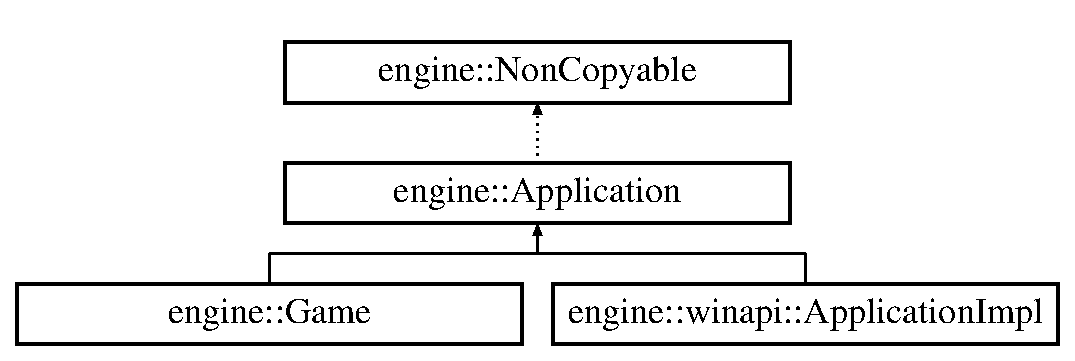
\includegraphics[height=3.000000cm]{a00002}
\end{center}
\end{figure}
\subsubsection*{Public Member Functions}
\begin{DoxyCompactItemize}
\item 
\hyperlink{a00002_a8ba1a5c0ffacfa8c22797d62722f1359}{Application} (std\+::unique\+\_\+ptr$<$ \hyperlink{a00043}{I\+Application\+Parameter} $>$ arguments, std\+::unique\+\_\+ptr$<$ \hyperlink{a00045}{I\+Main} $>$ main)
\item 
virtual \hyperlink{a00002_a02c92008318072312a4f972298c77246}{$\sim$\+Application} ()
\item 
void {\bfseries run} ()\hypertarget{a00002_a6d9c94380f1451664ff6d09c314671c7}{}\label{a00002_a6d9c94380f1451664ff6d09c314671c7}

\item 
void \hyperlink{a00002_a149822f20163e98d41728f4752d7a7f7}{update} ()
\item 
void \hyperlink{a00002_af3ef70b1c3e25be0dbe68c460ec2db98}{render} ()
\item 
bool \hyperlink{a00002_a86f249cf621c4255df1a60987c588961}{is\+Active} () const 
\item 
void \hyperlink{a00002_aeb61beceae055e7681b6791dd5dddafa}{stop} ()
\item 
void \hyperlink{a00002_a9b8b10fd48e93db0986df610523105dc}{start} ()
\item 
const \hyperlink{a00043}{I\+Application\+Parameter} $\ast$ \hyperlink{a00002_af165b483b86469ff9db2f689f1212f14}{get\+Arguments} () const 
\item 
\hyperlink{a00034}{Event\+Manager} $\ast$ {\bfseries get\+Event\+Manager} () const \hypertarget{a00002_aa895c5c2a56efe782cd9cb038075bb60}{}\label{a00002_aa895c5c2a56efe782cd9cb038075bb60}

\item 
\hyperlink{a00087}{Window\+Manager} $\ast$ {\bfseries get\+Window\+Manager} () const \hypertarget{a00002_aed35eca596bce4c089aa3db72d3dc5b6}{}\label{a00002_aed35eca596bce4c089aa3db72d3dc5b6}

\end{DoxyCompactItemize}
\subsubsection*{Friends}
\begin{DoxyCompactItemize}
\item 
class {\bfseries Base\+Builder}\hypertarget{a00002_ad579f1883f887a1593ef8d2161435124}{}\label{a00002_ad579f1883f887a1593ef8d2161435124}

\end{DoxyCompactItemize}


\subsubsection{Detailed Description}
Class for the application main logic. 

Definition at line 21 of file Application.\+h.



\subsubsection{Constructor \& Destructor Documentation}
\index{engine\+::\+Application@{engine\+::\+Application}!Application@{Application}}
\index{Application@{Application}!engine\+::\+Application@{engine\+::\+Application}}
\paragraph[{\texorpdfstring{Application(std\+::unique\+\_\+ptr$<$ I\+Application\+Parameter $>$ arguments, std\+::unique\+\_\+ptr$<$ I\+Main $>$ main)}{Application(std::unique_ptr< IApplicationParameter > arguments, std::unique_ptr< IMain > main)}}]{\setlength{\rightskip}{0pt plus 5cm}engine\+::\+Application\+::\+Application (
\begin{DoxyParamCaption}
\item[{std\+::unique\+\_\+ptr$<$ {\bf I\+Application\+Parameter} $>$}]{arguments, }
\item[{std\+::unique\+\_\+ptr$<$ {\bf I\+Main} $>$}]{main}
\end{DoxyParamCaption}
)}\hypertarget{a00002_a8ba1a5c0ffacfa8c22797d62722f1359}{}\label{a00002_a8ba1a5c0ffacfa8c22797d62722f1359}
Create an application with the given arguments. 
\begin{DoxyParams}{Parameters}
{\em arguments} & \hyperlink{a00002}{Application} arguments, tipically forwarded from tha main function. \\
\hline
{\em main} & \hyperlink{a00002}{Application} core logic. \\
\hline
\end{DoxyParams}
\index{engine\+::\+Application@{engine\+::\+Application}!````~Application@{$\sim$\+Application}}
\index{````~Application@{$\sim$\+Application}!engine\+::\+Application@{engine\+::\+Application}}
\paragraph[{\texorpdfstring{$\sim$\+Application()}{~Application()}}]{\setlength{\rightskip}{0pt plus 5cm}virtual engine\+::\+Application\+::$\sim$\+Application (
\begin{DoxyParamCaption}
{}
\end{DoxyParamCaption}
)\hspace{0.3cm}{\ttfamily [virtual]}}\hypertarget{a00002_a02c92008318072312a4f972298c77246}{}\label{a00002_a02c92008318072312a4f972298c77246}
Simple destructor for P\+I\+M\+PL 

\subsubsection{Member Function Documentation}
\index{engine\+::\+Application@{engine\+::\+Application}!get\+Arguments@{get\+Arguments}}
\index{get\+Arguments@{get\+Arguments}!engine\+::\+Application@{engine\+::\+Application}}
\paragraph[{\texorpdfstring{get\+Arguments() const }{getArguments() const }}]{\setlength{\rightskip}{0pt plus 5cm}const {\bf I\+Application\+Parameter}$\ast$ engine\+::\+Application\+::get\+Arguments (
\begin{DoxyParamCaption}
{}
\end{DoxyParamCaption}
) const}\hypertarget{a00002_af165b483b86469ff9db2f689f1212f14}{}\label{a00002_af165b483b86469ff9db2f689f1212f14}
\begin{DoxyReturn}{Returns}
Returns the initial arguments of the application 
\end{DoxyReturn}
\index{engine\+::\+Application@{engine\+::\+Application}!is\+Active@{is\+Active}}
\index{is\+Active@{is\+Active}!engine\+::\+Application@{engine\+::\+Application}}
\paragraph[{\texorpdfstring{is\+Active() const }{isActive() const }}]{\setlength{\rightskip}{0pt plus 5cm}bool engine\+::\+Application\+::is\+Active (
\begin{DoxyParamCaption}
{}
\end{DoxyParamCaption}
) const}\hypertarget{a00002_a86f249cf621c4255df1a60987c588961}{}\label{a00002_a86f249cf621c4255df1a60987c588961}
\begin{DoxyReturn}{Returns}
Returns true till the application is not terminated. 
\end{DoxyReturn}
\index{engine\+::\+Application@{engine\+::\+Application}!render@{render}}
\index{render@{render}!engine\+::\+Application@{engine\+::\+Application}}
\paragraph[{\texorpdfstring{render()}{render()}}]{\setlength{\rightskip}{0pt plus 5cm}void engine\+::\+Application\+::render (
\begin{DoxyParamCaption}
{}
\end{DoxyParamCaption}
)}\hypertarget{a00002_af3ef70b1c3e25be0dbe68c460ec2db98}{}\label{a00002_af3ef70b1c3e25be0dbe68c460ec2db98}
Render is called in each frame. Here will be rendered the application \index{engine\+::\+Application@{engine\+::\+Application}!start@{start}}
\index{start@{start}!engine\+::\+Application@{engine\+::\+Application}}
\paragraph[{\texorpdfstring{start()}{start()}}]{\setlength{\rightskip}{0pt plus 5cm}void engine\+::\+Application\+::start (
\begin{DoxyParamCaption}
{}
\end{DoxyParamCaption}
)}\hypertarget{a00002_a9b8b10fd48e93db0986df610523105dc}{}\label{a00002_a9b8b10fd48e93db0986df610523105dc}
Terminate the application \index{engine\+::\+Application@{engine\+::\+Application}!stop@{stop}}
\index{stop@{stop}!engine\+::\+Application@{engine\+::\+Application}}
\paragraph[{\texorpdfstring{stop()}{stop()}}]{\setlength{\rightskip}{0pt plus 5cm}void engine\+::\+Application\+::stop (
\begin{DoxyParamCaption}
{}
\end{DoxyParamCaption}
)}\hypertarget{a00002_aeb61beceae055e7681b6791dd5dddafa}{}\label{a00002_aeb61beceae055e7681b6791dd5dddafa}
Starts the application. \index{engine\+::\+Application@{engine\+::\+Application}!update@{update}}
\index{update@{update}!engine\+::\+Application@{engine\+::\+Application}}
\paragraph[{\texorpdfstring{update()}{update()}}]{\setlength{\rightskip}{0pt plus 5cm}void engine\+::\+Application\+::update (
\begin{DoxyParamCaption}
{}
\end{DoxyParamCaption}
)}\hypertarget{a00002_a149822f20163e98d41728f4752d7a7f7}{}\label{a00002_a149822f20163e98d41728f4752d7a7f7}
Update is called once per each frame 

The documentation for this class was generated from the following file\+:\begin{DoxyCompactItemize}
\item 
E\+:/\+Programing/\+Projects/\+Engine\+Workspace/\+Common\+Libs/engine/include/engine/app/Application.\+h\end{DoxyCompactItemize}

\hypertarget{a00003}{}\subsection{engine\+:\+:Application\+Builder Class Reference}
\label{a00003}\index{engine\+::\+Application\+Builder@{engine\+::\+Application\+Builder}}


{\ttfamily \#include $<$E\+:/\+Programing/\+Projects/\+Engine\+Workspace/\+Common\+Libs/engine/include/engine/environment\+Builder/\+Application\+Builder.\+h$>$}

Inheritance diagram for engine\+:\+:Application\+Builder\+:\begin{figure}[H]
\begin{center}
\leavevmode
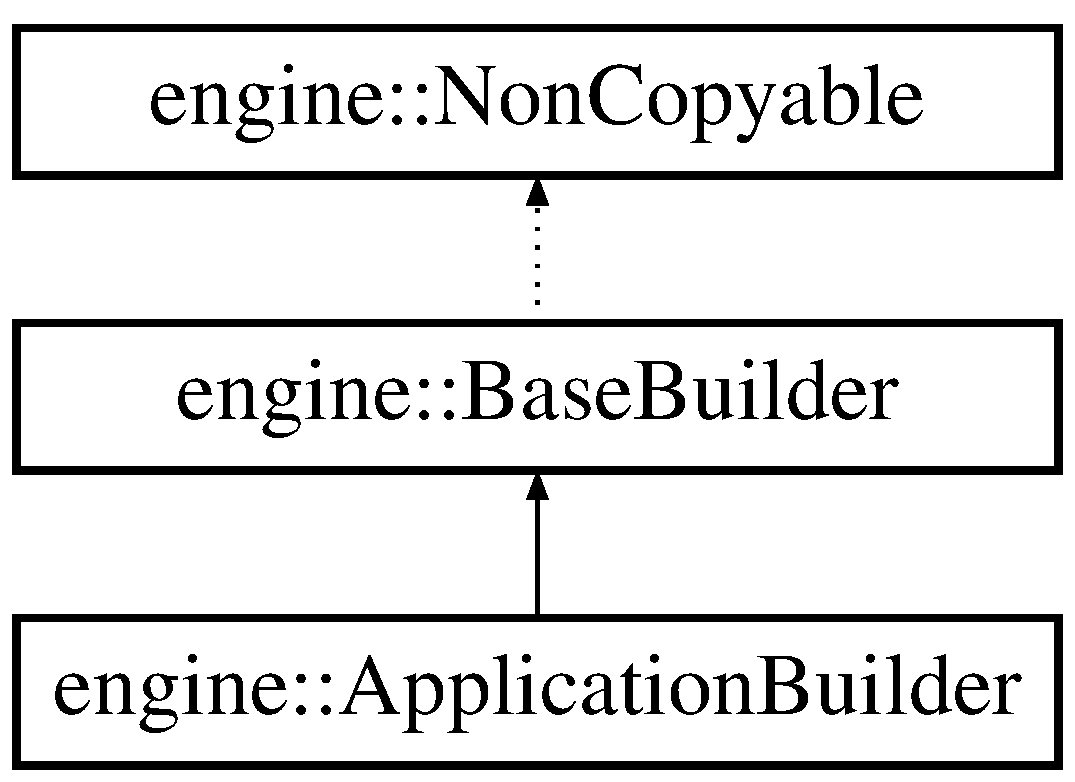
\includegraphics[height=3.000000cm]{a00003}
\end{center}
\end{figure}
\subsubsection*{Public Member Functions}
\begin{DoxyCompactItemize}
\item 
{\bfseries Application\+Builder} (\hyperlink{a00003}{Application\+Builder} \&\&o)\hypertarget{a00003_a9129ac9644ef145a394c99d59c035307}{}\label{a00003_a9129ac9644ef145a394c99d59c035307}

\item 
\hyperlink{a00031}{Event\+Builder} \hyperlink{a00003_a7ca2bdeae296ff836f6592b66d819e87}{build} (std\+::unique\+\_\+ptr$<$ \hyperlink{a00043}{I\+Application\+Parameter} $>$ arguments, std\+::unique\+\_\+ptr$<$ \hyperlink{a00045}{I\+Main} $>$ main)
\end{DoxyCompactItemize}
\subsubsection*{Protected Member Functions}
\begin{DoxyCompactItemize}
\item 
void \hyperlink{a00005_a52fb449fadc5d3a074e3fc7bfb56744b}{add\+Module} (const Context\+Module\+Type value)
\item 
void \hyperlink{a00005_a20c5dafa6892142bc352c13a5f3ac09a}{set\+Application} (std\+::unique\+\_\+ptr$<$ \hyperlink{a00002}{Application} $>$ app)
\item 
void \hyperlink{a00005_a641fb06484bdb07220f445f14db8c0e7}{set\+Window\+Manager} (std\+::unique\+\_\+ptr$<$ \hyperlink{a00087}{Window\+Manager} $>$ manager)
\item 
void \hyperlink{a00005_a52b490a3ef4d2a5b5b7e8e0f82d9a27c}{set\+Event\+Manager} (std\+::unique\+\_\+ptr$<$ \hyperlink{a00034}{Event\+Manager} $>$ manager)
\item 
void \hyperlink{a00005_af23e3bdfb30ca9f2076cacc9029d96c2}{set\+Initialized} ()
\end{DoxyCompactItemize}
\subsubsection*{Friends}
\begin{DoxyCompactItemize}
\item 
class {\bfseries Context\+Builder}\hypertarget{a00003_a528d730eed168c7dd3a6f53bce42cbcf}{}\label{a00003_a528d730eed168c7dd3a6f53bce42cbcf}

\end{DoxyCompactItemize}


\subsubsection{Detailed Description}
This is the application building phase. After this build phase the context will have an application 

Definition at line 21 of file Application\+Builder.\+h.



\subsubsection{Member Function Documentation}
\index{engine\+::\+Application\+Builder@{engine\+::\+Application\+Builder}!add\+Module@{add\+Module}}
\index{add\+Module@{add\+Module}!engine\+::\+Application\+Builder@{engine\+::\+Application\+Builder}}
\paragraph[{\texorpdfstring{add\+Module(const Context\+Module\+Type value)}{addModule(const ContextModuleType value)}}]{\setlength{\rightskip}{0pt plus 5cm}void engine\+::\+Base\+Builder\+::add\+Module (
\begin{DoxyParamCaption}
\item[{const Context\+Module\+Type}]{value}
\end{DoxyParamCaption}
)\hspace{0.3cm}{\ttfamily [protected]}, {\ttfamily [inherited]}}\hypertarget{a00005_a52fb449fadc5d3a074e3fc7bfb56744b}{}\label{a00005_a52fb449fadc5d3a074e3fc7bfb56744b}
Add a module type which is initialized during build phase 
\begin{DoxyParams}{Parameters}
{\em value} & Module which is initialized successfully \\
\hline
\end{DoxyParams}


Referenced by engine\+::\+Base\+Builder\+::$\sim$\+Base\+Builder().

\index{engine\+::\+Application\+Builder@{engine\+::\+Application\+Builder}!build@{build}}
\index{build@{build}!engine\+::\+Application\+Builder@{engine\+::\+Application\+Builder}}
\paragraph[{\texorpdfstring{build(std\+::unique\+\_\+ptr$<$ I\+Application\+Parameter $>$ arguments, std\+::unique\+\_\+ptr$<$ I\+Main $>$ main)}{build(std::unique_ptr< IApplicationParameter > arguments, std::unique_ptr< IMain > main)}}]{\setlength{\rightskip}{0pt plus 5cm}{\bf Event\+Builder} engine\+::\+Application\+Builder\+::build (
\begin{DoxyParamCaption}
\item[{std\+::unique\+\_\+ptr$<$ {\bf I\+Application\+Parameter} $>$}]{arguments, }
\item[{std\+::unique\+\_\+ptr$<$ {\bf I\+Main} $>$}]{main}
\end{DoxyParamCaption}
)}\hypertarget{a00003_a7ca2bdeae296ff836f6592b66d819e87}{}\label{a00003_a7ca2bdeae296ff836f6592b66d819e87}
Build an application with the given arguments and main. 
\begin{DoxyParams}{Parameters}
{\em arguments} & arguments of the application \\
\hline
{\em main} & Main functionality. \\
\hline
\end{DoxyParams}
\begin{DoxyReturn}{Returns}
The next building phase. 
\end{DoxyReturn}
\index{engine\+::\+Application\+Builder@{engine\+::\+Application\+Builder}!set\+Application@{set\+Application}}
\index{set\+Application@{set\+Application}!engine\+::\+Application\+Builder@{engine\+::\+Application\+Builder}}
\paragraph[{\texorpdfstring{set\+Application(std\+::unique\+\_\+ptr$<$ Application $>$ app)}{setApplication(std::unique_ptr< Application > app)}}]{\setlength{\rightskip}{0pt plus 5cm}void engine\+::\+Base\+Builder\+::set\+Application (
\begin{DoxyParamCaption}
\item[{std\+::unique\+\_\+ptr$<$ {\bf Application} $>$}]{app}
\end{DoxyParamCaption}
)\hspace{0.3cm}{\ttfamily [protected]}, {\ttfamily [inherited]}}\hypertarget{a00005_a20c5dafa6892142bc352c13a5f3ac09a}{}\label{a00005_a20c5dafa6892142bc352c13a5f3ac09a}
Set the context application. 
\begin{DoxyParams}{Parameters}
{\em app} & \hyperlink{a00002}{Application} to use \\
\hline
\end{DoxyParams}


Referenced by engine\+::\+Base\+Builder\+::$\sim$\+Base\+Builder().

\index{engine\+::\+Application\+Builder@{engine\+::\+Application\+Builder}!set\+Event\+Manager@{set\+Event\+Manager}}
\index{set\+Event\+Manager@{set\+Event\+Manager}!engine\+::\+Application\+Builder@{engine\+::\+Application\+Builder}}
\paragraph[{\texorpdfstring{set\+Event\+Manager(std\+::unique\+\_\+ptr$<$ Event\+Manager $>$ manager)}{setEventManager(std::unique_ptr< EventManager > manager)}}]{\setlength{\rightskip}{0pt plus 5cm}void engine\+::\+Base\+Builder\+::set\+Event\+Manager (
\begin{DoxyParamCaption}
\item[{std\+::unique\+\_\+ptr$<$ {\bf Event\+Manager} $>$}]{manager}
\end{DoxyParamCaption}
)\hspace{0.3cm}{\ttfamily [protected]}, {\ttfamily [inherited]}}\hypertarget{a00005_a52b490a3ef4d2a5b5b7e8e0f82d9a27c}{}\label{a00005_a52b490a3ef4d2a5b5b7e8e0f82d9a27c}
Set the event manager of the context. 
\begin{DoxyParams}{Parameters}
{\em manager} & window manager to use \\
\hline
\end{DoxyParams}


Referenced by engine\+::\+Base\+Builder\+::$\sim$\+Base\+Builder().

\index{engine\+::\+Application\+Builder@{engine\+::\+Application\+Builder}!set\+Initialized@{set\+Initialized}}
\index{set\+Initialized@{set\+Initialized}!engine\+::\+Application\+Builder@{engine\+::\+Application\+Builder}}
\paragraph[{\texorpdfstring{set\+Initialized()}{setInitialized()}}]{\setlength{\rightskip}{0pt plus 5cm}void engine\+::\+Base\+Builder\+::set\+Initialized (
\begin{DoxyParamCaption}
{}
\end{DoxyParamCaption}
)\hspace{0.3cm}{\ttfamily [protected]}, {\ttfamily [inherited]}}\hypertarget{a00005_af23e3bdfb30ca9f2076cacc9029d96c2}{}\label{a00005_af23e3bdfb30ca9f2076cacc9029d96c2}
When the environment is built up this function finalize the context. 

Referenced by engine\+::\+Base\+Builder\+::$\sim$\+Base\+Builder().

\index{engine\+::\+Application\+Builder@{engine\+::\+Application\+Builder}!set\+Window\+Manager@{set\+Window\+Manager}}
\index{set\+Window\+Manager@{set\+Window\+Manager}!engine\+::\+Application\+Builder@{engine\+::\+Application\+Builder}}
\paragraph[{\texorpdfstring{set\+Window\+Manager(std\+::unique\+\_\+ptr$<$ Window\+Manager $>$ manager)}{setWindowManager(std::unique_ptr< WindowManager > manager)}}]{\setlength{\rightskip}{0pt plus 5cm}void engine\+::\+Base\+Builder\+::set\+Window\+Manager (
\begin{DoxyParamCaption}
\item[{std\+::unique\+\_\+ptr$<$ {\bf Window\+Manager} $>$}]{manager}
\end{DoxyParamCaption}
)\hspace{0.3cm}{\ttfamily [protected]}, {\ttfamily [inherited]}}\hypertarget{a00005_a641fb06484bdb07220f445f14db8c0e7}{}\label{a00005_a641fb06484bdb07220f445f14db8c0e7}
Set the window manager of the context. 
\begin{DoxyParams}{Parameters}
{\em manager} & window manager to use \\
\hline
\end{DoxyParams}


Referenced by engine\+::\+Base\+Builder\+::$\sim$\+Base\+Builder().



The documentation for this class was generated from the following file\+:\begin{DoxyCompactItemize}
\item 
E\+:/\+Programing/\+Projects/\+Engine\+Workspace/\+Common\+Libs/engine/include/engine/environment\+Builder/Application\+Builder.\+h\end{DoxyCompactItemize}

\hypertarget{a00004}{}\subsection{engine\+:\+:winapi\+:\+:Application\+Impl Class Reference}
\label{a00004}\index{engine\+::winapi\+::\+Application\+Impl@{engine\+::winapi\+::\+Application\+Impl}}
Inheritance diagram for engine\+:\+:winapi\+:\+:Application\+Impl\+:\begin{figure}[H]
\begin{center}
\leavevmode
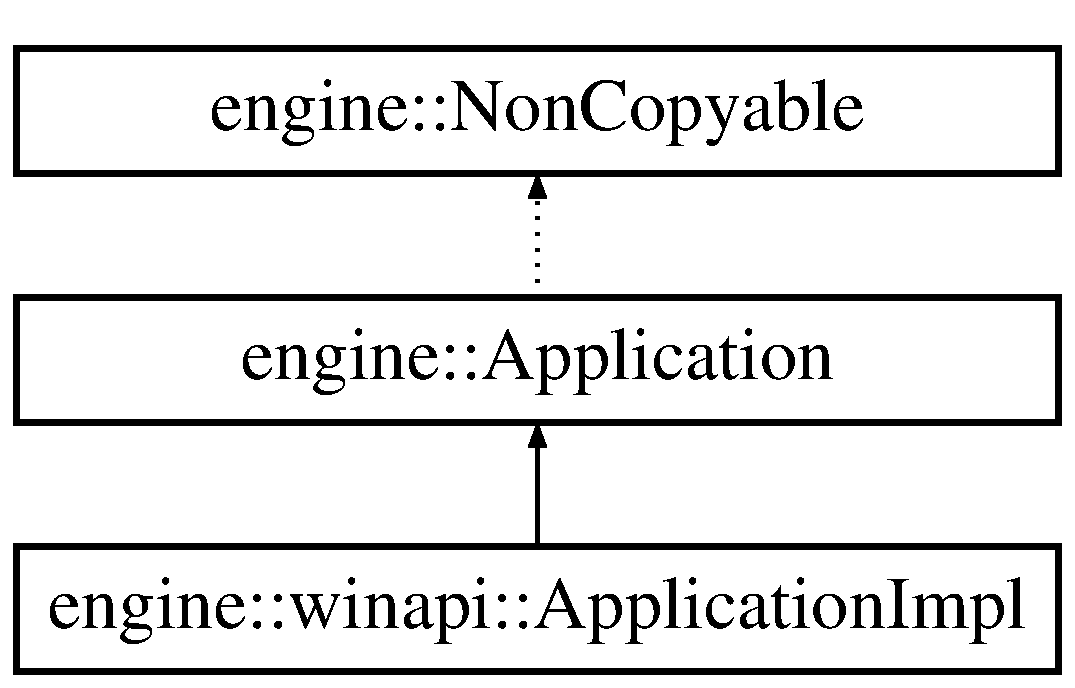
\includegraphics[height=3.000000cm]{a00004}
\end{center}
\end{figure}
\subsubsection*{Public Member Functions}
\begin{DoxyCompactItemize}
\item 
{\bfseries Application\+Impl} (std\+::unique\+\_\+ptr$<$ \hyperlink{a00043}{I\+Application\+Parameter} $>$ arguments, std\+::unique\+\_\+ptr$<$ \hyperlink{a00045}{I\+Main} $>$ main)\hypertarget{a00004_aae13a8664b4d94cf5a625eb526662599}{}\label{a00004_aae13a8664b4d94cf5a625eb526662599}

\item 
bool {\bfseries handle\+Event} (H\+W\+ND h\+Wnd, U\+I\+NT message, W\+P\+A\+R\+AM w\+Param, L\+P\+A\+R\+AM l\+Param)\hypertarget{a00004_a8622725348cb094eae90294be4896f66}{}\label{a00004_a8622725348cb094eae90294be4896f66}

\item 
void {\bfseries run} ()\hypertarget{a00002_a6d9c94380f1451664ff6d09c314671c7}{}\label{a00002_a6d9c94380f1451664ff6d09c314671c7}

\item 
void \hyperlink{a00002_a149822f20163e98d41728f4752d7a7f7}{update} ()
\item 
void \hyperlink{a00002_af3ef70b1c3e25be0dbe68c460ec2db98}{render} ()
\item 
bool \hyperlink{a00002_a86f249cf621c4255df1a60987c588961}{is\+Active} () const 
\item 
void \hyperlink{a00002_aeb61beceae055e7681b6791dd5dddafa}{stop} ()
\item 
void \hyperlink{a00002_a9b8b10fd48e93db0986df610523105dc}{start} ()
\item 
const \hyperlink{a00043}{I\+Application\+Parameter} $\ast$ \hyperlink{a00002_af165b483b86469ff9db2f689f1212f14}{get\+Arguments} () const 
\item 
\hyperlink{a00034}{Event\+Manager} $\ast$ {\bfseries get\+Event\+Manager} () const \hypertarget{a00002_aa895c5c2a56efe782cd9cb038075bb60}{}\label{a00002_aa895c5c2a56efe782cd9cb038075bb60}

\item 
\hyperlink{a00087}{Window\+Manager} $\ast$ {\bfseries get\+Window\+Manager} () const \hypertarget{a00002_aed35eca596bce4c089aa3db72d3dc5b6}{}\label{a00002_aed35eca596bce4c089aa3db72d3dc5b6}

\end{DoxyCompactItemize}


\subsubsection{Detailed Description}


Definition at line 12 of file Application\+Impl.\+h.



\subsubsection{Member Function Documentation}
\index{engine\+::winapi\+::\+Application\+Impl@{engine\+::winapi\+::\+Application\+Impl}!get\+Arguments@{get\+Arguments}}
\index{get\+Arguments@{get\+Arguments}!engine\+::winapi\+::\+Application\+Impl@{engine\+::winapi\+::\+Application\+Impl}}
\paragraph[{\texorpdfstring{get\+Arguments() const }{getArguments() const }}]{\setlength{\rightskip}{0pt plus 5cm}const {\bf I\+Application\+Parameter}$\ast$ engine\+::\+Application\+::get\+Arguments (
\begin{DoxyParamCaption}
{}
\end{DoxyParamCaption}
) const\hspace{0.3cm}{\ttfamily [inherited]}}\hypertarget{a00002_af165b483b86469ff9db2f689f1212f14}{}\label{a00002_af165b483b86469ff9db2f689f1212f14}
\begin{DoxyReturn}{Returns}
Returns the initial arguments of the application 
\end{DoxyReturn}
\index{engine\+::winapi\+::\+Application\+Impl@{engine\+::winapi\+::\+Application\+Impl}!is\+Active@{is\+Active}}
\index{is\+Active@{is\+Active}!engine\+::winapi\+::\+Application\+Impl@{engine\+::winapi\+::\+Application\+Impl}}
\paragraph[{\texorpdfstring{is\+Active() const }{isActive() const }}]{\setlength{\rightskip}{0pt plus 5cm}bool engine\+::\+Application\+::is\+Active (
\begin{DoxyParamCaption}
{}
\end{DoxyParamCaption}
) const\hspace{0.3cm}{\ttfamily [inherited]}}\hypertarget{a00002_a86f249cf621c4255df1a60987c588961}{}\label{a00002_a86f249cf621c4255df1a60987c588961}
\begin{DoxyReturn}{Returns}
Returns true till the application is not terminated. 
\end{DoxyReturn}
\index{engine\+::winapi\+::\+Application\+Impl@{engine\+::winapi\+::\+Application\+Impl}!render@{render}}
\index{render@{render}!engine\+::winapi\+::\+Application\+Impl@{engine\+::winapi\+::\+Application\+Impl}}
\paragraph[{\texorpdfstring{render()}{render()}}]{\setlength{\rightskip}{0pt plus 5cm}void engine\+::\+Application\+::render (
\begin{DoxyParamCaption}
{}
\end{DoxyParamCaption}
)\hspace{0.3cm}{\ttfamily [inherited]}}\hypertarget{a00002_af3ef70b1c3e25be0dbe68c460ec2db98}{}\label{a00002_af3ef70b1c3e25be0dbe68c460ec2db98}
Render is called in each frame. Here will be rendered the application \index{engine\+::winapi\+::\+Application\+Impl@{engine\+::winapi\+::\+Application\+Impl}!start@{start}}
\index{start@{start}!engine\+::winapi\+::\+Application\+Impl@{engine\+::winapi\+::\+Application\+Impl}}
\paragraph[{\texorpdfstring{start()}{start()}}]{\setlength{\rightskip}{0pt plus 5cm}void engine\+::\+Application\+::start (
\begin{DoxyParamCaption}
{}
\end{DoxyParamCaption}
)\hspace{0.3cm}{\ttfamily [inherited]}}\hypertarget{a00002_a9b8b10fd48e93db0986df610523105dc}{}\label{a00002_a9b8b10fd48e93db0986df610523105dc}
Terminate the application \index{engine\+::winapi\+::\+Application\+Impl@{engine\+::winapi\+::\+Application\+Impl}!stop@{stop}}
\index{stop@{stop}!engine\+::winapi\+::\+Application\+Impl@{engine\+::winapi\+::\+Application\+Impl}}
\paragraph[{\texorpdfstring{stop()}{stop()}}]{\setlength{\rightskip}{0pt plus 5cm}void engine\+::\+Application\+::stop (
\begin{DoxyParamCaption}
{}
\end{DoxyParamCaption}
)\hspace{0.3cm}{\ttfamily [inherited]}}\hypertarget{a00002_aeb61beceae055e7681b6791dd5dddafa}{}\label{a00002_aeb61beceae055e7681b6791dd5dddafa}
Starts the application. \index{engine\+::winapi\+::\+Application\+Impl@{engine\+::winapi\+::\+Application\+Impl}!update@{update}}
\index{update@{update}!engine\+::winapi\+::\+Application\+Impl@{engine\+::winapi\+::\+Application\+Impl}}
\paragraph[{\texorpdfstring{update()}{update()}}]{\setlength{\rightskip}{0pt plus 5cm}void engine\+::\+Application\+::update (
\begin{DoxyParamCaption}
{}
\end{DoxyParamCaption}
)\hspace{0.3cm}{\ttfamily [inherited]}}\hypertarget{a00002_a149822f20163e98d41728f4752d7a7f7}{}\label{a00002_a149822f20163e98d41728f4752d7a7f7}
Update is called once per each frame 

The documentation for this class was generated from the following file\+:\begin{DoxyCompactItemize}
\item 
E\+:/\+Programing/\+Projects/\+Engine\+Workspace/\+Common\+Libs/engine/include/engine/app/winapi/Application\+Impl.\+h\end{DoxyCompactItemize}

\hypertarget{a00005}{}\subsection{engine\+:\+:Base\+Builder Class Reference}
\label{a00005}\index{engine\+::\+Base\+Builder@{engine\+::\+Base\+Builder}}


{\ttfamily \#include $<$E\+:/\+Programing/\+Projects/\+Engine\+Workspace/\+Common\+Libs/engine/include/engine/environment\+Builder/\+Base\+Builder.\+h$>$}

Inheritance diagram for engine\+:\+:Base\+Builder\+:\begin{figure}[H]
\begin{center}
\leavevmode
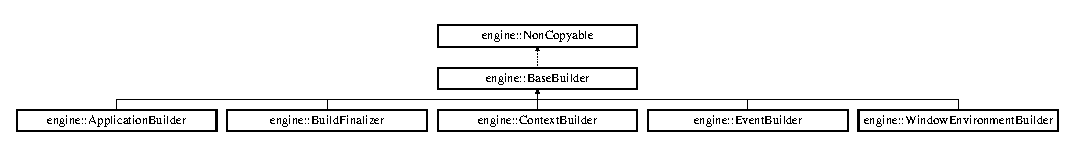
\includegraphics[height=1.541284cm]{a00005}
\end{center}
\end{figure}
\subsubsection*{Protected Member Functions}
\begin{DoxyCompactItemize}
\item 
\hyperlink{a00005_ac1d22d4031be98e715d8ea733fc4463b}{Base\+Builder} ()=default
\item 
virtual \hyperlink{a00005_af762f3acae53396e0621113e1bb3156b}{$\sim$\+Base\+Builder} ()
\item 
void \hyperlink{a00005_a52fb449fadc5d3a074e3fc7bfb56744b}{add\+Module} (const Context\+Module\+Type value)
\item 
void \hyperlink{a00005_a20c5dafa6892142bc352c13a5f3ac09a}{set\+Application} (std\+::unique\+\_\+ptr$<$ \hyperlink{a00002}{Application} $>$ app)
\item 
void \hyperlink{a00005_a641fb06484bdb07220f445f14db8c0e7}{set\+Window\+Manager} (std\+::unique\+\_\+ptr$<$ \hyperlink{a00087}{Window\+Manager} $>$ manager)
\item 
void \hyperlink{a00005_a52b490a3ef4d2a5b5b7e8e0f82d9a27c}{set\+Event\+Manager} (std\+::unique\+\_\+ptr$<$ \hyperlink{a00034}{Event\+Manager} $>$ manager)
\item 
void \hyperlink{a00005_af23e3bdfb30ca9f2076cacc9029d96c2}{set\+Initialized} ()
\end{DoxyCompactItemize}


\subsubsection{Detailed Description}
Base class for builder phases. Only via this class one can set up context parameters. 

Definition at line 20 of file Base\+Builder.\+h.



\subsubsection{Constructor \& Destructor Documentation}
\index{engine\+::\+Base\+Builder@{engine\+::\+Base\+Builder}!Base\+Builder@{Base\+Builder}}
\index{Base\+Builder@{Base\+Builder}!engine\+::\+Base\+Builder@{engine\+::\+Base\+Builder}}
\paragraph[{\texorpdfstring{Base\+Builder()=default}{BaseBuilder()=default}}]{\setlength{\rightskip}{0pt plus 5cm}engine\+::\+Base\+Builder\+::\+Base\+Builder (
\begin{DoxyParamCaption}
{}
\end{DoxyParamCaption}
)\hspace{0.3cm}{\ttfamily [protected]}, {\ttfamily [default]}}\hypertarget{a00005_ac1d22d4031be98e715d8ea733fc4463b}{}\label{a00005_ac1d22d4031be98e715d8ea733fc4463b}
Default constructor \index{engine\+::\+Base\+Builder@{engine\+::\+Base\+Builder}!````~Base\+Builder@{$\sim$\+Base\+Builder}}
\index{````~Base\+Builder@{$\sim$\+Base\+Builder}!engine\+::\+Base\+Builder@{engine\+::\+Base\+Builder}}
\paragraph[{\texorpdfstring{$\sim$\+Base\+Builder()}{~BaseBuilder()}}]{\setlength{\rightskip}{0pt plus 5cm}virtual engine\+::\+Base\+Builder\+::$\sim$\+Base\+Builder (
\begin{DoxyParamCaption}
{}
\end{DoxyParamCaption}
)\hspace{0.3cm}{\ttfamily [inline]}, {\ttfamily [protected]}, {\ttfamily [virtual]}}\hypertarget{a00005_af762f3acae53396e0621113e1bb3156b}{}\label{a00005_af762f3acae53396e0621113e1bb3156b}
Default destructor 

Definition at line 26 of file Base\+Builder.\+h.



\subsubsection{Member Function Documentation}
\index{engine\+::\+Base\+Builder@{engine\+::\+Base\+Builder}!add\+Module@{add\+Module}}
\index{add\+Module@{add\+Module}!engine\+::\+Base\+Builder@{engine\+::\+Base\+Builder}}
\paragraph[{\texorpdfstring{add\+Module(const Context\+Module\+Type value)}{addModule(const ContextModuleType value)}}]{\setlength{\rightskip}{0pt plus 5cm}void engine\+::\+Base\+Builder\+::add\+Module (
\begin{DoxyParamCaption}
\item[{const Context\+Module\+Type}]{value}
\end{DoxyParamCaption}
)\hspace{0.3cm}{\ttfamily [protected]}}\hypertarget{a00005_a52fb449fadc5d3a074e3fc7bfb56744b}{}\label{a00005_a52fb449fadc5d3a074e3fc7bfb56744b}
Add a module type which is initialized during build phase 
\begin{DoxyParams}{Parameters}
{\em value} & Module which is initialized successfully \\
\hline
\end{DoxyParams}


Referenced by $\sim$\+Base\+Builder().

\index{engine\+::\+Base\+Builder@{engine\+::\+Base\+Builder}!set\+Application@{set\+Application}}
\index{set\+Application@{set\+Application}!engine\+::\+Base\+Builder@{engine\+::\+Base\+Builder}}
\paragraph[{\texorpdfstring{set\+Application(std\+::unique\+\_\+ptr$<$ Application $>$ app)}{setApplication(std::unique_ptr< Application > app)}}]{\setlength{\rightskip}{0pt plus 5cm}void engine\+::\+Base\+Builder\+::set\+Application (
\begin{DoxyParamCaption}
\item[{std\+::unique\+\_\+ptr$<$ {\bf Application} $>$}]{app}
\end{DoxyParamCaption}
)\hspace{0.3cm}{\ttfamily [protected]}}\hypertarget{a00005_a20c5dafa6892142bc352c13a5f3ac09a}{}\label{a00005_a20c5dafa6892142bc352c13a5f3ac09a}
Set the context application. 
\begin{DoxyParams}{Parameters}
{\em app} & \hyperlink{a00002}{Application} to use \\
\hline
\end{DoxyParams}


Referenced by $\sim$\+Base\+Builder().

\index{engine\+::\+Base\+Builder@{engine\+::\+Base\+Builder}!set\+Event\+Manager@{set\+Event\+Manager}}
\index{set\+Event\+Manager@{set\+Event\+Manager}!engine\+::\+Base\+Builder@{engine\+::\+Base\+Builder}}
\paragraph[{\texorpdfstring{set\+Event\+Manager(std\+::unique\+\_\+ptr$<$ Event\+Manager $>$ manager)}{setEventManager(std::unique_ptr< EventManager > manager)}}]{\setlength{\rightskip}{0pt plus 5cm}void engine\+::\+Base\+Builder\+::set\+Event\+Manager (
\begin{DoxyParamCaption}
\item[{std\+::unique\+\_\+ptr$<$ {\bf Event\+Manager} $>$}]{manager}
\end{DoxyParamCaption}
)\hspace{0.3cm}{\ttfamily [protected]}}\hypertarget{a00005_a52b490a3ef4d2a5b5b7e8e0f82d9a27c}{}\label{a00005_a52b490a3ef4d2a5b5b7e8e0f82d9a27c}
Set the event manager of the context. 
\begin{DoxyParams}{Parameters}
{\em manager} & window manager to use \\
\hline
\end{DoxyParams}


Referenced by $\sim$\+Base\+Builder().

\index{engine\+::\+Base\+Builder@{engine\+::\+Base\+Builder}!set\+Initialized@{set\+Initialized}}
\index{set\+Initialized@{set\+Initialized}!engine\+::\+Base\+Builder@{engine\+::\+Base\+Builder}}
\paragraph[{\texorpdfstring{set\+Initialized()}{setInitialized()}}]{\setlength{\rightskip}{0pt plus 5cm}void engine\+::\+Base\+Builder\+::set\+Initialized (
\begin{DoxyParamCaption}
{}
\end{DoxyParamCaption}
)\hspace{0.3cm}{\ttfamily [protected]}}\hypertarget{a00005_af23e3bdfb30ca9f2076cacc9029d96c2}{}\label{a00005_af23e3bdfb30ca9f2076cacc9029d96c2}
When the environment is built up this function finalize the context. 

Referenced by $\sim$\+Base\+Builder().

\index{engine\+::\+Base\+Builder@{engine\+::\+Base\+Builder}!set\+Window\+Manager@{set\+Window\+Manager}}
\index{set\+Window\+Manager@{set\+Window\+Manager}!engine\+::\+Base\+Builder@{engine\+::\+Base\+Builder}}
\paragraph[{\texorpdfstring{set\+Window\+Manager(std\+::unique\+\_\+ptr$<$ Window\+Manager $>$ manager)}{setWindowManager(std::unique_ptr< WindowManager > manager)}}]{\setlength{\rightskip}{0pt plus 5cm}void engine\+::\+Base\+Builder\+::set\+Window\+Manager (
\begin{DoxyParamCaption}
\item[{std\+::unique\+\_\+ptr$<$ {\bf Window\+Manager} $>$}]{manager}
\end{DoxyParamCaption}
)\hspace{0.3cm}{\ttfamily [protected]}}\hypertarget{a00005_a641fb06484bdb07220f445f14db8c0e7}{}\label{a00005_a641fb06484bdb07220f445f14db8c0e7}
Set the window manager of the context. 
\begin{DoxyParams}{Parameters}
{\em manager} & window manager to use \\
\hline
\end{DoxyParams}


Referenced by $\sim$\+Base\+Builder().



The documentation for this class was generated from the following file\+:\begin{DoxyCompactItemize}
\item 
E\+:/\+Programing/\+Projects/\+Engine\+Workspace/\+Common\+Libs/engine/include/engine/environment\+Builder/Base\+Builder.\+h\end{DoxyCompactItemize}

\hypertarget{a00006}{}\subsection{engine\+:\+:test\+:\+:Base\+Regression Class Reference}
\label{a00006}\index{engine\+::test\+::\+Base\+Regression@{engine\+::test\+::\+Base\+Regression}}
Inheritance diagram for engine\+:\+:test\+:\+:Base\+Regression\+:\begin{figure}[H]
\begin{center}
\leavevmode
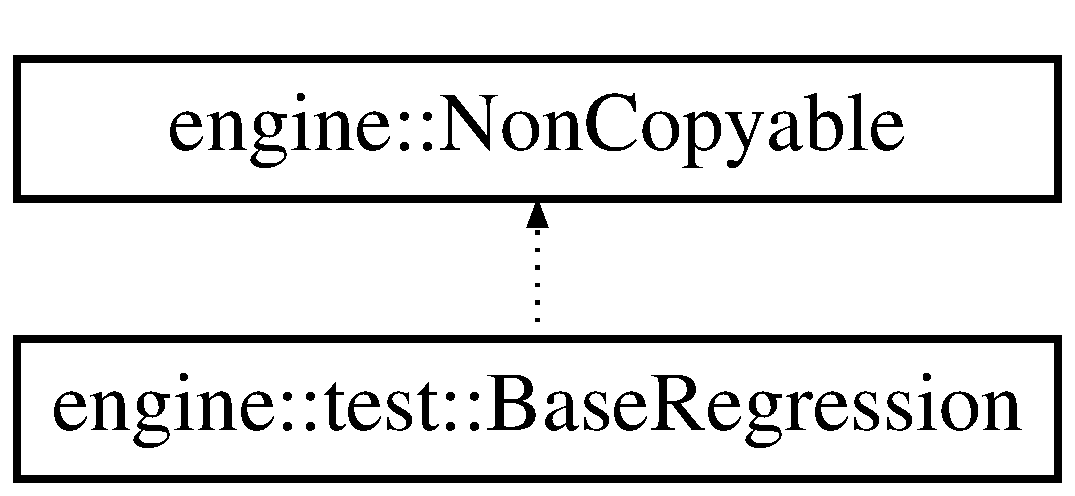
\includegraphics[height=2.000000cm]{a00006}
\end{center}
\end{figure}
\subsubsection*{Public Member Functions}
\begin{DoxyCompactItemize}
\item 
{\bfseries Base\+Regression} (const std\+::string \&name)\hypertarget{a00006_a8fabc03796870f6fc5f7268ce178ce3b}{}\label{a00006_a8fabc03796870f6fc5f7268ce178ce3b}

\item 
{\bfseries Base\+Regression} (\hyperlink{a00006}{Base\+Regression} \&\&o)\hypertarget{a00006_a5649c6763dc88ff4073f27bdc2f718a0}{}\label{a00006_a5649c6763dc88ff4073f27bdc2f718a0}

\item 
void {\bfseries set\+Stream} (std\+::ostream $\ast$os)\hypertarget{a00006_a13f0523e2c149436b9df0ac387d832cf}{}\label{a00006_a13f0523e2c149436b9df0ac387d832cf}

\item 
void {\bfseries run} () const \hypertarget{a00006_a796b6b12ced0f2e5972b9cd249321f22}{}\label{a00006_a796b6b12ced0f2e5972b9cd249321f22}

\item 
uint32\+\_\+t {\bfseries get\+Num\+Of\+Executed\+TC} () const \hypertarget{a00006_afe9eac73f67f52b7c1fbbb137d4c9092}{}\label{a00006_afe9eac73f67f52b7c1fbbb137d4c9092}

\item 
uint32\+\_\+t {\bfseries get\+Num\+Of\+Nok\+TC} () const \hypertarget{a00006_a07c85b15a052a380ebdbcb934f6368a1}{}\label{a00006_a07c85b15a052a380ebdbcb934f6368a1}

\item 
const std\+::string \& {\bfseries get\+Name} () const \hypertarget{a00006_ad4cc8d1ae709af2acd37463f9d378a77}{}\label{a00006_ad4cc8d1ae709af2acd37463f9d378a77}

\end{DoxyCompactItemize}
\subsubsection*{Protected Member Functions}
\begin{DoxyCompactItemize}
\item 
void {\bfseries add\+Test\+Suite} (std\+::unique\+\_\+ptr$<$ \hyperlink{a00077}{Test\+Suite} $>$ \&\&test\+Suite)\hypertarget{a00006_a06d2d89b7427837020675fef014d5545}{}\label{a00006_a06d2d89b7427837020675fef014d5545}

\end{DoxyCompactItemize}


\subsubsection{Detailed Description}


Definition at line 11 of file Base\+Regression.\+h.



The documentation for this class was generated from the following file\+:\begin{DoxyCompactItemize}
\item 
E\+:/\+Programing/\+Projects/\+Engine\+Workspace/\+Common\+Libs/engine/include/engine/test/Base\+Regression.\+h\end{DoxyCompactItemize}

\hypertarget{a00007}{}\subsection{engine\+:\+:Buffer\+Desc Struct Reference}
\label{a00007}\index{engine\+::\+Buffer\+Desc@{engine\+::\+Buffer\+Desc}}


{\ttfamily \#include $<$E\+:/\+Programing/\+Projects/\+Engine\+Workspace/\+Common\+Libs/engine/include/engine/video/\+Buffer\+Desc.\+h$>$}

\subsubsection*{Public Attributes}
\begin{DoxyCompactItemize}
\item 
Texture\+Format \hyperlink{a00007_a5a84b0faa10bdbcd51ddb3936295d82c}{format} = Texture\+Format\+::\+\_\+\+Unknown
\item 
Buffer\+Type \hyperlink{a00007_aaac2389a71fd61b51cd539da66fbc240}{type} = Buffer\+Type\+::\+Undef
\item 
bool \hyperlink{a00007_a50a45012458646eb58890de16c6f5fae}{is\+S\+R\+GB} = false
\item 
Buffer\+Format \hyperlink{a00007_a99d4db16d6b3d3bbb5da5ac64610bb3a}{format} = Buffer\+Format\+::\+Format\+\_\+\+Unknown
\end{DoxyCompactItemize}


\subsubsection{Detailed Description}
Buffer descriptor 

Definition at line 82 of file Buffer\+Desc.\+h.



\subsubsection{Member Data Documentation}
\index{engine\+::\+Buffer\+Desc@{engine\+::\+Buffer\+Desc}!format@{format}}
\index{format@{format}!engine\+::\+Buffer\+Desc@{engine\+::\+Buffer\+Desc}}
\paragraph[{\texorpdfstring{format}{format}}]{\setlength{\rightskip}{0pt plus 5cm}Texture\+Format engine\+::\+Buffer\+Desc\+::format = Texture\+Format\+::\+\_\+\+Unknown}\hypertarget{a00007_a5a84b0faa10bdbcd51ddb3936295d82c}{}\label{a00007_a5a84b0faa10bdbcd51ddb3936295d82c}
Format of the buffer 

Definition at line 85 of file Buffer\+Desc.\+h.

\index{engine\+::\+Buffer\+Desc@{engine\+::\+Buffer\+Desc}!format@{format}}
\index{format@{format}!engine\+::\+Buffer\+Desc@{engine\+::\+Buffer\+Desc}}
\paragraph[{\texorpdfstring{format}{format}}]{\setlength{\rightskip}{0pt plus 5cm}Buffer\+Format engine\+::\+Buffer\+Desc\+::format = Buffer\+Format\+::\+Format\+\_\+\+Unknown}\hypertarget{a00007_a99d4db16d6b3d3bbb5da5ac64610bb3a}{}\label{a00007_a99d4db16d6b3d3bbb5da5ac64610bb3a}
Format of the buffer 

Definition at line 85 of file Buffer\+Desc.\+h.

\index{engine\+::\+Buffer\+Desc@{engine\+::\+Buffer\+Desc}!is\+S\+R\+GB@{is\+S\+R\+GB}}
\index{is\+S\+R\+GB@{is\+S\+R\+GB}!engine\+::\+Buffer\+Desc@{engine\+::\+Buffer\+Desc}}
\paragraph[{\texorpdfstring{is\+S\+R\+GB}{isSRGB}}]{\setlength{\rightskip}{0pt plus 5cm}bool engine\+::\+Buffer\+Desc\+::is\+S\+R\+GB = false}\hypertarget{a00007_a50a45012458646eb58890de16c6f5fae}{}\label{a00007_a50a45012458646eb58890de16c6f5fae}
True if it is an S\+R\+GB buffer 

Definition at line 89 of file Buffer\+Desc.\+h.

\index{engine\+::\+Buffer\+Desc@{engine\+::\+Buffer\+Desc}!type@{type}}
\index{type@{type}!engine\+::\+Buffer\+Desc@{engine\+::\+Buffer\+Desc}}
\paragraph[{\texorpdfstring{type}{type}}]{\setlength{\rightskip}{0pt plus 5cm}Buffer\+Type engine\+::\+Buffer\+Desc\+::type = Buffer\+Type\+::\+Undef}\hypertarget{a00007_aaac2389a71fd61b51cd539da66fbc240}{}\label{a00007_aaac2389a71fd61b51cd539da66fbc240}
Elements type in the buffer 

Definition at line 87 of file Buffer\+Desc.\+h.



The documentation for this struct was generated from the following file\+:\begin{DoxyCompactItemize}
\item 
E\+:/\+Programing/\+Projects/\+Engine\+Workspace/\+Common\+Libs/engine/include/engine/video/Buffer\+Desc.\+h\end{DoxyCompactItemize}

\hypertarget{a00008}{}\subsection{engine\+:\+:glfw\+:\+:Buffer\+Desc\+Utils Struct Reference}
\label{a00008}\index{engine\+::glfw\+::\+Buffer\+Desc\+Utils@{engine\+::glfw\+::\+Buffer\+Desc\+Utils}}


{\ttfamily \#include $<$E\+:/\+Programing/\+Projects/\+Engine\+Workspace/\+Common\+Libs/engine/include/engine/video/glfw/\+Buffer\+Desc\+Utils.\+h$>$}

\subsubsection*{Classes}
\begin{DoxyCompactItemize}
\item 
struct \hyperlink{a00042}{Glfw\+Desc}
\end{DoxyCompactItemize}
\subsubsection*{Static Public Member Functions}
\begin{DoxyCompactItemize}
\item 
static \hyperlink{a00042}{Glfw\+Desc} {\bfseries get\+Glfw\+Desc} (const \hyperlink{a00007}{Buffer\+Desc} \&desc)\hypertarget{a00008_ae66e0e9ef85d4cf18de73e6652897733}{}\label{a00008_ae66e0e9ef85d4cf18de73e6652897733}

\end{DoxyCompactItemize}


\subsubsection{Detailed Description}
Utility class for buffer conversion for glfw opengl 

Definition at line 12 of file Buffer\+Desc\+Utils.\+h.



The documentation for this struct was generated from the following file\+:\begin{DoxyCompactItemize}
\item 
E\+:/\+Programing/\+Projects/\+Engine\+Workspace/\+Common\+Libs/engine/include/engine/video/glfw/Buffer\+Desc\+Utils.\+h\end{DoxyCompactItemize}

\hypertarget{a00009}{}\subsection{engine\+:\+:sdl\+:\+:Buffer\+Desc\+Utils Struct Reference}
\label{a00009}\index{engine\+::sdl\+::\+Buffer\+Desc\+Utils@{engine\+::sdl\+::\+Buffer\+Desc\+Utils}}


{\ttfamily \#include $<$E\+:/\+Programing/\+Projects/\+Engine\+Workspace/\+Common\+Libs/engine/include/engine/video/sdl/\+Buffer\+Desc\+Utils.\+h$>$}

\subsubsection*{Static Public Member Functions}
\begin{DoxyCompactItemize}
\item 
static uint32\+\_\+t {\bfseries get\+Sdl\+Pixel\+Format} (const \hyperlink{a00007}{Buffer\+Desc} \&desc)\hypertarget{a00009_afc957593ac58718dc9156adb90db36ed}{}\label{a00009_afc957593ac58718dc9156adb90db36ed}

\end{DoxyCompactItemize}


\subsubsection{Detailed Description}
Utility class for buffer conversion for glfw opengl 

Definition at line 13 of file Buffer\+Desc\+Utils.\+h.



The documentation for this struct was generated from the following file\+:\begin{DoxyCompactItemize}
\item 
E\+:/\+Programing/\+Projects/\+Engine\+Workspace/\+Common\+Libs/engine/include/engine/video/sdl/Buffer\+Desc\+Utils.\+h\end{DoxyCompactItemize}

\hypertarget{a00010}{}\subsection{engine\+:\+:winapi\+:\+:Buffer\+Desc\+Utils Struct Reference}
\label{a00010}\index{engine\+::winapi\+::\+Buffer\+Desc\+Utils@{engine\+::winapi\+::\+Buffer\+Desc\+Utils}}


{\ttfamily \#include $<$E\+:/\+Programing/\+Projects/\+Engine\+Workspace/\+Common\+Libs/engine/include/engine/video/winapi/\+Buffer\+Desc\+Utils.\+h$>$}

\subsubsection*{Static Public Member Functions}
\begin{DoxyCompactItemize}
\item 
static D\+X\+G\+I\+\_\+\+F\+O\+R\+M\+AT \hyperlink{a00010_ad419c2a5742a873e18a0bf3ba9d50b87}{Encode\+Desc} (const \hyperlink{a00007}{Buffer\+Desc} \&desc)
\end{DoxyCompactItemize}


\subsubsection{Detailed Description}
Utility class for buffer conversion for DirectX 

Definition at line 12 of file Buffer\+Desc\+Utils.\+h.



\subsubsection{Member Function Documentation}
\index{engine\+::winapi\+::\+Buffer\+Desc\+Utils@{engine\+::winapi\+::\+Buffer\+Desc\+Utils}!Encode\+Desc@{Encode\+Desc}}
\index{Encode\+Desc@{Encode\+Desc}!engine\+::winapi\+::\+Buffer\+Desc\+Utils@{engine\+::winapi\+::\+Buffer\+Desc\+Utils}}
\paragraph[{\texorpdfstring{Encode\+Desc(const Buffer\+Desc \&desc)}{EncodeDesc(const BufferDesc &desc)}}]{\setlength{\rightskip}{0pt plus 5cm}static D\+X\+G\+I\+\_\+\+F\+O\+R\+M\+AT engine\+::winapi\+::\+Buffer\+Desc\+Utils\+::\+Encode\+Desc (
\begin{DoxyParamCaption}
\item[{const {\bf Buffer\+Desc} \&}]{desc}
\end{DoxyParamCaption}
)\hspace{0.3cm}{\ttfamily [static]}}\hypertarget{a00010_ad419c2a5742a873e18a0bf3ba9d50b87}{}\label{a00010_ad419c2a5742a873e18a0bf3ba9d50b87}

\begin{DoxyParams}{Parameters}
{\em desc} & Engine description format \\
\hline
\end{DoxyParams}
\begin{DoxyReturn}{Returns}
Returns the corresponding directx format if it exists 
\end{DoxyReturn}


The documentation for this struct was generated from the following file\+:\begin{DoxyCompactItemize}
\item 
E\+:/\+Programing/\+Projects/\+Engine\+Workspace/\+Common\+Libs/engine/include/engine/video/winapi/Buffer\+Desc\+Utils.\+h\end{DoxyCompactItemize}

\hypertarget{a00011}{}\subsection{engine\+:\+:Build\+Finalizer Class Reference}
\label{a00011}\index{engine\+::\+Build\+Finalizer@{engine\+::\+Build\+Finalizer}}


{\ttfamily \#include $<$E\+:/\+Programing/\+Projects/\+Engine\+Workspace/\+Common\+Libs/engine/include/engine/environment\+Builder/\+Build\+Finalizer.\+h$>$}

Inheritance diagram for engine\+:\+:Build\+Finalizer\+:\begin{figure}[H]
\begin{center}
\leavevmode
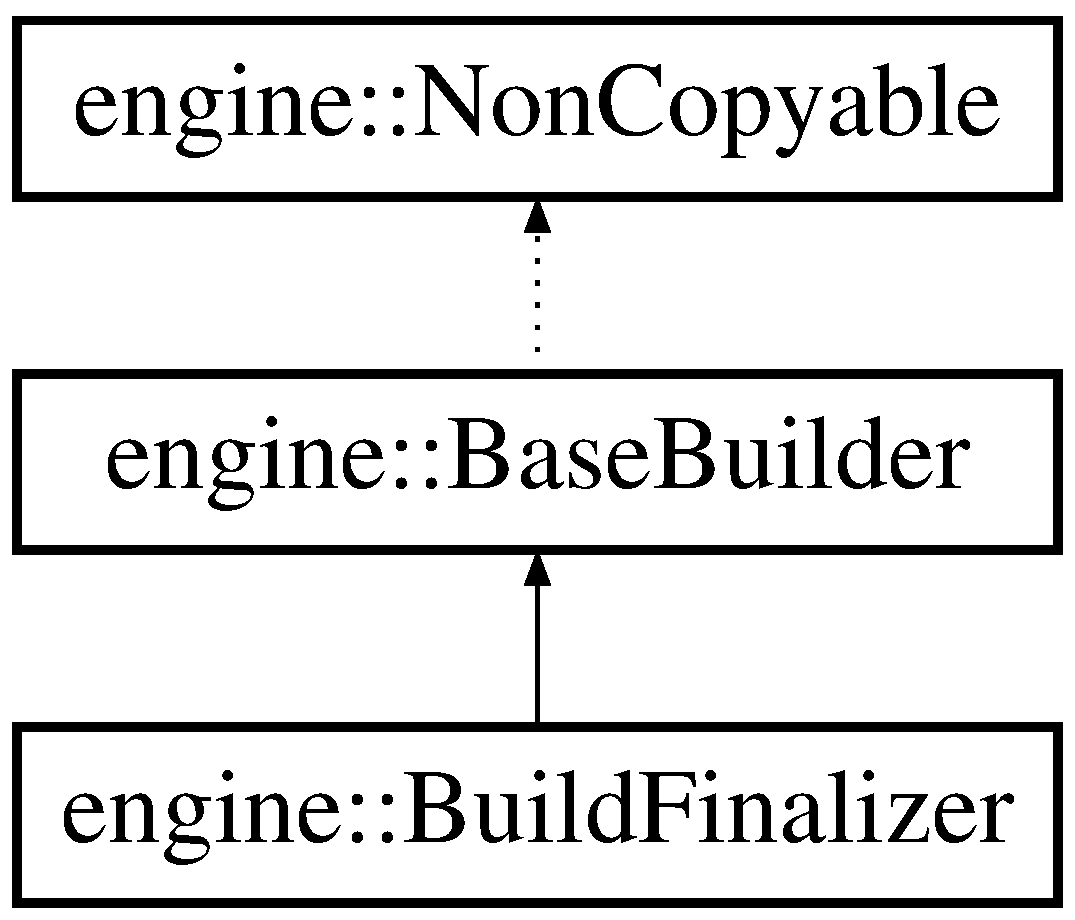
\includegraphics[height=3.000000cm]{a00011}
\end{center}
\end{figure}
\subsubsection*{Public Member Functions}
\begin{DoxyCompactItemize}
\item 
\hyperlink{a00011_abb814b037e8526d18118036c5142c96a}{Build\+Finalizer} ()=default
\item 
\hyperlink{a00011_ac23ed21d3f95a3c91ecdf900387fd9c6}{Build\+Finalizer} (\hyperlink{a00011}{Build\+Finalizer} \&\&)
\item 
void \hyperlink{a00011_a1a1fa8cbc1658b9a0240845c9335ab47}{build} ()
\end{DoxyCompactItemize}
\subsubsection*{Protected Member Functions}
\begin{DoxyCompactItemize}
\item 
void \hyperlink{a00005_a52fb449fadc5d3a074e3fc7bfb56744b}{add\+Module} (const Context\+Module\+Type value)
\item 
void \hyperlink{a00005_a20c5dafa6892142bc352c13a5f3ac09a}{set\+Application} (std\+::unique\+\_\+ptr$<$ \hyperlink{a00002}{Application} $>$ app)
\item 
void \hyperlink{a00005_a641fb06484bdb07220f445f14db8c0e7}{set\+Window\+Manager} (std\+::unique\+\_\+ptr$<$ \hyperlink{a00087}{Window\+Manager} $>$ manager)
\item 
void \hyperlink{a00005_a52b490a3ef4d2a5b5b7e8e0f82d9a27c}{set\+Event\+Manager} (std\+::unique\+\_\+ptr$<$ \hyperlink{a00034}{Event\+Manager} $>$ manager)
\item 
void \hyperlink{a00005_af23e3bdfb30ca9f2076cacc9029d96c2}{set\+Initialized} ()
\end{DoxyCompactItemize}


\subsubsection{Detailed Description}
Last build step. Ensure that the build process reaches the end of the creation. Without this build phase the context cannot be used. 

Definition at line 12 of file Build\+Finalizer.\+h.



\subsubsection{Constructor \& Destructor Documentation}
\index{engine\+::\+Build\+Finalizer@{engine\+::\+Build\+Finalizer}!Build\+Finalizer@{Build\+Finalizer}}
\index{Build\+Finalizer@{Build\+Finalizer}!engine\+::\+Build\+Finalizer@{engine\+::\+Build\+Finalizer}}
\paragraph[{\texorpdfstring{Build\+Finalizer()=default}{BuildFinalizer()=default}}]{\setlength{\rightskip}{0pt plus 5cm}engine\+::\+Build\+Finalizer\+::\+Build\+Finalizer (
\begin{DoxyParamCaption}
{}
\end{DoxyParamCaption}
)\hspace{0.3cm}{\ttfamily [default]}}\hypertarget{a00011_abb814b037e8526d18118036c5142c96a}{}\label{a00011_abb814b037e8526d18118036c5142c96a}
Defualt constructor \index{engine\+::\+Build\+Finalizer@{engine\+::\+Build\+Finalizer}!Build\+Finalizer@{Build\+Finalizer}}
\index{Build\+Finalizer@{Build\+Finalizer}!engine\+::\+Build\+Finalizer@{engine\+::\+Build\+Finalizer}}
\paragraph[{\texorpdfstring{Build\+Finalizer(\+Build\+Finalizer \&\&)}{BuildFinalizer(BuildFinalizer &&)}}]{\setlength{\rightskip}{0pt plus 5cm}engine\+::\+Build\+Finalizer\+::\+Build\+Finalizer (
\begin{DoxyParamCaption}
\item[{{\bf Build\+Finalizer} \&\&}]{}
\end{DoxyParamCaption}
)\hspace{0.3cm}{\ttfamily [inline]}}\hypertarget{a00011_ac23ed21d3f95a3c91ecdf900387fd9c6}{}\label{a00011_ac23ed21d3f95a3c91ecdf900387fd9c6}
Moveable 

Definition at line 18 of file Build\+Finalizer.\+h.



\subsubsection{Member Function Documentation}
\index{engine\+::\+Build\+Finalizer@{engine\+::\+Build\+Finalizer}!add\+Module@{add\+Module}}
\index{add\+Module@{add\+Module}!engine\+::\+Build\+Finalizer@{engine\+::\+Build\+Finalizer}}
\paragraph[{\texorpdfstring{add\+Module(const Context\+Module\+Type value)}{addModule(const ContextModuleType value)}}]{\setlength{\rightskip}{0pt plus 5cm}void engine\+::\+Base\+Builder\+::add\+Module (
\begin{DoxyParamCaption}
\item[{const Context\+Module\+Type}]{value}
\end{DoxyParamCaption}
)\hspace{0.3cm}{\ttfamily [protected]}, {\ttfamily [inherited]}}\hypertarget{a00005_a52fb449fadc5d3a074e3fc7bfb56744b}{}\label{a00005_a52fb449fadc5d3a074e3fc7bfb56744b}
Add a module type which is initialized during build phase 
\begin{DoxyParams}{Parameters}
{\em value} & Module which is initialized successfully \\
\hline
\end{DoxyParams}


Referenced by engine\+::\+Base\+Builder\+::$\sim$\+Base\+Builder().

\index{engine\+::\+Build\+Finalizer@{engine\+::\+Build\+Finalizer}!build@{build}}
\index{build@{build}!engine\+::\+Build\+Finalizer@{engine\+::\+Build\+Finalizer}}
\paragraph[{\texorpdfstring{build()}{build()}}]{\setlength{\rightskip}{0pt plus 5cm}void engine\+::\+Build\+Finalizer\+::build (
\begin{DoxyParamCaption}
{}
\end{DoxyParamCaption}
)}\hypertarget{a00011_a1a1fa8cbc1658b9a0240845c9335ab47}{}\label{a00011_a1a1fa8cbc1658b9a0240845c9335ab47}
Finish building process, no more step left. 

Referenced by Build\+Finalizer().

\index{engine\+::\+Build\+Finalizer@{engine\+::\+Build\+Finalizer}!set\+Application@{set\+Application}}
\index{set\+Application@{set\+Application}!engine\+::\+Build\+Finalizer@{engine\+::\+Build\+Finalizer}}
\paragraph[{\texorpdfstring{set\+Application(std\+::unique\+\_\+ptr$<$ Application $>$ app)}{setApplication(std::unique_ptr< Application > app)}}]{\setlength{\rightskip}{0pt plus 5cm}void engine\+::\+Base\+Builder\+::set\+Application (
\begin{DoxyParamCaption}
\item[{std\+::unique\+\_\+ptr$<$ {\bf Application} $>$}]{app}
\end{DoxyParamCaption}
)\hspace{0.3cm}{\ttfamily [protected]}, {\ttfamily [inherited]}}\hypertarget{a00005_a20c5dafa6892142bc352c13a5f3ac09a}{}\label{a00005_a20c5dafa6892142bc352c13a5f3ac09a}
Set the context application. 
\begin{DoxyParams}{Parameters}
{\em app} & \hyperlink{a00002}{Application} to use \\
\hline
\end{DoxyParams}


Referenced by engine\+::\+Base\+Builder\+::$\sim$\+Base\+Builder().

\index{engine\+::\+Build\+Finalizer@{engine\+::\+Build\+Finalizer}!set\+Event\+Manager@{set\+Event\+Manager}}
\index{set\+Event\+Manager@{set\+Event\+Manager}!engine\+::\+Build\+Finalizer@{engine\+::\+Build\+Finalizer}}
\paragraph[{\texorpdfstring{set\+Event\+Manager(std\+::unique\+\_\+ptr$<$ Event\+Manager $>$ manager)}{setEventManager(std::unique_ptr< EventManager > manager)}}]{\setlength{\rightskip}{0pt plus 5cm}void engine\+::\+Base\+Builder\+::set\+Event\+Manager (
\begin{DoxyParamCaption}
\item[{std\+::unique\+\_\+ptr$<$ {\bf Event\+Manager} $>$}]{manager}
\end{DoxyParamCaption}
)\hspace{0.3cm}{\ttfamily [protected]}, {\ttfamily [inherited]}}\hypertarget{a00005_a52b490a3ef4d2a5b5b7e8e0f82d9a27c}{}\label{a00005_a52b490a3ef4d2a5b5b7e8e0f82d9a27c}
Set the event manager of the context. 
\begin{DoxyParams}{Parameters}
{\em manager} & window manager to use \\
\hline
\end{DoxyParams}


Referenced by engine\+::\+Base\+Builder\+::$\sim$\+Base\+Builder().

\index{engine\+::\+Build\+Finalizer@{engine\+::\+Build\+Finalizer}!set\+Initialized@{set\+Initialized}}
\index{set\+Initialized@{set\+Initialized}!engine\+::\+Build\+Finalizer@{engine\+::\+Build\+Finalizer}}
\paragraph[{\texorpdfstring{set\+Initialized()}{setInitialized()}}]{\setlength{\rightskip}{0pt plus 5cm}void engine\+::\+Base\+Builder\+::set\+Initialized (
\begin{DoxyParamCaption}
{}
\end{DoxyParamCaption}
)\hspace{0.3cm}{\ttfamily [protected]}, {\ttfamily [inherited]}}\hypertarget{a00005_af23e3bdfb30ca9f2076cacc9029d96c2}{}\label{a00005_af23e3bdfb30ca9f2076cacc9029d96c2}
When the environment is built up this function finalize the context. 

Referenced by engine\+::\+Base\+Builder\+::$\sim$\+Base\+Builder().

\index{engine\+::\+Build\+Finalizer@{engine\+::\+Build\+Finalizer}!set\+Window\+Manager@{set\+Window\+Manager}}
\index{set\+Window\+Manager@{set\+Window\+Manager}!engine\+::\+Build\+Finalizer@{engine\+::\+Build\+Finalizer}}
\paragraph[{\texorpdfstring{set\+Window\+Manager(std\+::unique\+\_\+ptr$<$ Window\+Manager $>$ manager)}{setWindowManager(std::unique_ptr< WindowManager > manager)}}]{\setlength{\rightskip}{0pt plus 5cm}void engine\+::\+Base\+Builder\+::set\+Window\+Manager (
\begin{DoxyParamCaption}
\item[{std\+::unique\+\_\+ptr$<$ {\bf Window\+Manager} $>$}]{manager}
\end{DoxyParamCaption}
)\hspace{0.3cm}{\ttfamily [protected]}, {\ttfamily [inherited]}}\hypertarget{a00005_a641fb06484bdb07220f445f14db8c0e7}{}\label{a00005_a641fb06484bdb07220f445f14db8c0e7}
Set the window manager of the context. 
\begin{DoxyParams}{Parameters}
{\em manager} & window manager to use \\
\hline
\end{DoxyParams}


Referenced by engine\+::\+Base\+Builder\+::$\sim$\+Base\+Builder().



The documentation for this class was generated from the following file\+:\begin{DoxyCompactItemize}
\item 
E\+:/\+Programing/\+Projects/\+Engine\+Workspace/\+Common\+Libs/engine/include/engine/environment\+Builder/Build\+Finalizer.\+h\end{DoxyCompactItemize}

\hypertarget{a00012}{}\subsection{engine\+:\+:Context Class Reference}
\label{a00012}\index{engine\+::\+Context@{engine\+::\+Context}}


{\ttfamily \#include $<$E\+:/\+Programing/\+Projects/\+Engine\+Workspace/\+Common\+Libs/engine/include/engine/\+Context.\+h$>$}

Inheritance diagram for engine\+:\+:Context\+:\begin{figure}[H]
\begin{center}
\leavevmode
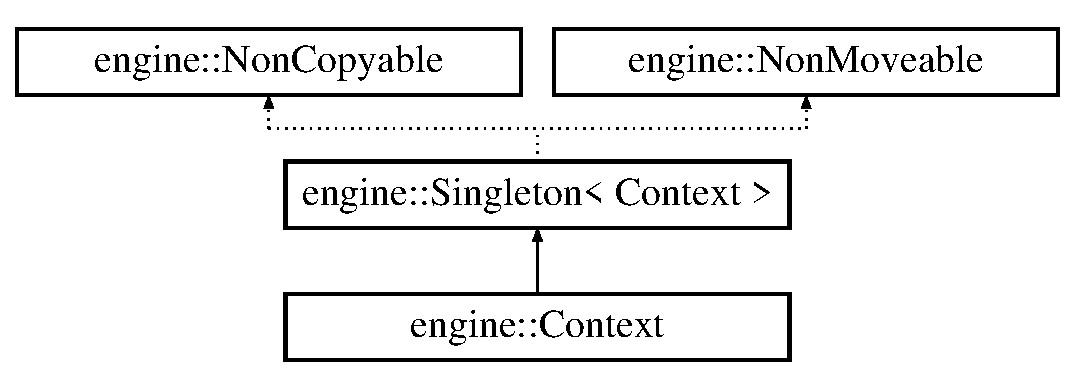
\includegraphics[height=3.000000cm]{a00012}
\end{center}
\end{figure}
\subsubsection*{Public Member Functions}
\begin{DoxyCompactItemize}
\item 
\hyperlink{a00002}{Application} $\ast$ \hyperlink{a00012_a6f657b971312b31eab5ff0b2148fab05}{get\+Application} ()
\end{DoxyCompactItemize}
\subsubsection*{Static Public Member Functions}
\begin{DoxyCompactItemize}
\item 
static \hyperlink{a00012}{Context} $\ast$ \hyperlink{a00069_a90ed1f21b1811a569eafccc78fcd12ca}{get\+Instance} ()
\item 
static void \hyperlink{a00069_a571e434c8ff771bf65de40f8a7b22076}{create\+Instance} (Args...\+args)
\item 
static void \hyperlink{a00069_a3fbed1f6a78cdf1d0c11467a3be61841}{release\+Instance} ()
\end{DoxyCompactItemize}
\subsubsection*{Protected Member Functions}
\begin{DoxyCompactItemize}
\item 
bool \hyperlink{a00012_ac532ff9bb55da7d1c351f1c2a0064f6d}{is\+Initialized} () const 
\end{DoxyCompactItemize}
\subsubsection*{Friends}
\begin{DoxyCompactItemize}
\item 
class {\bfseries Base\+Builder}\hypertarget{a00012_ad579f1883f887a1593ef8d2161435124}{}\label{a00012_ad579f1883f887a1593ef8d2161435124}

\end{DoxyCompactItemize}


\subsubsection{Detailed Description}
Engine\textquotesingle{}s context. This class contains the members which are necessary from everywhere in the application. 

Definition at line 14 of file Context.\+h.



\subsubsection{Member Function Documentation}
\index{engine\+::\+Context@{engine\+::\+Context}!create\+Instance@{create\+Instance}}
\index{create\+Instance@{create\+Instance}!engine\+::\+Context@{engine\+::\+Context}}
\paragraph[{\texorpdfstring{create\+Instance(\+Args...\+args)}{createInstance(Args...args)}}]{\setlength{\rightskip}{0pt plus 5cm}static void {\bf engine\+::\+Singleton}$<$ {\bf Context}  $>$\+::create\+Instance (
\begin{DoxyParamCaption}
\item[{Args...}]{args}
\end{DoxyParamCaption}
)\hspace{0.3cm}{\ttfamily [static]}, {\ttfamily [inherited]}}\hypertarget{a00069_a571e434c8ff771bf65de40f8a7b22076}{}\label{a00069_a571e434c8ff771bf65de40f8a7b22076}
Create an instance with the given arguments 
\begin{DoxyParams}{Parameters}
{\em creation} & arguments \\
\hline
\end{DoxyParams}
\index{engine\+::\+Context@{engine\+::\+Context}!get\+Application@{get\+Application}}
\index{get\+Application@{get\+Application}!engine\+::\+Context@{engine\+::\+Context}}
\paragraph[{\texorpdfstring{get\+Application()}{getApplication()}}]{\setlength{\rightskip}{0pt plus 5cm}{\bf Application}$\ast$ engine\+::\+Context\+::get\+Application (
\begin{DoxyParamCaption}
{}
\end{DoxyParamCaption}
)}\hypertarget{a00012_a6f657b971312b31eab5ff0b2148fab05}{}\label{a00012_a6f657b971312b31eab5ff0b2148fab05}
\begin{DoxyReturn}{Returns}
Returns the current appliation. 
\end{DoxyReturn}
\begin{DoxySeeAlso}{See also}
\hyperlink{a00002}{Application} 
\end{DoxySeeAlso}
\index{engine\+::\+Context@{engine\+::\+Context}!get\+Instance@{get\+Instance}}
\index{get\+Instance@{get\+Instance}!engine\+::\+Context@{engine\+::\+Context}}
\paragraph[{\texorpdfstring{get\+Instance()}{getInstance()}}]{\setlength{\rightskip}{0pt plus 5cm}static {\bf Context} $\ast$ {\bf engine\+::\+Singleton}$<$ {\bf Context}  $>$\+::get\+Instance (
\begin{DoxyParamCaption}
{}
\end{DoxyParamCaption}
)\hspace{0.3cm}{\ttfamily [static]}, {\ttfamily [inherited]}}\hypertarget{a00069_a90ed1f21b1811a569eafccc78fcd12ca}{}\label{a00069_a90ed1f21b1811a569eafccc78fcd12ca}
\begin{DoxyReturn}{Returns}
the instance object 
\end{DoxyReturn}
\index{engine\+::\+Context@{engine\+::\+Context}!is\+Initialized@{is\+Initialized}}
\index{is\+Initialized@{is\+Initialized}!engine\+::\+Context@{engine\+::\+Context}}
\paragraph[{\texorpdfstring{is\+Initialized() const }{isInitialized() const }}]{\setlength{\rightskip}{0pt plus 5cm}bool engine\+::\+Context\+::is\+Initialized (
\begin{DoxyParamCaption}
{}
\end{DoxyParamCaption}
) const\hspace{0.3cm}{\ttfamily [protected]}}\hypertarget{a00012_ac532ff9bb55da7d1c351f1c2a0064f6d}{}\label{a00012_ac532ff9bb55da7d1c351f1c2a0064f6d}
The context can be used only if it is initialized. Because the context creation is a complicated task, it is done in separate steps by builders. \index{engine\+::\+Context@{engine\+::\+Context}!release\+Instance@{release\+Instance}}
\index{release\+Instance@{release\+Instance}!engine\+::\+Context@{engine\+::\+Context}}
\paragraph[{\texorpdfstring{release\+Instance()}{releaseInstance()}}]{\setlength{\rightskip}{0pt plus 5cm}static void {\bf engine\+::\+Singleton}$<$ {\bf Context}  $>$\+::release\+Instance (
\begin{DoxyParamCaption}
{}
\end{DoxyParamCaption}
)\hspace{0.3cm}{\ttfamily [static]}, {\ttfamily [inherited]}}\hypertarget{a00069_a3fbed1f6a78cdf1d0c11467a3be61841}{}\label{a00069_a3fbed1f6a78cdf1d0c11467a3be61841}
Delete the instance 

The documentation for this class was generated from the following file\+:\begin{DoxyCompactItemize}
\item 
E\+:/\+Programing/\+Projects/\+Engine\+Workspace/\+Common\+Libs/engine/include/engine/Context.\+h\end{DoxyCompactItemize}

\hypertarget{a00013}{}\subsection{engine\+:\+:Context\+Builder Class Reference}
\label{a00013}\index{engine\+::\+Context\+Builder@{engine\+::\+Context\+Builder}}


{\ttfamily \#include $<$E\+:/\+Programing/\+Projects/\+Engine\+Workspace/\+Common\+Libs/engine/include/engine/environment\+Builder/\+Context\+Builder.\+h$>$}

Inheritance diagram for engine\+:\+:Context\+Builder\+:\begin{figure}[H]
\begin{center}
\leavevmode
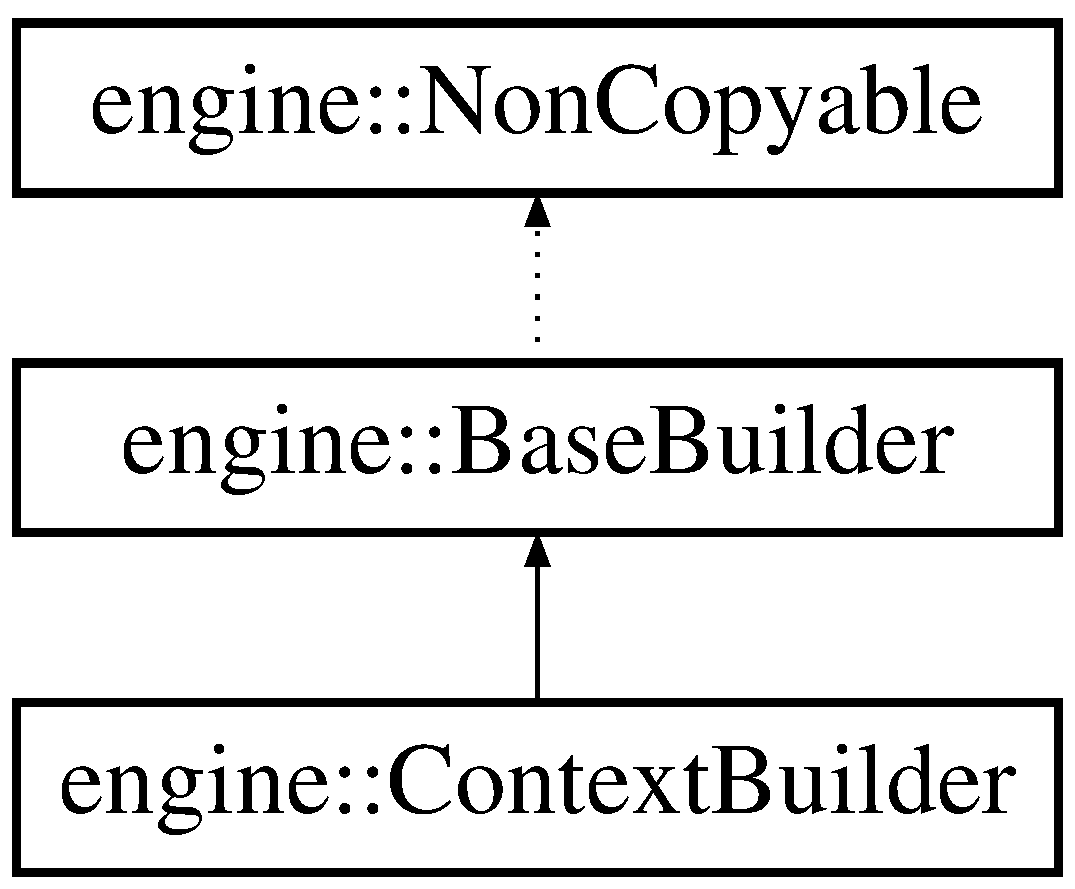
\includegraphics[height=3.000000cm]{a00013}
\end{center}
\end{figure}
\subsubsection*{Public Member Functions}
\begin{DoxyCompactItemize}
\item 
\hyperlink{a00013_aca8c1a2731d9f2da0d0cb3fa150c314c}{Context\+Builder} (const std\+::vector$<$ Context\+Module\+Type $>$ \&moduls)
\item 
\hyperlink{a00013_ae8a046bccdc9e1461de3f952e15df0e4}{Context\+Builder} (\hyperlink{a00013}{Context\+Builder} \&\&o)
\item 
\hyperlink{a00013_acbc8b557d2a1755b41dc4e39cfefaa79}{$\sim$\+Context\+Builder} ()
\item 
\hyperlink{a00003}{Application\+Builder} \hyperlink{a00013_a397a774fc36c66dda2ee90a56f4094e1}{build\+For\+Application} ()
\end{DoxyCompactItemize}
\subsubsection*{Protected Member Functions}
\begin{DoxyCompactItemize}
\item 
void \hyperlink{a00005_a52fb449fadc5d3a074e3fc7bfb56744b}{add\+Module} (const Context\+Module\+Type value)
\item 
void \hyperlink{a00005_a20c5dafa6892142bc352c13a5f3ac09a}{set\+Application} (std\+::unique\+\_\+ptr$<$ \hyperlink{a00002}{Application} $>$ app)
\item 
void \hyperlink{a00005_a641fb06484bdb07220f445f14db8c0e7}{set\+Window\+Manager} (std\+::unique\+\_\+ptr$<$ \hyperlink{a00087}{Window\+Manager} $>$ manager)
\item 
void \hyperlink{a00005_a52b490a3ef4d2a5b5b7e8e0f82d9a27c}{set\+Event\+Manager} (std\+::unique\+\_\+ptr$<$ \hyperlink{a00034}{Event\+Manager} $>$ manager)
\item 
void \hyperlink{a00005_af23e3bdfb30ca9f2076cacc9029d96c2}{set\+Initialized} ()
\end{DoxyCompactItemize}


\subsubsection{Detailed Description}
Creates the context which is the cornerstone of the environment 

Definition at line 16 of file Context\+Builder.\+h.



\subsubsection{Constructor \& Destructor Documentation}
\index{engine\+::\+Context\+Builder@{engine\+::\+Context\+Builder}!Context\+Builder@{Context\+Builder}}
\index{Context\+Builder@{Context\+Builder}!engine\+::\+Context\+Builder@{engine\+::\+Context\+Builder}}
\paragraph[{\texorpdfstring{Context\+Builder(const std\+::vector$<$ Context\+Module\+Type $>$ \&moduls)}{ContextBuilder(const std::vector< ContextModuleType > &moduls)}}]{\setlength{\rightskip}{0pt plus 5cm}engine\+::\+Context\+Builder\+::\+Context\+Builder (
\begin{DoxyParamCaption}
\item[{const std\+::vector$<$ Context\+Module\+Type $>$ \&}]{moduls}
\end{DoxyParamCaption}
)}\hypertarget{a00013_aca8c1a2731d9f2da0d0cb3fa150c314c}{}\label{a00013_aca8c1a2731d9f2da0d0cb3fa150c314c}
Create the context. This build phase will also initialize the different kind of modules. 
\begin{DoxyParams}{Parameters}
{\em moduls} & Modules which will be initialized during the build. \\
\hline
\end{DoxyParams}
\index{engine\+::\+Context\+Builder@{engine\+::\+Context\+Builder}!Context\+Builder@{Context\+Builder}}
\index{Context\+Builder@{Context\+Builder}!engine\+::\+Context\+Builder@{engine\+::\+Context\+Builder}}
\paragraph[{\texorpdfstring{Context\+Builder(\+Context\+Builder \&\&o)}{ContextBuilder(ContextBuilder &&o)}}]{\setlength{\rightskip}{0pt plus 5cm}engine\+::\+Context\+Builder\+::\+Context\+Builder (
\begin{DoxyParamCaption}
\item[{{\bf Context\+Builder} \&\&}]{o}
\end{DoxyParamCaption}
)}\hypertarget{a00013_ae8a046bccdc9e1461de3f952e15df0e4}{}\label{a00013_ae8a046bccdc9e1461de3f952e15df0e4}
Moveable \index{engine\+::\+Context\+Builder@{engine\+::\+Context\+Builder}!````~Context\+Builder@{$\sim$\+Context\+Builder}}
\index{````~Context\+Builder@{$\sim$\+Context\+Builder}!engine\+::\+Context\+Builder@{engine\+::\+Context\+Builder}}
\paragraph[{\texorpdfstring{$\sim$\+Context\+Builder()}{~ContextBuilder()}}]{\setlength{\rightskip}{0pt plus 5cm}engine\+::\+Context\+Builder\+::$\sim$\+Context\+Builder (
\begin{DoxyParamCaption}
{}
\end{DoxyParamCaption}
)}\hypertarget{a00013_acbc8b557d2a1755b41dc4e39cfefaa79}{}\label{a00013_acbc8b557d2a1755b41dc4e39cfefaa79}
Destructor for P\+I\+M\+PL 

\subsubsection{Member Function Documentation}
\index{engine\+::\+Context\+Builder@{engine\+::\+Context\+Builder}!add\+Module@{add\+Module}}
\index{add\+Module@{add\+Module}!engine\+::\+Context\+Builder@{engine\+::\+Context\+Builder}}
\paragraph[{\texorpdfstring{add\+Module(const Context\+Module\+Type value)}{addModule(const ContextModuleType value)}}]{\setlength{\rightskip}{0pt plus 5cm}void engine\+::\+Base\+Builder\+::add\+Module (
\begin{DoxyParamCaption}
\item[{const Context\+Module\+Type}]{value}
\end{DoxyParamCaption}
)\hspace{0.3cm}{\ttfamily [protected]}, {\ttfamily [inherited]}}\hypertarget{a00005_a52fb449fadc5d3a074e3fc7bfb56744b}{}\label{a00005_a52fb449fadc5d3a074e3fc7bfb56744b}
Add a module type which is initialized during build phase 
\begin{DoxyParams}{Parameters}
{\em value} & Module which is initialized successfully \\
\hline
\end{DoxyParams}


Referenced by engine\+::\+Base\+Builder\+::$\sim$\+Base\+Builder().

\index{engine\+::\+Context\+Builder@{engine\+::\+Context\+Builder}!build\+For\+Application@{build\+For\+Application}}
\index{build\+For\+Application@{build\+For\+Application}!engine\+::\+Context\+Builder@{engine\+::\+Context\+Builder}}
\paragraph[{\texorpdfstring{build\+For\+Application()}{buildForApplication()}}]{\setlength{\rightskip}{0pt plus 5cm}{\bf Application\+Builder} engine\+::\+Context\+Builder\+::build\+For\+Application (
\begin{DoxyParamCaption}
{}
\end{DoxyParamCaption}
)}\hypertarget{a00013_a397a774fc36c66dda2ee90a56f4094e1}{}\label{a00013_a397a774fc36c66dda2ee90a56f4094e1}
Build the context and init the next step. \begin{DoxyReturn}{Returns}
Returns the next building phase. 
\end{DoxyReturn}
\index{engine\+::\+Context\+Builder@{engine\+::\+Context\+Builder}!set\+Application@{set\+Application}}
\index{set\+Application@{set\+Application}!engine\+::\+Context\+Builder@{engine\+::\+Context\+Builder}}
\paragraph[{\texorpdfstring{set\+Application(std\+::unique\+\_\+ptr$<$ Application $>$ app)}{setApplication(std::unique_ptr< Application > app)}}]{\setlength{\rightskip}{0pt plus 5cm}void engine\+::\+Base\+Builder\+::set\+Application (
\begin{DoxyParamCaption}
\item[{std\+::unique\+\_\+ptr$<$ {\bf Application} $>$}]{app}
\end{DoxyParamCaption}
)\hspace{0.3cm}{\ttfamily [protected]}, {\ttfamily [inherited]}}\hypertarget{a00005_a20c5dafa6892142bc352c13a5f3ac09a}{}\label{a00005_a20c5dafa6892142bc352c13a5f3ac09a}
Set the context application. 
\begin{DoxyParams}{Parameters}
{\em app} & \hyperlink{a00002}{Application} to use \\
\hline
\end{DoxyParams}


Referenced by engine\+::\+Base\+Builder\+::$\sim$\+Base\+Builder().

\index{engine\+::\+Context\+Builder@{engine\+::\+Context\+Builder}!set\+Event\+Manager@{set\+Event\+Manager}}
\index{set\+Event\+Manager@{set\+Event\+Manager}!engine\+::\+Context\+Builder@{engine\+::\+Context\+Builder}}
\paragraph[{\texorpdfstring{set\+Event\+Manager(std\+::unique\+\_\+ptr$<$ Event\+Manager $>$ manager)}{setEventManager(std::unique_ptr< EventManager > manager)}}]{\setlength{\rightskip}{0pt plus 5cm}void engine\+::\+Base\+Builder\+::set\+Event\+Manager (
\begin{DoxyParamCaption}
\item[{std\+::unique\+\_\+ptr$<$ {\bf Event\+Manager} $>$}]{manager}
\end{DoxyParamCaption}
)\hspace{0.3cm}{\ttfamily [protected]}, {\ttfamily [inherited]}}\hypertarget{a00005_a52b490a3ef4d2a5b5b7e8e0f82d9a27c}{}\label{a00005_a52b490a3ef4d2a5b5b7e8e0f82d9a27c}
Set the event manager of the context. 
\begin{DoxyParams}{Parameters}
{\em manager} & window manager to use \\
\hline
\end{DoxyParams}


Referenced by engine\+::\+Base\+Builder\+::$\sim$\+Base\+Builder().

\index{engine\+::\+Context\+Builder@{engine\+::\+Context\+Builder}!set\+Initialized@{set\+Initialized}}
\index{set\+Initialized@{set\+Initialized}!engine\+::\+Context\+Builder@{engine\+::\+Context\+Builder}}
\paragraph[{\texorpdfstring{set\+Initialized()}{setInitialized()}}]{\setlength{\rightskip}{0pt plus 5cm}void engine\+::\+Base\+Builder\+::set\+Initialized (
\begin{DoxyParamCaption}
{}
\end{DoxyParamCaption}
)\hspace{0.3cm}{\ttfamily [protected]}, {\ttfamily [inherited]}}\hypertarget{a00005_af23e3bdfb30ca9f2076cacc9029d96c2}{}\label{a00005_af23e3bdfb30ca9f2076cacc9029d96c2}
When the environment is built up this function finalize the context. 

Referenced by engine\+::\+Base\+Builder\+::$\sim$\+Base\+Builder().

\index{engine\+::\+Context\+Builder@{engine\+::\+Context\+Builder}!set\+Window\+Manager@{set\+Window\+Manager}}
\index{set\+Window\+Manager@{set\+Window\+Manager}!engine\+::\+Context\+Builder@{engine\+::\+Context\+Builder}}
\paragraph[{\texorpdfstring{set\+Window\+Manager(std\+::unique\+\_\+ptr$<$ Window\+Manager $>$ manager)}{setWindowManager(std::unique_ptr< WindowManager > manager)}}]{\setlength{\rightskip}{0pt plus 5cm}void engine\+::\+Base\+Builder\+::set\+Window\+Manager (
\begin{DoxyParamCaption}
\item[{std\+::unique\+\_\+ptr$<$ {\bf Window\+Manager} $>$}]{manager}
\end{DoxyParamCaption}
)\hspace{0.3cm}{\ttfamily [protected]}, {\ttfamily [inherited]}}\hypertarget{a00005_a641fb06484bdb07220f445f14db8c0e7}{}\label{a00005_a641fb06484bdb07220f445f14db8c0e7}
Set the window manager of the context. 
\begin{DoxyParams}{Parameters}
{\em manager} & window manager to use \\
\hline
\end{DoxyParams}


Referenced by engine\+::\+Base\+Builder\+::$\sim$\+Base\+Builder().



The documentation for this class was generated from the following file\+:\begin{DoxyCompactItemize}
\item 
E\+:/\+Programing/\+Projects/\+Engine\+Workspace/\+Common\+Libs/engine/include/engine/environment\+Builder/Context\+Builder.\+h\end{DoxyCompactItemize}

\hypertarget{a00014}{}\subsection{engine\+:\+:Context\+Module\+\_\+traits$<$ type $>$ Struct Template Reference}
\label{a00014}\index{engine\+::\+Context\+Module\+\_\+traits$<$ type $>$@{engine\+::\+Context\+Module\+\_\+traits$<$ type $>$}}


{\ttfamily \#include $<$E\+:/\+Programing/\+Projects/\+Engine\+Workspace/\+Common\+Libs/engine/include/engine/\+Module\+Definitions.\+h$>$}



\subsubsection{Detailed Description}
\subsubsection*{template$<$Context\+Module\+Type type$>$\\*
struct engine\+::\+Context\+Module\+\_\+traits$<$ type $>$}

Meta data for module types. 

Definition at line 30 of file Module\+Definitions.\+h.



The documentation for this struct was generated from the following file\+:\begin{DoxyCompactItemize}
\item 
E\+:/\+Programing/\+Projects/\+Engine\+Workspace/\+Common\+Libs/engine/include/engine/Module\+Definitions.\+h\end{DoxyCompactItemize}

\hypertarget{a00015}{}\subsection{engine\+:\+:Context\+Module\+\_\+traits$<$ Context\+Module\+Type\+:\+:Glfw $>$ Struct Template Reference}
\label{a00015}\index{engine\+::\+Context\+Module\+\_\+traits$<$ Context\+Module\+Type\+::\+Glfw $>$@{engine\+::\+Context\+Module\+\_\+traits$<$ Context\+Module\+Type\+::\+Glfw $>$}}
\subsubsection*{Static Public Attributes}
\begin{DoxyCompactItemize}
\item 
static const Context\+Module\+Classification {\bfseries classification}\hypertarget{a00015_a39b0ff37cddf6a8c8e7b2ff7524fc4b1}{}\label{a00015_a39b0ff37cddf6a8c8e7b2ff7524fc4b1}

\item 
static const std\+::string {\bfseries name}\hypertarget{a00015_ab441070b94df5afc85da1c6eeff0963a}{}\label{a00015_ab441070b94df5afc85da1c6eeff0963a}

\end{DoxyCompactItemize}


\subsubsection{Detailed Description}
\subsubsection*{template$<$$>$\\*
struct engine\+::\+Context\+Module\+\_\+traits$<$ Context\+Module\+Type\+::\+Glfw $>$}



Definition at line 35 of file Module\+Definitions.\+h.



The documentation for this struct was generated from the following file\+:\begin{DoxyCompactItemize}
\item 
E\+:/\+Programing/\+Projects/\+Engine\+Workspace/\+Common\+Libs/engine/include/engine/Module\+Definitions.\+h\end{DoxyCompactItemize}

\hypertarget{a00016}{}\subsection{engine\+:\+:Context\+Module\+\_\+traits$<$ Context\+Module\+Type\+:\+:Sdl $>$ Struct Template Reference}
\label{a00016}\index{engine\+::\+Context\+Module\+\_\+traits$<$ Context\+Module\+Type\+::\+Sdl $>$@{engine\+::\+Context\+Module\+\_\+traits$<$ Context\+Module\+Type\+::\+Sdl $>$}}
\subsubsection*{Static Public Attributes}
\begin{DoxyCompactItemize}
\item 
static const Context\+Module\+Classification {\bfseries classification}\hypertarget{a00016_a29e011a5450db531464fa89705f7fd16}{}\label{a00016_a29e011a5450db531464fa89705f7fd16}

\item 
static const std\+::string {\bfseries name}\hypertarget{a00016_aaffd24695252e25d995dcd03dde5f0ba}{}\label{a00016_aaffd24695252e25d995dcd03dde5f0ba}

\end{DoxyCompactItemize}


\subsubsection{Detailed Description}
\subsubsection*{template$<$$>$\\*
struct engine\+::\+Context\+Module\+\_\+traits$<$ Context\+Module\+Type\+::\+Sdl $>$}



Definition at line 44 of file Module\+Definitions.\+h.



The documentation for this struct was generated from the following file\+:\begin{DoxyCompactItemize}
\item 
E\+:/\+Programing/\+Projects/\+Engine\+Workspace/\+Common\+Libs/engine/include/engine/Module\+Definitions.\+h\end{DoxyCompactItemize}

\hypertarget{a00017}{}\subsection{engine\+:\+:Context\+Module\+\_\+traits$<$ Context\+Module\+Type\+:\+:Win\+Api $>$ Struct Template Reference}
\label{a00017}\index{engine\+::\+Context\+Module\+\_\+traits$<$ Context\+Module\+Type\+::\+Win\+Api $>$@{engine\+::\+Context\+Module\+\_\+traits$<$ Context\+Module\+Type\+::\+Win\+Api $>$}}
\subsubsection*{Static Public Attributes}
\begin{DoxyCompactItemize}
\item 
static const Context\+Module\+Classification {\bfseries classification}\hypertarget{a00017_a655b512a8ed83e8d2b78642e9654cc99}{}\label{a00017_a655b512a8ed83e8d2b78642e9654cc99}

\item 
static const std\+::string {\bfseries name}\hypertarget{a00017_a1f9f8f5e908291aed01a5e0845208d23}{}\label{a00017_a1f9f8f5e908291aed01a5e0845208d23}

\end{DoxyCompactItemize}


\subsubsection{Detailed Description}
\subsubsection*{template$<$$>$\\*
struct engine\+::\+Context\+Module\+\_\+traits$<$ Context\+Module\+Type\+::\+Win\+Api $>$}



Definition at line 52 of file Module\+Definitions.\+h.



The documentation for this struct was generated from the following file\+:\begin{DoxyCompactItemize}
\item 
E\+:/\+Programing/\+Projects/\+Engine\+Workspace/\+Common\+Libs/engine/include/engine/Module\+Definitions.\+h\end{DoxyCompactItemize}

\hypertarget{a00018}{}\subsection{engine\+:\+:glfw\+:\+:Core Class Reference}
\label{a00018}\index{engine\+::glfw\+::\+Core@{engine\+::glfw\+::\+Core}}


{\ttfamily \#include $<$E\+:/\+Programing/\+Projects/\+Engine\+Workspace/\+Common\+Libs/engine/include/engine/modules/glfw/\+Core.\+h$>$}

\subsubsection*{Static Public Member Functions}
\begin{DoxyCompactItemize}
\item 
static bool \hyperlink{a00018_a54bfba36517cae500798aae57ce31c12}{init} ()
\end{DoxyCompactItemize}


\subsubsection{Detailed Description}
Glfw module core module. 

Definition at line 10 of file Core.\+h.



\subsubsection{Member Function Documentation}
\index{engine\+::glfw\+::\+Core@{engine\+::glfw\+::\+Core}!init@{init}}
\index{init@{init}!engine\+::glfw\+::\+Core@{engine\+::glfw\+::\+Core}}
\paragraph[{\texorpdfstring{init()}{init()}}]{\setlength{\rightskip}{0pt plus 5cm}static bool engine\+::glfw\+::\+Core\+::init (
\begin{DoxyParamCaption}
{}
\end{DoxyParamCaption}
)\hspace{0.3cm}{\ttfamily [static]}}\hypertarget{a00018_a54bfba36517cae500798aae57ce31c12}{}\label{a00018_a54bfba36517cae500798aae57ce31c12}
Initialize the module. \begin{DoxyReturn}{Returns}
True if the init was successfull. 
\end{DoxyReturn}


The documentation for this class was generated from the following file\+:\begin{DoxyCompactItemize}
\item 
E\+:/\+Programing/\+Projects/\+Engine\+Workspace/\+Common\+Libs/engine/include/engine/modules/glfw/Core.\+h\end{DoxyCompactItemize}

\hypertarget{a00019}{}\subsection{engine\+:\+:sdl\+:\+:Core Class Reference}
\label{a00019}\index{engine\+::sdl\+::\+Core@{engine\+::sdl\+::\+Core}}


{\ttfamily \#include $<$E\+:/\+Programing/\+Projects/\+Engine\+Workspace/\+Common\+Libs/engine/include/engine/modules/sdl/\+Core.\+h$>$}

\subsubsection*{Static Public Member Functions}
\begin{DoxyCompactItemize}
\item 
static bool \hyperlink{a00019_a19e45cac77785c72dfb09888d65d4bcc}{init} ()
\end{DoxyCompactItemize}


\subsubsection{Detailed Description}
Sdl module core module. 

Definition at line 10 of file Core.\+h.



\subsubsection{Member Function Documentation}
\index{engine\+::sdl\+::\+Core@{engine\+::sdl\+::\+Core}!init@{init}}
\index{init@{init}!engine\+::sdl\+::\+Core@{engine\+::sdl\+::\+Core}}
\paragraph[{\texorpdfstring{init()}{init()}}]{\setlength{\rightskip}{0pt plus 5cm}static bool engine\+::sdl\+::\+Core\+::init (
\begin{DoxyParamCaption}
{}
\end{DoxyParamCaption}
)\hspace{0.3cm}{\ttfamily [static]}}\hypertarget{a00019_a19e45cac77785c72dfb09888d65d4bcc}{}\label{a00019_a19e45cac77785c72dfb09888d65d4bcc}
Initialize the module. \begin{DoxyReturn}{Returns}
True if the init was successfull. 
\end{DoxyReturn}


The documentation for this class was generated from the following file\+:\begin{DoxyCompactItemize}
\item 
E\+:/\+Programing/\+Projects/\+Engine\+Workspace/\+Common\+Libs/engine/include/engine/modules/sdl/Core.\+h\end{DoxyCompactItemize}

\hypertarget{a00020}{}\subsection{engine\+:\+:winapi\+:\+:Core Class Reference}
\label{a00020}\index{engine\+::winapi\+::\+Core@{engine\+::winapi\+::\+Core}}


{\ttfamily \#include $<$E\+:/\+Programing/\+Projects/\+Engine\+Workspace/\+Common\+Libs/engine/include/engine/modules/winapi/\+Core.\+h$>$}

\subsubsection*{Static Public Member Functions}
\begin{DoxyCompactItemize}
\item 
static bool \hyperlink{a00020_a908c19ff86e54cf37ddcddeb55e610ae}{init} ()
\end{DoxyCompactItemize}


\subsubsection{Detailed Description}
Win\+Api \hyperlink{a00020}{Core} module. 

Definition at line 8 of file Core.\+h.



\subsubsection{Member Function Documentation}
\index{engine\+::winapi\+::\+Core@{engine\+::winapi\+::\+Core}!init@{init}}
\index{init@{init}!engine\+::winapi\+::\+Core@{engine\+::winapi\+::\+Core}}
\paragraph[{\texorpdfstring{init()}{init()}}]{\setlength{\rightskip}{0pt plus 5cm}static bool engine\+::winapi\+::\+Core\+::init (
\begin{DoxyParamCaption}
{}
\end{DoxyParamCaption}
)\hspace{0.3cm}{\ttfamily [static]}}\hypertarget{a00020_a908c19ff86e54cf37ddcddeb55e610ae}{}\label{a00020_a908c19ff86e54cf37ddcddeb55e610ae}
Initialize the module. \begin{DoxyReturn}{Returns}
Returns true when the initialization was successful. 
\end{DoxyReturn}


The documentation for this class was generated from the following file\+:\begin{DoxyCompactItemize}
\item 
E\+:/\+Programing/\+Projects/\+Engine\+Workspace/\+Common\+Libs/engine/include/engine/modules/winapi/Core.\+h\end{DoxyCompactItemize}

\hypertarget{a00021}{}\subsection{engine\+:\+:Counted\+Object$<$ T $>$ Struct Template Reference}
\label{a00021}\index{engine\+::\+Counted\+Object$<$ T $>$@{engine\+::\+Counted\+Object$<$ T $>$}}


{\ttfamily \#include $<$E\+:/\+Programing/\+Projects/\+Engine\+Workspace/\+Common\+Libs/engine/include/engine/utils/\+Counted\+Object.\+h$>$}

\subsubsection*{Static Public Member Functions}
\begin{DoxyCompactItemize}
\item 
static uint64\+\_\+t \hyperlink{a00021_a693c549c84cd89d45e46018f9d2f1420}{get\+Object\+Count} () const 
\end{DoxyCompactItemize}
\subsubsection*{Protected Member Functions}
\begin{DoxyCompactItemize}
\item 
\hyperlink{a00021_a9f4f5b1610e616b8c7ffa347c99729e3}{Counted\+Object} ()
\item 
virtual \hyperlink{a00021_a8858bb0d52059b19ffa684c7dc716fe3}{$\sim$\+Counted\+Object} ()
\end{DoxyCompactItemize}


\subsubsection{Detailed Description}
\subsubsection*{template$<$typename T$>$\\*
struct engine\+::\+Counted\+Object$<$ T $>$}

Base class to check object creation. Thread safe. 
\begin{DoxyTemplParams}{Template Parameters}
{\em T} & The class which creation will counted. \\
\hline
\end{DoxyTemplParams}


Definition at line 14 of file Counted\+Object.\+h.



\subsubsection{Constructor \& Destructor Documentation}
\index{engine\+::\+Counted\+Object@{engine\+::\+Counted\+Object}!Counted\+Object@{Counted\+Object}}
\index{Counted\+Object@{Counted\+Object}!engine\+::\+Counted\+Object@{engine\+::\+Counted\+Object}}
\paragraph[{\texorpdfstring{Counted\+Object()}{CountedObject()}}]{\setlength{\rightskip}{0pt plus 5cm}template$<$typename T $>$ {\bf engine\+::\+Counted\+Object}$<$ T $>$\+::{\bf Counted\+Object} (
\begin{DoxyParamCaption}
{}
\end{DoxyParamCaption}
)\hspace{0.3cm}{\ttfamily [inline]}, {\ttfamily [protected]}}\hypertarget{a00021_a9f4f5b1610e616b8c7ffa347c99729e3}{}\label{a00021_a9f4f5b1610e616b8c7ffa347c99729e3}
Constructor for counting 

Definition at line 32 of file Counted\+Object.\+h.

\index{engine\+::\+Counted\+Object@{engine\+::\+Counted\+Object}!````~Counted\+Object@{$\sim$\+Counted\+Object}}
\index{````~Counted\+Object@{$\sim$\+Counted\+Object}!engine\+::\+Counted\+Object@{engine\+::\+Counted\+Object}}
\paragraph[{\texorpdfstring{$\sim$\+Counted\+Object()}{~CountedObject()}}]{\setlength{\rightskip}{0pt plus 5cm}template$<$typename T $>$ virtual {\bf engine\+::\+Counted\+Object}$<$ T $>$\+::$\sim${\bf Counted\+Object} (
\begin{DoxyParamCaption}
{}
\end{DoxyParamCaption}
)\hspace{0.3cm}{\ttfamily [inline]}, {\ttfamily [protected]}, {\ttfamily [virtual]}}\hypertarget{a00021_a8858bb0d52059b19ffa684c7dc716fe3}{}\label{a00021_a8858bb0d52059b19ffa684c7dc716fe3}
Destructor for counting 

Definition at line 40 of file Counted\+Object.\+h.



\subsubsection{Member Function Documentation}
\index{engine\+::\+Counted\+Object@{engine\+::\+Counted\+Object}!get\+Object\+Count@{get\+Object\+Count}}
\index{get\+Object\+Count@{get\+Object\+Count}!engine\+::\+Counted\+Object@{engine\+::\+Counted\+Object}}
\paragraph[{\texorpdfstring{get\+Object\+Count() const }{getObjectCount() const }}]{\setlength{\rightskip}{0pt plus 5cm}template$<$typename T $>$ static uint64\+\_\+t {\bf engine\+::\+Counted\+Object}$<$ T $>$\+::get\+Object\+Count (
\begin{DoxyParamCaption}
{}
\end{DoxyParamCaption}
) const\hspace{0.3cm}{\ttfamily [inline]}, {\ttfamily [static]}}\hypertarget{a00021_a693c549c84cd89d45e46018f9d2f1420}{}\label{a00021_a693c549c84cd89d45e46018f9d2f1420}
\begin{DoxyReturn}{Returns}
Retuns how much object is still alive from the given class. 
\end{DoxyReturn}


Definition at line 20 of file Counted\+Object.\+h.



The documentation for this struct was generated from the following file\+:\begin{DoxyCompactItemize}
\item 
E\+:/\+Programing/\+Projects/\+Engine\+Workspace/\+Common\+Libs/engine/include/engine/utils/Counted\+Object.\+h\end{DoxyCompactItemize}

\hypertarget{a00022}{}\subsection{engine\+:\+:Custom\+Placeholder$<$ int $>$ Struct Template Reference}
\label{a00022}\index{engine\+::\+Custom\+Placeholder$<$ int $>$@{engine\+::\+Custom\+Placeholder$<$ int $>$}}


{\ttfamily \#include $<$E\+:/\+Programing/\+Projects/\+Engine\+Workspace/\+Common\+Libs/engine/include/engine/utils/\+Custom\+Placeholder.\+h$>$}



\subsubsection{Detailed Description}
\subsubsection*{template$<$int$>$\\*
struct engine\+::\+Custom\+Placeholder$<$ int $>$}

Custom amount of placeholder for funciton binding 

Definition at line 8 of file Custom\+Placeholder.\+h.



The documentation for this struct was generated from the following file\+:\begin{DoxyCompactItemize}
\item 
E\+:/\+Programing/\+Projects/\+Engine\+Workspace/\+Common\+Libs/engine/include/engine/utils/Custom\+Placeholder.\+h\end{DoxyCompactItemize}

\hypertarget{a00023}{}\subsection{engine\+:\+:Decl\+Type\+To\+Type$<$ T $>$ Struct Template Reference}
\label{a00023}\index{engine\+::\+Decl\+Type\+To\+Type$<$ T $>$@{engine\+::\+Decl\+Type\+To\+Type$<$ T $>$}}


{\ttfamily \#include $<$E\+:/\+Programing/\+Projects/\+Engine\+Workspace/\+Common\+Libs/engine/include/engine/utils/\+Decl\+Type\+To\+Type.\+h$>$}

\subsubsection*{Public Types}
\begin{DoxyCompactItemize}
\item 
using {\bfseries Value} = T\hypertarget{a00023_ac81bef4a6e531b2b1c30e7c34ab704fc}{}\label{a00023_ac81bef4a6e531b2b1c30e7c34ab704fc}

\end{DoxyCompactItemize}


\subsubsection{Detailed Description}
\subsubsection*{template$<$class T$>$\\*
struct engine\+::\+Decl\+Type\+To\+Type$<$ T $>$}

Small hack for identity 

Definition at line 7 of file Decl\+Type\+To\+Type.\+h.



The documentation for this struct was generated from the following file\+:\begin{DoxyCompactItemize}
\item 
E\+:/\+Programing/\+Projects/\+Engine\+Workspace/\+Common\+Libs/engine/include/engine/utils/Decl\+Type\+To\+Type.\+h\end{DoxyCompactItemize}

\hypertarget{a00024}{}\subsection{engine\+:\+:Driver Class Reference}
\label{a00024}\index{engine\+::\+Driver@{engine\+::\+Driver}}
Inheritance diagram for engine\+:\+:Driver\+:\begin{figure}[H]
\begin{center}
\leavevmode
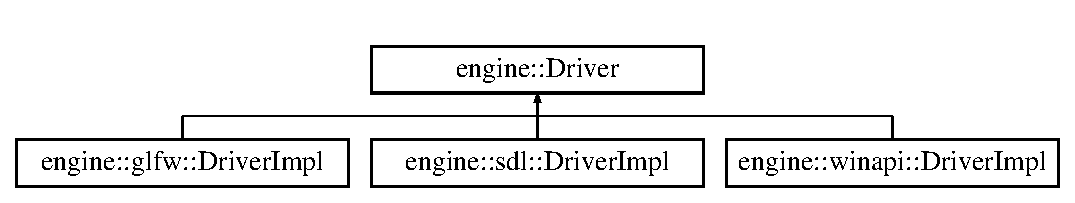
\includegraphics[height=2.000000cm]{a00024}
\end{center}
\end{figure}
\subsubsection*{Public Member Functions}
\begin{DoxyCompactItemize}
\item 
virtual \hyperlink{a00024_a4772e871ef5639c84cbb5569d75c1de9}{$\sim$\+Driver} ()
\item 
void \hyperlink{a00024_a4e283b1274b6ffea595cb7329b09c16d}{init} (const \hyperlink{a00028}{Driver\+Init\+Parameters} \&params, \hyperlink{a00082}{Window} $\ast$window)
\item 
virtual \hyperlink{a00024_a4772e871ef5639c84cbb5569d75c1de9}{$\sim$\+Driver} ()
\item 
void \hyperlink{a00024_a4e283b1274b6ffea595cb7329b09c16d}{init} (const \hyperlink{a00028}{Driver\+Init\+Parameters} \&params, \hyperlink{a00082}{Window} $\ast$window)
\end{DoxyCompactItemize}
\subsubsection*{Protected Member Functions}
\begin{DoxyCompactItemize}
\item 
\hyperlink{a00024_aed71bf52de93e2fc50f12eb860a52acc}{Driver} ()=default
\item 
\hyperlink{a00024_aed71bf52de93e2fc50f12eb860a52acc}{Driver} ()=default
\end{DoxyCompactItemize}
\subsubsection*{Friends}
\begin{DoxyCompactItemize}
\item 
class {\bfseries Window\+Manager}\hypertarget{a00024_a8bf419dae80cc317c90469d0199cfdd5}{}\label{a00024_a8bf419dae80cc317c90469d0199cfdd5}

\item 
struct {\bfseries Window\+Manager\+Private}\hypertarget{a00024_a1e888245e5e110e096f9476dd22b68ec}{}\label{a00024_a1e888245e5e110e096f9476dd22b68ec}

\end{DoxyCompactItemize}


\subsubsection{Detailed Description}


Definition at line 21 of file Driver.\+h.



\subsubsection{Constructor \& Destructor Documentation}
\index{engine\+::\+Driver@{engine\+::\+Driver}!Driver@{Driver}}
\index{Driver@{Driver}!engine\+::\+Driver@{engine\+::\+Driver}}
\paragraph[{\texorpdfstring{Driver()=default}{Driver()=default}}]{\setlength{\rightskip}{0pt plus 5cm}engine\+::\+Driver\+::\+Driver (
\begin{DoxyParamCaption}
{}
\end{DoxyParamCaption}
)\hspace{0.3cm}{\ttfamily [protected]}, {\ttfamily [default]}}\hypertarget{a00024_aed71bf52de93e2fc50f12eb860a52acc}{}\label{a00024_aed71bf52de93e2fc50f12eb860a52acc}
Simple constructor \index{engine\+::\+Driver@{engine\+::\+Driver}!````~Driver@{$\sim$\+Driver}}
\index{````~Driver@{$\sim$\+Driver}!engine\+::\+Driver@{engine\+::\+Driver}}
\paragraph[{\texorpdfstring{$\sim$\+Driver()}{~Driver()}}]{\setlength{\rightskip}{0pt plus 5cm}virtual engine\+::\+Driver\+::$\sim$\+Driver (
\begin{DoxyParamCaption}
{}
\end{DoxyParamCaption}
)\hspace{0.3cm}{\ttfamily [inline]}, {\ttfamily [virtual]}}\hypertarget{a00024_a4772e871ef5639c84cbb5569d75c1de9}{}\label{a00024_a4772e871ef5639c84cbb5569d75c1de9}
Virtual destructor 

Definition at line 31 of file Driver.\+h.

\index{engine\+::\+Driver@{engine\+::\+Driver}!Driver@{Driver}}
\index{Driver@{Driver}!engine\+::\+Driver@{engine\+::\+Driver}}
\paragraph[{\texorpdfstring{Driver()=default}{Driver()=default}}]{\setlength{\rightskip}{0pt plus 5cm}engine\+::\+Driver\+::\+Driver (
\begin{DoxyParamCaption}
{}
\end{DoxyParamCaption}
)\hspace{0.3cm}{\ttfamily [protected]}, {\ttfamily [default]}}\hypertarget{a00024_aed71bf52de93e2fc50f12eb860a52acc}{}\label{a00024_aed71bf52de93e2fc50f12eb860a52acc}
Simple constructor \index{engine\+::\+Driver@{engine\+::\+Driver}!````~Driver@{$\sim$\+Driver}}
\index{````~Driver@{$\sim$\+Driver}!engine\+::\+Driver@{engine\+::\+Driver}}
\paragraph[{\texorpdfstring{$\sim$\+Driver()}{~Driver()}}]{\setlength{\rightskip}{0pt plus 5cm}virtual engine\+::\+Driver\+::$\sim$\+Driver (
\begin{DoxyParamCaption}
{}
\end{DoxyParamCaption}
)\hspace{0.3cm}{\ttfamily [inline]}, {\ttfamily [virtual]}}\hypertarget{a00024_a4772e871ef5639c84cbb5569d75c1de9}{}\label{a00024_a4772e871ef5639c84cbb5569d75c1de9}
Virtual destructor 

Definition at line 31 of file Driver.\+h.



\subsubsection{Member Function Documentation}
\index{engine\+::\+Driver@{engine\+::\+Driver}!init@{init}}
\index{init@{init}!engine\+::\+Driver@{engine\+::\+Driver}}
\paragraph[{\texorpdfstring{init(const Driver\+Init\+Parameters \&params, Window $\ast$window)}{init(const DriverInitParameters &params, Window *window)}}]{\setlength{\rightskip}{0pt plus 5cm}void engine\+::\+Driver\+::init (
\begin{DoxyParamCaption}
\item[{const {\bf Driver\+Init\+Parameters} \&}]{params, }
\item[{{\bf Window} $\ast$}]{window}
\end{DoxyParamCaption}
)}\hypertarget{a00024_a4e283b1274b6ffea595cb7329b09c16d}{}\label{a00024_a4e283b1274b6ffea595cb7329b09c16d}
Init function \index{engine\+::\+Driver@{engine\+::\+Driver}!init@{init}}
\index{init@{init}!engine\+::\+Driver@{engine\+::\+Driver}}
\paragraph[{\texorpdfstring{init(const Driver\+Init\+Parameters \&params, Window $\ast$window)}{init(const DriverInitParameters &params, Window *window)}}]{\setlength{\rightskip}{0pt plus 5cm}void engine\+::\+Driver\+::init (
\begin{DoxyParamCaption}
\item[{const {\bf Driver\+Init\+Parameters} \&}]{params, }
\item[{{\bf Window} $\ast$}]{window}
\end{DoxyParamCaption}
)}\hypertarget{a00024_a4e283b1274b6ffea595cb7329b09c16d}{}\label{a00024_a4e283b1274b6ffea595cb7329b09c16d}
Init function 

The documentation for this class was generated from the following file\+:\begin{DoxyCompactItemize}
\item 
E\+:/\+Programing/\+Projects/\+Engine\+Workspace/\+Common\+Libs/engine/include/engine/video/Driver.\+h\end{DoxyCompactItemize}

\hypertarget{a00025}{}\subsection{engine\+:\+:glfw\+:\+:Driver\+Impl Class Reference}
\label{a00025}\index{engine\+::glfw\+::\+Driver\+Impl@{engine\+::glfw\+::\+Driver\+Impl}}


{\ttfamily \#include $<$E\+:/\+Programing/\+Projects/\+Engine\+Workspace/\+Common\+Libs/engine/include/engine/video/glfw/\+Driver\+Impl.\+h$>$}

Inheritance diagram for engine\+:\+:glfw\+:\+:Driver\+Impl\+:\begin{figure}[H]
\begin{center}
\leavevmode
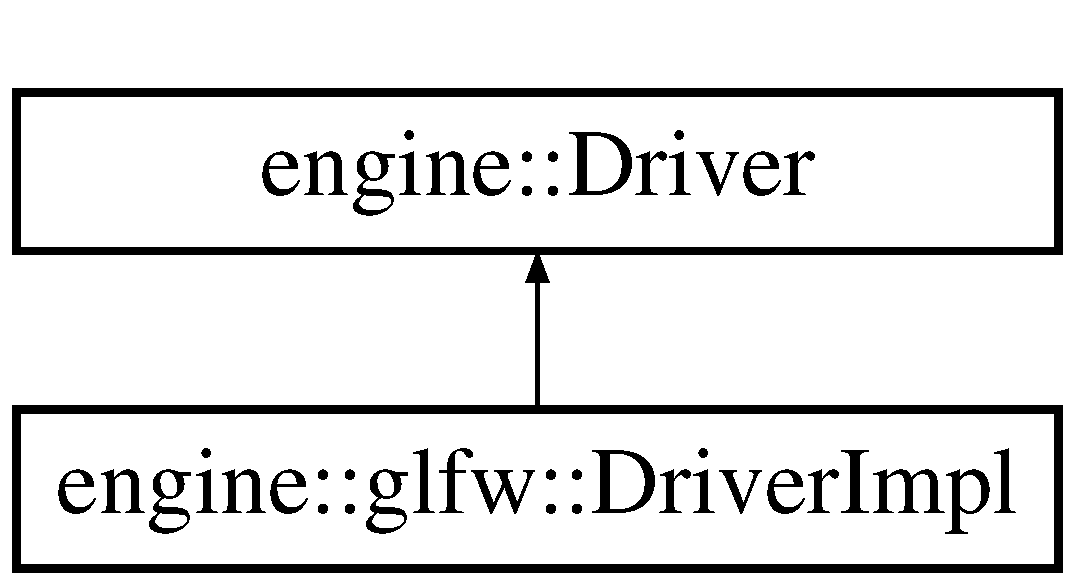
\includegraphics[height=2.000000cm]{a00025}
\end{center}
\end{figure}
\subsubsection*{Public Member Functions}
\begin{DoxyCompactItemize}
\item 
\hyperlink{a00025_a97b0fadb208251c7a998e0a1e2480a67}{Driver\+Impl} ()
\item 
\hyperlink{a00025_a18a74e07839478fede104c56a7ec73a1}{$\sim$\+Driver\+Impl} () override
\item 
void \hyperlink{a00025_ab25927deeb820162e36fe494e6abb357}{init\+Impl} (const \hyperlink{a00028}{Driver\+Init\+Parameters} \&params, \hyperlink{a00082}{Window} $\ast$window) override
\item 
void \hyperlink{a00024_a4e283b1274b6ffea595cb7329b09c16d}{init} (const \hyperlink{a00028}{Driver\+Init\+Parameters} \&params, \hyperlink{a00082}{Window} $\ast$window)
\item 
void \hyperlink{a00024_a4e283b1274b6ffea595cb7329b09c16d}{init} (const \hyperlink{a00028}{Driver\+Init\+Parameters} \&params, \hyperlink{a00082}{Window} $\ast$window)
\end{DoxyCompactItemize}


\subsubsection{Detailed Description}
Video driver implementation for winapi 

Definition at line 12 of file Driver\+Impl.\+h.



\subsubsection{Constructor \& Destructor Documentation}
\index{engine\+::glfw\+::\+Driver\+Impl@{engine\+::glfw\+::\+Driver\+Impl}!Driver\+Impl@{Driver\+Impl}}
\index{Driver\+Impl@{Driver\+Impl}!engine\+::glfw\+::\+Driver\+Impl@{engine\+::glfw\+::\+Driver\+Impl}}
\paragraph[{\texorpdfstring{Driver\+Impl()}{DriverImpl()}}]{\setlength{\rightskip}{0pt plus 5cm}engine\+::glfw\+::\+Driver\+Impl\+::\+Driver\+Impl (
\begin{DoxyParamCaption}
{}
\end{DoxyParamCaption}
)}\hypertarget{a00025_a97b0fadb208251c7a998e0a1e2480a67}{}\label{a00025_a97b0fadb208251c7a998e0a1e2480a67}
Simple constructor \index{engine\+::glfw\+::\+Driver\+Impl@{engine\+::glfw\+::\+Driver\+Impl}!````~Driver\+Impl@{$\sim$\+Driver\+Impl}}
\index{````~Driver\+Impl@{$\sim$\+Driver\+Impl}!engine\+::glfw\+::\+Driver\+Impl@{engine\+::glfw\+::\+Driver\+Impl}}
\paragraph[{\texorpdfstring{$\sim$\+Driver\+Impl() override}{~DriverImpl() override}}]{\setlength{\rightskip}{0pt plus 5cm}engine\+::glfw\+::\+Driver\+Impl\+::$\sim$\+Driver\+Impl (
\begin{DoxyParamCaption}
{}
\end{DoxyParamCaption}
)\hspace{0.3cm}{\ttfamily [override]}}\hypertarget{a00025_a18a74e07839478fede104c56a7ec73a1}{}\label{a00025_a18a74e07839478fede104c56a7ec73a1}
For P\+I\+M\+PL 

\subsubsection{Member Function Documentation}
\index{engine\+::glfw\+::\+Driver\+Impl@{engine\+::glfw\+::\+Driver\+Impl}!init@{init}}
\index{init@{init}!engine\+::glfw\+::\+Driver\+Impl@{engine\+::glfw\+::\+Driver\+Impl}}
\paragraph[{\texorpdfstring{init(const Driver\+Init\+Parameters \&params, Window $\ast$window)}{init(const DriverInitParameters &params, Window *window)}}]{\setlength{\rightskip}{0pt plus 5cm}void engine\+::\+Driver\+::init (
\begin{DoxyParamCaption}
\item[{const {\bf Driver\+Init\+Parameters} \&}]{params, }
\item[{{\bf Window} $\ast$}]{window}
\end{DoxyParamCaption}
)\hspace{0.3cm}{\ttfamily [inherited]}}\hypertarget{a00024_a4e283b1274b6ffea595cb7329b09c16d}{}\label{a00024_a4e283b1274b6ffea595cb7329b09c16d}
Init function \index{engine\+::glfw\+::\+Driver\+Impl@{engine\+::glfw\+::\+Driver\+Impl}!init@{init}}
\index{init@{init}!engine\+::glfw\+::\+Driver\+Impl@{engine\+::glfw\+::\+Driver\+Impl}}
\paragraph[{\texorpdfstring{init(const Driver\+Init\+Parameters \&params, Window $\ast$window)}{init(const DriverInitParameters &params, Window *window)}}]{\setlength{\rightskip}{0pt plus 5cm}void engine\+::\+Driver\+::init (
\begin{DoxyParamCaption}
\item[{const {\bf Driver\+Init\+Parameters} \&}]{params, }
\item[{{\bf Window} $\ast$}]{window}
\end{DoxyParamCaption}
)\hspace{0.3cm}{\ttfamily [inherited]}}\hypertarget{a00024_a4e283b1274b6ffea595cb7329b09c16d}{}\label{a00024_a4e283b1274b6ffea595cb7329b09c16d}
Init function \index{engine\+::glfw\+::\+Driver\+Impl@{engine\+::glfw\+::\+Driver\+Impl}!init\+Impl@{init\+Impl}}
\index{init\+Impl@{init\+Impl}!engine\+::glfw\+::\+Driver\+Impl@{engine\+::glfw\+::\+Driver\+Impl}}
\paragraph[{\texorpdfstring{init\+Impl(const Driver\+Init\+Parameters \&params, Window $\ast$window) override}{initImpl(const DriverInitParameters &params, Window *window) override}}]{\setlength{\rightskip}{0pt plus 5cm}void engine\+::glfw\+::\+Driver\+Impl\+::init\+Impl (
\begin{DoxyParamCaption}
\item[{const {\bf Driver\+Init\+Parameters} \&}]{params, }
\item[{{\bf Window} $\ast$}]{window}
\end{DoxyParamCaption}
)\hspace{0.3cm}{\ttfamily [override]}, {\ttfamily [virtual]}}\hypertarget{a00025_ab25927deeb820162e36fe494e6abb357}{}\label{a00025_ab25927deeb820162e36fe494e6abb357}
Initialize based on the given window 

Implements \hyperlink{a00024}{engine\+::\+Driver}.



The documentation for this class was generated from the following file\+:\begin{DoxyCompactItemize}
\item 
E\+:/\+Programing/\+Projects/\+Engine\+Workspace/\+Common\+Libs/engine/include/engine/video/glfw/Driver\+Impl.\+h\end{DoxyCompactItemize}

\hypertarget{a00026}{}\subsection{engine\+:\+:sdl\+:\+:Driver\+Impl Class Reference}
\label{a00026}\index{engine\+::sdl\+::\+Driver\+Impl@{engine\+::sdl\+::\+Driver\+Impl}}


{\ttfamily \#include $<$E\+:/\+Programing/\+Projects/\+Engine\+Workspace/\+Common\+Libs/engine/include/engine/video/sdl/\+Driver\+Impl.\+h$>$}

Inheritance diagram for engine\+:\+:sdl\+:\+:Driver\+Impl\+:\begin{figure}[H]
\begin{center}
\leavevmode
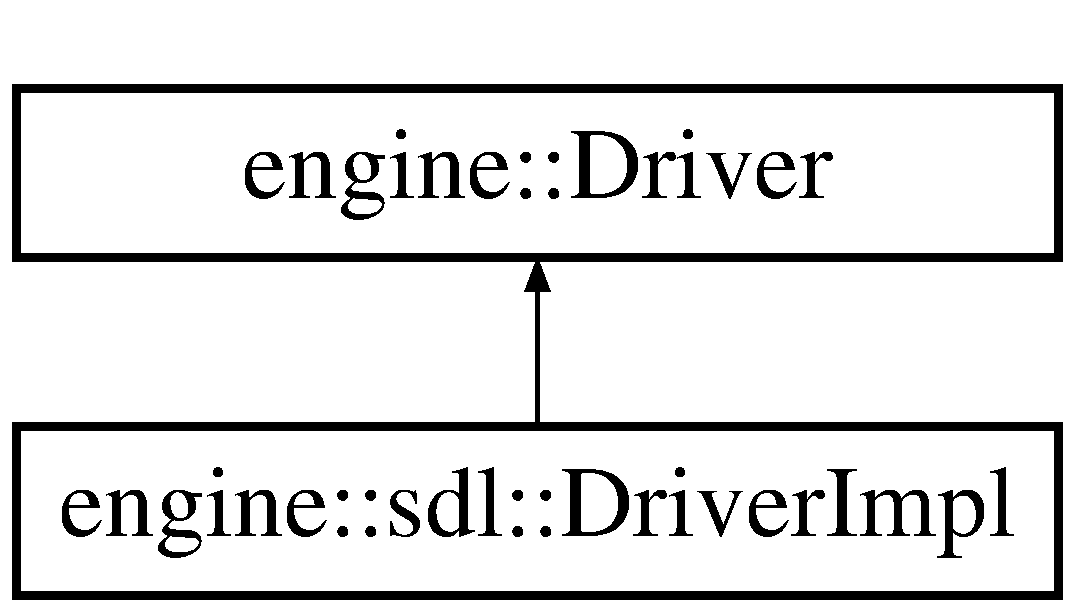
\includegraphics[height=2.000000cm]{a00026}
\end{center}
\end{figure}
\subsubsection*{Public Member Functions}
\begin{DoxyCompactItemize}
\item 
\hyperlink{a00026_a0a1b946eea9e2d648d98be26caeb2c60}{Driver\+Impl} ()
\item 
\hyperlink{a00026_afc245b5c1c99e8b5d73e14c52239e319}{$\sim$\+Driver\+Impl} () override
\item 
void \hyperlink{a00026_a831cf6d2ef096f515727d23f19ab9d41}{init\+Impl} (const \hyperlink{a00028}{Driver\+Init\+Parameters} \&params, \hyperlink{a00082}{Window} $\ast$window) override
\item 
void \hyperlink{a00024_a4e283b1274b6ffea595cb7329b09c16d}{init} (const \hyperlink{a00028}{Driver\+Init\+Parameters} \&params, \hyperlink{a00082}{Window} $\ast$window)
\item 
void \hyperlink{a00024_a4e283b1274b6ffea595cb7329b09c16d}{init} (const \hyperlink{a00028}{Driver\+Init\+Parameters} \&params, \hyperlink{a00082}{Window} $\ast$window)
\end{DoxyCompactItemize}


\subsubsection{Detailed Description}
Video driver implementation for winapi 

Definition at line 12 of file Driver\+Impl.\+h.



\subsubsection{Constructor \& Destructor Documentation}
\index{engine\+::sdl\+::\+Driver\+Impl@{engine\+::sdl\+::\+Driver\+Impl}!Driver\+Impl@{Driver\+Impl}}
\index{Driver\+Impl@{Driver\+Impl}!engine\+::sdl\+::\+Driver\+Impl@{engine\+::sdl\+::\+Driver\+Impl}}
\paragraph[{\texorpdfstring{Driver\+Impl()}{DriverImpl()}}]{\setlength{\rightskip}{0pt plus 5cm}engine\+::sdl\+::\+Driver\+Impl\+::\+Driver\+Impl (
\begin{DoxyParamCaption}
{}
\end{DoxyParamCaption}
)}\hypertarget{a00026_a0a1b946eea9e2d648d98be26caeb2c60}{}\label{a00026_a0a1b946eea9e2d648d98be26caeb2c60}
Simple constructor \index{engine\+::sdl\+::\+Driver\+Impl@{engine\+::sdl\+::\+Driver\+Impl}!````~Driver\+Impl@{$\sim$\+Driver\+Impl}}
\index{````~Driver\+Impl@{$\sim$\+Driver\+Impl}!engine\+::sdl\+::\+Driver\+Impl@{engine\+::sdl\+::\+Driver\+Impl}}
\paragraph[{\texorpdfstring{$\sim$\+Driver\+Impl() override}{~DriverImpl() override}}]{\setlength{\rightskip}{0pt plus 5cm}engine\+::sdl\+::\+Driver\+Impl\+::$\sim$\+Driver\+Impl (
\begin{DoxyParamCaption}
{}
\end{DoxyParamCaption}
)\hspace{0.3cm}{\ttfamily [override]}}\hypertarget{a00026_afc245b5c1c99e8b5d73e14c52239e319}{}\label{a00026_afc245b5c1c99e8b5d73e14c52239e319}
For P\+I\+M\+PL 

\subsubsection{Member Function Documentation}
\index{engine\+::sdl\+::\+Driver\+Impl@{engine\+::sdl\+::\+Driver\+Impl}!init@{init}}
\index{init@{init}!engine\+::sdl\+::\+Driver\+Impl@{engine\+::sdl\+::\+Driver\+Impl}}
\paragraph[{\texorpdfstring{init(const Driver\+Init\+Parameters \&params, Window $\ast$window)}{init(const DriverInitParameters &params, Window *window)}}]{\setlength{\rightskip}{0pt plus 5cm}void engine\+::\+Driver\+::init (
\begin{DoxyParamCaption}
\item[{const {\bf Driver\+Init\+Parameters} \&}]{params, }
\item[{{\bf Window} $\ast$}]{window}
\end{DoxyParamCaption}
)\hspace{0.3cm}{\ttfamily [inherited]}}\hypertarget{a00024_a4e283b1274b6ffea595cb7329b09c16d}{}\label{a00024_a4e283b1274b6ffea595cb7329b09c16d}
Init function \index{engine\+::sdl\+::\+Driver\+Impl@{engine\+::sdl\+::\+Driver\+Impl}!init@{init}}
\index{init@{init}!engine\+::sdl\+::\+Driver\+Impl@{engine\+::sdl\+::\+Driver\+Impl}}
\paragraph[{\texorpdfstring{init(const Driver\+Init\+Parameters \&params, Window $\ast$window)}{init(const DriverInitParameters &params, Window *window)}}]{\setlength{\rightskip}{0pt plus 5cm}void engine\+::\+Driver\+::init (
\begin{DoxyParamCaption}
\item[{const {\bf Driver\+Init\+Parameters} \&}]{params, }
\item[{{\bf Window} $\ast$}]{window}
\end{DoxyParamCaption}
)\hspace{0.3cm}{\ttfamily [inherited]}}\hypertarget{a00024_a4e283b1274b6ffea595cb7329b09c16d}{}\label{a00024_a4e283b1274b6ffea595cb7329b09c16d}
Init function \index{engine\+::sdl\+::\+Driver\+Impl@{engine\+::sdl\+::\+Driver\+Impl}!init\+Impl@{init\+Impl}}
\index{init\+Impl@{init\+Impl}!engine\+::sdl\+::\+Driver\+Impl@{engine\+::sdl\+::\+Driver\+Impl}}
\paragraph[{\texorpdfstring{init\+Impl(const Driver\+Init\+Parameters \&params, Window $\ast$window) override}{initImpl(const DriverInitParameters &params, Window *window) override}}]{\setlength{\rightskip}{0pt plus 5cm}void engine\+::sdl\+::\+Driver\+Impl\+::init\+Impl (
\begin{DoxyParamCaption}
\item[{const {\bf Driver\+Init\+Parameters} \&}]{params, }
\item[{{\bf Window} $\ast$}]{window}
\end{DoxyParamCaption}
)\hspace{0.3cm}{\ttfamily [override]}, {\ttfamily [virtual]}}\hypertarget{a00026_a831cf6d2ef096f515727d23f19ab9d41}{}\label{a00026_a831cf6d2ef096f515727d23f19ab9d41}
Initialize based on the given window 

Implements \hyperlink{a00024}{engine\+::\+Driver}.



The documentation for this class was generated from the following file\+:\begin{DoxyCompactItemize}
\item 
E\+:/\+Programing/\+Projects/\+Engine\+Workspace/\+Common\+Libs/engine/include/engine/video/sdl/Driver\+Impl.\+h\end{DoxyCompactItemize}

\hypertarget{a00027}{}\subsection{engine\+:\+:winapi\+:\+:Driver\+Impl Class Reference}
\label{a00027}\index{engine\+::winapi\+::\+Driver\+Impl@{engine\+::winapi\+::\+Driver\+Impl}}


{\ttfamily \#include $<$E\+:/\+Programing/\+Projects/\+Engine\+Workspace/\+Common\+Libs/engine/include/engine/video/winapi/\+Driver\+Impl.\+h$>$}

Inheritance diagram for engine\+:\+:winapi\+:\+:Driver\+Impl\+:\begin{figure}[H]
\begin{center}
\leavevmode
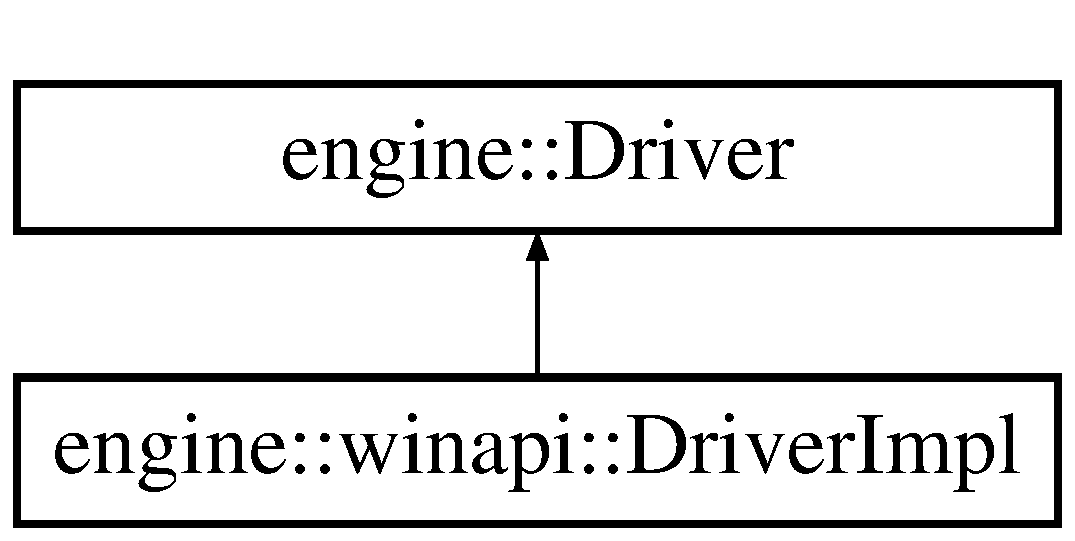
\includegraphics[height=2.000000cm]{a00027}
\end{center}
\end{figure}
\subsubsection*{Public Member Functions}
\begin{DoxyCompactItemize}
\item 
\hyperlink{a00027_a5819d40195dd4ecc23de16090c20f746}{Driver\+Impl} ()
\item 
\hyperlink{a00027_a700cf49e15416ea10fc567459535f9f1}{$\sim$\+Driver\+Impl} () override
\item 
void \hyperlink{a00027_a1a6bbae98bc32e3c78c0a47092bda76a}{init\+Impl} (const \hyperlink{a00028}{Driver\+Init\+Parameters} \&params, \hyperlink{a00082}{Window} $\ast$window) override
\item 
void \hyperlink{a00024_a4e283b1274b6ffea595cb7329b09c16d}{init} (const \hyperlink{a00028}{Driver\+Init\+Parameters} \&params, \hyperlink{a00082}{Window} $\ast$window)
\item 
void \hyperlink{a00024_a4e283b1274b6ffea595cb7329b09c16d}{init} (const \hyperlink{a00028}{Driver\+Init\+Parameters} \&params, \hyperlink{a00082}{Window} $\ast$window)
\end{DoxyCompactItemize}


\subsubsection{Detailed Description}
Video driver implementation for winapi 

Definition at line 12 of file Driver\+Impl.\+h.



\subsubsection{Constructor \& Destructor Documentation}
\index{engine\+::winapi\+::\+Driver\+Impl@{engine\+::winapi\+::\+Driver\+Impl}!Driver\+Impl@{Driver\+Impl}}
\index{Driver\+Impl@{Driver\+Impl}!engine\+::winapi\+::\+Driver\+Impl@{engine\+::winapi\+::\+Driver\+Impl}}
\paragraph[{\texorpdfstring{Driver\+Impl()}{DriverImpl()}}]{\setlength{\rightskip}{0pt plus 5cm}engine\+::winapi\+::\+Driver\+Impl\+::\+Driver\+Impl (
\begin{DoxyParamCaption}
{}
\end{DoxyParamCaption}
)}\hypertarget{a00027_a5819d40195dd4ecc23de16090c20f746}{}\label{a00027_a5819d40195dd4ecc23de16090c20f746}
Simple constructor \index{engine\+::winapi\+::\+Driver\+Impl@{engine\+::winapi\+::\+Driver\+Impl}!````~Driver\+Impl@{$\sim$\+Driver\+Impl}}
\index{````~Driver\+Impl@{$\sim$\+Driver\+Impl}!engine\+::winapi\+::\+Driver\+Impl@{engine\+::winapi\+::\+Driver\+Impl}}
\paragraph[{\texorpdfstring{$\sim$\+Driver\+Impl() override}{~DriverImpl() override}}]{\setlength{\rightskip}{0pt plus 5cm}engine\+::winapi\+::\+Driver\+Impl\+::$\sim$\+Driver\+Impl (
\begin{DoxyParamCaption}
{}
\end{DoxyParamCaption}
)\hspace{0.3cm}{\ttfamily [override]}}\hypertarget{a00027_a700cf49e15416ea10fc567459535f9f1}{}\label{a00027_a700cf49e15416ea10fc567459535f9f1}
For P\+I\+M\+PL 

\subsubsection{Member Function Documentation}
\index{engine\+::winapi\+::\+Driver\+Impl@{engine\+::winapi\+::\+Driver\+Impl}!init@{init}}
\index{init@{init}!engine\+::winapi\+::\+Driver\+Impl@{engine\+::winapi\+::\+Driver\+Impl}}
\paragraph[{\texorpdfstring{init(const Driver\+Init\+Parameters \&params, Window $\ast$window)}{init(const DriverInitParameters &params, Window *window)}}]{\setlength{\rightskip}{0pt plus 5cm}void engine\+::\+Driver\+::init (
\begin{DoxyParamCaption}
\item[{const {\bf Driver\+Init\+Parameters} \&}]{params, }
\item[{{\bf Window} $\ast$}]{window}
\end{DoxyParamCaption}
)\hspace{0.3cm}{\ttfamily [inherited]}}\hypertarget{a00024_a4e283b1274b6ffea595cb7329b09c16d}{}\label{a00024_a4e283b1274b6ffea595cb7329b09c16d}
Init function \index{engine\+::winapi\+::\+Driver\+Impl@{engine\+::winapi\+::\+Driver\+Impl}!init@{init}}
\index{init@{init}!engine\+::winapi\+::\+Driver\+Impl@{engine\+::winapi\+::\+Driver\+Impl}}
\paragraph[{\texorpdfstring{init(const Driver\+Init\+Parameters \&params, Window $\ast$window)}{init(const DriverInitParameters &params, Window *window)}}]{\setlength{\rightskip}{0pt plus 5cm}void engine\+::\+Driver\+::init (
\begin{DoxyParamCaption}
\item[{const {\bf Driver\+Init\+Parameters} \&}]{params, }
\item[{{\bf Window} $\ast$}]{window}
\end{DoxyParamCaption}
)\hspace{0.3cm}{\ttfamily [inherited]}}\hypertarget{a00024_a4e283b1274b6ffea595cb7329b09c16d}{}\label{a00024_a4e283b1274b6ffea595cb7329b09c16d}
Init function \index{engine\+::winapi\+::\+Driver\+Impl@{engine\+::winapi\+::\+Driver\+Impl}!init\+Impl@{init\+Impl}}
\index{init\+Impl@{init\+Impl}!engine\+::winapi\+::\+Driver\+Impl@{engine\+::winapi\+::\+Driver\+Impl}}
\paragraph[{\texorpdfstring{init\+Impl(const Driver\+Init\+Parameters \&params, Window $\ast$window) override}{initImpl(const DriverInitParameters &params, Window *window) override}}]{\setlength{\rightskip}{0pt plus 5cm}void engine\+::winapi\+::\+Driver\+Impl\+::init\+Impl (
\begin{DoxyParamCaption}
\item[{const {\bf Driver\+Init\+Parameters} \&}]{params, }
\item[{{\bf Window} $\ast$}]{window}
\end{DoxyParamCaption}
)\hspace{0.3cm}{\ttfamily [override]}, {\ttfamily [virtual]}}\hypertarget{a00027_a1a6bbae98bc32e3c78c0a47092bda76a}{}\label{a00027_a1a6bbae98bc32e3c78c0a47092bda76a}
Initialize based on the given window 

Implements \hyperlink{a00024}{engine\+::\+Driver}.



The documentation for this class was generated from the following file\+:\begin{DoxyCompactItemize}
\item 
E\+:/\+Programing/\+Projects/\+Engine\+Workspace/\+Common\+Libs/engine/include/engine/video/winapi/Driver\+Impl.\+h\end{DoxyCompactItemize}

\hypertarget{a00028}{}\subsection{engine\+:\+:Driver\+Init\+Parameters Struct Reference}
\label{a00028}\index{engine\+::\+Driver\+Init\+Parameters@{engine\+::\+Driver\+Init\+Parameters}}


{\ttfamily \#include $<$E\+:/\+Programing/\+Projects/\+Engine\+Workspace/\+Common\+Libs/engine/include/engine/video/\+Driver.\+h$>$}

\subsubsection*{Public Attributes}
\begin{DoxyCompactItemize}
\item 
\hyperlink{a00007}{Buffer\+Desc} \hyperlink{a00028_a3c2e3a43440396f00417f098628c6649}{description}
\item 
int32\+\_\+t \hyperlink{a00028_afab1afded563f9ab42273f7993cdf3ed}{sample\+Count}
\end{DoxyCompactItemize}


\subsubsection{Detailed Description}
Initialization parameters for the driver 

Definition at line 13 of file Driver.\+h.



\subsubsection{Member Data Documentation}
\index{engine\+::\+Driver\+Init\+Parameters@{engine\+::\+Driver\+Init\+Parameters}!description@{description}}
\index{description@{description}!engine\+::\+Driver\+Init\+Parameters@{engine\+::\+Driver\+Init\+Parameters}}
\paragraph[{\texorpdfstring{description}{description}}]{\setlength{\rightskip}{0pt plus 5cm}{\bf Buffer\+Desc} engine\+::\+Driver\+Init\+Parameters\+::description}\hypertarget{a00028_a3c2e3a43440396f00417f098628c6649}{}\label{a00028_a3c2e3a43440396f00417f098628c6649}
Buffer descripition of the main buffer 

Definition at line 16 of file Driver.\+h.

\index{engine\+::\+Driver\+Init\+Parameters@{engine\+::\+Driver\+Init\+Parameters}!sample\+Count@{sample\+Count}}
\index{sample\+Count@{sample\+Count}!engine\+::\+Driver\+Init\+Parameters@{engine\+::\+Driver\+Init\+Parameters}}
\paragraph[{\texorpdfstring{sample\+Count}{sampleCount}}]{\setlength{\rightskip}{0pt plus 5cm}int32\+\_\+t engine\+::\+Driver\+Init\+Parameters\+::sample\+Count}\hypertarget{a00028_afab1afded563f9ab42273f7993cdf3ed}{}\label{a00028_afab1afded563f9ab42273f7993cdf3ed}
Sample count of the driver 

Definition at line 18 of file Driver.\+h.



The documentation for this struct was generated from the following file\+:\begin{DoxyCompactItemize}
\item 
E\+:/\+Programing/\+Projects/\+Engine\+Workspace/\+Common\+Libs/engine/include/engine/video/Driver.\+h\end{DoxyCompactItemize}

\hypertarget{a00029}{}\subsection{engine\+:\+:Easy\+Builder Class Reference}
\label{a00029}\index{engine\+::\+Easy\+Builder@{engine\+::\+Easy\+Builder}}
Inheritance diagram for engine\+:\+:Easy\+Builder\+:\begin{figure}[H]
\begin{center}
\leavevmode
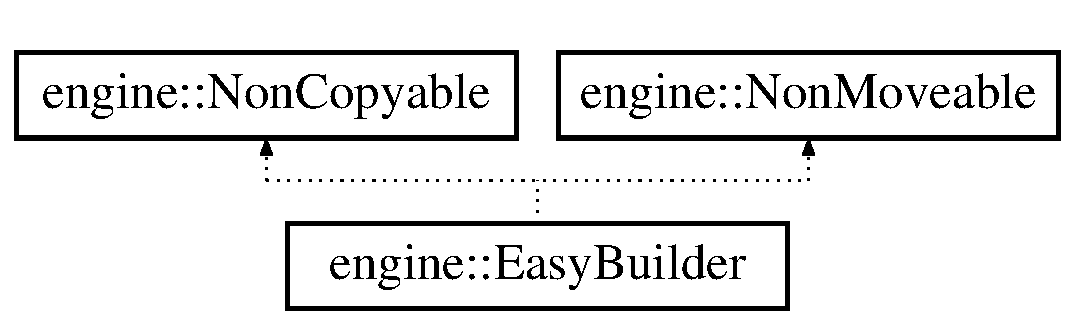
\includegraphics[height=2.000000cm]{a00029}
\end{center}
\end{figure}
\subsubsection*{Public Member Functions}
\begin{DoxyCompactItemize}
\item 
{\bfseries Easy\+Builder} (std\+::unique\+\_\+ptr$<$ \hyperlink{a00045}{I\+Main} $>$ \&\&main)\hypertarget{a00029_a09b7e48d58c0867f7fa32fbc72f50b31}{}\label{a00029_a09b7e48d58c0867f7fa32fbc72f50b31}

\item 
\hyperlink{a00029}{Easy\+Builder} \& {\bfseries Add\+Input} (engine\+::\+Event\+Builder\+::\+Basic\+Input\+Type)\hypertarget{a00029_a8f38c9e1b46fa80982e4d779509ac93d}{}\label{a00029_a8f38c9e1b46fa80982e4d779509ac93d}

\item 
\hyperlink{a00002}{Application} $\ast$ {\bfseries build\+Engine} (H\+I\+N\+S\+T\+A\+N\+CE h\+Instance, H\+I\+N\+S\+T\+A\+N\+CE h\+Prev\+Instance, L\+P\+S\+TR lp\+Cmd\+Line, int n\+Cmd\+Show) const \hypertarget{a00029_adeeb5a7c09d1e05689ed6325282130d4}{}\label{a00029_adeeb5a7c09d1e05689ed6325282130d4}

\item 
\hyperlink{a00002}{Application} $\ast$ {\bfseries build\+Engine} (int argc, char $\ast$argv\mbox{[}$\,$\mbox{]}) const \hypertarget{a00029_a26beb6a3b5e9176bccd0c54149efb200}{}\label{a00029_a26beb6a3b5e9176bccd0c54149efb200}

\end{DoxyCompactItemize}


\subsubsection{Detailed Description}


Definition at line 13 of file Easy\+Builder.\+h.



The documentation for this class was generated from the following file\+:\begin{DoxyCompactItemize}
\item 
E\+:/\+Programing/\+Projects/\+Engine\+Workspace/\+Common\+Libs/engine/include/engine/environment\+Builder/Easy\+Builder.\+h\end{DoxyCompactItemize}

\hypertarget{a00030}{}\subsection{engine\+:\+:Equal\+To$<$ T $>$ Struct Template Reference}
\label{a00030}\index{engine\+::\+Equal\+To$<$ T $>$@{engine\+::\+Equal\+To$<$ T $>$}}


{\ttfamily \#include $<$E\+:/\+Programing/\+Projects/\+Engine\+Workspace/\+Common\+Libs/engine/include/engine/functional/functions.\+h$>$}

\subsubsection*{Public Member Functions}
\begin{DoxyCompactItemize}
\item 
\hyperlink{a00030_a6f4b19b5863bd40d6c3e424728e5e840}{Equal\+To} (const T \&v)
\item 
bool \hyperlink{a00030_a647e825983c17aac5428bd7f2847c7da}{operator()} (const T \&o)
\end{DoxyCompactItemize}


\subsubsection{Detailed Description}
\subsubsection*{template$<$typename T$>$\\*
struct engine\+::\+Equal\+To$<$ T $>$}

Functional for equality check in standard algorithms. 

Definition at line 9 of file functions.\+h.



\subsubsection{Constructor \& Destructor Documentation}
\index{engine\+::\+Equal\+To@{engine\+::\+Equal\+To}!Equal\+To@{Equal\+To}}
\index{Equal\+To@{Equal\+To}!engine\+::\+Equal\+To@{engine\+::\+Equal\+To}}
\paragraph[{\texorpdfstring{Equal\+To(const T \&v)}{EqualTo(const T &v)}}]{\setlength{\rightskip}{0pt plus 5cm}template$<$typename T $>$ {\bf engine\+::\+Equal\+To}$<$ T $>$\+::{\bf Equal\+To} (
\begin{DoxyParamCaption}
\item[{const T \&}]{v}
\end{DoxyParamCaption}
)\hspace{0.3cm}{\ttfamily [inline]}, {\ttfamily [explicit]}}\hypertarget{a00030_a6f4b19b5863bd40d6c3e424728e5e840}{}\label{a00030_a6f4b19b5863bd40d6c3e424728e5e840}
Create the function from the given value to check. 
\begin{DoxyParams}{Parameters}
{\em v} & value to check the equality \\
\hline
\end{DoxyParams}


Definition at line 15 of file functions.\+h.



\subsubsection{Member Function Documentation}
\index{engine\+::\+Equal\+To@{engine\+::\+Equal\+To}!operator()@{operator()}}
\index{operator()@{operator()}!engine\+::\+Equal\+To@{engine\+::\+Equal\+To}}
\paragraph[{\texorpdfstring{operator()(const T \&o)}{operator()(const T &o)}}]{\setlength{\rightskip}{0pt plus 5cm}template$<$typename T $>$ bool {\bf engine\+::\+Equal\+To}$<$ T $>$\+::operator() (
\begin{DoxyParamCaption}
\item[{const T \&}]{o}
\end{DoxyParamCaption}
)\hspace{0.3cm}{\ttfamily [inline]}}\hypertarget{a00030_a647e825983c17aac5428bd7f2847c7da}{}\label{a00030_a647e825983c17aac5428bd7f2847c7da}
Check whether the given object equals to our one. 
\begin{DoxyParams}{Parameters}
{\em o} & object to check whether equals to the stored value. \\
\hline
\end{DoxyParams}
\begin{DoxyReturn}{Returns}
Returns true if the given object equals to the stored one. 
\end{DoxyReturn}


Definition at line 22 of file functions.\+h.



The documentation for this struct was generated from the following file\+:\begin{DoxyCompactItemize}
\item 
E\+:/\+Programing/\+Projects/\+Engine\+Workspace/\+Common\+Libs/engine/include/engine/functional/functions.\+h\end{DoxyCompactItemize}

\hypertarget{a00031}{}\subsection{engine\+:\+:Event\+Builder Class Reference}
\label{a00031}\index{engine\+::\+Event\+Builder@{engine\+::\+Event\+Builder}}
Inheritance diagram for engine\+:\+:Event\+Builder\+:\begin{figure}[H]
\begin{center}
\leavevmode
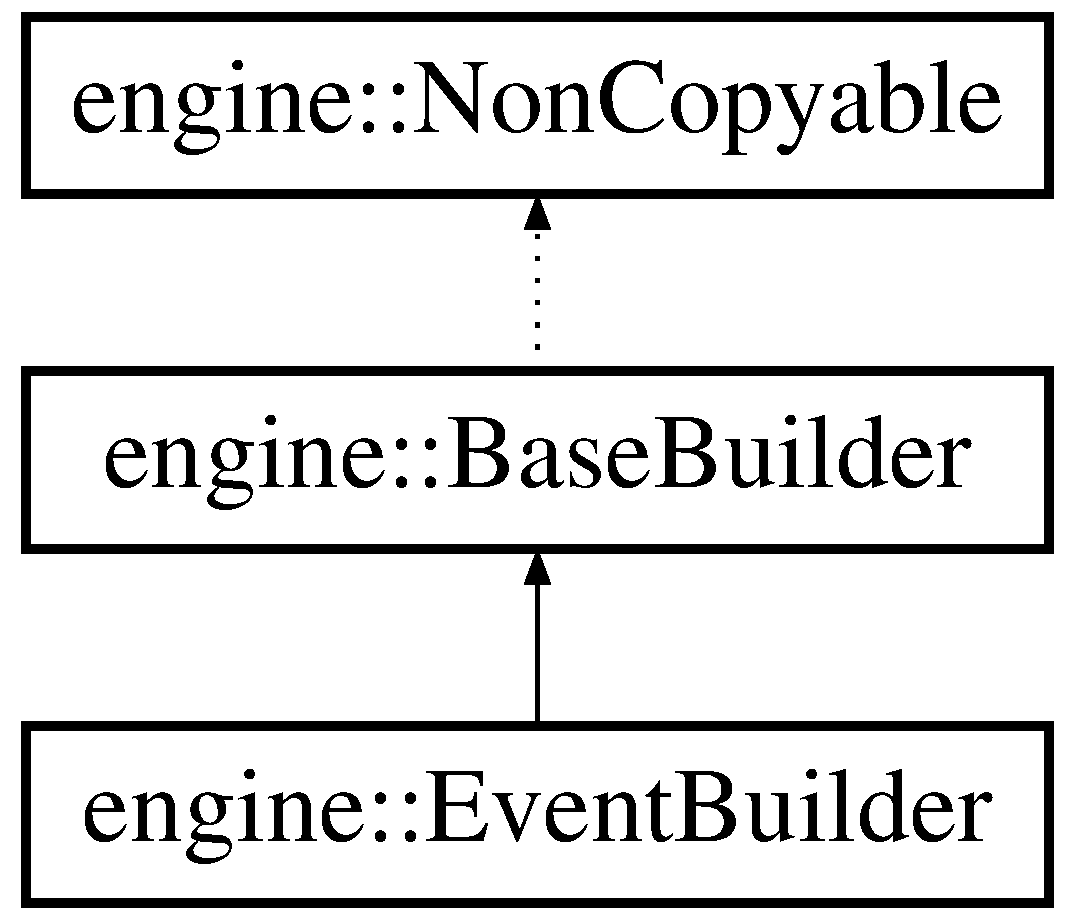
\includegraphics[height=3.000000cm]{a00031}
\end{center}
\end{figure}
\subsubsection*{Public Types}
\begin{DoxyCompactItemize}
\item 
enum {\bfseries Basic\+Input\+Type} \{ {\bfseries Mouse}, 
{\bfseries Keyboard}
 \}\hypertarget{a00031_a6d136f2bc5e63ae4dc52882adcb48ab1}{}\label{a00031_a6d136f2bc5e63ae4dc52882adcb48ab1}

\end{DoxyCompactItemize}
\subsubsection*{Public Member Functions}
\begin{DoxyCompactItemize}
\item 
{\bfseries Event\+Builder} (\hyperlink{a00031}{Event\+Builder} \&\&event\+Builder)\hypertarget{a00031_a26eb2a8a814a70579f1ca30d245b2677}{}\label{a00031_a26eb2a8a814a70579f1ca30d245b2677}

\item 
\hyperlink{a00083}{Window\+Environment\+Builder} {\bfseries build} (const std\+::set$<$ Basic\+Input\+Type $>$ \&basic\+Inputs)\hypertarget{a00031_af77f14d7c5ff0be93dda1520f3441096}{}\label{a00031_af77f14d7c5ff0be93dda1520f3441096}

\item 
\hyperlink{a00083}{Window\+Environment\+Builder} {\bfseries skip} ()\hypertarget{a00031_a0c6c7712c1057dcb7e07a5aecfca5841}{}\label{a00031_a0c6c7712c1057dcb7e07a5aecfca5841}

\end{DoxyCompactItemize}
\subsubsection*{Protected Member Functions}
\begin{DoxyCompactItemize}
\item 
void \hyperlink{a00005_a52fb449fadc5d3a074e3fc7bfb56744b}{add\+Module} (const Context\+Module\+Type value)
\item 
void \hyperlink{a00005_a20c5dafa6892142bc352c13a5f3ac09a}{set\+Application} (std\+::unique\+\_\+ptr$<$ \hyperlink{a00002}{Application} $>$ app)
\item 
void \hyperlink{a00005_a641fb06484bdb07220f445f14db8c0e7}{set\+Window\+Manager} (std\+::unique\+\_\+ptr$<$ \hyperlink{a00087}{Window\+Manager} $>$ manager)
\item 
void \hyperlink{a00005_a52b490a3ef4d2a5b5b7e8e0f82d9a27c}{set\+Event\+Manager} (std\+::unique\+\_\+ptr$<$ \hyperlink{a00034}{Event\+Manager} $>$ manager)
\item 
void \hyperlink{a00005_af23e3bdfb30ca9f2076cacc9029d96c2}{set\+Initialized} ()
\end{DoxyCompactItemize}
\subsubsection*{Friends}
\begin{DoxyCompactItemize}
\item 
class {\bfseries Application\+Builder}\hypertarget{a00031_a8e3ef43d04dac530c01036fa6964e0f6}{}\label{a00031_a8e3ef43d04dac530c01036fa6964e0f6}

\end{DoxyCompactItemize}


\subsubsection{Detailed Description}


Definition at line 14 of file Event\+Builder.\+h.



\subsubsection{Member Function Documentation}
\index{engine\+::\+Event\+Builder@{engine\+::\+Event\+Builder}!add\+Module@{add\+Module}}
\index{add\+Module@{add\+Module}!engine\+::\+Event\+Builder@{engine\+::\+Event\+Builder}}
\paragraph[{\texorpdfstring{add\+Module(const Context\+Module\+Type value)}{addModule(const ContextModuleType value)}}]{\setlength{\rightskip}{0pt plus 5cm}void engine\+::\+Base\+Builder\+::add\+Module (
\begin{DoxyParamCaption}
\item[{const Context\+Module\+Type}]{value}
\end{DoxyParamCaption}
)\hspace{0.3cm}{\ttfamily [protected]}, {\ttfamily [inherited]}}\hypertarget{a00005_a52fb449fadc5d3a074e3fc7bfb56744b}{}\label{a00005_a52fb449fadc5d3a074e3fc7bfb56744b}
Add a module type which is initialized during build phase 
\begin{DoxyParams}{Parameters}
{\em value} & Module which is initialized successfully \\
\hline
\end{DoxyParams}


Referenced by engine\+::\+Base\+Builder\+::$\sim$\+Base\+Builder().

\index{engine\+::\+Event\+Builder@{engine\+::\+Event\+Builder}!set\+Application@{set\+Application}}
\index{set\+Application@{set\+Application}!engine\+::\+Event\+Builder@{engine\+::\+Event\+Builder}}
\paragraph[{\texorpdfstring{set\+Application(std\+::unique\+\_\+ptr$<$ Application $>$ app)}{setApplication(std::unique_ptr< Application > app)}}]{\setlength{\rightskip}{0pt plus 5cm}void engine\+::\+Base\+Builder\+::set\+Application (
\begin{DoxyParamCaption}
\item[{std\+::unique\+\_\+ptr$<$ {\bf Application} $>$}]{app}
\end{DoxyParamCaption}
)\hspace{0.3cm}{\ttfamily [protected]}, {\ttfamily [inherited]}}\hypertarget{a00005_a20c5dafa6892142bc352c13a5f3ac09a}{}\label{a00005_a20c5dafa6892142bc352c13a5f3ac09a}
Set the context application. 
\begin{DoxyParams}{Parameters}
{\em app} & \hyperlink{a00002}{Application} to use \\
\hline
\end{DoxyParams}


Referenced by engine\+::\+Base\+Builder\+::$\sim$\+Base\+Builder().

\index{engine\+::\+Event\+Builder@{engine\+::\+Event\+Builder}!set\+Event\+Manager@{set\+Event\+Manager}}
\index{set\+Event\+Manager@{set\+Event\+Manager}!engine\+::\+Event\+Builder@{engine\+::\+Event\+Builder}}
\paragraph[{\texorpdfstring{set\+Event\+Manager(std\+::unique\+\_\+ptr$<$ Event\+Manager $>$ manager)}{setEventManager(std::unique_ptr< EventManager > manager)}}]{\setlength{\rightskip}{0pt plus 5cm}void engine\+::\+Base\+Builder\+::set\+Event\+Manager (
\begin{DoxyParamCaption}
\item[{std\+::unique\+\_\+ptr$<$ {\bf Event\+Manager} $>$}]{manager}
\end{DoxyParamCaption}
)\hspace{0.3cm}{\ttfamily [protected]}, {\ttfamily [inherited]}}\hypertarget{a00005_a52b490a3ef4d2a5b5b7e8e0f82d9a27c}{}\label{a00005_a52b490a3ef4d2a5b5b7e8e0f82d9a27c}
Set the event manager of the context. 
\begin{DoxyParams}{Parameters}
{\em manager} & window manager to use \\
\hline
\end{DoxyParams}


Referenced by engine\+::\+Base\+Builder\+::$\sim$\+Base\+Builder().

\index{engine\+::\+Event\+Builder@{engine\+::\+Event\+Builder}!set\+Initialized@{set\+Initialized}}
\index{set\+Initialized@{set\+Initialized}!engine\+::\+Event\+Builder@{engine\+::\+Event\+Builder}}
\paragraph[{\texorpdfstring{set\+Initialized()}{setInitialized()}}]{\setlength{\rightskip}{0pt plus 5cm}void engine\+::\+Base\+Builder\+::set\+Initialized (
\begin{DoxyParamCaption}
{}
\end{DoxyParamCaption}
)\hspace{0.3cm}{\ttfamily [protected]}, {\ttfamily [inherited]}}\hypertarget{a00005_af23e3bdfb30ca9f2076cacc9029d96c2}{}\label{a00005_af23e3bdfb30ca9f2076cacc9029d96c2}
When the environment is built up this function finalize the context. 

Referenced by engine\+::\+Base\+Builder\+::$\sim$\+Base\+Builder().

\index{engine\+::\+Event\+Builder@{engine\+::\+Event\+Builder}!set\+Window\+Manager@{set\+Window\+Manager}}
\index{set\+Window\+Manager@{set\+Window\+Manager}!engine\+::\+Event\+Builder@{engine\+::\+Event\+Builder}}
\paragraph[{\texorpdfstring{set\+Window\+Manager(std\+::unique\+\_\+ptr$<$ Window\+Manager $>$ manager)}{setWindowManager(std::unique_ptr< WindowManager > manager)}}]{\setlength{\rightskip}{0pt plus 5cm}void engine\+::\+Base\+Builder\+::set\+Window\+Manager (
\begin{DoxyParamCaption}
\item[{std\+::unique\+\_\+ptr$<$ {\bf Window\+Manager} $>$}]{manager}
\end{DoxyParamCaption}
)\hspace{0.3cm}{\ttfamily [protected]}, {\ttfamily [inherited]}}\hypertarget{a00005_a641fb06484bdb07220f445f14db8c0e7}{}\label{a00005_a641fb06484bdb07220f445f14db8c0e7}
Set the window manager of the context. 
\begin{DoxyParams}{Parameters}
{\em manager} & window manager to use \\
\hline
\end{DoxyParams}


Referenced by engine\+::\+Base\+Builder\+::$\sim$\+Base\+Builder().



The documentation for this class was generated from the following file\+:\begin{DoxyCompactItemize}
\item 
E\+:/\+Programing/\+Projects/\+Engine\+Workspace/\+Common\+Libs/engine/include/engine/environment\+Builder/Event\+Builder.\+h\end{DoxyCompactItemize}

\hypertarget{a00032}{}\subsection{engine\+:\+:Event\+Container Class Reference}
\label{a00032}\index{engine\+::\+Event\+Container@{engine\+::\+Event\+Container}}
Inheritance diagram for engine\+:\+:Event\+Container\+:\begin{figure}[H]
\begin{center}
\leavevmode
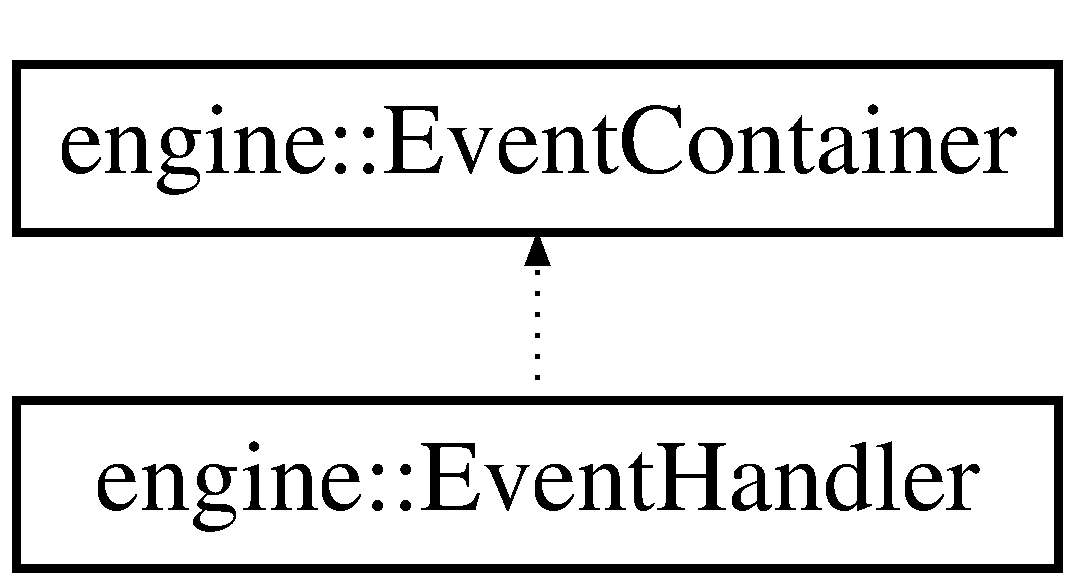
\includegraphics[height=2.000000cm]{a00032}
\end{center}
\end{figure}
\subsubsection*{Public Member Functions}
\begin{DoxyCompactItemize}
\item 
{\bfseries Event\+Container} (const \hyperlink{a00032}{Event\+Container} \&o)\hypertarget{a00032_a589de04f0326a9ea60f46739d11f8bc8}{}\label{a00032_a589de04f0326a9ea60f46739d11f8bc8}

\item 
{\bfseries Event\+Container} (\hyperlink{a00032}{Event\+Container} \&\&o)\hypertarget{a00032_a77b98dd1fd0f7c5ba1e9270964a7e03f}{}\label{a00032_a77b98dd1fd0f7c5ba1e9270964a7e03f}

\item 
\hyperlink{a00032}{Event\+Container} \& {\bfseries operator=} (const \hyperlink{a00032}{Event\+Container} \&o)\hypertarget{a00032_a8fb47de839824ac5cce9b2bbec6a9118}{}\label{a00032_a8fb47de839824ac5cce9b2bbec6a9118}

\item 
\hyperlink{a00032}{Event\+Container} \& {\bfseries operator=} (\hyperlink{a00032}{Event\+Container} \&\&o)\hypertarget{a00032_ad8a227c52cbd142b24adedee6ad2c7c9}{}\label{a00032_ad8a227c52cbd142b24adedee6ad2c7c9}

\end{DoxyCompactItemize}
\subsubsection*{Protected Member Functions}
\begin{DoxyCompactItemize}
\item 
void {\bfseries store\+Event} (std\+::function$<$ void()$>$ \&\&event)\hypertarget{a00032_a58488602891a7963895ba6f5b50b49ef}{}\label{a00032_a58488602891a7963895ba6f5b50b49ef}

\item 
std\+::vector$<$ std\+::function$<$ void()$>$ $>$ {\bfseries clear\+Events} ()\hypertarget{a00032_ac2d38cbe364ea23cb5919d76ad995407}{}\label{a00032_ac2d38cbe364ea23cb5919d76ad995407}

\item 
bool {\bfseries has\+Stored\+Events} () const \hypertarget{a00032_ad8c3610cafce6f79319b7dd4787b47d6}{}\label{a00032_ad8c3610cafce6f79319b7dd4787b47d6}

\end{DoxyCompactItemize}


\subsubsection{Detailed Description}


Definition at line 6 of file Event\+Container.\+h.



The documentation for this class was generated from the following file\+:\begin{DoxyCompactItemize}
\item 
E\+:/\+Programing/\+Projects/\+Engine\+Workspace/\+Common\+Libs/engine/include/engine/events/Event\+Container.\+h\end{DoxyCompactItemize}

\hypertarget{a00033}{}\subsection{engine\+:\+:Event\+Handler Class Reference}
\label{a00033}\index{engine\+::\+Event\+Handler@{engine\+::\+Event\+Handler}}
Inheritance diagram for engine\+:\+:Event\+Handler\+:\begin{figure}[H]
\begin{center}
\leavevmode
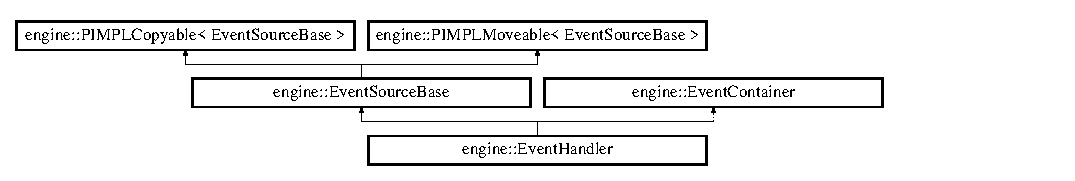
\includegraphics[height=1.985816cm]{a00033}
\end{center}
\end{figure}
\subsubsection*{Public Member Functions}
\begin{DoxyCompactItemize}
\item 
void {\bfseries set\+Events\+Enabled} (bool v)\hypertarget{a00036_ae529242181c16462bef9bd6b8fb56b93}{}\label{a00036_ae529242181c16462bef9bd6b8fb56b93}

\item 
bool {\bfseries is\+Events\+Enabled} () const \hypertarget{a00036_a659325f18d666f132f380e4319499572}{}\label{a00036_a659325f18d666f132f380e4319499572}

\item 
const std\+::string \& {\bfseries get\+Event\+Source\+Id} () const \hypertarget{a00036_ad41deeb2b9de38797b10777e5d1ecf13}{}\label{a00036_ad41deeb2b9de38797b10777e5d1ecf13}

\item 
\hyperlink{a00036}{Event\+Source\+Base} \& {\bfseries P\+I\+M\+P\+L\+Copyable\+::operator=} (const \hyperlink{a00060}{P\+I\+M\+P\+L\+Copyable} \&o)\hypertarget{a00060_a26fdb9b3d449d04dc653c7ae942f452b}{}\label{a00060_a26fdb9b3d449d04dc653c7ae942f452b}

\item 
\hyperlink{a00036}{Event\+Source\+Base} \& {\bfseries P\+I\+M\+P\+L\+Moveable\+::operator=} (\hyperlink{a00061}{P\+I\+M\+P\+L\+Moveable} \&\&o)\hypertarget{a00061_ac67025e8a25edffe99fa9bf67ed8ca19}{}\label{a00061_ac67025e8a25edffe99fa9bf67ed8ca19}

\end{DoxyCompactItemize}
\subsubsection*{Protected Member Functions}
\begin{DoxyCompactItemize}
\item 
{\bfseries Event\+Handler} (const std\+::string \&event\+Source\+Id)\hypertarget{a00033_a6dc8ff476d89c85b4fca87f50707aa94}{}\label{a00033_a6dc8ff476d89c85b4fca87f50707aa94}

\end{DoxyCompactItemize}
\subsubsection*{Private Member Functions}
\begin{DoxyCompactItemize}
\item 
void {\bfseries store\+Event} (std\+::function$<$ void()$>$ \&\&event)\hypertarget{a00032_a58488602891a7963895ba6f5b50b49ef}{}\label{a00032_a58488602891a7963895ba6f5b50b49ef}

\item 
std\+::vector$<$ std\+::function$<$ void()$>$ $>$ {\bfseries clear\+Events} ()\hypertarget{a00032_ac2d38cbe364ea23cb5919d76ad995407}{}\label{a00032_ac2d38cbe364ea23cb5919d76ad995407}

\item 
bool {\bfseries has\+Stored\+Events} () const \hypertarget{a00032_ad8c3610cafce6f79319b7dd4787b47d6}{}\label{a00032_ad8c3610cafce6f79319b7dd4787b47d6}

\end{DoxyCompactItemize}


\subsubsection{Detailed Description}


Definition at line 8 of file Event\+Handler.\+h.



The documentation for this class was generated from the following file\+:\begin{DoxyCompactItemize}
\item 
E\+:/\+Programing/\+Projects/\+Engine\+Workspace/\+Common\+Libs/engine/include/engine/events/Event\+Handler.\+h\end{DoxyCompactItemize}

\hypertarget{a00034}{}\subsection{engine\+:\+:Event\+Manager Class Reference}
\label{a00034}\index{engine\+::\+Event\+Manager@{engine\+::\+Event\+Manager}}
Inheritance diagram for engine\+:\+:Event\+Manager\+:\begin{figure}[H]
\begin{center}
\leavevmode
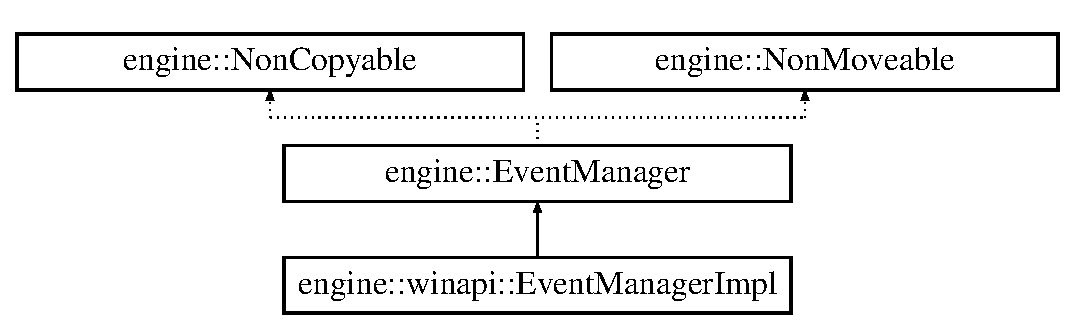
\includegraphics[height=3.000000cm]{a00034}
\end{center}
\end{figure}
\subsubsection*{Public Member Functions}
\begin{DoxyCompactItemize}
\item 
void {\bfseries update} ()\hypertarget{a00034_a5e321019b94d4be4e294951dc15d9bc8}{}\label{a00034_a5e321019b94d4be4e294951dc15d9bc8}

\item 
void {\bfseries add\+Event\+Source} (std\+::unique\+\_\+ptr$<$ \hyperlink{a00036}{Event\+Source\+Base} $>$ \&\&event\+Source)\hypertarget{a00034_ad8ae4d432415974ed273712d621b4b80}{}\label{a00034_ad8ae4d432415974ed273712d621b4b80}

\item 
void {\bfseries register\+Event\+Source} (\hyperlink{a00036}{Event\+Source\+Base} $\ast$)\hypertarget{a00034_a256dc81b8f38d55108fd146075975e76}{}\label{a00034_a256dc81b8f38d55108fd146075975e76}

\item 
void {\bfseries remove\+Event\+Source} (const \hyperlink{a00036}{Event\+Source\+Base} $\ast$)\hypertarget{a00034_ada92665ef93dca332fb60aad4397e741}{}\label{a00034_ada92665ef93dca332fb60aad4397e741}

\item 
std\+::vector$<$ \hyperlink{a00036}{Event\+Source\+Base} $\ast$ $>$ {\bfseries find\+Event\+Source} (const std\+::string \&key) const \hypertarget{a00034_a1973627817da759061278d41dfdf3596}{}\label{a00034_a1973627817da759061278d41dfdf3596}

\item 
{\footnotesize template$<$class T\+\_\+\+Event\+Source $>$ }\\std\+::vector$<$ T\+\_\+\+Event\+Source $\ast$ $>$ {\bfseries find\+Event\+Source} () const \hypertarget{a00034_a8a6707354f1d2dcce3c3c3e0d901c29e}{}\label{a00034_a8a6707354f1d2dcce3c3c3e0d901c29e}

\item 
\hyperlink{a00051}{I\+Signal\+Manager} $\ast$ {\bfseries get\+Events\+Signal\+Manager} () const \hypertarget{a00034_ada7ff964f3ee3c20a34324adc606872b}{}\label{a00034_ada7ff964f3ee3c20a34324adc606872b}

\end{DoxyCompactItemize}
\subsubsection*{Protected Member Functions}
\begin{DoxyCompactItemize}
\item 
std\+::vector$<$ \hyperlink{a00036}{Event\+Source\+Base} $\ast$ $>$ {\bfseries collect\+Event\+Sources} () const \hypertarget{a00034_a06d769343d241b827056389203e1dcb7}{}\label{a00034_a06d769343d241b827056389203e1dcb7}

\end{DoxyCompactItemize}


\subsubsection{Detailed Description}


Definition at line 11 of file Event\+Manager.\+h.



The documentation for this class was generated from the following file\+:\begin{DoxyCompactItemize}
\item 
E\+:/\+Programing/\+Projects/\+Engine\+Workspace/\+Common\+Libs/engine/include/engine/events/Event\+Manager.\+h\end{DoxyCompactItemize}

\hypertarget{a00035}{}\subsection{engine\+:\+:winapi\+:\+:Event\+Manager\+Impl Class Reference}
\label{a00035}\index{engine\+::winapi\+::\+Event\+Manager\+Impl@{engine\+::winapi\+::\+Event\+Manager\+Impl}}
Inheritance diagram for engine\+:\+:winapi\+:\+:Event\+Manager\+Impl\+:\begin{figure}[H]
\begin{center}
\leavevmode
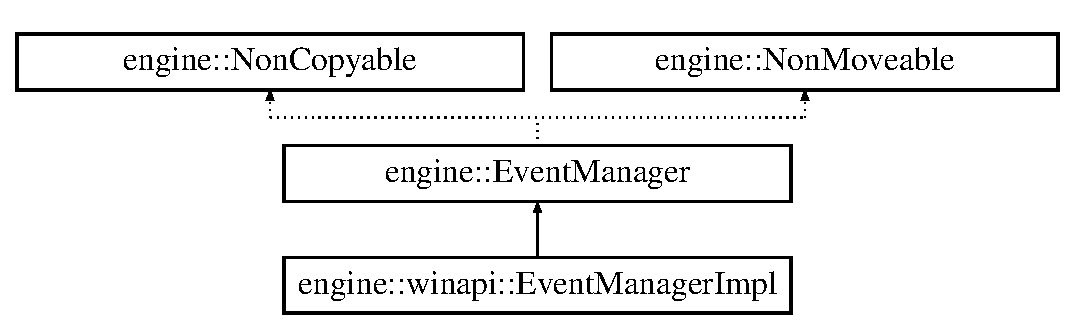
\includegraphics[height=3.000000cm]{a00035}
\end{center}
\end{figure}
\subsubsection*{Public Member Functions}
\begin{DoxyCompactItemize}
\item 
bool {\bfseries handle\+Event} (H\+W\+ND h\+Wnd, U\+I\+NT message, W\+P\+A\+R\+AM w\+Param, L\+P\+A\+R\+AM l\+Param)\hypertarget{a00035_ab3fc7d9983060d9f5cb078f650b00944}{}\label{a00035_ab3fc7d9983060d9f5cb078f650b00944}

\item 
void {\bfseries update} ()\hypertarget{a00034_a5e321019b94d4be4e294951dc15d9bc8}{}\label{a00034_a5e321019b94d4be4e294951dc15d9bc8}

\item 
void {\bfseries add\+Event\+Source} (std\+::unique\+\_\+ptr$<$ \hyperlink{a00036}{Event\+Source\+Base} $>$ \&\&event\+Source)\hypertarget{a00034_ad8ae4d432415974ed273712d621b4b80}{}\label{a00034_ad8ae4d432415974ed273712d621b4b80}

\item 
void {\bfseries register\+Event\+Source} (\hyperlink{a00036}{Event\+Source\+Base} $\ast$)\hypertarget{a00034_a256dc81b8f38d55108fd146075975e76}{}\label{a00034_a256dc81b8f38d55108fd146075975e76}

\item 
void {\bfseries remove\+Event\+Source} (const \hyperlink{a00036}{Event\+Source\+Base} $\ast$)\hypertarget{a00034_ada92665ef93dca332fb60aad4397e741}{}\label{a00034_ada92665ef93dca332fb60aad4397e741}

\item 
std\+::vector$<$ \hyperlink{a00036}{Event\+Source\+Base} $\ast$ $>$ {\bfseries find\+Event\+Source} (const std\+::string \&key) const \hypertarget{a00034_a1973627817da759061278d41dfdf3596}{}\label{a00034_a1973627817da759061278d41dfdf3596}

\item 
{\footnotesize template$<$class T\+\_\+\+Event\+Source $>$ }\\std\+::vector$<$ T\+\_\+\+Event\+Source $\ast$ $>$ {\bfseries find\+Event\+Source} () const \hypertarget{a00034_a8a6707354f1d2dcce3c3c3e0d901c29e}{}\label{a00034_a8a6707354f1d2dcce3c3c3e0d901c29e}

\item 
\hyperlink{a00051}{I\+Signal\+Manager} $\ast$ {\bfseries get\+Events\+Signal\+Manager} () const \hypertarget{a00034_ada7ff964f3ee3c20a34324adc606872b}{}\label{a00034_ada7ff964f3ee3c20a34324adc606872b}

\end{DoxyCompactItemize}
\subsubsection*{Protected Member Functions}
\begin{DoxyCompactItemize}
\item 
std\+::vector$<$ \hyperlink{a00036}{Event\+Source\+Base} $\ast$ $>$ {\bfseries collect\+Event\+Sources} () const \hypertarget{a00034_a06d769343d241b827056389203e1dcb7}{}\label{a00034_a06d769343d241b827056389203e1dcb7}

\end{DoxyCompactItemize}


\subsubsection{Detailed Description}


Definition at line 10 of file Event\+Manager\+Imp.\+h.



The documentation for this class was generated from the following file\+:\begin{DoxyCompactItemize}
\item 
E\+:/\+Programing/\+Projects/\+Engine\+Workspace/\+Common\+Libs/engine/include/engine/events/winapi/Event\+Manager\+Imp.\+h\end{DoxyCompactItemize}

\hypertarget{a00036}{}\subsection{engine\+:\+:Event\+Source\+Base Class Reference}
\label{a00036}\index{engine\+::\+Event\+Source\+Base@{engine\+::\+Event\+Source\+Base}}
Inheritance diagram for engine\+:\+:Event\+Source\+Base\+:\begin{figure}[H]
\begin{center}
\leavevmode
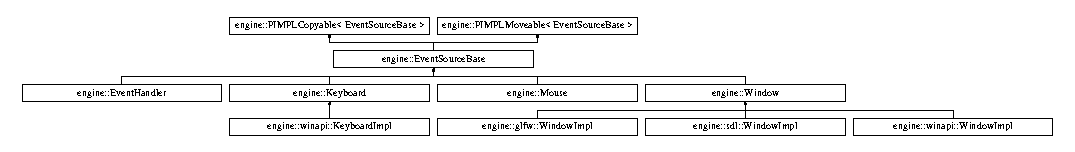
\includegraphics[height=1.588652cm]{a00036}
\end{center}
\end{figure}
\subsubsection*{Public Member Functions}
\begin{DoxyCompactItemize}
\item 
void {\bfseries set\+Events\+Enabled} (bool v)\hypertarget{a00036_ae529242181c16462bef9bd6b8fb56b93}{}\label{a00036_ae529242181c16462bef9bd6b8fb56b93}

\item 
bool {\bfseries is\+Events\+Enabled} () const \hypertarget{a00036_a659325f18d666f132f380e4319499572}{}\label{a00036_a659325f18d666f132f380e4319499572}

\item 
const std\+::string \& {\bfseries get\+Event\+Source\+Id} () const \hypertarget{a00036_ad41deeb2b9de38797b10777e5d1ecf13}{}\label{a00036_ad41deeb2b9de38797b10777e5d1ecf13}

\item 
\hyperlink{a00036}{Event\+Source\+Base} \& {\bfseries P\+I\+M\+P\+L\+Copyable\+::operator=} (const \hyperlink{a00060}{P\+I\+M\+P\+L\+Copyable} \&o)\hypertarget{a00060_a26fdb9b3d449d04dc653c7ae942f452b}{}\label{a00060_a26fdb9b3d449d04dc653c7ae942f452b}

\item 
\hyperlink{a00036}{Event\+Source\+Base} \& {\bfseries P\+I\+M\+P\+L\+Moveable\+::operator=} (\hyperlink{a00061}{P\+I\+M\+P\+L\+Moveable} \&\&o)\hypertarget{a00061_ac67025e8a25edffe99fa9bf67ed8ca19}{}\label{a00061_ac67025e8a25edffe99fa9bf67ed8ca19}

\end{DoxyCompactItemize}
\subsubsection*{Protected Member Functions}
\begin{DoxyCompactItemize}
\item 
{\bfseries Event\+Source\+Base} (const std\+::string \&event\+Source\+Id)\hypertarget{a00036_aaf869f7f30d31a3eb2713937e8a8f902}{}\label{a00036_aaf869f7f30d31a3eb2713937e8a8f902}

\end{DoxyCompactItemize}


\subsubsection{Detailed Description}


Definition at line 9 of file Event\+Source\+Base.\+h.



The documentation for this class was generated from the following file\+:\begin{DoxyCompactItemize}
\item 
E\+:/\+Programing/\+Projects/\+Engine\+Workspace/\+Common\+Libs/engine/include/engine/events/Event\+Source\+Base.\+h\end{DoxyCompactItemize}

\hypertarget{a00037}{}\subsection{engine\+:\+:Expired\+Error Struct Reference}
\label{a00037}\index{engine\+::\+Expired\+Error@{engine\+::\+Expired\+Error}}
Inheritance diagram for engine\+:\+:Expired\+Error\+:\begin{figure}[H]
\begin{center}
\leavevmode
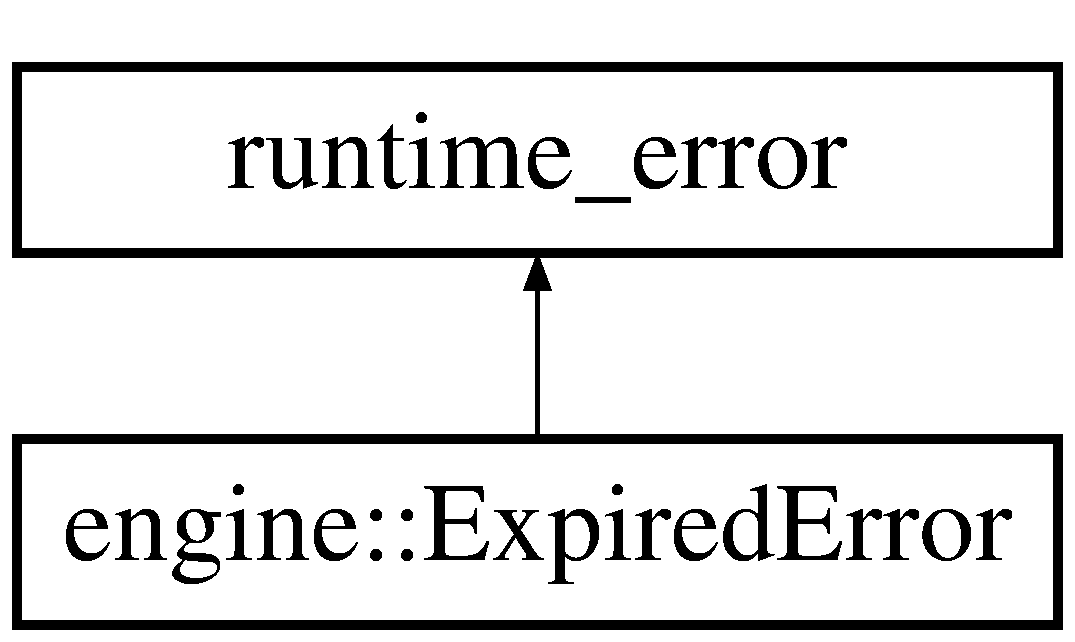
\includegraphics[height=2.000000cm]{a00037}
\end{center}
\end{figure}
\subsubsection*{Public Member Functions}
\begin{DoxyCompactItemize}
\item 
{\bfseries Expired\+Error} (const std\+::string \&error)\hypertarget{a00037_ab18d5a73cd058d28d2ea936947fe0376}{}\label{a00037_ab18d5a73cd058d28d2ea936947fe0376}

\item 
{\bfseries Expired\+Error} (const char $\ast$error)\hypertarget{a00037_a653e8cc0b1b14f5629c9e1592fd487f1}{}\label{a00037_a653e8cc0b1b14f5629c9e1592fd487f1}

\end{DoxyCompactItemize}


\subsubsection{Detailed Description}


Definition at line 7 of file Runtime\+Errors.\+h.



The documentation for this struct was generated from the following file\+:\begin{DoxyCompactItemize}
\item 
E\+:/\+Programing/\+Projects/\+Engine\+Workspace/\+Common\+Libs/engine/include/engine/exceptions/Runtime\+Errors.\+h\end{DoxyCompactItemize}

\hypertarget{a00038}{}\subsection{engine\+:\+:Game Class Reference}
\label{a00038}\index{engine\+::\+Game@{engine\+::\+Game}}


{\ttfamily \#include $<$E\+:/\+Programing/\+Projects/\+Engine\+Workspace/\+Common\+Libs/engine/include/engine/app/\+Game.\+h$>$}

Inheritance diagram for engine\+:\+:Game\+:\begin{figure}[H]
\begin{center}
\leavevmode
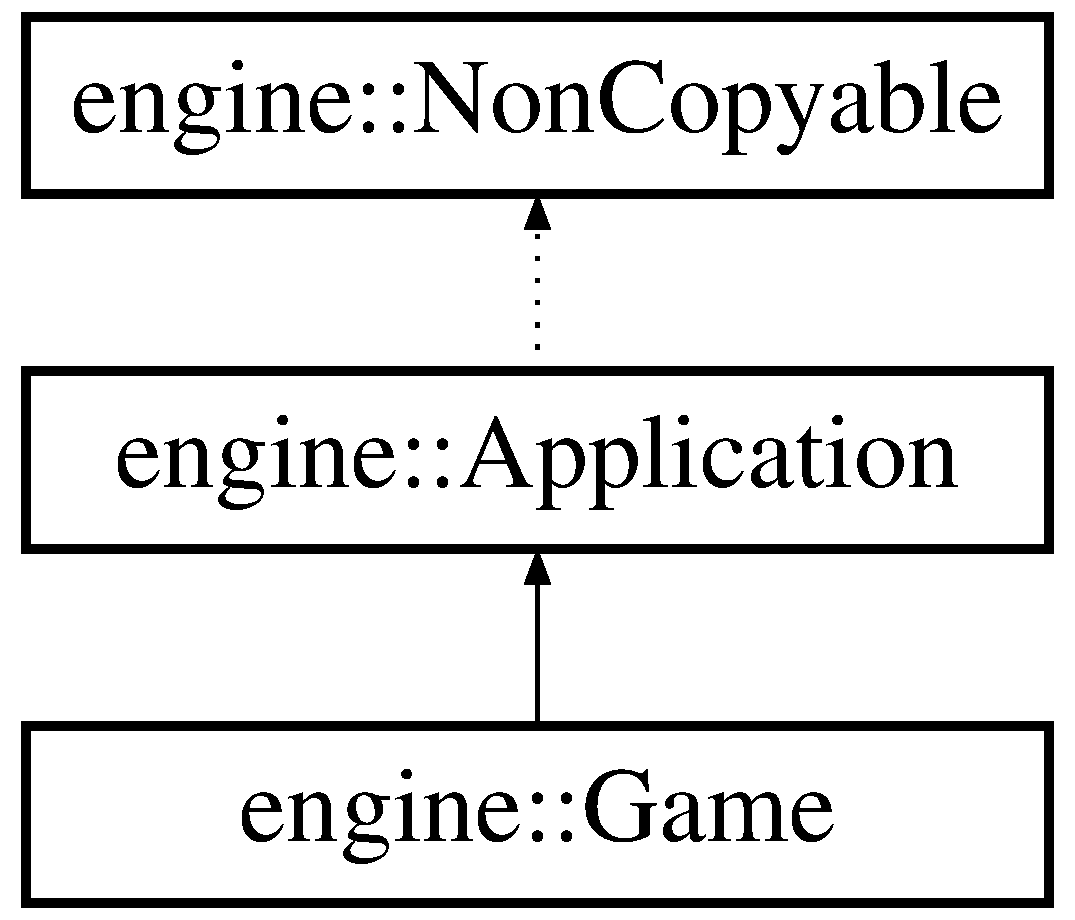
\includegraphics[height=3.000000cm]{a00038}
\end{center}
\end{figure}
\subsubsection*{Public Member Functions}
\begin{DoxyCompactItemize}
\item 
\hyperlink{a00038_a9b20c295fd6af60e00709da9ff9cde89}{Game} (std\+::unique\+\_\+ptr$<$ \hyperlink{a00043}{I\+Application\+Parameter} $>$ arguments, std\+::unique\+\_\+ptr$<$ \hyperlink{a00045}{I\+Main} $>$ main)
\item 
\hyperlink{a00038_a36ee1fe045159234e2916e20f0d94562}{$\sim$\+Game} ()
\item 
void \hyperlink{a00038_a395e9435f60c020fb7687f23e4ebca3a}{set\+Start\+State} (std\+::unique\+\_\+ptr$<$ \hyperlink{a00072}{engine\+::\+State\+Base} $>$ start\+State)
\item 
void {\bfseries run} ()\hypertarget{a00002_a6d9c94380f1451664ff6d09c314671c7}{}\label{a00002_a6d9c94380f1451664ff6d09c314671c7}

\item 
void \hyperlink{a00002_a149822f20163e98d41728f4752d7a7f7}{update} ()
\item 
void \hyperlink{a00002_af3ef70b1c3e25be0dbe68c460ec2db98}{render} ()
\item 
bool \hyperlink{a00002_a86f249cf621c4255df1a60987c588961}{is\+Active} () const 
\item 
void \hyperlink{a00002_aeb61beceae055e7681b6791dd5dddafa}{stop} ()
\item 
void \hyperlink{a00002_a9b8b10fd48e93db0986df610523105dc}{start} ()
\item 
const \hyperlink{a00043}{I\+Application\+Parameter} $\ast$ \hyperlink{a00002_af165b483b86469ff9db2f689f1212f14}{get\+Arguments} () const 
\item 
\hyperlink{a00034}{Event\+Manager} $\ast$ {\bfseries get\+Event\+Manager} () const \hypertarget{a00002_aa895c5c2a56efe782cd9cb038075bb60}{}\label{a00002_aa895c5c2a56efe782cd9cb038075bb60}

\item 
\hyperlink{a00087}{Window\+Manager} $\ast$ {\bfseries get\+Window\+Manager} () const \hypertarget{a00002_aed35eca596bce4c089aa3db72d3dc5b6}{}\label{a00002_aed35eca596bce4c089aa3db72d3dc5b6}

\end{DoxyCompactItemize}


\subsubsection{Detailed Description}
A game is a special application which has a state machine inside on it. 

Definition at line 14 of file Game.\+h.



\subsubsection{Constructor \& Destructor Documentation}
\index{engine\+::\+Game@{engine\+::\+Game}!Game@{Game}}
\index{Game@{Game}!engine\+::\+Game@{engine\+::\+Game}}
\paragraph[{\texorpdfstring{Game(std\+::unique\+\_\+ptr$<$ I\+Application\+Parameter $>$ arguments, std\+::unique\+\_\+ptr$<$ I\+Main $>$ main)}{Game(std::unique_ptr< IApplicationParameter > arguments, std::unique_ptr< IMain > main)}}]{\setlength{\rightskip}{0pt plus 5cm}engine\+::\+Game\+::\+Game (
\begin{DoxyParamCaption}
\item[{std\+::unique\+\_\+ptr$<$ {\bf I\+Application\+Parameter} $>$}]{arguments, }
\item[{std\+::unique\+\_\+ptr$<$ {\bf I\+Main} $>$}]{main}
\end{DoxyParamCaption}
)}\hypertarget{a00038_a9b20c295fd6af60e00709da9ff9cde89}{}\label{a00038_a9b20c295fd6af60e00709da9ff9cde89}
\begin{DoxySeeAlso}{See also}
\hyperlink{a00002_a8ba1a5c0ffacfa8c22797d62722f1359}{Application\+::\+Application} 
\end{DoxySeeAlso}
\index{engine\+::\+Game@{engine\+::\+Game}!````~Game@{$\sim$\+Game}}
\index{````~Game@{$\sim$\+Game}!engine\+::\+Game@{engine\+::\+Game}}
\paragraph[{\texorpdfstring{$\sim$\+Game()}{~Game()}}]{\setlength{\rightskip}{0pt plus 5cm}engine\+::\+Game\+::$\sim$\+Game (
\begin{DoxyParamCaption}
{}
\end{DoxyParamCaption}
)}\hypertarget{a00038_a36ee1fe045159234e2916e20f0d94562}{}\label{a00038_a36ee1fe045159234e2916e20f0d94562}
Destructor for P\+I\+M\+PL 

\subsubsection{Member Function Documentation}
\index{engine\+::\+Game@{engine\+::\+Game}!get\+Arguments@{get\+Arguments}}
\index{get\+Arguments@{get\+Arguments}!engine\+::\+Game@{engine\+::\+Game}}
\paragraph[{\texorpdfstring{get\+Arguments() const }{getArguments() const }}]{\setlength{\rightskip}{0pt plus 5cm}const {\bf I\+Application\+Parameter}$\ast$ engine\+::\+Application\+::get\+Arguments (
\begin{DoxyParamCaption}
{}
\end{DoxyParamCaption}
) const\hspace{0.3cm}{\ttfamily [inherited]}}\hypertarget{a00002_af165b483b86469ff9db2f689f1212f14}{}\label{a00002_af165b483b86469ff9db2f689f1212f14}
\begin{DoxyReturn}{Returns}
Returns the initial arguments of the application 
\end{DoxyReturn}
\index{engine\+::\+Game@{engine\+::\+Game}!is\+Active@{is\+Active}}
\index{is\+Active@{is\+Active}!engine\+::\+Game@{engine\+::\+Game}}
\paragraph[{\texorpdfstring{is\+Active() const }{isActive() const }}]{\setlength{\rightskip}{0pt plus 5cm}bool engine\+::\+Application\+::is\+Active (
\begin{DoxyParamCaption}
{}
\end{DoxyParamCaption}
) const\hspace{0.3cm}{\ttfamily [inherited]}}\hypertarget{a00002_a86f249cf621c4255df1a60987c588961}{}\label{a00002_a86f249cf621c4255df1a60987c588961}
\begin{DoxyReturn}{Returns}
Returns true till the application is not terminated. 
\end{DoxyReturn}
\index{engine\+::\+Game@{engine\+::\+Game}!render@{render}}
\index{render@{render}!engine\+::\+Game@{engine\+::\+Game}}
\paragraph[{\texorpdfstring{render()}{render()}}]{\setlength{\rightskip}{0pt plus 5cm}void engine\+::\+Application\+::render (
\begin{DoxyParamCaption}
{}
\end{DoxyParamCaption}
)\hspace{0.3cm}{\ttfamily [inherited]}}\hypertarget{a00002_af3ef70b1c3e25be0dbe68c460ec2db98}{}\label{a00002_af3ef70b1c3e25be0dbe68c460ec2db98}
Render is called in each frame. Here will be rendered the application \index{engine\+::\+Game@{engine\+::\+Game}!set\+Start\+State@{set\+Start\+State}}
\index{set\+Start\+State@{set\+Start\+State}!engine\+::\+Game@{engine\+::\+Game}}
\paragraph[{\texorpdfstring{set\+Start\+State(std\+::unique\+\_\+ptr$<$ engine\+::\+State\+Base $>$ start\+State)}{setStartState(std::unique_ptr< engine::StateBase > startState)}}]{\setlength{\rightskip}{0pt plus 5cm}void engine\+::\+Game\+::set\+Start\+State (
\begin{DoxyParamCaption}
\item[{std\+::unique\+\_\+ptr$<$ {\bf engine\+::\+State\+Base} $>$}]{start\+State}
\end{DoxyParamCaption}
)}\hypertarget{a00038_a395e9435f60c020fb7687f23e4ebca3a}{}\label{a00038_a395e9435f60c020fb7687f23e4ebca3a}
Set the start state 
\begin{DoxyParams}{Parameters}
{\em start\+State} & State which will be active when the game is started. \\
\hline
\end{DoxyParams}
\index{engine\+::\+Game@{engine\+::\+Game}!start@{start}}
\index{start@{start}!engine\+::\+Game@{engine\+::\+Game}}
\paragraph[{\texorpdfstring{start()}{start()}}]{\setlength{\rightskip}{0pt plus 5cm}void engine\+::\+Application\+::start (
\begin{DoxyParamCaption}
{}
\end{DoxyParamCaption}
)\hspace{0.3cm}{\ttfamily [inherited]}}\hypertarget{a00002_a9b8b10fd48e93db0986df610523105dc}{}\label{a00002_a9b8b10fd48e93db0986df610523105dc}
Terminate the application \index{engine\+::\+Game@{engine\+::\+Game}!stop@{stop}}
\index{stop@{stop}!engine\+::\+Game@{engine\+::\+Game}}
\paragraph[{\texorpdfstring{stop()}{stop()}}]{\setlength{\rightskip}{0pt plus 5cm}void engine\+::\+Application\+::stop (
\begin{DoxyParamCaption}
{}
\end{DoxyParamCaption}
)\hspace{0.3cm}{\ttfamily [inherited]}}\hypertarget{a00002_aeb61beceae055e7681b6791dd5dddafa}{}\label{a00002_aeb61beceae055e7681b6791dd5dddafa}
Starts the application. \index{engine\+::\+Game@{engine\+::\+Game}!update@{update}}
\index{update@{update}!engine\+::\+Game@{engine\+::\+Game}}
\paragraph[{\texorpdfstring{update()}{update()}}]{\setlength{\rightskip}{0pt plus 5cm}void engine\+::\+Application\+::update (
\begin{DoxyParamCaption}
{}
\end{DoxyParamCaption}
)\hspace{0.3cm}{\ttfamily [inherited]}}\hypertarget{a00002_a149822f20163e98d41728f4752d7a7f7}{}\label{a00002_a149822f20163e98d41728f4752d7a7f7}
Update is called once per each frame 

The documentation for this class was generated from the following file\+:\begin{DoxyCompactItemize}
\item 
E\+:/\+Programing/\+Projects/\+Engine\+Workspace/\+Common\+Libs/engine/include/engine/app/Game.\+h\end{DoxyCompactItemize}

\hypertarget{a00039}{}\subsection{engine\+:\+:test\+:\+:Game\+Assert\+Exception Class Reference}
\label{a00039}\index{engine\+::test\+::\+Game\+Assert\+Exception@{engine\+::test\+::\+Game\+Assert\+Exception}}
\subsubsection*{Public Types}
\begin{DoxyCompactItemize}
\item 
enum {\bfseries Type} \{ {\bfseries Hard}, 
{\bfseries Normal}
 \}\hypertarget{a00039_adb341c9f0035716e556fbbb858815562}{}\label{a00039_adb341c9f0035716e556fbbb858815562}

\end{DoxyCompactItemize}
\subsubsection*{Public Member Functions}
\begin{DoxyCompactItemize}
\item 
{\bfseries Game\+Assert\+Exception} (Type type, const std\+::string \&message, const std\+::string \&file, const uint32\+\_\+t line)\hypertarget{a00039_a67de0ef29f112f3ad99e5cf1f59639c5}{}\label{a00039_a67de0ef29f112f3ad99e5cf1f59639c5}

\item 
{\bfseries Game\+Assert\+Exception} (const \hyperlink{a00039}{Game\+Assert\+Exception} \&o)\hypertarget{a00039_a5d45ad5614324c6ff6288095c49bef86}{}\label{a00039_a5d45ad5614324c6ff6288095c49bef86}

\item 
{\bfseries Game\+Assert\+Exception} (\hyperlink{a00039}{Game\+Assert\+Exception} \&\&o)\hypertarget{a00039_a0adcc77c72447b144af620a848786c08}{}\label{a00039_a0adcc77c72447b144af620a848786c08}

\item 
Type {\bfseries get\+Type} () const \hypertarget{a00039_af7c02390f1a36a2ef5b503daaa71b26c}{}\label{a00039_af7c02390f1a36a2ef5b503daaa71b26c}

\item 
const std\+::string \& {\bfseries get\+Message} () const \hypertarget{a00039_a9c691825de7209dda1afa81ab96c24f9}{}\label{a00039_a9c691825de7209dda1afa81ab96c24f9}

\item 
const std\+::string \& {\bfseries get\+File} () const \hypertarget{a00039_a42c238d2506f39c71b132fd5434afcfe}{}\label{a00039_a42c238d2506f39c71b132fd5434afcfe}

\item 
uint32\+\_\+t {\bfseries get\+Line} () const \hypertarget{a00039_a2a42499a575063750e93d8f477b00682}{}\label{a00039_a2a42499a575063750e93d8f477b00682}

\end{DoxyCompactItemize}


\subsubsection{Detailed Description}


Definition at line 7 of file Game\+Assert\+Exception.\+h.



The documentation for this class was generated from the following file\+:\begin{DoxyCompactItemize}
\item 
E\+:/\+Programing/\+Projects/\+Engine\+Workspace/\+Common\+Libs/engine/include/engine/test/Game\+Assert\+Exception.\+h\end{DoxyCompactItemize}

\hypertarget{a00040}{}\subsection{engine\+:\+:Gen\+Sequence$<$ N, Is $>$ Struct Template Reference}
\label{a00040}\index{engine\+::\+Gen\+Sequence$<$ N, Is $>$@{engine\+::\+Gen\+Sequence$<$ N, Is $>$}}


{\ttfamily \#include $<$E\+:/\+Programing/\+Projects/\+Engine\+Workspace/\+Common\+Libs/engine/include/engine/utils/\+Gen\+Sequence.\+h$>$}



\subsubsection{Detailed Description}
\subsubsection*{template$<$int N, int... Is$>$\\*
struct engine\+::\+Gen\+Sequence$<$ N, Is $>$}

Generate compile time sequence, like Index$<$5, 4, 3, 2, 1$>$. It is really usefull for generate placeholders in compile time 

Definition at line 14 of file Gen\+Sequence.\+h.



The documentation for this struct was generated from the following file\+:\begin{DoxyCompactItemize}
\item 
E\+:/\+Programing/\+Projects/\+Engine\+Workspace/\+Common\+Libs/engine/include/engine/utils/Gen\+Sequence.\+h\end{DoxyCompactItemize}

\hypertarget{a00041}{}\subsection{engine\+:\+:Gen\+Sequence$<$ 0, Is... $>$ Struct Template Reference}
\label{a00041}\index{engine\+::\+Gen\+Sequence$<$ 0, Is... $>$@{engine\+::\+Gen\+Sequence$<$ 0, Is... $>$}}


{\ttfamily \#include $<$E\+:/\+Programing/\+Projects/\+Engine\+Workspace/\+Common\+Libs/engine/include/engine/utils/\+Gen\+Sequence.\+h$>$}

Inheritance diagram for engine\+:\+:Gen\+Sequence$<$ 0, Is... $>$\+:\begin{figure}[H]
\begin{center}
\leavevmode
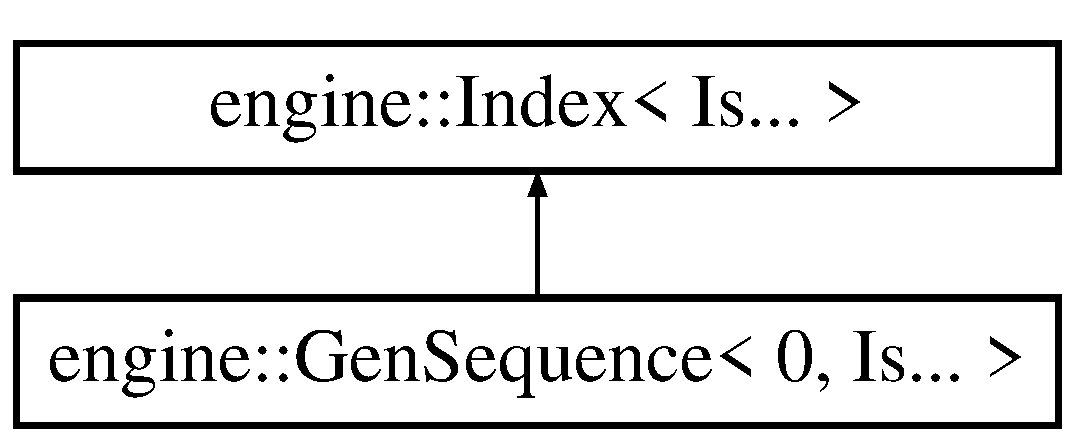
\includegraphics[height=2.000000cm]{a00041}
\end{center}
\end{figure}


\subsubsection{Detailed Description}
\subsubsection*{template$<$int... Is$>$\\*
struct engine\+::\+Gen\+Sequence$<$ 0, Is... $>$}

Final element 

Definition at line 18 of file Gen\+Sequence.\+h.



The documentation for this struct was generated from the following file\+:\begin{DoxyCompactItemize}
\item 
E\+:/\+Programing/\+Projects/\+Engine\+Workspace/\+Common\+Libs/engine/include/engine/utils/Gen\+Sequence.\+h\end{DoxyCompactItemize}

\hypertarget{a00042}{}\subsection{engine\+:\+:glfw\+:\+:Buffer\+Desc\+Utils\+:\+:Glfw\+Desc Struct Reference}
\label{a00042}\index{engine\+::glfw\+::\+Buffer\+Desc\+Utils\+::\+Glfw\+Desc@{engine\+::glfw\+::\+Buffer\+Desc\+Utils\+::\+Glfw\+Desc}}
\subsubsection*{Public Attributes}
\begin{DoxyCompactItemize}
\item 
int32\+\_\+t {\bfseries red\+Bits} = 0\hypertarget{a00042_a2c5c19f8fdecd7ff6b53ffdcc7ca2a93}{}\label{a00042_a2c5c19f8fdecd7ff6b53ffdcc7ca2a93}

\item 
int32\+\_\+t {\bfseries blue\+Bits} = 0\hypertarget{a00042_ad162b71247141e47b5e42a7def102b26}{}\label{a00042_ad162b71247141e47b5e42a7def102b26}

\item 
int32\+\_\+t {\bfseries green\+Bits} = 0\hypertarget{a00042_a161ee120c160dd36d7a42389101ec6d6}{}\label{a00042_a161ee120c160dd36d7a42389101ec6d6}

\item 
int32\+\_\+t {\bfseries alpha\+Bits} = 0\hypertarget{a00042_a488c03ac5a2cb6e968516e4062ff6c1f}{}\label{a00042_a488c03ac5a2cb6e968516e4062ff6c1f}

\item 
int32\+\_\+t {\bfseries stencil\+Bits} = 0\hypertarget{a00042_a6b3341927ea496b51aeb04c9c99569b2}{}\label{a00042_a6b3341927ea496b51aeb04c9c99569b2}

\item 
int32\+\_\+t {\bfseries depth\+Bits} = 0\hypertarget{a00042_ac27b9115a46506f023f163ec0ac25802}{}\label{a00042_ac27b9115a46506f023f163ec0ac25802}

\item 
bool {\bfseries use\+Srgb} = false\hypertarget{a00042_a7faef9279f4dd062aa5bd55daeae2dbe}{}\label{a00042_a7faef9279f4dd062aa5bd55daeae2dbe}

\end{DoxyCompactItemize}


\subsubsection{Detailed Description}


Definition at line 14 of file Buffer\+Desc\+Utils.\+h.



The documentation for this struct was generated from the following file\+:\begin{DoxyCompactItemize}
\item 
E\+:/\+Programing/\+Projects/\+Engine\+Workspace/\+Common\+Libs/engine/include/engine/video/glfw/Buffer\+Desc\+Utils.\+h\end{DoxyCompactItemize}

\hypertarget{a00043}{}\subsection{engine\+:\+:I\+Application\+Parameter Class Reference}
\label{a00043}\index{engine\+::\+I\+Application\+Parameter@{engine\+::\+I\+Application\+Parameter}}


{\ttfamily \#include $<$E\+:/\+Programing/\+Projects/\+Engine\+Workspace/\+Common\+Libs/engine/include/engine/app/\+I\+Application\+Parameter.\+h$>$}

Inheritance diagram for engine\+:\+:I\+Application\+Parameter\+:\begin{figure}[H]
\begin{center}
\leavevmode
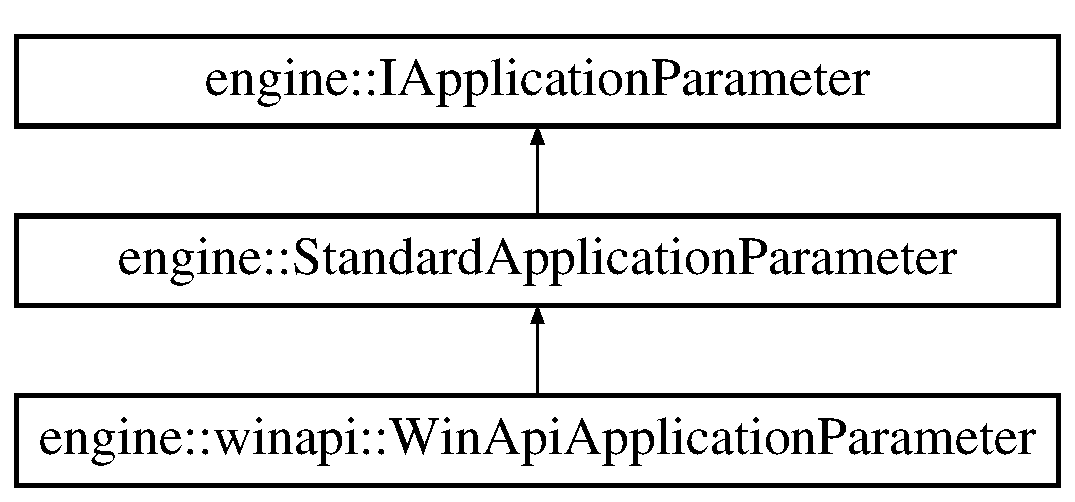
\includegraphics[height=3.000000cm]{a00043}
\end{center}
\end{figure}


\subsubsection{Detailed Description}
Common interface for application parameters 

Definition at line 6 of file I\+Application\+Parameter.\+h.



The documentation for this class was generated from the following file\+:\begin{DoxyCompactItemize}
\item 
E\+:/\+Programing/\+Projects/\+Engine\+Workspace/\+Common\+Libs/engine/include/engine/app/I\+Application\+Parameter.\+h\end{DoxyCompactItemize}

\hypertarget{a00044}{}\subsection{engine\+:\+:Id\+Generator$<$ T\+AG $>$ Class Template Reference}
\label{a00044}\index{engine\+::\+Id\+Generator$<$ T\+A\+G $>$@{engine\+::\+Id\+Generator$<$ T\+A\+G $>$}}


{\ttfamily \#include $<$E\+:/\+Programing/\+Projects/\+Engine\+Workspace/\+Common\+Libs/engine/include/engine/utils/\+Id\+Generator.\+h$>$}

\subsubsection*{Static Public Member Functions}
\begin{DoxyCompactItemize}
\item 
static uint32\+\_\+t \hyperlink{a00044_a211645f2f83332a1fb76671cfffd638c}{generate\+Next\+Id} ()
\end{DoxyCompactItemize}


\subsubsection{Detailed Description}
\subsubsection*{template$<$typename T\+AG$>$\\*
class engine\+::\+Id\+Generator$<$ T\+A\+G $>$}

Helper class for id generation based on tag. Thread safe. 

Definition at line 13 of file Id\+Generator.\+h.



\subsubsection{Member Function Documentation}
\index{engine\+::\+Id\+Generator@{engine\+::\+Id\+Generator}!generate\+Next\+Id@{generate\+Next\+Id}}
\index{generate\+Next\+Id@{generate\+Next\+Id}!engine\+::\+Id\+Generator@{engine\+::\+Id\+Generator}}
\paragraph[{\texorpdfstring{generate\+Next\+Id()}{generateNextId()}}]{\setlength{\rightskip}{0pt plus 5cm}template$<$typename T\+AG $>$ uint32\+\_\+t {\bf engine\+::\+Id\+Generator}$<$ T\+AG $>$\+::generate\+Next\+Id (
\begin{DoxyParamCaption}
{}
\end{DoxyParamCaption}
)\hspace{0.3cm}{\ttfamily [static]}}\hypertarget{a00044_a211645f2f83332a1fb76671cfffd638c}{}\label{a00044_a211645f2f83332a1fb76671cfffd638c}
Generates a next id 

Definition at line 27 of file Id\+Generator.\+h.



The documentation for this class was generated from the following file\+:\begin{DoxyCompactItemize}
\item 
E\+:/\+Programing/\+Projects/\+Engine\+Workspace/\+Common\+Libs/engine/include/engine/utils/Id\+Generator.\+h\end{DoxyCompactItemize}

\hypertarget{a00045}{}\subsection{engine\+:\+:I\+Main Class Reference}
\label{a00045}\index{engine\+::\+I\+Main@{engine\+::\+I\+Main}}


{\ttfamily \#include $<$E\+:/\+Programing/\+Projects/\+Engine\+Workspace/\+Common\+Libs/engine/include/engine/app/\+I\+Main.\+h$>$}

Inheritance diagram for engine\+:\+:I\+Main\+:\begin{figure}[H]
\begin{center}
\leavevmode
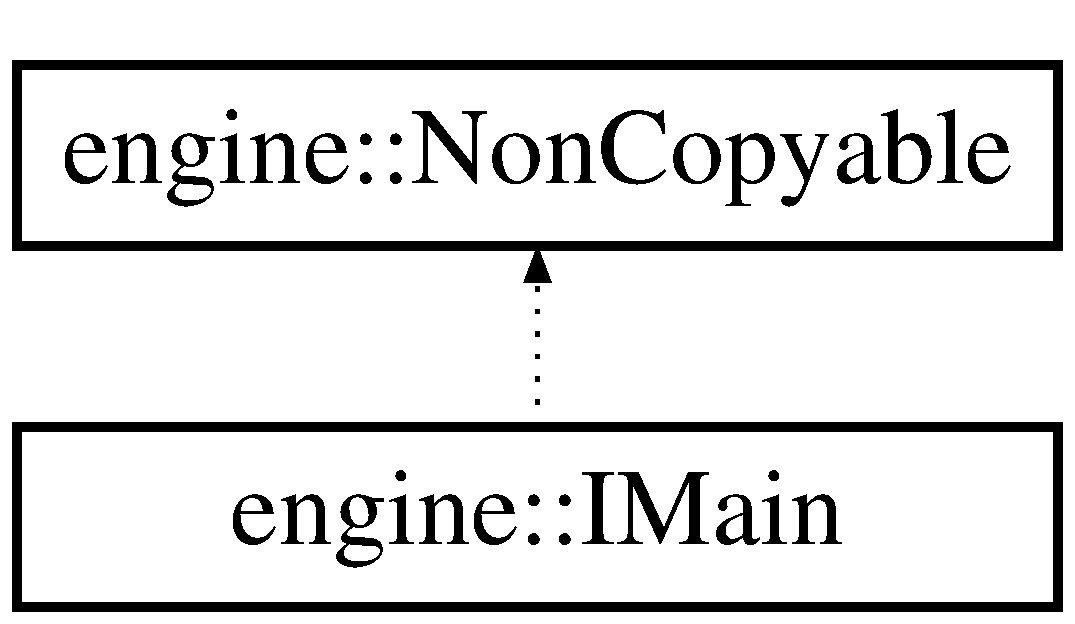
\includegraphics[height=2.000000cm]{a00045}
\end{center}
\end{figure}
\subsubsection*{Public Member Functions}
\begin{DoxyCompactItemize}
\item 
\hyperlink{a00045_a3e512e4387b1517f99466e1eb01e0d78}{$\sim$\+I\+Main} ()
\item 
virtual void \hyperlink{a00045_aaddfdf70642e7bd6df3256e7074fa571}{load} ()=0
\item 
virtual void \hyperlink{a00045_a6ae095ca594d7ad67704efc97bb50adf}{update} ()=0
\item 
virtual void \hyperlink{a00045_abf626b47003850fbfb5fc334409c80ec}{render} ()=0
\end{DoxyCompactItemize}
\subsubsection*{Protected Member Functions}
\begin{DoxyCompactItemize}
\item 
\hyperlink{a00045_a7123c5ea514a788ba01089f3a257b72b}{I\+Main} ()=default
\end{DoxyCompactItemize}


\subsubsection{Detailed Description}
Base class for core logic of an application 

Definition at line 11 of file I\+Main.\+h.



\subsubsection{Constructor \& Destructor Documentation}
\index{engine\+::\+I\+Main@{engine\+::\+I\+Main}!I\+Main@{I\+Main}}
\index{I\+Main@{I\+Main}!engine\+::\+I\+Main@{engine\+::\+I\+Main}}
\paragraph[{\texorpdfstring{I\+Main()=default}{IMain()=default}}]{\setlength{\rightskip}{0pt plus 5cm}engine\+::\+I\+Main\+::\+I\+Main (
\begin{DoxyParamCaption}
{}
\end{DoxyParamCaption}
)\hspace{0.3cm}{\ttfamily [protected]}, {\ttfamily [default]}}\hypertarget{a00045_a7123c5ea514a788ba01089f3a257b72b}{}\label{a00045_a7123c5ea514a788ba01089f3a257b72b}
Simple constructor only for child classes. \index{engine\+::\+I\+Main@{engine\+::\+I\+Main}!````~I\+Main@{$\sim$\+I\+Main}}
\index{````~I\+Main@{$\sim$\+I\+Main}!engine\+::\+I\+Main@{engine\+::\+I\+Main}}
\paragraph[{\texorpdfstring{$\sim$\+I\+Main()}{~IMain()}}]{\setlength{\rightskip}{0pt plus 5cm}engine\+::\+I\+Main\+::$\sim$\+I\+Main (
\begin{DoxyParamCaption}
{}
\end{DoxyParamCaption}
)\hspace{0.3cm}{\ttfamily [inline]}}\hypertarget{a00045_a3e512e4387b1517f99466e1eb01e0d78}{}\label{a00045_a3e512e4387b1517f99466e1eb01e0d78}
Simple destructor 

Definition at line 18 of file I\+Main.\+h.



\subsubsection{Member Function Documentation}
\index{engine\+::\+I\+Main@{engine\+::\+I\+Main}!load@{load}}
\index{load@{load}!engine\+::\+I\+Main@{engine\+::\+I\+Main}}
\paragraph[{\texorpdfstring{load()=0}{load()=0}}]{\setlength{\rightskip}{0pt plus 5cm}virtual void engine\+::\+I\+Main\+::load (
\begin{DoxyParamCaption}
{}
\end{DoxyParamCaption}
)\hspace{0.3cm}{\ttfamily [pure virtual]}}\hypertarget{a00045_aaddfdf70642e7bd6df3256e7074fa571}{}\label{a00045_aaddfdf70642e7bd6df3256e7074fa571}
Called once when the application is started 

Referenced by $\sim$\+I\+Main().

\index{engine\+::\+I\+Main@{engine\+::\+I\+Main}!render@{render}}
\index{render@{render}!engine\+::\+I\+Main@{engine\+::\+I\+Main}}
\paragraph[{\texorpdfstring{render()=0}{render()=0}}]{\setlength{\rightskip}{0pt plus 5cm}virtual void engine\+::\+I\+Main\+::render (
\begin{DoxyParamCaption}
{}
\end{DoxyParamCaption}
)\hspace{0.3cm}{\ttfamily [pure virtual]}}\hypertarget{a00045_abf626b47003850fbfb5fc334409c80ec}{}\label{a00045_abf626b47003850fbfb5fc334409c80ec}
Called once per each frame to render 

Referenced by $\sim$\+I\+Main().

\index{engine\+::\+I\+Main@{engine\+::\+I\+Main}!update@{update}}
\index{update@{update}!engine\+::\+I\+Main@{engine\+::\+I\+Main}}
\paragraph[{\texorpdfstring{update()=0}{update()=0}}]{\setlength{\rightskip}{0pt plus 5cm}virtual void engine\+::\+I\+Main\+::update (
\begin{DoxyParamCaption}
{}
\end{DoxyParamCaption}
)\hspace{0.3cm}{\ttfamily [pure virtual]}}\hypertarget{a00045_a6ae095ca594d7ad67704efc97bb50adf}{}\label{a00045_a6ae095ca594d7ad67704efc97bb50adf}
Called once per each frame to update the main 

Referenced by $\sim$\+I\+Main().



The documentation for this class was generated from the following file\+:\begin{DoxyCompactItemize}
\item 
E\+:/\+Programing/\+Projects/\+Engine\+Workspace/\+Common\+Libs/engine/include/engine/app/I\+Main.\+h\end{DoxyCompactItemize}

\hypertarget{a00046}{}\subsection{engine\+:\+:I\+Module\+Extension Struct Reference}
\label{a00046}\index{engine\+::\+I\+Module\+Extension@{engine\+::\+I\+Module\+Extension}}
Inheritance diagram for engine\+:\+:I\+Module\+Extension\+:\begin{figure}[H]
\begin{center}
\leavevmode
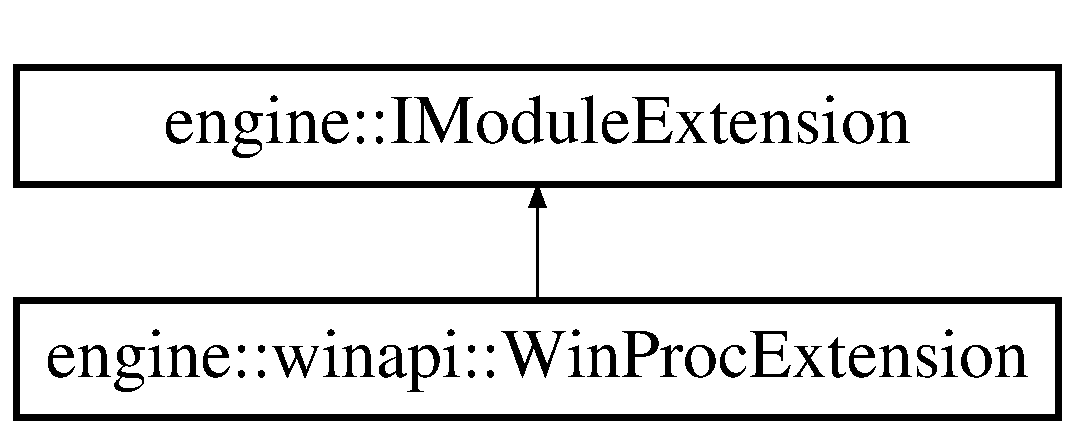
\includegraphics[height=2.000000cm]{a00046}
\end{center}
\end{figure}


\subsubsection{Detailed Description}


Definition at line 5 of file I\+Module\+Extension.\+h.



The documentation for this struct was generated from the following file\+:\begin{DoxyCompactItemize}
\item 
E\+:/\+Programing/\+Projects/\+Engine\+Workspace/\+Common\+Libs/engine/include/engine/I\+Module\+Extension.\+h\end{DoxyCompactItemize}

\hypertarget{a00047}{}\subsection{engine\+:\+:Index$<$ Is $>$ Struct Template Reference}
\label{a00047}\index{engine\+::\+Index$<$ Is $>$@{engine\+::\+Index$<$ Is $>$}}


{\ttfamily \#include $<$E\+:/\+Programing/\+Projects/\+Engine\+Workspace/\+Common\+Libs/engine/include/engine/utils/\+Gen\+Sequence.\+h$>$}



\subsubsection{Detailed Description}
\subsubsection*{template$<$int... Is$>$\\*
struct engine\+::\+Index$<$ Is $>$}

Base class for meta sequence 

Definition at line 7 of file Gen\+Sequence.\+h.



The documentation for this struct was generated from the following file\+:\begin{DoxyCompactItemize}
\item 
E\+:/\+Programing/\+Projects/\+Engine\+Workspace/\+Common\+Libs/engine/include/engine/utils/Gen\+Sequence.\+h\end{DoxyCompactItemize}

\hypertarget{a00048}{}\subsection{engine\+:\+:Initialization\+Error Struct Reference}
\label{a00048}\index{engine\+::\+Initialization\+Error@{engine\+::\+Initialization\+Error}}
Inheritance diagram for engine\+:\+:Initialization\+Error\+:\begin{figure}[H]
\begin{center}
\leavevmode
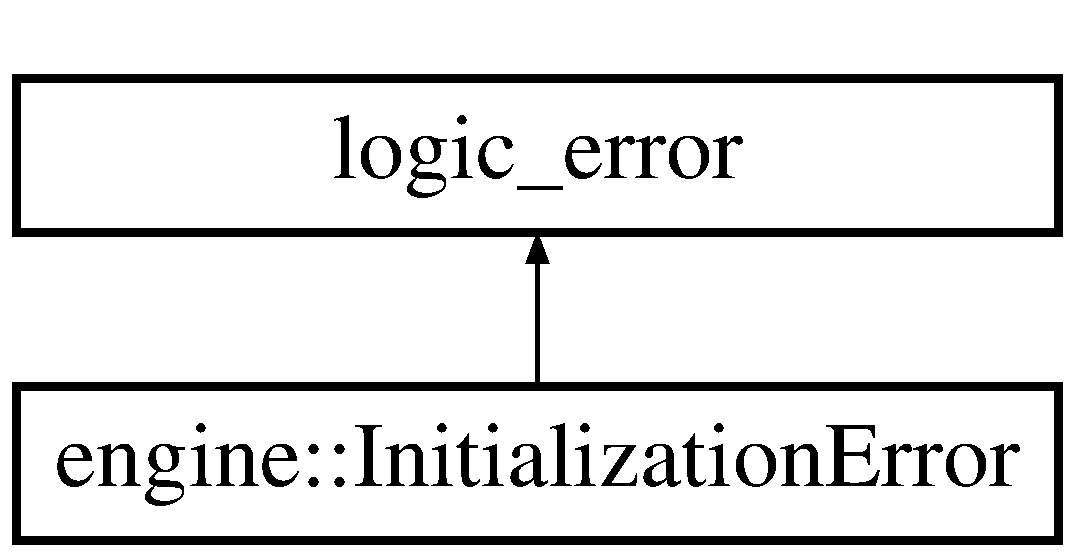
\includegraphics[height=2.000000cm]{a00048}
\end{center}
\end{figure}
\subsubsection*{Public Member Functions}
\begin{DoxyCompactItemize}
\item 
{\bfseries Initialization\+Error} (const std\+::string \&error)\hypertarget{a00048_a7292c661ed6737cf6a041176398e9893}{}\label{a00048_a7292c661ed6737cf6a041176398e9893}

\item 
{\bfseries Initialization\+Error} (const char $\ast$error)\hypertarget{a00048_a4313a4d837f17721d89740f940042eb2}{}\label{a00048_a4313a4d837f17721d89740f940042eb2}

\end{DoxyCompactItemize}


\subsubsection{Detailed Description}


Definition at line 7 of file Logical\+Errors.\+h.



The documentation for this struct was generated from the following file\+:\begin{DoxyCompactItemize}
\item 
E\+:/\+Programing/\+Projects/\+Engine\+Workspace/\+Common\+Libs/engine/include/engine/exceptions/Logical\+Errors.\+h\end{DoxyCompactItemize}

\hypertarget{a00049}{}\subsection{std\+:\+:is\+\_\+placeholder$<$ engine\+:\+:Custom\+Placeholder$<$ N $>$ $>$ Struct Template Reference}
\label{a00049}\index{std\+::is\+\_\+placeholder$<$ engine\+::\+Custom\+Placeholder$<$ N $>$ $>$@{std\+::is\+\_\+placeholder$<$ engine\+::\+Custom\+Placeholder$<$ N $>$ $>$}}


{\ttfamily \#include $<$E\+:/\+Programing/\+Projects/\+Engine\+Workspace/\+Common\+Libs/engine/include/engine/utils/\+Custom\+Placeholder.\+h$>$}

Inheritance diagram for std\+:\+:is\+\_\+placeholder$<$ engine\+:\+:Custom\+Placeholder$<$ N $>$ $>$\+:\begin{figure}[H]
\begin{center}
\leavevmode
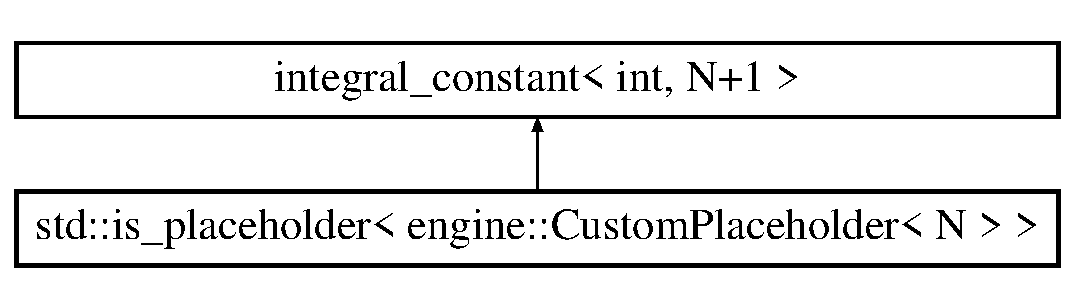
\includegraphics[height=2.000000cm]{a00049}
\end{center}
\end{figure}


\subsubsection{Detailed Description}
\subsubsection*{template$<$int N$>$\\*
struct std\+::is\+\_\+placeholder$<$ engine\+::\+Custom\+Placeholder$<$ N $>$ $>$}

Template specialization 

Definition at line 17 of file Custom\+Placeholder.\+h.



The documentation for this struct was generated from the following file\+:\begin{DoxyCompactItemize}
\item 
E\+:/\+Programing/\+Projects/\+Engine\+Workspace/\+Common\+Libs/engine/include/engine/utils/Custom\+Placeholder.\+h\end{DoxyCompactItemize}

\hypertarget{a00050}{}\subsection{engine\+:\+:I\+Signal Class Reference}
\label{a00050}\index{engine\+::\+I\+Signal@{engine\+::\+I\+Signal}}


{\ttfamily \#include $<$E\+:/\+Programing/\+Projects/\+Engine\+Workspace/\+Common\+Libs/engine/include/engine/signal\+Slot/\+I\+Signal.\+h$>$}

Inheritance diagram for engine\+:\+:I\+Signal\+:\begin{figure}[H]
\begin{center}
\leavevmode
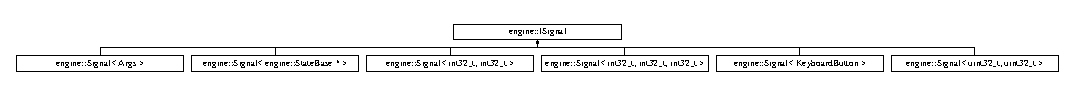
\includegraphics[height=0.740741cm]{a00050}
\end{center}
\end{figure}
\subsubsection*{Friends}
\begin{DoxyCompactItemize}
\item 
class {\bfseries Slot\+Holder}\hypertarget{a00050_a82af4fee1749e3f4e0b7c5eac6046ef5}{}\label{a00050_a82af4fee1749e3f4e0b7c5eac6046ef5}

\end{DoxyCompactItemize}


\subsubsection{Detailed Description}
Type independent signal 

Definition at line 9 of file I\+Signal.\+h.



The documentation for this class was generated from the following file\+:\begin{DoxyCompactItemize}
\item 
E\+:/\+Programing/\+Projects/\+Engine\+Workspace/\+Common\+Libs/engine/include/engine/signal\+Slot/I\+Signal.\+h\end{DoxyCompactItemize}

\hypertarget{a00051}{}\subsection{engine\+:\+:I\+Signal\+Manager Class Reference}
\label{a00051}\index{engine\+::\+I\+Signal\+Manager@{engine\+::\+I\+Signal\+Manager}}


{\ttfamily \#include $<$E\+:/\+Programing/\+Projects/\+Engine\+Workspace/\+Common\+Libs/engine/include/engine/signal\+Slot/\+I\+Signal\+Manager.\+h$>$}

Inheritance diagram for engine\+:\+:I\+Signal\+Manager\+:\begin{figure}[H]
\begin{center}
\leavevmode
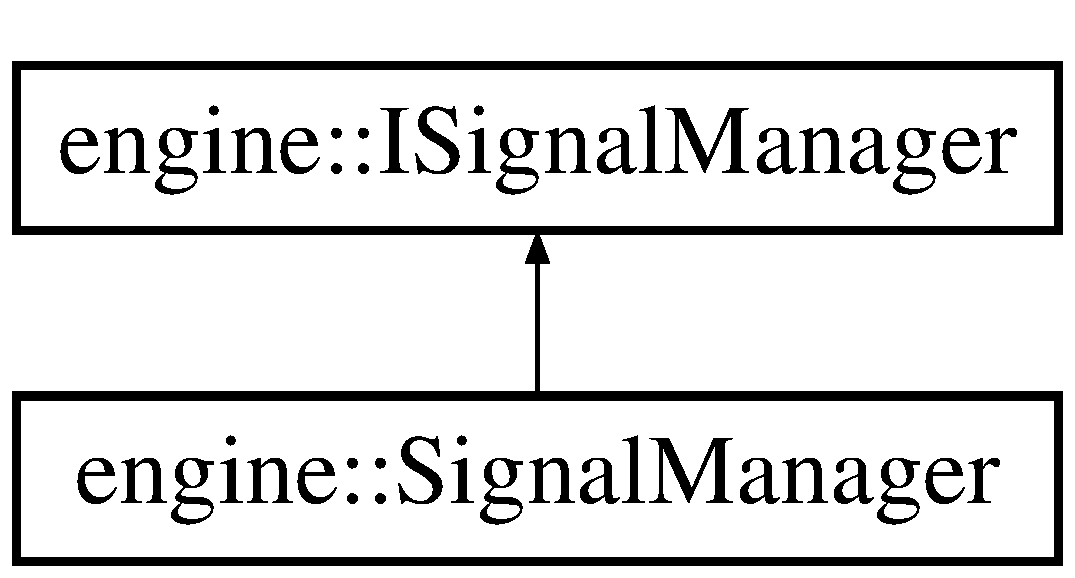
\includegraphics[height=2.000000cm]{a00051}
\end{center}
\end{figure}
\subsubsection*{Public Member Functions}
\begin{DoxyCompactItemize}
\item 
virtual \hyperlink{a00051_a96df44c1e1235d42d5632a5138d684e0}{$\sim$\+I\+Signal\+Manager} ()
\item 
virtual void \hyperlink{a00051_a45dd8b6dff3657f3538946bf1a8ea77c}{add\+Task} (std\+::unique\+\_\+ptr$<$ \hyperlink{a00052}{I\+Signal\+Task} $>$ task)=0
\item 
virtual void \hyperlink{a00051_ab28b704d755b789e6f88d7c30e2aa625}{update} ()=0
\end{DoxyCompactItemize}
\subsubsection*{Protected Member Functions}
\begin{DoxyCompactItemize}
\item 
\hyperlink{a00051_a2ff4db6b18c05b22db35c9d62bed82bc}{I\+Signal\+Manager} ()=default
\end{DoxyCompactItemize}


\subsubsection{Detailed Description}
Interface of the signal manager. Signals are created task during emit, this interface is responsible to manage these tasks. 

Definition at line 12 of file I\+Signal\+Manager.\+h.



\subsubsection{Constructor \& Destructor Documentation}
\index{engine\+::\+I\+Signal\+Manager@{engine\+::\+I\+Signal\+Manager}!I\+Signal\+Manager@{I\+Signal\+Manager}}
\index{I\+Signal\+Manager@{I\+Signal\+Manager}!engine\+::\+I\+Signal\+Manager@{engine\+::\+I\+Signal\+Manager}}
\paragraph[{\texorpdfstring{I\+Signal\+Manager()=default}{ISignalManager()=default}}]{\setlength{\rightskip}{0pt plus 5cm}engine\+::\+I\+Signal\+Manager\+::\+I\+Signal\+Manager (
\begin{DoxyParamCaption}
{}
\end{DoxyParamCaption}
)\hspace{0.3cm}{\ttfamily [protected]}, {\ttfamily [default]}}\hypertarget{a00051_a2ff4db6b18c05b22db35c9d62bed82bc}{}\label{a00051_a2ff4db6b18c05b22db35c9d62bed82bc}
Default constructor \index{engine\+::\+I\+Signal\+Manager@{engine\+::\+I\+Signal\+Manager}!````~I\+Signal\+Manager@{$\sim$\+I\+Signal\+Manager}}
\index{````~I\+Signal\+Manager@{$\sim$\+I\+Signal\+Manager}!engine\+::\+I\+Signal\+Manager@{engine\+::\+I\+Signal\+Manager}}
\paragraph[{\texorpdfstring{$\sim$\+I\+Signal\+Manager()}{~ISignalManager()}}]{\setlength{\rightskip}{0pt plus 5cm}virtual engine\+::\+I\+Signal\+Manager\+::$\sim$\+I\+Signal\+Manager (
\begin{DoxyParamCaption}
{}
\end{DoxyParamCaption}
)\hspace{0.3cm}{\ttfamily [inline]}, {\ttfamily [virtual]}}\hypertarget{a00051_a96df44c1e1235d42d5632a5138d684e0}{}\label{a00051_a96df44c1e1235d42d5632a5138d684e0}
Default destructor 

Definition at line 19 of file I\+Signal\+Manager.\+h.



\subsubsection{Member Function Documentation}
\index{engine\+::\+I\+Signal\+Manager@{engine\+::\+I\+Signal\+Manager}!add\+Task@{add\+Task}}
\index{add\+Task@{add\+Task}!engine\+::\+I\+Signal\+Manager@{engine\+::\+I\+Signal\+Manager}}
\paragraph[{\texorpdfstring{add\+Task(std\+::unique\+\_\+ptr$<$ I\+Signal\+Task $>$ task)=0}{addTask(std::unique_ptr< ISignalTask > task)=0}}]{\setlength{\rightskip}{0pt plus 5cm}virtual void engine\+::\+I\+Signal\+Manager\+::add\+Task (
\begin{DoxyParamCaption}
\item[{std\+::unique\+\_\+ptr$<$ {\bf I\+Signal\+Task} $>$}]{task}
\end{DoxyParamCaption}
)\hspace{0.3cm}{\ttfamily [pure virtual]}}\hypertarget{a00051_a45dd8b6dff3657f3538946bf1a8ea77c}{}\label{a00051_a45dd8b6dff3657f3538946bf1a8ea77c}
Assign a task to the manager. It\textquotesingle{}s called when a task is emitted. 

Implemented in \hyperlink{a00067_a5ac2136c91ad2e8a5e912f3f906d0073}{engine\+::\+Signal\+Manager}.



Referenced by $\sim$\+I\+Signal\+Manager().

\index{engine\+::\+I\+Signal\+Manager@{engine\+::\+I\+Signal\+Manager}!update@{update}}
\index{update@{update}!engine\+::\+I\+Signal\+Manager@{engine\+::\+I\+Signal\+Manager}}
\paragraph[{\texorpdfstring{update()=0}{update()=0}}]{\setlength{\rightskip}{0pt plus 5cm}virtual void engine\+::\+I\+Signal\+Manager\+::update (
\begin{DoxyParamCaption}
{}
\end{DoxyParamCaption}
)\hspace{0.3cm}{\ttfamily [pure virtual]}}\hypertarget{a00051_ab28b704d755b789e6f88d7c30e2aa625}{}\label{a00051_ab28b704d755b789e6f88d7c30e2aa625}
Update the manager. It\textquotesingle{}s for manage the tasks of the assigned manager. 

Implemented in \hyperlink{a00067_a4e2dbe6e08226abfca06f172606b102b}{engine\+::\+Signal\+Manager}.



Referenced by $\sim$\+I\+Signal\+Manager().



The documentation for this class was generated from the following file\+:\begin{DoxyCompactItemize}
\item 
E\+:/\+Programing/\+Projects/\+Engine\+Workspace/\+Common\+Libs/engine/include/engine/signal\+Slot/I\+Signal\+Manager.\+h\end{DoxyCompactItemize}

\hypertarget{a00052}{}\subsection{engine\+:\+:I\+Signal\+Task Class Reference}
\label{a00052}\index{engine\+::\+I\+Signal\+Task@{engine\+::\+I\+Signal\+Task}}


{\ttfamily \#include $<$E\+:/\+Programing/\+Projects/\+Engine\+Workspace/\+Common\+Libs/engine/include/engine/signal\+Slot/\+Signal\+Task.\+h$>$}

Inheritance diagram for engine\+:\+:I\+Signal\+Task\+:\begin{figure}[H]
\begin{center}
\leavevmode
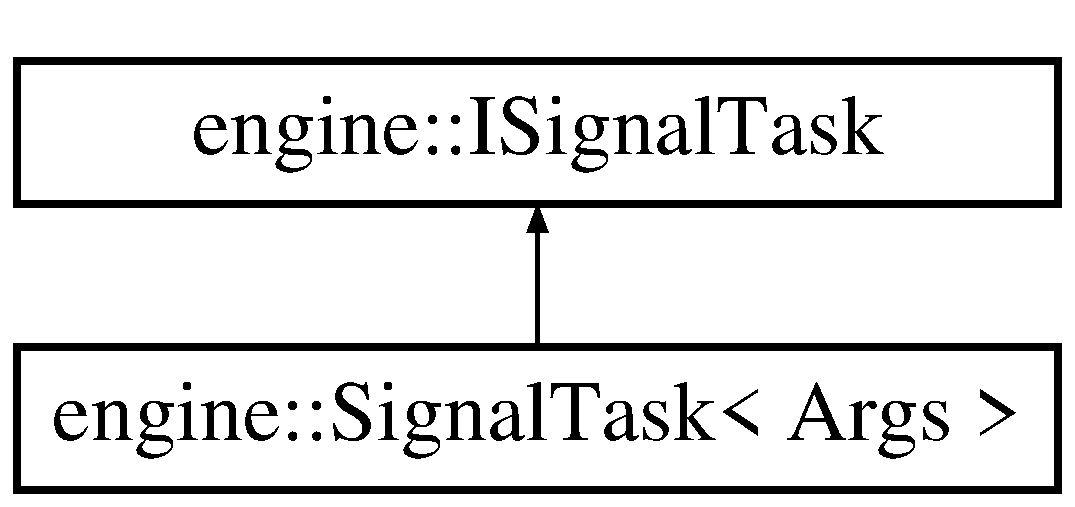
\includegraphics[height=2.000000cm]{a00052}
\end{center}
\end{figure}
\subsubsection*{Public Member Functions}
\begin{DoxyCompactItemize}
\item 
virtual \hyperlink{a00052_a8f7c6610cc8bfd5249d3b391c6efc95b}{$\sim$\+I\+Signal\+Task} ()
\item 
virtual void \hyperlink{a00052_ab7e5dedd50f908fdb0f203b0a154db54}{operator()} ()=0
\item 
virtual bool \hyperlink{a00052_aaa397480f1ad28755a63ad1dca559d50}{is\+Expired} () const  =0
\end{DoxyCompactItemize}


\subsubsection{Detailed Description}
Task which is created from a slot and a given member 

Definition at line 10 of file Signal\+Task.\+h.



\subsubsection{Constructor \& Destructor Documentation}
\index{engine\+::\+I\+Signal\+Task@{engine\+::\+I\+Signal\+Task}!````~I\+Signal\+Task@{$\sim$\+I\+Signal\+Task}}
\index{````~I\+Signal\+Task@{$\sim$\+I\+Signal\+Task}!engine\+::\+I\+Signal\+Task@{engine\+::\+I\+Signal\+Task}}
\paragraph[{\texorpdfstring{$\sim$\+I\+Signal\+Task()}{~ISignalTask()}}]{\setlength{\rightskip}{0pt plus 5cm}virtual engine\+::\+I\+Signal\+Task\+::$\sim$\+I\+Signal\+Task (
\begin{DoxyParamCaption}
{}
\end{DoxyParamCaption}
)\hspace{0.3cm}{\ttfamily [inline]}, {\ttfamily [virtual]}}\hypertarget{a00052_a8f7c6610cc8bfd5249d3b391c6efc95b}{}\label{a00052_a8f7c6610cc8bfd5249d3b391c6efc95b}
Default destructor 

Definition at line 14 of file Signal\+Task.\+h.



\subsubsection{Member Function Documentation}
\index{engine\+::\+I\+Signal\+Task@{engine\+::\+I\+Signal\+Task}!is\+Expired@{is\+Expired}}
\index{is\+Expired@{is\+Expired}!engine\+::\+I\+Signal\+Task@{engine\+::\+I\+Signal\+Task}}
\paragraph[{\texorpdfstring{is\+Expired() const  =0}{isExpired() const  =0}}]{\setlength{\rightskip}{0pt plus 5cm}virtual bool engine\+::\+I\+Signal\+Task\+::is\+Expired (
\begin{DoxyParamCaption}
{}
\end{DoxyParamCaption}
) const\hspace{0.3cm}{\ttfamily [pure virtual]}}\hypertarget{a00052_aaa397480f1ad28755a63ad1dca559d50}{}\label{a00052_aaa397480f1ad28755a63ad1dca559d50}
Expired if the \hyperlink{a00066}{Signal\+Caller} has been destroyed. 

Implemented in \hyperlink{a00068_af923108f7304a686bc4b7eeb41c35177}{engine\+::\+Signal\+Task$<$ Args $>$}.



Referenced by engine\+::\+Signal\+Task$<$ Args $>$\+::operator()(), and $\sim$\+I\+Signal\+Task().

\index{engine\+::\+I\+Signal\+Task@{engine\+::\+I\+Signal\+Task}!operator()@{operator()}}
\index{operator()@{operator()}!engine\+::\+I\+Signal\+Task@{engine\+::\+I\+Signal\+Task}}
\paragraph[{\texorpdfstring{operator()()=0}{operator()()=0}}]{\setlength{\rightskip}{0pt plus 5cm}virtual void engine\+::\+I\+Signal\+Task\+::operator() (
\begin{DoxyParamCaption}
{}
\end{DoxyParamCaption}
)\hspace{0.3cm}{\ttfamily [pure virtual]}}\hypertarget{a00052_ab7e5dedd50f908fdb0f203b0a154db54}{}\label{a00052_ab7e5dedd50f908fdb0f203b0a154db54}
Execute the slot 

Implemented in \hyperlink{a00068_a66e71dfc80f4320c2d5c260028b0bbff}{engine\+::\+Signal\+Task$<$ Args $>$}.



Referenced by $\sim$\+I\+Signal\+Task().



The documentation for this class was generated from the following file\+:\begin{DoxyCompactItemize}
\item 
E\+:/\+Programing/\+Projects/\+Engine\+Workspace/\+Common\+Libs/engine/include/engine/signal\+Slot/Signal\+Task.\+h\end{DoxyCompactItemize}

\hypertarget{a00053}{}\subsection{engine\+:\+:Item\+Not\+Found Struct Reference}
\label{a00053}\index{engine\+::\+Item\+Not\+Found@{engine\+::\+Item\+Not\+Found}}
Inheritance diagram for engine\+:\+:Item\+Not\+Found\+:\begin{figure}[H]
\begin{center}
\leavevmode
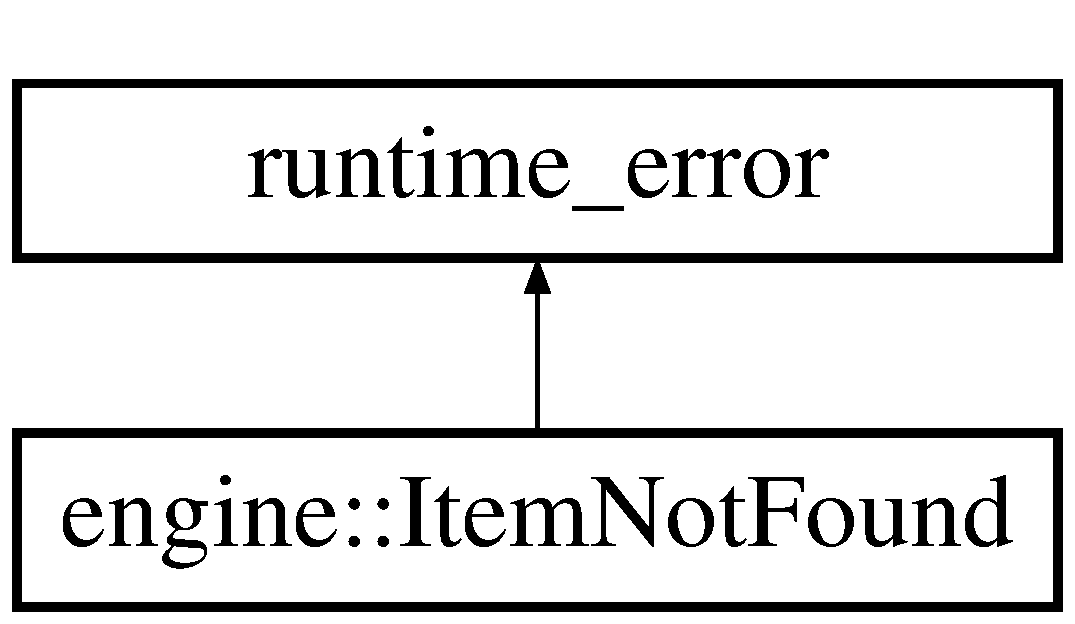
\includegraphics[height=2.000000cm]{a00053}
\end{center}
\end{figure}
\subsubsection*{Public Member Functions}
\begin{DoxyCompactItemize}
\item 
{\bfseries Item\+Not\+Found} (const std\+::string \&error)\hypertarget{a00053_aee33918da6da193cf1f05d7941b94bd9}{}\label{a00053_aee33918da6da193cf1f05d7941b94bd9}

\item 
{\bfseries Item\+Not\+Found} (const char $\ast$error)\hypertarget{a00053_a030ba329518781adcfe162b839ec4348}{}\label{a00053_a030ba329518781adcfe162b839ec4348}

\end{DoxyCompactItemize}


\subsubsection{Detailed Description}


Definition at line 18 of file Runtime\+Errors.\+h.



The documentation for this struct was generated from the following file\+:\begin{DoxyCompactItemize}
\item 
E\+:/\+Programing/\+Projects/\+Engine\+Workspace/\+Common\+Libs/engine/include/engine/exceptions/Runtime\+Errors.\+h\end{DoxyCompactItemize}

\hypertarget{a00054}{}\subsection{engine\+:\+:test\+:\+:I\+Test\+Case Class Reference}
\label{a00054}\index{engine\+::test\+::\+I\+Test\+Case@{engine\+::test\+::\+I\+Test\+Case}}
Inheritance diagram for engine\+:\+:test\+:\+:I\+Test\+Case\+:\begin{figure}[H]
\begin{center}
\leavevmode
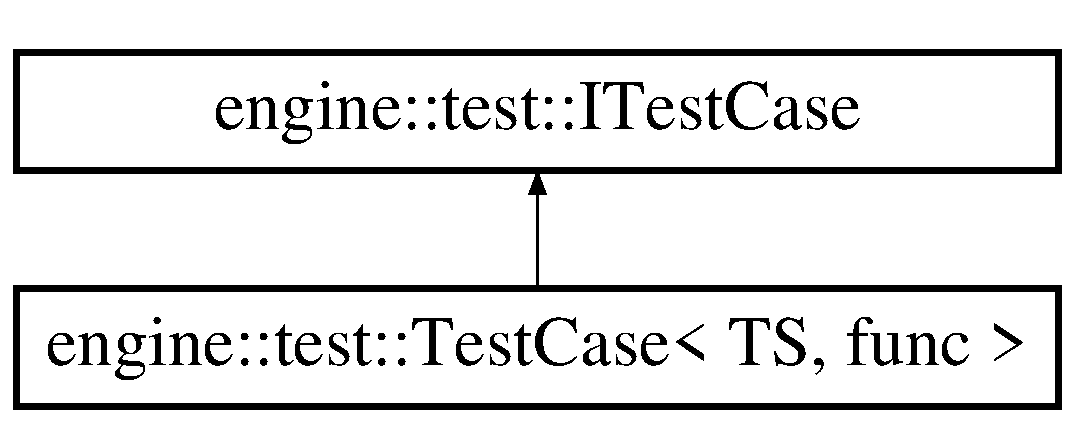
\includegraphics[height=2.000000cm]{a00054}
\end{center}
\end{figure}
\subsubsection*{Public Member Functions}
\begin{DoxyCompactItemize}
\item 
virtual void {\bfseries execute} ()=0\hypertarget{a00054_a7e50dee56c82bb195fd99c1137fd657c}{}\label{a00054_a7e50dee56c82bb195fd99c1137fd657c}

\item 
virtual const std\+::string \& {\bfseries get\+Name} () const  =0\hypertarget{a00054_a224b4ed84824c244fbc68400f9e45eca}{}\label{a00054_a224b4ed84824c244fbc68400f9e45eca}

\end{DoxyCompactItemize}


\subsubsection{Detailed Description}


Definition at line 7 of file I\+Test\+Case.\+h.



The documentation for this class was generated from the following file\+:\begin{DoxyCompactItemize}
\item 
E\+:/\+Programing/\+Projects/\+Engine\+Workspace/\+Common\+Libs/engine/include/engine/test/I\+Test\+Case.\+h\end{DoxyCompactItemize}

\hypertarget{a00055}{}\subsection{engine\+:\+:Keyboard Class Reference}
\label{a00055}\index{engine\+::\+Keyboard@{engine\+::\+Keyboard}}
Inheritance diagram for engine\+:\+:Keyboard\+:\begin{figure}[H]
\begin{center}
\leavevmode
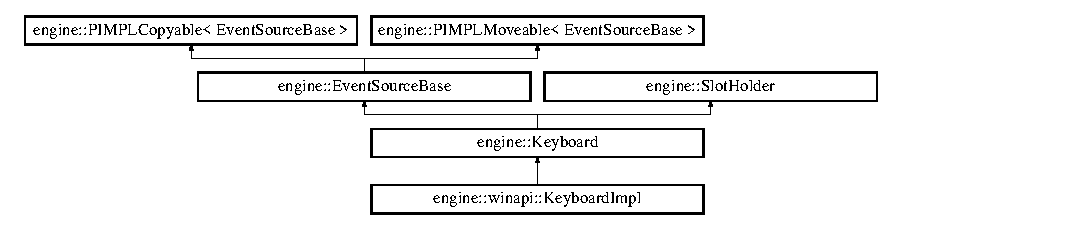
\includegraphics[height=2.647754cm]{a00055}
\end{center}
\end{figure}
\subsubsection*{Public Member Functions}
\begin{DoxyCompactItemize}
\item 
{\bfseries Keyboard} (\hyperlink{a00055}{Keyboard} \&\&o)\hypertarget{a00055_ad4410c745ee235f4418feb55656f59e2}{}\label{a00055_ad4410c745ee235f4418feb55656f59e2}

\item 
\hyperlink{a00055}{Keyboard} \& {\bfseries operator=} (\hyperlink{a00055}{Keyboard} \&\&o)\hypertarget{a00055_acbdb16f8b16fe00da53eab07736f6364}{}\label{a00055_acbdb16f8b16fe00da53eab07736f6364}

\item 
Key\+State {\bfseries get\+Key\+State} (Keyboard\+Button button) const \hypertarget{a00055_a89fd597ce678be8a6b50a36b549a5922}{}\label{a00055_a89fd597ce678be8a6b50a36b549a5922}

\item 
\hyperlink{a00051}{I\+Signal\+Manager} $\ast$ \hyperlink{a00055_a324f41177f75c6d08ad6494c36a65806}{get\+Signal\+Manager} () const  override
\item 
void {\bfseries set\+Events\+Enabled} (bool v)\hypertarget{a00036_ae529242181c16462bef9bd6b8fb56b93}{}\label{a00036_ae529242181c16462bef9bd6b8fb56b93}

\item 
bool {\bfseries is\+Events\+Enabled} () const \hypertarget{a00036_a659325f18d666f132f380e4319499572}{}\label{a00036_a659325f18d666f132f380e4319499572}

\item 
const std\+::string \& {\bfseries get\+Event\+Source\+Id} () const \hypertarget{a00036_ad41deeb2b9de38797b10777e5d1ecf13}{}\label{a00036_ad41deeb2b9de38797b10777e5d1ecf13}

\item 
\hyperlink{a00036}{Event\+Source\+Base} \& {\bfseries P\+I\+M\+P\+L\+Copyable\+::operator=} (const \hyperlink{a00060}{P\+I\+M\+P\+L\+Copyable} \&o)\hypertarget{a00060_a26fdb9b3d449d04dc653c7ae942f452b}{}\label{a00060_a26fdb9b3d449d04dc653c7ae942f452b}

\item 
\hyperlink{a00036}{Event\+Source\+Base} \& {\bfseries P\+I\+M\+P\+L\+Moveable\+::operator=} (\hyperlink{a00061}{P\+I\+M\+P\+L\+Moveable} \&\&o)\hypertarget{a00061_ac67025e8a25edffe99fa9bf67ed8ca19}{}\label{a00061_ac67025e8a25edffe99fa9bf67ed8ca19}

\item 
void \hyperlink{a00070_afd9ce54a72b4dd397d82aff6c387d0c0}{assign\+Signal} (\hyperlink{a00050}{I\+Signal} $\ast$signal)
\item 
void \hyperlink{a00070_a5927b57f0d4fb8744dc0e8ec265e0136}{remove\+Signal} (\hyperlink{a00050}{I\+Signal} $\ast$signal)
\end{DoxyCompactItemize}
\subsubsection*{Static Public Member Functions}
\begin{DoxyCompactItemize}
\item 
static std\+::string {\bfseries Keyboard\+Button\+To\+String} (Keyboard\+Button button)\hypertarget{a00055_a4204702d8f964a109136545690686585}{}\label{a00055_a4204702d8f964a109136545690686585}

\end{DoxyCompactItemize}
\subsubsection*{Public Attributes}
\begin{DoxyCompactItemize}
\item 
\hyperlink{a00065}{Signal}$<$ Keyboard\+Button $>$ {\bfseries key\+Pressed}\hypertarget{a00055_a96ef16f70810ff3ceffde1ad71f9291f}{}\label{a00055_a96ef16f70810ff3ceffde1ad71f9291f}

\item 
\hyperlink{a00065}{Signal}$<$ Keyboard\+Button $>$ {\bfseries key\+Released}\hypertarget{a00055_a081464fd7756415ad9c78e80e850cbea}{}\label{a00055_a081464fd7756415ad9c78e80e850cbea}

\end{DoxyCompactItemize}
\subsubsection*{Static Public Attributes}
\begin{DoxyCompactItemize}
\item 
static const std\+::string {\bfseries Event\+Source\+Id}\hypertarget{a00055_a11ae52b8b6e7519d0b3ea42561d6dccd}{}\label{a00055_a11ae52b8b6e7519d0b3ea42561d6dccd}

\end{DoxyCompactItemize}
\subsubsection*{Protected Member Functions}
\begin{DoxyCompactItemize}
\item 
void {\bfseries on\+Key\+Pressed} (Keyboard\+Button)\hypertarget{a00055_a5072ad733814bd17d46e36ea8be4a4b4}{}\label{a00055_a5072ad733814bd17d46e36ea8be4a4b4}

\item 
void {\bfseries on\+Key\+Released} (Keyboard\+Button)\hypertarget{a00055_a000acdad189778380e4ac141dd4619cb}{}\label{a00055_a000acdad189778380e4ac141dd4619cb}

\end{DoxyCompactItemize}


\subsubsection{Detailed Description}


Definition at line 135 of file Keyboard.\+h.



\subsubsection{Member Function Documentation}
\index{engine\+::\+Keyboard@{engine\+::\+Keyboard}!assign\+Signal@{assign\+Signal}}
\index{assign\+Signal@{assign\+Signal}!engine\+::\+Keyboard@{engine\+::\+Keyboard}}
\paragraph[{\texorpdfstring{assign\+Signal(\+I\+Signal $\ast$signal)}{assignSignal(ISignal *signal)}}]{\setlength{\rightskip}{0pt plus 5cm}void engine\+::\+Slot\+Holder\+::assign\+Signal (
\begin{DoxyParamCaption}
\item[{{\bf I\+Signal} $\ast$}]{signal}
\end{DoxyParamCaption}
)\hspace{0.3cm}{\ttfamily [inherited]}}\hypertarget{a00070_afd9ce54a72b4dd397d82aff6c387d0c0}{}\label{a00070_afd9ce54a72b4dd397d82aff6c387d0c0}
Assign a signal to this slot. It is necessery because when this object is destroyed, it must tell to the signal that\textquotesingle{}s not alived. \index{engine\+::\+Keyboard@{engine\+::\+Keyboard}!get\+Signal\+Manager@{get\+Signal\+Manager}}
\index{get\+Signal\+Manager@{get\+Signal\+Manager}!engine\+::\+Keyboard@{engine\+::\+Keyboard}}
\paragraph[{\texorpdfstring{get\+Signal\+Manager() const  override}{getSignalManager() const  override}}]{\setlength{\rightskip}{0pt plus 5cm}{\bf I\+Signal\+Manager}$\ast$ engine\+::\+Keyboard\+::get\+Signal\+Manager (
\begin{DoxyParamCaption}
{}
\end{DoxyParamCaption}
) const\hspace{0.3cm}{\ttfamily [override]}, {\ttfamily [virtual]}}\hypertarget{a00055_a324f41177f75c6d08ad6494c36a65806}{}\label{a00055_a324f41177f75c6d08ad6494c36a65806}
\begin{DoxyReturn}{Returns}
Returns the corresponding \hyperlink{a00067}{Signal\+Manager}, who will manage the tasks. 
\end{DoxyReturn}


Implements \hyperlink{a00070_add6d89f31a2677b29a52f241d0431c13}{engine\+::\+Slot\+Holder}.

\index{engine\+::\+Keyboard@{engine\+::\+Keyboard}!remove\+Signal@{remove\+Signal}}
\index{remove\+Signal@{remove\+Signal}!engine\+::\+Keyboard@{engine\+::\+Keyboard}}
\paragraph[{\texorpdfstring{remove\+Signal(\+I\+Signal $\ast$signal)}{removeSignal(ISignal *signal)}}]{\setlength{\rightskip}{0pt plus 5cm}void engine\+::\+Slot\+Holder\+::remove\+Signal (
\begin{DoxyParamCaption}
\item[{{\bf I\+Signal} $\ast$}]{signal}
\end{DoxyParamCaption}
)\hspace{0.3cm}{\ttfamily [inherited]}}\hypertarget{a00070_a5927b57f0d4fb8744dc0e8ec265e0136}{}\label{a00070_a5927b57f0d4fb8744dc0e8ec265e0136}
Remove signal from this slots. 

The documentation for this class was generated from the following file\+:\begin{DoxyCompactItemize}
\item 
E\+:/\+Programing/\+Projects/\+Engine\+Workspace/\+Common\+Libs/engine/include/engine/events/Keyboard.\+h\end{DoxyCompactItemize}

\hypertarget{a00056}{}\subsection{engine\+:\+:winapi\+:\+:Keyboard\+Impl Class Reference}
\label{a00056}\index{engine\+::winapi\+::\+Keyboard\+Impl@{engine\+::winapi\+::\+Keyboard\+Impl}}
Inheritance diagram for engine\+:\+:winapi\+:\+:Keyboard\+Impl\+:\begin{figure}[H]
\begin{center}
\leavevmode
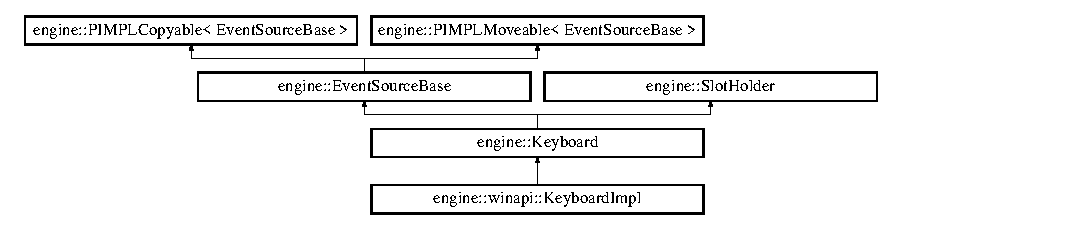
\includegraphics[height=2.647754cm]{a00056}
\end{center}
\end{figure}
\subsubsection*{Public Member Functions}
\begin{DoxyCompactItemize}
\item 
bool {\bfseries handle\+Event} (H\+W\+ND h\+Wnd, U\+I\+NT message, W\+P\+A\+R\+AM w\+Param, L\+P\+A\+R\+AM l\+Param)\hypertarget{a00056_a71dec63b611c18f3ea41c8fdebc81191}{}\label{a00056_a71dec63b611c18f3ea41c8fdebc81191}

\item 
Key\+State {\bfseries get\+Key\+State} (Keyboard\+Button button) const \hypertarget{a00055_a89fd597ce678be8a6b50a36b549a5922}{}\label{a00055_a89fd597ce678be8a6b50a36b549a5922}

\item 
\hyperlink{a00051}{I\+Signal\+Manager} $\ast$ \hyperlink{a00055_a324f41177f75c6d08ad6494c36a65806}{get\+Signal\+Manager} () const  override
\item 
void {\bfseries set\+Events\+Enabled} (bool v)\hypertarget{a00036_ae529242181c16462bef9bd6b8fb56b93}{}\label{a00036_ae529242181c16462bef9bd6b8fb56b93}

\item 
bool {\bfseries is\+Events\+Enabled} () const \hypertarget{a00036_a659325f18d666f132f380e4319499572}{}\label{a00036_a659325f18d666f132f380e4319499572}

\item 
const std\+::string \& {\bfseries get\+Event\+Source\+Id} () const \hypertarget{a00036_ad41deeb2b9de38797b10777e5d1ecf13}{}\label{a00036_ad41deeb2b9de38797b10777e5d1ecf13}

\item 
\hyperlink{a00036}{Event\+Source\+Base} \& {\bfseries P\+I\+M\+P\+L\+Copyable\+::operator=} (const \hyperlink{a00060}{P\+I\+M\+P\+L\+Copyable} \&o)\hypertarget{a00060_a26fdb9b3d449d04dc653c7ae942f452b}{}\label{a00060_a26fdb9b3d449d04dc653c7ae942f452b}

\item 
\hyperlink{a00036}{Event\+Source\+Base} \& {\bfseries P\+I\+M\+P\+L\+Moveable\+::operator=} (\hyperlink{a00061}{P\+I\+M\+P\+L\+Moveable} \&\&o)\hypertarget{a00061_ac67025e8a25edffe99fa9bf67ed8ca19}{}\label{a00061_ac67025e8a25edffe99fa9bf67ed8ca19}

\item 
void \hyperlink{a00070_afd9ce54a72b4dd397d82aff6c387d0c0}{assign\+Signal} (\hyperlink{a00050}{I\+Signal} $\ast$signal)
\item 
void \hyperlink{a00070_a5927b57f0d4fb8744dc0e8ec265e0136}{remove\+Signal} (\hyperlink{a00050}{I\+Signal} $\ast$signal)
\end{DoxyCompactItemize}
\subsubsection*{Static Public Member Functions}
\begin{DoxyCompactItemize}
\item 
static std\+::string {\bfseries Keyboard\+Button\+To\+String} (Keyboard\+Button button)\hypertarget{a00055_a4204702d8f964a109136545690686585}{}\label{a00055_a4204702d8f964a109136545690686585}

\end{DoxyCompactItemize}
\subsubsection*{Public Attributes}
\begin{DoxyCompactItemize}
\item 
\hyperlink{a00065}{Signal}$<$ Keyboard\+Button $>$ {\bfseries key\+Pressed}\hypertarget{a00055_a96ef16f70810ff3ceffde1ad71f9291f}{}\label{a00055_a96ef16f70810ff3ceffde1ad71f9291f}

\item 
\hyperlink{a00065}{Signal}$<$ Keyboard\+Button $>$ {\bfseries key\+Released}\hypertarget{a00055_a081464fd7756415ad9c78e80e850cbea}{}\label{a00055_a081464fd7756415ad9c78e80e850cbea}

\end{DoxyCompactItemize}
\subsubsection*{Static Public Attributes}
\begin{DoxyCompactItemize}
\item 
static const std\+::string {\bfseries Event\+Source\+Id}\hypertarget{a00055_a11ae52b8b6e7519d0b3ea42561d6dccd}{}\label{a00055_a11ae52b8b6e7519d0b3ea42561d6dccd}

\end{DoxyCompactItemize}
\subsubsection*{Protected Member Functions}
\begin{DoxyCompactItemize}
\item 
void {\bfseries on\+Key\+Pressed} (Keyboard\+Button)\hypertarget{a00055_a5072ad733814bd17d46e36ea8be4a4b4}{}\label{a00055_a5072ad733814bd17d46e36ea8be4a4b4}

\item 
void {\bfseries on\+Key\+Released} (Keyboard\+Button)\hypertarget{a00055_a000acdad189778380e4ac141dd4619cb}{}\label{a00055_a000acdad189778380e4ac141dd4619cb}

\end{DoxyCompactItemize}


\subsubsection{Detailed Description}


Definition at line 11 of file Keyboard\+Impl.\+h.



\subsubsection{Member Function Documentation}
\index{engine\+::winapi\+::\+Keyboard\+Impl@{engine\+::winapi\+::\+Keyboard\+Impl}!assign\+Signal@{assign\+Signal}}
\index{assign\+Signal@{assign\+Signal}!engine\+::winapi\+::\+Keyboard\+Impl@{engine\+::winapi\+::\+Keyboard\+Impl}}
\paragraph[{\texorpdfstring{assign\+Signal(\+I\+Signal $\ast$signal)}{assignSignal(ISignal *signal)}}]{\setlength{\rightskip}{0pt plus 5cm}void engine\+::\+Slot\+Holder\+::assign\+Signal (
\begin{DoxyParamCaption}
\item[{{\bf I\+Signal} $\ast$}]{signal}
\end{DoxyParamCaption}
)\hspace{0.3cm}{\ttfamily [inherited]}}\hypertarget{a00070_afd9ce54a72b4dd397d82aff6c387d0c0}{}\label{a00070_afd9ce54a72b4dd397d82aff6c387d0c0}
Assign a signal to this slot. It is necessery because when this object is destroyed, it must tell to the signal that\textquotesingle{}s not alived. \index{engine\+::winapi\+::\+Keyboard\+Impl@{engine\+::winapi\+::\+Keyboard\+Impl}!get\+Signal\+Manager@{get\+Signal\+Manager}}
\index{get\+Signal\+Manager@{get\+Signal\+Manager}!engine\+::winapi\+::\+Keyboard\+Impl@{engine\+::winapi\+::\+Keyboard\+Impl}}
\paragraph[{\texorpdfstring{get\+Signal\+Manager() const  override}{getSignalManager() const  override}}]{\setlength{\rightskip}{0pt plus 5cm}{\bf I\+Signal\+Manager}$\ast$ engine\+::\+Keyboard\+::get\+Signal\+Manager (
\begin{DoxyParamCaption}
{}
\end{DoxyParamCaption}
) const\hspace{0.3cm}{\ttfamily [override]}, {\ttfamily [virtual]}, {\ttfamily [inherited]}}\hypertarget{a00055_a324f41177f75c6d08ad6494c36a65806}{}\label{a00055_a324f41177f75c6d08ad6494c36a65806}
\begin{DoxyReturn}{Returns}
Returns the corresponding \hyperlink{a00067}{Signal\+Manager}, who will manage the tasks. 
\end{DoxyReturn}


Implements \hyperlink{a00070_add6d89f31a2677b29a52f241d0431c13}{engine\+::\+Slot\+Holder}.

\index{engine\+::winapi\+::\+Keyboard\+Impl@{engine\+::winapi\+::\+Keyboard\+Impl}!remove\+Signal@{remove\+Signal}}
\index{remove\+Signal@{remove\+Signal}!engine\+::winapi\+::\+Keyboard\+Impl@{engine\+::winapi\+::\+Keyboard\+Impl}}
\paragraph[{\texorpdfstring{remove\+Signal(\+I\+Signal $\ast$signal)}{removeSignal(ISignal *signal)}}]{\setlength{\rightskip}{0pt plus 5cm}void engine\+::\+Slot\+Holder\+::remove\+Signal (
\begin{DoxyParamCaption}
\item[{{\bf I\+Signal} $\ast$}]{signal}
\end{DoxyParamCaption}
)\hspace{0.3cm}{\ttfamily [inherited]}}\hypertarget{a00070_a5927b57f0d4fb8744dc0e8ec265e0136}{}\label{a00070_a5927b57f0d4fb8744dc0e8ec265e0136}
Remove signal from this slots. 

The documentation for this class was generated from the following file\+:\begin{DoxyCompactItemize}
\item 
E\+:/\+Programing/\+Projects/\+Engine\+Workspace/\+Common\+Libs/engine/include/engine/events/winapi/Keyboard\+Impl.\+h\end{DoxyCompactItemize}

\hypertarget{a00057}{}\subsection{engine\+:\+:Mouse Class Reference}
\label{a00057}\index{engine\+::\+Mouse@{engine\+::\+Mouse}}
Inheritance diagram for engine\+:\+:Mouse\+:\begin{figure}[H]
\begin{center}
\leavevmode
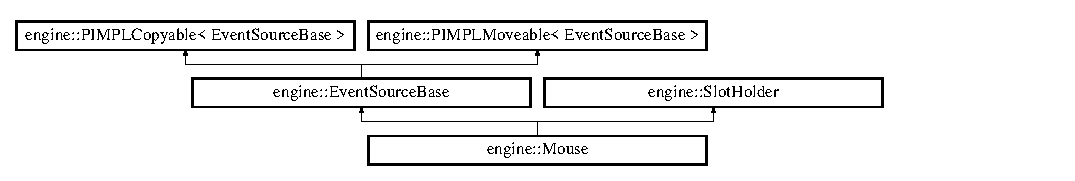
\includegraphics[height=1.985816cm]{a00057}
\end{center}
\end{figure}
\subsubsection*{Public Member Functions}
\begin{DoxyCompactItemize}
\item 
Mouse\+Button\+State {\bfseries get\+Button\+State} (Mouse\+Button) const \hypertarget{a00057_a91c3072a154c629723e7fb83ea58c453}{}\label{a00057_a91c3072a154c629723e7fb83ea58c453}

\item 
\hyperlink{a00051}{I\+Signal\+Manager} $\ast$ \hyperlink{a00057_a655d612dbf601fec2b116a1c94198247}{get\+Signal\+Manager} () const  override
\item 
void {\bfseries set\+Events\+Enabled} (bool v)\hypertarget{a00036_ae529242181c16462bef9bd6b8fb56b93}{}\label{a00036_ae529242181c16462bef9bd6b8fb56b93}

\item 
bool {\bfseries is\+Events\+Enabled} () const \hypertarget{a00036_a659325f18d666f132f380e4319499572}{}\label{a00036_a659325f18d666f132f380e4319499572}

\item 
const std\+::string \& {\bfseries get\+Event\+Source\+Id} () const \hypertarget{a00036_ad41deeb2b9de38797b10777e5d1ecf13}{}\label{a00036_ad41deeb2b9de38797b10777e5d1ecf13}

\item 
\hyperlink{a00036}{Event\+Source\+Base} \& {\bfseries P\+I\+M\+P\+L\+Copyable\+::operator=} (const \hyperlink{a00060}{P\+I\+M\+P\+L\+Copyable} \&o)\hypertarget{a00060_a26fdb9b3d449d04dc653c7ae942f452b}{}\label{a00060_a26fdb9b3d449d04dc653c7ae942f452b}

\item 
\hyperlink{a00036}{Event\+Source\+Base} \& {\bfseries P\+I\+M\+P\+L\+Moveable\+::operator=} (\hyperlink{a00061}{P\+I\+M\+P\+L\+Moveable} \&\&o)\hypertarget{a00061_ac67025e8a25edffe99fa9bf67ed8ca19}{}\label{a00061_ac67025e8a25edffe99fa9bf67ed8ca19}

\item 
void \hyperlink{a00070_afd9ce54a72b4dd397d82aff6c387d0c0}{assign\+Signal} (\hyperlink{a00050}{I\+Signal} $\ast$signal)
\item 
void \hyperlink{a00070_a5927b57f0d4fb8744dc0e8ec265e0136}{remove\+Signal} (\hyperlink{a00050}{I\+Signal} $\ast$signal)
\end{DoxyCompactItemize}
\subsubsection*{Public Attributes}
\begin{DoxyCompactItemize}
\item 
\hyperlink{a00065}{Signal}$<$ int32\+\_\+t, int32\+\_\+t $>$ {\bfseries moved}\hypertarget{a00057_a2f8435311a86e43ce712428068be4388}{}\label{a00057_a2f8435311a86e43ce712428068be4388}

\item 
\hyperlink{a00065}{Signal}$<$ int32\+\_\+t, int32\+\_\+t $>$ {\bfseries left\+Button\+Pressed}\hypertarget{a00057_a8a124384858018ed62ea1c4f09bae103}{}\label{a00057_a8a124384858018ed62ea1c4f09bae103}

\item 
\hyperlink{a00065}{Signal}$<$ int32\+\_\+t, int32\+\_\+t $>$ {\bfseries right\+Button\+Pressed}\hypertarget{a00057_a8f70c2524cbf2207b30ac872d5d10037}{}\label{a00057_a8f70c2524cbf2207b30ac872d5d10037}

\item 
\hyperlink{a00065}{Signal}$<$ int32\+\_\+t, int32\+\_\+t $>$ {\bfseries middle\+Button\+Pressed}\hypertarget{a00057_a5600598fd751ba99ef2d308264519fcb}{}\label{a00057_a5600598fd751ba99ef2d308264519fcb}

\item 
\hyperlink{a00065}{Signal}$<$ int32\+\_\+t, int32\+\_\+t $>$ {\bfseries left\+Button\+Released}\hypertarget{a00057_ac76d41b9a0bcf246c4d8cf1455fa8672}{}\label{a00057_ac76d41b9a0bcf246c4d8cf1455fa8672}

\item 
\hyperlink{a00065}{Signal}$<$ int32\+\_\+t, int32\+\_\+t $>$ {\bfseries right\+Button\+Released}\hypertarget{a00057_ae04e740f5f8052d913b22b3142f69433}{}\label{a00057_ae04e740f5f8052d913b22b3142f69433}

\item 
\hyperlink{a00065}{Signal}$<$ int32\+\_\+t, int32\+\_\+t $>$ {\bfseries middle\+Button\+Released}\hypertarget{a00057_aa4ef1f528375a47a2678fb2d410bf1a7}{}\label{a00057_aa4ef1f528375a47a2678fb2d410bf1a7}

\item 
\hyperlink{a00065}{Signal}$<$ int32\+\_\+t, int32\+\_\+t, int32\+\_\+t $>$ {\bfseries scrolled}\hypertarget{a00057_a56ae78f14bc31a3b582f91d73ddf2b23}{}\label{a00057_a56ae78f14bc31a3b582f91d73ddf2b23}

\end{DoxyCompactItemize}
\subsubsection*{Static Public Attributes}
\begin{DoxyCompactItemize}
\item 
static const std\+::string {\bfseries Event\+Source\+Id}\hypertarget{a00057_a665388ade3f4af2ca8acdbe6d1c3fd37}{}\label{a00057_a665388ade3f4af2ca8acdbe6d1c3fd37}

\end{DoxyCompactItemize}
\subsubsection*{Protected Member Functions}
\begin{DoxyCompactItemize}
\item 
void {\bfseries on\+Left\+Button\+Pressed} (int32\+\_\+t x, int32\+\_\+t y)\hypertarget{a00057_ae5fce156b3141240251170c0a900a1bb}{}\label{a00057_ae5fce156b3141240251170c0a900a1bb}

\item 
void {\bfseries on\+Right\+Button\+Pressed} (int32\+\_\+t x, int32\+\_\+t y)\hypertarget{a00057_aed9487b755b25e07ea432a39396dc27e}{}\label{a00057_aed9487b755b25e07ea432a39396dc27e}

\item 
void {\bfseries on\+Middle\+Button\+Pressed} (int32\+\_\+t x, int32\+\_\+t y)\hypertarget{a00057_a50cf4305c44271d7c392d1acef2cdb38}{}\label{a00057_a50cf4305c44271d7c392d1acef2cdb38}

\item 
void {\bfseries on\+Left\+Button\+Released} (int32\+\_\+t x, int32\+\_\+t y)\hypertarget{a00057_a331d962d312b7c3524a160a8776c0adb}{}\label{a00057_a331d962d312b7c3524a160a8776c0adb}

\item 
void {\bfseries on\+Right\+Button\+Released} (int32\+\_\+t x, int32\+\_\+t y)\hypertarget{a00057_a7db71cb556eb84740fc69bda4fae0562}{}\label{a00057_a7db71cb556eb84740fc69bda4fae0562}

\item 
void {\bfseries on\+Middle\+Button\+Released} (int32\+\_\+t x, int32\+\_\+t y)\hypertarget{a00057_a07f61c134f764da8ccec544421d3b8b4}{}\label{a00057_a07f61c134f764da8ccec544421d3b8b4}

\end{DoxyCompactItemize}


\subsubsection{Detailed Description}


Definition at line 26 of file Mouse.\+h.



\subsubsection{Member Function Documentation}
\index{engine\+::\+Mouse@{engine\+::\+Mouse}!assign\+Signal@{assign\+Signal}}
\index{assign\+Signal@{assign\+Signal}!engine\+::\+Mouse@{engine\+::\+Mouse}}
\paragraph[{\texorpdfstring{assign\+Signal(\+I\+Signal $\ast$signal)}{assignSignal(ISignal *signal)}}]{\setlength{\rightskip}{0pt plus 5cm}void engine\+::\+Slot\+Holder\+::assign\+Signal (
\begin{DoxyParamCaption}
\item[{{\bf I\+Signal} $\ast$}]{signal}
\end{DoxyParamCaption}
)\hspace{0.3cm}{\ttfamily [inherited]}}\hypertarget{a00070_afd9ce54a72b4dd397d82aff6c387d0c0}{}\label{a00070_afd9ce54a72b4dd397d82aff6c387d0c0}
Assign a signal to this slot. It is necessery because when this object is destroyed, it must tell to the signal that\textquotesingle{}s not alived. \index{engine\+::\+Mouse@{engine\+::\+Mouse}!get\+Signal\+Manager@{get\+Signal\+Manager}}
\index{get\+Signal\+Manager@{get\+Signal\+Manager}!engine\+::\+Mouse@{engine\+::\+Mouse}}
\paragraph[{\texorpdfstring{get\+Signal\+Manager() const  override}{getSignalManager() const  override}}]{\setlength{\rightskip}{0pt plus 5cm}{\bf I\+Signal\+Manager}$\ast$ engine\+::\+Mouse\+::get\+Signal\+Manager (
\begin{DoxyParamCaption}
{}
\end{DoxyParamCaption}
) const\hspace{0.3cm}{\ttfamily [override]}, {\ttfamily [virtual]}}\hypertarget{a00057_a655d612dbf601fec2b116a1c94198247}{}\label{a00057_a655d612dbf601fec2b116a1c94198247}
\begin{DoxyReturn}{Returns}
Returns the corresponding \hyperlink{a00067}{Signal\+Manager}, who will manage the tasks. 
\end{DoxyReturn}


Implements \hyperlink{a00070_add6d89f31a2677b29a52f241d0431c13}{engine\+::\+Slot\+Holder}.

\index{engine\+::\+Mouse@{engine\+::\+Mouse}!remove\+Signal@{remove\+Signal}}
\index{remove\+Signal@{remove\+Signal}!engine\+::\+Mouse@{engine\+::\+Mouse}}
\paragraph[{\texorpdfstring{remove\+Signal(\+I\+Signal $\ast$signal)}{removeSignal(ISignal *signal)}}]{\setlength{\rightskip}{0pt plus 5cm}void engine\+::\+Slot\+Holder\+::remove\+Signal (
\begin{DoxyParamCaption}
\item[{{\bf I\+Signal} $\ast$}]{signal}
\end{DoxyParamCaption}
)\hspace{0.3cm}{\ttfamily [inherited]}}\hypertarget{a00070_a5927b57f0d4fb8744dc0e8ec265e0136}{}\label{a00070_a5927b57f0d4fb8744dc0e8ec265e0136}
Remove signal from this slots. 

The documentation for this class was generated from the following file\+:\begin{DoxyCompactItemize}
\item 
E\+:/\+Programing/\+Projects/\+Engine\+Workspace/\+Common\+Libs/engine/include/engine/events/Mouse.\+h\end{DoxyCompactItemize}

\hypertarget{a00058}{}\subsection{engine\+:\+:Non\+Copyable Struct Reference}
\label{a00058}\index{engine\+::\+Non\+Copyable@{engine\+::\+Non\+Copyable}}


{\ttfamily \#include $<$E\+:/\+Programing/\+Projects/\+Engine\+Workspace/\+Common\+Libs/engine/include/engine/constraints/\+Non\+Copyable.\+h$>$}

Inheritance diagram for engine\+:\+:Non\+Copyable\+:\begin{figure}[H]
\begin{center}
\leavevmode
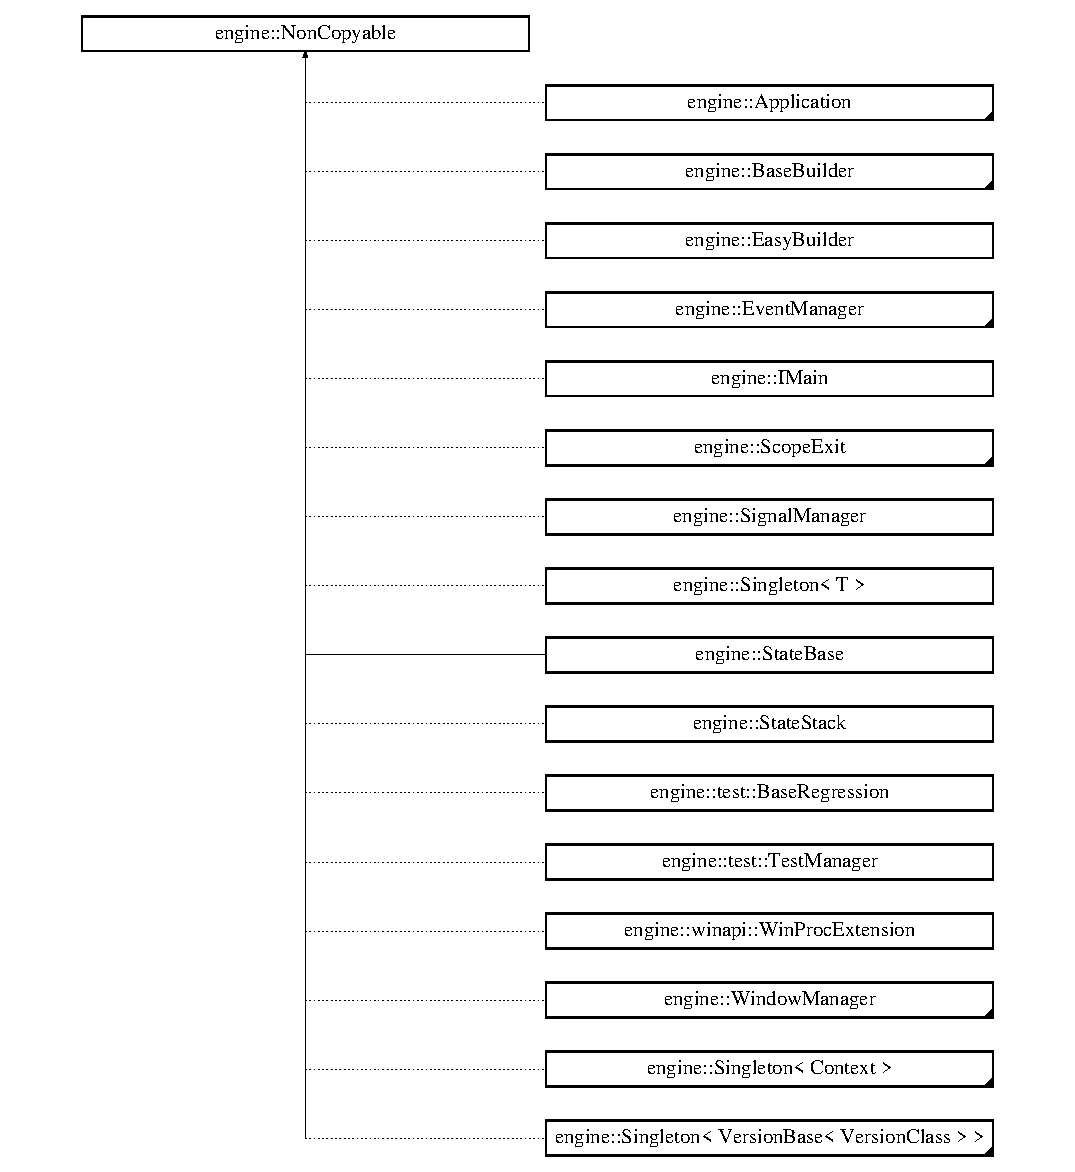
\includegraphics[height=12.000000cm]{a00058}
\end{center}
\end{figure}
\subsubsection*{Public Member Functions}
\begin{DoxyCompactItemize}
\item 
\hyperlink{a00058_a9f7cb34234d5117fbe31e0e82cf164b8}{Non\+Copyable} ()=default
\item 
\hyperlink{a00058_a30addd3c42fbbe053a7484ed209ef8c3}{$\sim$\+Non\+Copyable} ()
\item 
\hyperlink{a00058_a6018f0c6b722b97077bfb807f03f0f69}{Non\+Copyable} (const \hyperlink{a00058}{Non\+Copyable} \&)=delete
\item 
\hyperlink{a00058}{Non\+Copyable} \& \hyperlink{a00058_a21f1cc26f8f967d5c636e580cc728821}{operator=} (const \hyperlink{a00058}{Non\+Copyable} \&)=delete
\end{DoxyCompactItemize}


\subsubsection{Detailed Description}
All classes derived from this class are not copiable. \begin{DoxyWarning}{Warning}
Only private inharitance allowed. 
\end{DoxyWarning}


Definition at line 10 of file Non\+Copyable.\+h.



\subsubsection{Constructor \& Destructor Documentation}
\index{engine\+::\+Non\+Copyable@{engine\+::\+Non\+Copyable}!Non\+Copyable@{Non\+Copyable}}
\index{Non\+Copyable@{Non\+Copyable}!engine\+::\+Non\+Copyable@{engine\+::\+Non\+Copyable}}
\paragraph[{\texorpdfstring{Non\+Copyable()=default}{NonCopyable()=default}}]{\setlength{\rightskip}{0pt plus 5cm}engine\+::\+Non\+Copyable\+::\+Non\+Copyable (
\begin{DoxyParamCaption}
{}
\end{DoxyParamCaption}
)\hspace{0.3cm}{\ttfamily [default]}}\hypertarget{a00058_a9f7cb34234d5117fbe31e0e82cf164b8}{}\label{a00058_a9f7cb34234d5117fbe31e0e82cf164b8}
Default constructable from child classes 

Referenced by $\sim$\+Non\+Copyable().

\index{engine\+::\+Non\+Copyable@{engine\+::\+Non\+Copyable}!````~Non\+Copyable@{$\sim$\+Non\+Copyable}}
\index{````~Non\+Copyable@{$\sim$\+Non\+Copyable}!engine\+::\+Non\+Copyable@{engine\+::\+Non\+Copyable}}
\paragraph[{\texorpdfstring{$\sim$\+Non\+Copyable()}{~NonCopyable()}}]{\setlength{\rightskip}{0pt plus 5cm}engine\+::\+Non\+Copyable\+::$\sim$\+Non\+Copyable (
\begin{DoxyParamCaption}
{}
\end{DoxyParamCaption}
)\hspace{0.3cm}{\ttfamily [inline]}}\hypertarget{a00058_a30addd3c42fbbe053a7484ed209ef8c3}{}\label{a00058_a30addd3c42fbbe053a7484ed209ef8c3}
Non virtual destructor. 

Definition at line 16 of file Non\+Copyable.\+h.

\index{engine\+::\+Non\+Copyable@{engine\+::\+Non\+Copyable}!Non\+Copyable@{Non\+Copyable}}
\index{Non\+Copyable@{Non\+Copyable}!engine\+::\+Non\+Copyable@{engine\+::\+Non\+Copyable}}
\paragraph[{\texorpdfstring{Non\+Copyable(const Non\+Copyable \&)=delete}{NonCopyable(const NonCopyable &)=delete}}]{\setlength{\rightskip}{0pt plus 5cm}engine\+::\+Non\+Copyable\+::\+Non\+Copyable (
\begin{DoxyParamCaption}
\item[{const {\bf Non\+Copyable} \&}]{}
\end{DoxyParamCaption}
)\hspace{0.3cm}{\ttfamily [delete]}}\hypertarget{a00058_a6018f0c6b722b97077bfb807f03f0f69}{}\label{a00058_a6018f0c6b722b97077bfb807f03f0f69}
forbid copy constructor 

\subsubsection{Member Function Documentation}
\index{engine\+::\+Non\+Copyable@{engine\+::\+Non\+Copyable}!operator=@{operator=}}
\index{operator=@{operator=}!engine\+::\+Non\+Copyable@{engine\+::\+Non\+Copyable}}
\paragraph[{\texorpdfstring{operator=(const Non\+Copyable \&)=delete}{operator=(const NonCopyable &)=delete}}]{\setlength{\rightskip}{0pt plus 5cm}{\bf Non\+Copyable}\& engine\+::\+Non\+Copyable\+::operator= (
\begin{DoxyParamCaption}
\item[{const {\bf Non\+Copyable} \&}]{}
\end{DoxyParamCaption}
)\hspace{0.3cm}{\ttfamily [delete]}}\hypertarget{a00058_a21f1cc26f8f967d5c636e580cc728821}{}\label{a00058_a21f1cc26f8f967d5c636e580cc728821}
forbid copy assignment 

Referenced by $\sim$\+Non\+Copyable().



The documentation for this struct was generated from the following file\+:\begin{DoxyCompactItemize}
\item 
E\+:/\+Programing/\+Projects/\+Engine\+Workspace/\+Common\+Libs/engine/include/engine/constraints/Non\+Copyable.\+h\end{DoxyCompactItemize}

\hypertarget{a00059}{}\subsection{engine\+:\+:Non\+Moveable Struct Reference}
\label{a00059}\index{engine\+::\+Non\+Moveable@{engine\+::\+Non\+Moveable}}


{\ttfamily \#include $<$E\+:/\+Programing/\+Projects/\+Engine\+Workspace/\+Common\+Libs/engine/include/engine/constraints/\+Non\+Moveable.\+h$>$}

Inheritance diagram for engine\+:\+:Non\+Moveable\+:\begin{figure}[H]
\begin{center}
\leavevmode
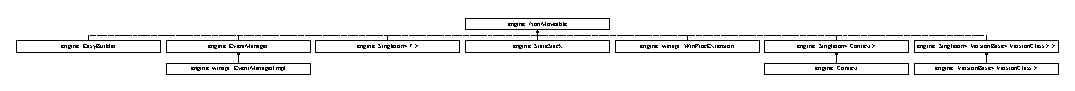
\includegraphics[height=0.771704cm]{a00059}
\end{center}
\end{figure}
\subsubsection*{Public Member Functions}
\begin{DoxyCompactItemize}
\item 
\hyperlink{a00059_afc10190e7b658e00593b253c0d49cb35}{Non\+Moveable} ()=default
\item 
\hyperlink{a00059_a32b7d1f14280ffa724bd6404801a6bef}{Non\+Moveable} (\hyperlink{a00059}{Non\+Moveable} \&\&)=delete
\item 
\hyperlink{a00059}{Non\+Moveable} \& \hyperlink{a00059_ae233a63d597305bc8a2175eab7e498d8}{operator=} (\hyperlink{a00059}{Non\+Moveable} \&\&)=delete
\end{DoxyCompactItemize}


\subsubsection{Detailed Description}
All classes derived from this class are not moveable. \begin{DoxyWarning}{Warning}
Only private inheritance allowed. 
\end{DoxyWarning}


Definition at line 10 of file Non\+Moveable.\+h.



\subsubsection{Constructor \& Destructor Documentation}
\index{engine\+::\+Non\+Moveable@{engine\+::\+Non\+Moveable}!Non\+Moveable@{Non\+Moveable}}
\index{Non\+Moveable@{Non\+Moveable}!engine\+::\+Non\+Moveable@{engine\+::\+Non\+Moveable}}
\paragraph[{\texorpdfstring{Non\+Moveable()=default}{NonMoveable()=default}}]{\setlength{\rightskip}{0pt plus 5cm}engine\+::\+Non\+Moveable\+::\+Non\+Moveable (
\begin{DoxyParamCaption}
{}
\end{DoxyParamCaption}
)\hspace{0.3cm}{\ttfamily [default]}}\hypertarget{a00059_afc10190e7b658e00593b253c0d49cb35}{}\label{a00059_afc10190e7b658e00593b253c0d49cb35}
Default constructable from child classes \index{engine\+::\+Non\+Moveable@{engine\+::\+Non\+Moveable}!Non\+Moveable@{Non\+Moveable}}
\index{Non\+Moveable@{Non\+Moveable}!engine\+::\+Non\+Moveable@{engine\+::\+Non\+Moveable}}
\paragraph[{\texorpdfstring{Non\+Moveable(\+Non\+Moveable \&\&)=delete}{NonMoveable(NonMoveable &&)=delete}}]{\setlength{\rightskip}{0pt plus 5cm}engine\+::\+Non\+Moveable\+::\+Non\+Moveable (
\begin{DoxyParamCaption}
\item[{{\bf Non\+Moveable} \&\&}]{}
\end{DoxyParamCaption}
)\hspace{0.3cm}{\ttfamily [delete]}}\hypertarget{a00059_a32b7d1f14280ffa724bd6404801a6bef}{}\label{a00059_a32b7d1f14280ffa724bd6404801a6bef}
forbid move constructor 

\subsubsection{Member Function Documentation}
\index{engine\+::\+Non\+Moveable@{engine\+::\+Non\+Moveable}!operator=@{operator=}}
\index{operator=@{operator=}!engine\+::\+Non\+Moveable@{engine\+::\+Non\+Moveable}}
\paragraph[{\texorpdfstring{operator=(\+Non\+Moveable \&\&)=delete}{operator=(NonMoveable &&)=delete}}]{\setlength{\rightskip}{0pt plus 5cm}{\bf Non\+Moveable}\& engine\+::\+Non\+Moveable\+::operator= (
\begin{DoxyParamCaption}
\item[{{\bf Non\+Moveable} \&\&}]{}
\end{DoxyParamCaption}
)\hspace{0.3cm}{\ttfamily [delete]}}\hypertarget{a00059_ae233a63d597305bc8a2175eab7e498d8}{}\label{a00059_ae233a63d597305bc8a2175eab7e498d8}
forbid move assignment 

The documentation for this struct was generated from the following file\+:\begin{DoxyCompactItemize}
\item 
E\+:/\+Programing/\+Projects/\+Engine\+Workspace/\+Common\+Libs/engine/include/engine/constraints/Non\+Moveable.\+h\end{DoxyCompactItemize}

\hypertarget{a00060}{}\subsection{engine\+:\+:P\+I\+M\+P\+L\+Copyable$<$ T $>$ Struct Template Reference}
\label{a00060}\index{engine\+::\+P\+I\+M\+P\+L\+Copyable$<$ T $>$@{engine\+::\+P\+I\+M\+P\+L\+Copyable$<$ T $>$}}
\subsubsection*{Public Member Functions}
\begin{DoxyCompactItemize}
\item 
{\bfseries P\+I\+M\+P\+L\+Copyable} (const \hyperlink{a00060}{P\+I\+M\+P\+L\+Copyable} \&o)\hypertarget{a00060_af0ce03b894589b5bd951cc25a073dc65}{}\label{a00060_af0ce03b894589b5bd951cc25a073dc65}

\item 
T \& {\bfseries P\+I\+M\+P\+L\+Copyable\+::operator=} (const \hyperlink{a00060}{P\+I\+M\+P\+L\+Copyable} \&o)\hypertarget{a00060_a26fdb9b3d449d04dc653c7ae942f452b}{}\label{a00060_a26fdb9b3d449d04dc653c7ae942f452b}

\end{DoxyCompactItemize}


\subsubsection{Detailed Description}
\subsubsection*{template$<$class T$>$\\*
struct engine\+::\+P\+I\+M\+P\+L\+Copyable$<$ T $>$}



Definition at line 6 of file P\+I\+M\+P\+L\+Copyable.\+h.



The documentation for this struct was generated from the following file\+:\begin{DoxyCompactItemize}
\item 
E\+:/\+Programing/\+Projects/\+Engine\+Workspace/\+Common\+Libs/engine/include/engine/constraints/P\+I\+M\+P\+L\+Copyable.\+h\end{DoxyCompactItemize}

\hypertarget{a00061}{}\subsection{engine\+:\+:P\+I\+M\+P\+L\+Moveable$<$ T $>$ Struct Template Reference}
\label{a00061}\index{engine\+::\+P\+I\+M\+P\+L\+Moveable$<$ T $>$@{engine\+::\+P\+I\+M\+P\+L\+Moveable$<$ T $>$}}
\subsubsection*{Public Member Functions}
\begin{DoxyCompactItemize}
\item 
{\bfseries P\+I\+M\+P\+L\+Moveable} (\hyperlink{a00061}{P\+I\+M\+P\+L\+Moveable} \&\&o)\hypertarget{a00061_ad0b013508a9b2d94bc084819348bd8a0}{}\label{a00061_ad0b013508a9b2d94bc084819348bd8a0}

\item 
T \& {\bfseries P\+I\+M\+P\+L\+Moveable\+::operator=} (\hyperlink{a00061}{P\+I\+M\+P\+L\+Moveable} \&\&o)\hypertarget{a00061_ac67025e8a25edffe99fa9bf67ed8ca19}{}\label{a00061_ac67025e8a25edffe99fa9bf67ed8ca19}

\end{DoxyCompactItemize}


\subsubsection{Detailed Description}
\subsubsection*{template$<$class T$>$\\*
struct engine\+::\+P\+I\+M\+P\+L\+Moveable$<$ T $>$}



Definition at line 6 of file P\+I\+M\+P\+L\+Moveable.\+h.



The documentation for this struct was generated from the following file\+:\begin{DoxyCompactItemize}
\item 
E\+:/\+Programing/\+Projects/\+Engine\+Workspace/\+Common\+Libs/engine/include/engine/constraints/P\+I\+M\+P\+L\+Moveable.\+h\end{DoxyCompactItemize}

\hypertarget{a00062}{}\subsection{engine\+:\+:Pointer\+Equal\+To$<$ T $>$ Struct Template Reference}
\label{a00062}\index{engine\+::\+Pointer\+Equal\+To$<$ T $>$@{engine\+::\+Pointer\+Equal\+To$<$ T $>$}}


{\ttfamily \#include $<$E\+:/\+Programing/\+Projects/\+Engine\+Workspace/\+Common\+Libs/engine/include/engine/functional/functions.\+h$>$}

\subsubsection*{Public Types}
\begin{DoxyCompactItemize}
\item 
using \hyperlink{a00062_af485b6182246602f97c4f0bef182f799}{Value\+Type} = typename std\+::remove\+\_\+pointer$<$ T $>$\+::type
\item 
using \hyperlink{a00062_accdf0f2f7684859c103e277bc745f869}{Raw\+Pointer\+Type} = \hyperlink{a00062_af485b6182246602f97c4f0bef182f799}{Value\+Type} $\ast$
\item 
using \hyperlink{a00062_ad16a216e6217ae2f08c95f03fdd245cc}{Unique\+Pointer\+Type} = std\+::unique\+\_\+ptr$<$ \hyperlink{a00062_af485b6182246602f97c4f0bef182f799}{Value\+Type} $>$
\item 
using \hyperlink{a00062_a30718c9509a5f19766f8d867ddd08011}{Shared\+Pointer\+Type} = std\+::shared\+\_\+ptr$<$ \hyperlink{a00062_af485b6182246602f97c4f0bef182f799}{Value\+Type} $>$
\item 
using \hyperlink{a00062_ac6a2979606d67d0c973d3f73e7730651}{Weak\+Pointer\+Type} = std\+::weak\+\_\+ptr$<$ \hyperlink{a00062_af485b6182246602f97c4f0bef182f799}{Value\+Type} $>$
\end{DoxyCompactItemize}
\subsubsection*{Public Member Functions}
\begin{DoxyCompactItemize}
\item 
\hyperlink{a00062_a25356ec570fd1f0c1395c2ea7dcdc839}{Pointer\+Equal\+To} (const \hyperlink{a00062_accdf0f2f7684859c103e277bc745f869}{Raw\+Pointer\+Type} \&v)
\item 
bool \hyperlink{a00062_aa95f53dfe2393421d25b5bf6f458cb53}{operator()} (const \hyperlink{a00062_accdf0f2f7684859c103e277bc745f869}{Raw\+Pointer\+Type} \&o)
\item 
bool \hyperlink{a00062_abc68beffa9e32f7dd0caff6ce3d36e84}{operator()} (const \hyperlink{a00062_ad16a216e6217ae2f08c95f03fdd245cc}{Unique\+Pointer\+Type} \&o)
\item 
bool \hyperlink{a00062_a5183273e9ba9a58234466b34adac373c}{operator()} (const \hyperlink{a00062_a30718c9509a5f19766f8d867ddd08011}{Shared\+Pointer\+Type} \&o)
\item 
bool \hyperlink{a00062_acdb87526d0e9c0aa8d235bf2e6cc5e97}{operator()} (const \hyperlink{a00062_ac6a2979606d67d0c973d3f73e7730651}{Weak\+Pointer\+Type} \&o)
\end{DoxyCompactItemize}


\subsubsection{Detailed Description}
\subsubsection*{template$<$typename T$>$\\*
struct engine\+::\+Pointer\+Equal\+To$<$ T $>$}

Functional for equality check in standard algorithms for different pointer types. 

Definition at line 34 of file functions.\+h.



\subsubsection{Member Typedef Documentation}
\index{engine\+::\+Pointer\+Equal\+To@{engine\+::\+Pointer\+Equal\+To}!Raw\+Pointer\+Type@{Raw\+Pointer\+Type}}
\index{Raw\+Pointer\+Type@{Raw\+Pointer\+Type}!engine\+::\+Pointer\+Equal\+To@{engine\+::\+Pointer\+Equal\+To}}
\paragraph[{\texorpdfstring{Raw\+Pointer\+Type}{RawPointerType}}]{\setlength{\rightskip}{0pt plus 5cm}template$<$typename T $>$ using {\bf engine\+::\+Pointer\+Equal\+To}$<$ T $>$\+::{\bf Raw\+Pointer\+Type} =  {\bf Value\+Type}$\ast$}\hypertarget{a00062_accdf0f2f7684859c103e277bc745f869}{}\label{a00062_accdf0f2f7684859c103e277bc745f869}
Raw pointer type 

Definition at line 39 of file functions.\+h.

\index{engine\+::\+Pointer\+Equal\+To@{engine\+::\+Pointer\+Equal\+To}!Shared\+Pointer\+Type@{Shared\+Pointer\+Type}}
\index{Shared\+Pointer\+Type@{Shared\+Pointer\+Type}!engine\+::\+Pointer\+Equal\+To@{engine\+::\+Pointer\+Equal\+To}}
\paragraph[{\texorpdfstring{Shared\+Pointer\+Type}{SharedPointerType}}]{\setlength{\rightskip}{0pt plus 5cm}template$<$typename T $>$ using {\bf engine\+::\+Pointer\+Equal\+To}$<$ T $>$\+::{\bf Shared\+Pointer\+Type} =  std\+::shared\+\_\+ptr $<$ {\bf Value\+Type} $>$}\hypertarget{a00062_a30718c9509a5f19766f8d867ddd08011}{}\label{a00062_a30718c9509a5f19766f8d867ddd08011}
Shared pointer type 

Definition at line 43 of file functions.\+h.

\index{engine\+::\+Pointer\+Equal\+To@{engine\+::\+Pointer\+Equal\+To}!Unique\+Pointer\+Type@{Unique\+Pointer\+Type}}
\index{Unique\+Pointer\+Type@{Unique\+Pointer\+Type}!engine\+::\+Pointer\+Equal\+To@{engine\+::\+Pointer\+Equal\+To}}
\paragraph[{\texorpdfstring{Unique\+Pointer\+Type}{UniquePointerType}}]{\setlength{\rightskip}{0pt plus 5cm}template$<$typename T $>$ using {\bf engine\+::\+Pointer\+Equal\+To}$<$ T $>$\+::{\bf Unique\+Pointer\+Type} =  std\+::unique\+\_\+ptr $<$ {\bf Value\+Type} $>$}\hypertarget{a00062_ad16a216e6217ae2f08c95f03fdd245cc}{}\label{a00062_ad16a216e6217ae2f08c95f03fdd245cc}
Unique pointer type 

Definition at line 41 of file functions.\+h.

\index{engine\+::\+Pointer\+Equal\+To@{engine\+::\+Pointer\+Equal\+To}!Value\+Type@{Value\+Type}}
\index{Value\+Type@{Value\+Type}!engine\+::\+Pointer\+Equal\+To@{engine\+::\+Pointer\+Equal\+To}}
\paragraph[{\texorpdfstring{Value\+Type}{ValueType}}]{\setlength{\rightskip}{0pt plus 5cm}template$<$typename T $>$ using {\bf engine\+::\+Pointer\+Equal\+To}$<$ T $>$\+::{\bf Value\+Type} =  typename std\+::remove\+\_\+pointer$<$T$>$\+::type}\hypertarget{a00062_af485b6182246602f97c4f0bef182f799}{}\label{a00062_af485b6182246602f97c4f0bef182f799}
Type without pointer 

Definition at line 37 of file functions.\+h.

\index{engine\+::\+Pointer\+Equal\+To@{engine\+::\+Pointer\+Equal\+To}!Weak\+Pointer\+Type@{Weak\+Pointer\+Type}}
\index{Weak\+Pointer\+Type@{Weak\+Pointer\+Type}!engine\+::\+Pointer\+Equal\+To@{engine\+::\+Pointer\+Equal\+To}}
\paragraph[{\texorpdfstring{Weak\+Pointer\+Type}{WeakPointerType}}]{\setlength{\rightskip}{0pt plus 5cm}template$<$typename T $>$ using {\bf engine\+::\+Pointer\+Equal\+To}$<$ T $>$\+::{\bf Weak\+Pointer\+Type} =  std\+::weak\+\_\+ptr $<$ {\bf Value\+Type} $>$}\hypertarget{a00062_ac6a2979606d67d0c973d3f73e7730651}{}\label{a00062_ac6a2979606d67d0c973d3f73e7730651}
Weak pointer type 

Definition at line 45 of file functions.\+h.



\subsubsection{Constructor \& Destructor Documentation}
\index{engine\+::\+Pointer\+Equal\+To@{engine\+::\+Pointer\+Equal\+To}!Pointer\+Equal\+To@{Pointer\+Equal\+To}}
\index{Pointer\+Equal\+To@{Pointer\+Equal\+To}!engine\+::\+Pointer\+Equal\+To@{engine\+::\+Pointer\+Equal\+To}}
\paragraph[{\texorpdfstring{Pointer\+Equal\+To(const Raw\+Pointer\+Type \&v)}{PointerEqualTo(const RawPointerType &v)}}]{\setlength{\rightskip}{0pt plus 5cm}template$<$typename T $>$ {\bf engine\+::\+Pointer\+Equal\+To}$<$ T $>$\+::{\bf Pointer\+Equal\+To} (
\begin{DoxyParamCaption}
\item[{const {\bf Raw\+Pointer\+Type} \&}]{v}
\end{DoxyParamCaption}
)\hspace{0.3cm}{\ttfamily [inline]}}\hypertarget{a00062_a25356ec570fd1f0c1395c2ea7dcdc839}{}\label{a00062_a25356ec570fd1f0c1395c2ea7dcdc839}
Construct the equality check 
\begin{DoxyParams}{Parameters}
{\em v} & pointer to check \\
\hline
\end{DoxyParams}


Definition at line 51 of file functions.\+h.



\subsubsection{Member Function Documentation}
\index{engine\+::\+Pointer\+Equal\+To@{engine\+::\+Pointer\+Equal\+To}!operator()@{operator()}}
\index{operator()@{operator()}!engine\+::\+Pointer\+Equal\+To@{engine\+::\+Pointer\+Equal\+To}}
\paragraph[{\texorpdfstring{operator()(const Raw\+Pointer\+Type \&o)}{operator()(const RawPointerType &o)}}]{\setlength{\rightskip}{0pt plus 5cm}template$<$typename T $>$ bool {\bf engine\+::\+Pointer\+Equal\+To}$<$ T $>$\+::operator() (
\begin{DoxyParamCaption}
\item[{const {\bf Raw\+Pointer\+Type} \&}]{o}
\end{DoxyParamCaption}
)\hspace{0.3cm}{\ttfamily [inline]}}\hypertarget{a00062_aa95f53dfe2393421d25b5bf6f458cb53}{}\label{a00062_aa95f53dfe2393421d25b5bf6f458cb53}
Check whether the given object equals to our one. 
\begin{DoxyParams}{Parameters}
{\em o} & object to check whether equals to the stored value. \\
\hline
\end{DoxyParams}
\begin{DoxyReturn}{Returns}
Returns true if the given object equals to the stored one. 
\end{DoxyReturn}


Definition at line 60 of file functions.\+h.



Referenced by engine\+::\+Pointer\+Equal\+To$<$ T $>$\+::operator()().

\index{engine\+::\+Pointer\+Equal\+To@{engine\+::\+Pointer\+Equal\+To}!operator()@{operator()}}
\index{operator()@{operator()}!engine\+::\+Pointer\+Equal\+To@{engine\+::\+Pointer\+Equal\+To}}
\paragraph[{\texorpdfstring{operator()(const Unique\+Pointer\+Type \&o)}{operator()(const UniquePointerType &o)}}]{\setlength{\rightskip}{0pt plus 5cm}template$<$typename T $>$ bool {\bf engine\+::\+Pointer\+Equal\+To}$<$ T $>$\+::operator() (
\begin{DoxyParamCaption}
\item[{const {\bf Unique\+Pointer\+Type} \&}]{o}
\end{DoxyParamCaption}
)\hspace{0.3cm}{\ttfamily [inline]}}\hypertarget{a00062_abc68beffa9e32f7dd0caff6ce3d36e84}{}\label{a00062_abc68beffa9e32f7dd0caff6ce3d36e84}
Check whether the given object equals to our one. 
\begin{DoxyParams}{Parameters}
{\em o} & object to check whether equals to the stored value. \\
\hline
\end{DoxyParams}
\begin{DoxyReturn}{Returns}
Returns true if the given object equals to the stored one. 
\end{DoxyReturn}


Definition at line 66 of file functions.\+h.

\index{engine\+::\+Pointer\+Equal\+To@{engine\+::\+Pointer\+Equal\+To}!operator()@{operator()}}
\index{operator()@{operator()}!engine\+::\+Pointer\+Equal\+To@{engine\+::\+Pointer\+Equal\+To}}
\paragraph[{\texorpdfstring{operator()(const Shared\+Pointer\+Type \&o)}{operator()(const SharedPointerType &o)}}]{\setlength{\rightskip}{0pt plus 5cm}template$<$typename T $>$ bool {\bf engine\+::\+Pointer\+Equal\+To}$<$ T $>$\+::operator() (
\begin{DoxyParamCaption}
\item[{const {\bf Shared\+Pointer\+Type} \&}]{o}
\end{DoxyParamCaption}
)\hspace{0.3cm}{\ttfamily [inline]}}\hypertarget{a00062_a5183273e9ba9a58234466b34adac373c}{}\label{a00062_a5183273e9ba9a58234466b34adac373c}
Check whether the given object equals to our one. 
\begin{DoxyParams}{Parameters}
{\em o} & object to check whether equals to the stored value. \\
\hline
\end{DoxyParams}
\begin{DoxyReturn}{Returns}
Returns true if the given object equals to the stored one. 
\end{DoxyReturn}


Definition at line 72 of file functions.\+h.

\index{engine\+::\+Pointer\+Equal\+To@{engine\+::\+Pointer\+Equal\+To}!operator()@{operator()}}
\index{operator()@{operator()}!engine\+::\+Pointer\+Equal\+To@{engine\+::\+Pointer\+Equal\+To}}
\paragraph[{\texorpdfstring{operator()(const Weak\+Pointer\+Type \&o)}{operator()(const WeakPointerType &o)}}]{\setlength{\rightskip}{0pt plus 5cm}template$<$typename T $>$ bool {\bf engine\+::\+Pointer\+Equal\+To}$<$ T $>$\+::operator() (
\begin{DoxyParamCaption}
\item[{const {\bf Weak\+Pointer\+Type} \&}]{o}
\end{DoxyParamCaption}
)\hspace{0.3cm}{\ttfamily [inline]}}\hypertarget{a00062_acdb87526d0e9c0aa8d235bf2e6cc5e97}{}\label{a00062_acdb87526d0e9c0aa8d235bf2e6cc5e97}
Check whether the given object equals to our one. 
\begin{DoxyParams}{Parameters}
{\em o} & object to check whether equals to the stored value. \\
\hline
\end{DoxyParams}
\begin{DoxyReturn}{Returns}
Returns true if the given object equals to the stored one. 
\end{DoxyReturn}


Definition at line 78 of file functions.\+h.



The documentation for this struct was generated from the following file\+:\begin{DoxyCompactItemize}
\item 
E\+:/\+Programing/\+Projects/\+Engine\+Workspace/\+Common\+Libs/engine/include/engine/functional/functions.\+h\end{DoxyCompactItemize}

\hypertarget{a00063}{}\subsection{engine\+:\+:Scope\+Exit Class Reference}
\label{a00063}\index{engine\+::\+Scope\+Exit@{engine\+::\+Scope\+Exit}}
Inheritance diagram for engine\+:\+:Scope\+Exit\+:\begin{figure}[H]
\begin{center}
\leavevmode
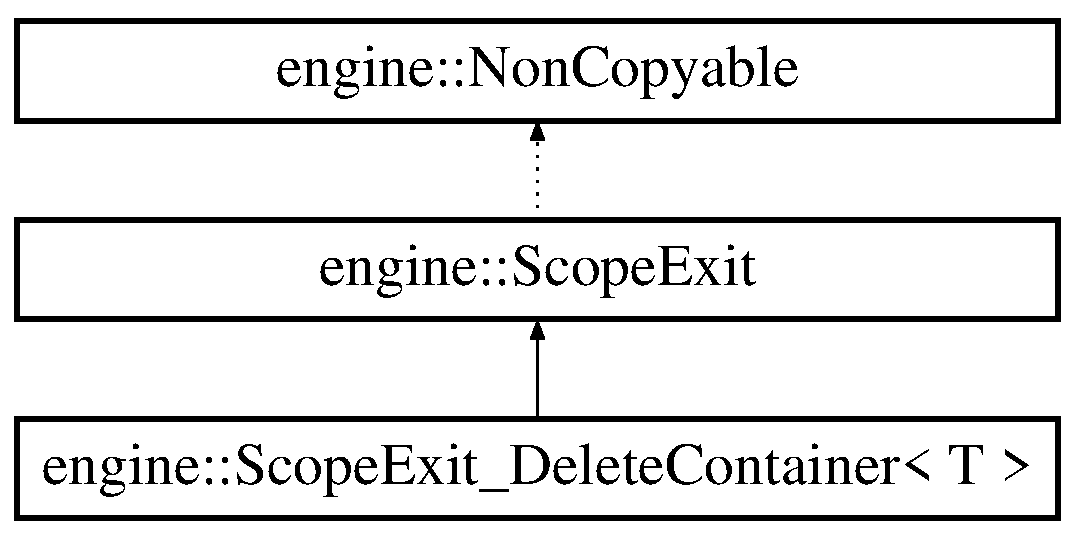
\includegraphics[height=3.000000cm]{a00063}
\end{center}
\end{figure}
\subsubsection*{Public Member Functions}
\begin{DoxyCompactItemize}
\item 
{\bfseries Scope\+Exit} (std\+::function$<$ void()$>$ \&\&f)\hypertarget{a00063_a6003e466fdda9061f2916b7e13265047}{}\label{a00063_a6003e466fdda9061f2916b7e13265047}

\item 
{\bfseries Scope\+Exit} (\hyperlink{a00063}{Scope\+Exit} \&\&o)\hypertarget{a00063_ad4bcbbc60dd9951caadca85b22688efb}{}\label{a00063_ad4bcbbc60dd9951caadca85b22688efb}

\item 
\hyperlink{a00063}{Scope\+Exit} \& {\bfseries operator=} (\hyperlink{a00063}{Scope\+Exit} \&\&o)\hypertarget{a00063_aa03378e947cf4ed0d2802d37384a35a4}{}\label{a00063_aa03378e947cf4ed0d2802d37384a35a4}

\end{DoxyCompactItemize}


\subsubsection{Detailed Description}


Definition at line 7 of file Scope\+Exit.\+h.



The documentation for this class was generated from the following file\+:\begin{DoxyCompactItemize}
\item 
E\+:/\+Programing/\+Projects/\+Engine\+Workspace/\+Common\+Libs/engine/include/engine/utils/Scope\+Exit.\+h\end{DoxyCompactItemize}

\hypertarget{a00064}{}\subsection{engine\+:\+:Scope\+Exit\+\_\+\+Delete\+Container$<$ T $>$ Struct Template Reference}
\label{a00064}\index{engine\+::\+Scope\+Exit\+\_\+\+Delete\+Container$<$ T $>$@{engine\+::\+Scope\+Exit\+\_\+\+Delete\+Container$<$ T $>$}}
Inheritance diagram for engine\+:\+:Scope\+Exit\+\_\+\+Delete\+Container$<$ T $>$\+:\begin{figure}[H]
\begin{center}
\leavevmode
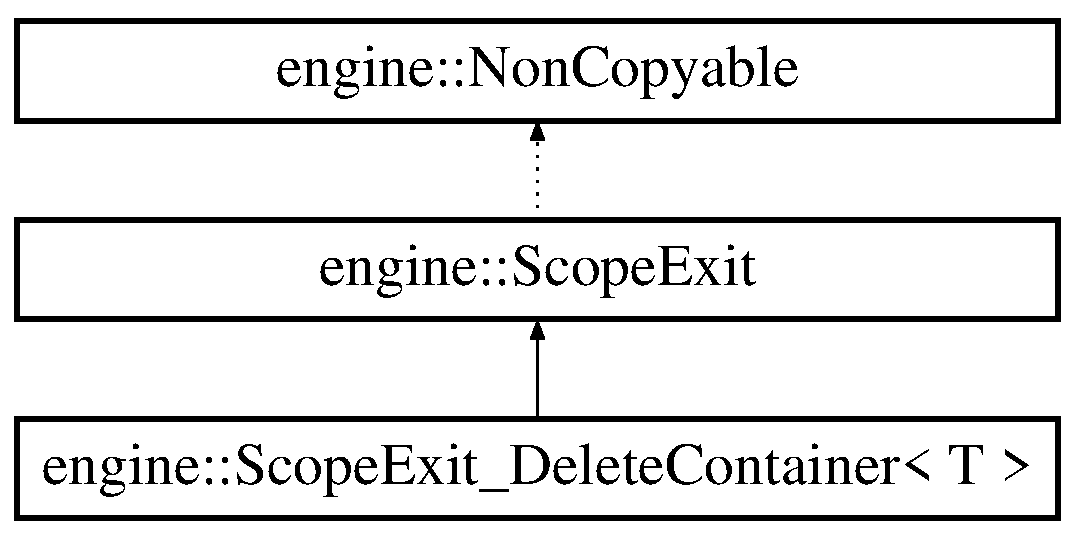
\includegraphics[height=3.000000cm]{a00064}
\end{center}
\end{figure}
\subsubsection*{Public Member Functions}
\begin{DoxyCompactItemize}
\item 
{\bfseries Scope\+Exit\+\_\+\+Delete\+Container} (T \&container)\hypertarget{a00064_a2f092ad5ade85806194ba49e4431ac10}{}\label{a00064_a2f092ad5ade85806194ba49e4431ac10}

\end{DoxyCompactItemize}
\subsubsection*{Static Public Member Functions}
\begin{DoxyCompactItemize}
\item 
static void {\bfseries delete\+Container} (T \&container)\hypertarget{a00064_aee150e0726f1f78446279420a52e13c0}{}\label{a00064_aee150e0726f1f78446279420a52e13c0}

\end{DoxyCompactItemize}


\subsubsection{Detailed Description}
\subsubsection*{template$<$class T$>$\\*
struct engine\+::\+Scope\+Exit\+\_\+\+Delete\+Container$<$ T $>$}



Definition at line 33 of file Scope\+Exit.\+h.



The documentation for this struct was generated from the following file\+:\begin{DoxyCompactItemize}
\item 
E\+:/\+Programing/\+Projects/\+Engine\+Workspace/\+Common\+Libs/engine/include/engine/utils/Scope\+Exit.\+h\end{DoxyCompactItemize}

\hypertarget{a00065}{}\subsection{engine\+:\+:Signal$<$ Args $>$ Class Template Reference}
\label{a00065}\index{engine\+::\+Signal$<$ Args $>$@{engine\+::\+Signal$<$ Args $>$}}


{\ttfamily \#include $<$E\+:/\+Programing/\+Projects/\+Engine\+Workspace/\+Common\+Libs/engine/include/engine/signal\+Slot/\+Signal.\+h$>$}

Inheritance diagram for engine\+:\+:Signal$<$ Args $>$\+:\begin{figure}[H]
\begin{center}
\leavevmode
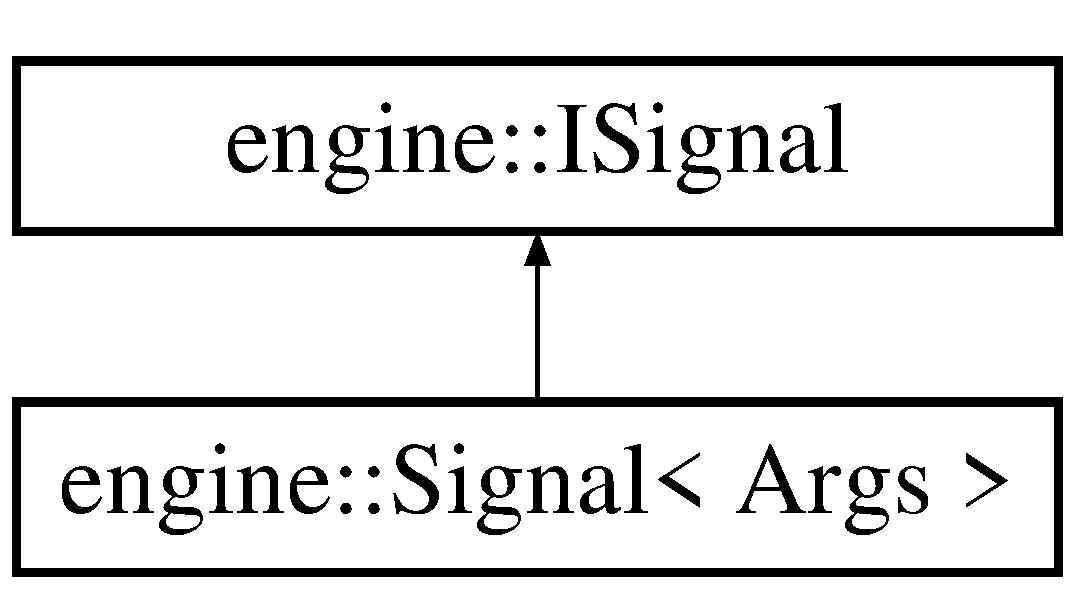
\includegraphics[height=2.000000cm]{a00065}
\end{center}
\end{figure}
\subsubsection*{Public Member Functions}
\begin{DoxyCompactItemize}
\item 
\hyperlink{a00065_ac27bc541be14d6ad516d858c3039df97}{Signal} ()=default
\item 
\hyperlink{a00065_a29c5d469f7f68d00e6895d1cf5121025}{$\sim$\+Signal} () override
\item 
{\footnotesize template$<$class T , void(\+T\+::$\ast$)(\+Args...) slot$>$ }\\void \hyperlink{a00065_aba0c679c2026a6ddaafdac1f6a71cb70}{connect} (T $\ast$holder)
\item 
{\footnotesize template$<$class T , void(\+T\+::$\ast$)(\+Args...) slot$>$ }\\void \hyperlink{a00065_a4dc6184edbd36dd8717d07c37a1f5fad}{disconnect} (T $\ast$holder)
\item 
{\footnotesize template$<$class T $>$ }\\void \hyperlink{a00065_a4f3a4fcb844c23af742eac03e26bbc1b}{disconnect\+All} (T $\ast$holder)
\item 
void \hyperlink{a00065_afbe3d238443fab207b5030ac8c77385c}{emit} (Args...\+args)
\end{DoxyCompactItemize}


\subsubsection{Detailed Description}
\subsubsection*{template$<$typename... Args$>$\\*
class engine\+::\+Signal$<$ Args $>$}

This class implements a signal. A signal can be emitted in this case all the slots will be called. The call is depend on the slot\textquotesingle{}s signal\+Manager. 
\begin{DoxyTemplParams}{Template Parameters}
{\em Args} & Signature of the signal. \\
\hline
\end{DoxyTemplParams}


Definition at line 20 of file Signal.\+h.



\subsubsection{Constructor \& Destructor Documentation}
\index{engine\+::\+Signal@{engine\+::\+Signal}!Signal@{Signal}}
\index{Signal@{Signal}!engine\+::\+Signal@{engine\+::\+Signal}}
\paragraph[{\texorpdfstring{Signal()=default}{Signal()=default}}]{\setlength{\rightskip}{0pt plus 5cm}template$<$typename... Args$>$ {\bf engine\+::\+Signal}$<$ Args $>$\+::{\bf Signal} (
\begin{DoxyParamCaption}
{}
\end{DoxyParamCaption}
)\hspace{0.3cm}{\ttfamily [default]}}\hypertarget{a00065_ac27bc541be14d6ad516d858c3039df97}{}\label{a00065_ac27bc541be14d6ad516d858c3039df97}
Defualt constructor. \index{engine\+::\+Signal@{engine\+::\+Signal}!````~Signal@{$\sim$\+Signal}}
\index{````~Signal@{$\sim$\+Signal}!engine\+::\+Signal@{engine\+::\+Signal}}
\paragraph[{\texorpdfstring{$\sim$\+Signal() override}{~Signal() override}}]{\setlength{\rightskip}{0pt plus 5cm}template$<$typename... Args$>$ {\bf engine\+::\+Signal}$<$ Args $>$\+::$\sim${\bf Signal} (
\begin{DoxyParamCaption}
{}
\end{DoxyParamCaption}
)\hspace{0.3cm}{\ttfamily [override]}}\hypertarget{a00065_a29c5d469f7f68d00e6895d1cf5121025}{}\label{a00065_a29c5d469f7f68d00e6895d1cf5121025}
Notify all connected slot 

\subsubsection{Member Function Documentation}
\index{engine\+::\+Signal@{engine\+::\+Signal}!connect@{connect}}
\index{connect@{connect}!engine\+::\+Signal@{engine\+::\+Signal}}
\paragraph[{\texorpdfstring{connect(\+T $\ast$holder)}{connect(T *holder)}}]{\setlength{\rightskip}{0pt plus 5cm}template$<$typename... Args$>$ template$<$class T , void(\+T\+::$\ast$)(\+Args...) slot$>$ void {\bf engine\+::\+Signal}$<$ Args $>$\+::connect (
\begin{DoxyParamCaption}
\item[{T $\ast$}]{holder}
\end{DoxyParamCaption}
)}\hypertarget{a00065_aba0c679c2026a6ddaafdac1f6a71cb70}{}\label{a00065_aba0c679c2026a6ddaafdac1f6a71cb70}
Connect the holder member function to this signal. When the signal is emitted a task will crated which will call this member function on the given object. 
\begin{DoxyTemplParams}{Template Parameters}
{\em slot} & Slot to connect to this signal \\
\hline
\end{DoxyTemplParams}

\begin{DoxyParams}{Parameters}
{\em holder} & owner of the slot. \\
\hline
\end{DoxyParams}
\index{engine\+::\+Signal@{engine\+::\+Signal}!disconnect@{disconnect}}
\index{disconnect@{disconnect}!engine\+::\+Signal@{engine\+::\+Signal}}
\paragraph[{\texorpdfstring{disconnect(\+T $\ast$holder)}{disconnect(T *holder)}}]{\setlength{\rightskip}{0pt plus 5cm}template$<$typename... Args$>$ template$<$class T , void(\+T\+::$\ast$)(\+Args...) slot$>$ void {\bf engine\+::\+Signal}$<$ Args $>$\+::disconnect (
\begin{DoxyParamCaption}
\item[{T $\ast$}]{holder}
\end{DoxyParamCaption}
)}\hypertarget{a00065_a4dc6184edbd36dd8717d07c37a1f5fad}{}\label{a00065_a4dc6184edbd36dd8717d07c37a1f5fad}
Disconnect the given slot and object from this signal. Via the shared pointer all the created tasks are invalidated. 
\begin{DoxyTemplParams}{Template Parameters}
{\em slot} & Slot to disconnect to this signal \\
\hline
\end{DoxyTemplParams}

\begin{DoxyParams}{Parameters}
{\em holder} & owner of the slot. \\
\hline
\end{DoxyParams}
\index{engine\+::\+Signal@{engine\+::\+Signal}!disconnect\+All@{disconnect\+All}}
\index{disconnect\+All@{disconnect\+All}!engine\+::\+Signal@{engine\+::\+Signal}}
\paragraph[{\texorpdfstring{disconnect\+All(\+T $\ast$holder)}{disconnectAll(T *holder)}}]{\setlength{\rightskip}{0pt plus 5cm}template$<$typename... Args$>$ template$<$class T $>$ void {\bf engine\+::\+Signal}$<$ Args $>$\+::disconnect\+All (
\begin{DoxyParamCaption}
\item[{T $\ast$}]{holder}
\end{DoxyParamCaption}
)}\hypertarget{a00065_a4f3a4fcb844c23af742eac03e26bbc1b}{}\label{a00065_a4f3a4fcb844c23af742eac03e26bbc1b}
Disconnect all the slots of the given slot holder 
\begin{DoxyParams}{Parameters}
{\em holder} & owner of the slot \\
\hline
\end{DoxyParams}
\index{engine\+::\+Signal@{engine\+::\+Signal}!emit@{emit}}
\index{emit@{emit}!engine\+::\+Signal@{engine\+::\+Signal}}
\paragraph[{\texorpdfstring{emit(\+Args...\+args)}{emit(Args...args)}}]{\setlength{\rightskip}{0pt plus 5cm}template$<$typename... Args$>$ void {\bf engine\+::\+Signal}$<$ Args $>$\+::emit (
\begin{DoxyParamCaption}
\item[{Args...}]{args}
\end{DoxyParamCaption}
)}\hypertarget{a00065_afbe3d238443fab207b5030ac8c77385c}{}\label{a00065_afbe3d238443fab207b5030ac8c77385c}
Emit the signal. For all the connected slot a task is created and added to the corresponding signal manager. 

The documentation for this class was generated from the following file\+:\begin{DoxyCompactItemize}
\item 
E\+:/\+Programing/\+Projects/\+Engine\+Workspace/\+Common\+Libs/engine/include/engine/signal\+Slot/Signal.\+h\end{DoxyCompactItemize}

\hypertarget{a00066}{}\subsection{engine\+:\+:Signal\+Caller$<$ Ts $>$ Class Template Reference}
\label{a00066}\index{engine\+::\+Signal\+Caller$<$ Ts $>$@{engine\+::\+Signal\+Caller$<$ Ts $>$}}


{\ttfamily \#include $<$E\+:/\+Programing/\+Projects/\+Engine\+Workspace/\+Common\+Libs/engine/include/engine/signal\+Slot/\+Signal\+Caller.\+h$>$}

\subsubsection*{Public Member Functions}
\begin{DoxyCompactItemize}
\item 
\hyperlink{a00066_a0ac1c86918e5e9398dbb1cb587835ee1}{Signal\+Caller} (const std\+::function$<$ void(Ts...)$>$ \&func)
\item 
void \hyperlink{a00066_a51aed6d729065df2d78aa8acab3e0eb9}{operator()} (const std\+::tuple$<$ Ts... $>$ \&args)
\end{DoxyCompactItemize}
\subsubsection*{Static Public Member Functions}
\begin{DoxyCompactItemize}
\item 
{\footnotesize template$<$typename T $>$ }\\static std\+::function$<$ void(Ts...)$>$ \hyperlink{a00066_a6a9a7e7fc96f6921fc74b6386651afdc}{create\+Callable} (T $\ast$t, void(T\+::$\ast$callback)(Ts...))
\end{DoxyCompactItemize}


\subsubsection{Detailed Description}
\subsubsection*{template$<$typename... Ts$>$\\*
class engine\+::\+Signal\+Caller$<$ Ts $>$}

This class is responsible for calling a signal\textquotesingle{}s slot on a given object with the stored paramters. 

Definition at line 13 of file Signal\+Caller.\+h.



\subsubsection{Constructor \& Destructor Documentation}
\index{engine\+::\+Signal\+Caller@{engine\+::\+Signal\+Caller}!Signal\+Caller@{Signal\+Caller}}
\index{Signal\+Caller@{Signal\+Caller}!engine\+::\+Signal\+Caller@{engine\+::\+Signal\+Caller}}
\paragraph[{\texorpdfstring{Signal\+Caller(const std\+::function$<$ void(\+Ts...)$>$ \&func)}{SignalCaller(const std::function< void(Ts...)> &func)}}]{\setlength{\rightskip}{0pt plus 5cm}template$<$typename... Ts$>$ {\bf engine\+::\+Signal\+Caller}$<$ Ts $>$\+::{\bf Signal\+Caller} (
\begin{DoxyParamCaption}
\item[{const std\+::function$<$ void(Ts...)$>$ \&}]{func}
\end{DoxyParamCaption}
)\hspace{0.3cm}{\ttfamily [inline]}, {\ttfamily [explicit]}}\hypertarget{a00066_a0ac1c86918e5e9398dbb1cb587835ee1}{}\label{a00066_a0ac1c86918e5e9398dbb1cb587835ee1}
Store the callback function and call it when it is necessery. The function paramter can be produced via static functions \begin{DoxySeeAlso}{See also}
\hyperlink{a00066_a6a9a7e7fc96f6921fc74b6386651afdc}{Signal\+Caller\+::create\+Callable} 
\end{DoxySeeAlso}

\begin{DoxyParams}{Parameters}
{\em func} & Function which will be called with the given parameters \\
\hline
\end{DoxyParams}


Definition at line 52 of file Signal\+Caller.\+h.



\subsubsection{Member Function Documentation}
\index{engine\+::\+Signal\+Caller@{engine\+::\+Signal\+Caller}!create\+Callable@{create\+Callable}}
\index{create\+Callable@{create\+Callable}!engine\+::\+Signal\+Caller@{engine\+::\+Signal\+Caller}}
\paragraph[{\texorpdfstring{create\+Callable(\+T $\ast$t, void(\+T\+::$\ast$callback)(\+Ts...))}{createCallable(T *t, void(T::*callback)(Ts...))}}]{\setlength{\rightskip}{0pt plus 5cm}template$<$typename... Ts$>$ template$<$typename T $>$ static std\+::function$<$void(Ts...)$>$ {\bf engine\+::\+Signal\+Caller}$<$ Ts $>$\+::create\+Callable (
\begin{DoxyParamCaption}
\item[{T $\ast$}]{t, }
\item[{void(T\+::$\ast$)(Ts...)}]{callback}
\end{DoxyParamCaption}
)\hspace{0.3cm}{\ttfamily [inline]}, {\ttfamily [static]}}\hypertarget{a00066_a6a9a7e7fc96f6921fc74b6386651afdc}{}\label{a00066_a6a9a7e7fc96f6921fc74b6386651afdc}
Bind the callback to the given t object. It creates a function which is bind the callback to the t object. 
\begin{DoxyParams}{Parameters}
{\em t} & object which will be assigned to the callback. \\
\hline
{\em callback} & This member function will be called on the t object. \\
\hline
\end{DoxyParams}
\begin{DoxyReturn}{Returns}
Returns a function which will call the member function on the given object. 
\end{DoxyReturn}


Definition at line 24 of file Signal\+Caller.\+h.

\index{engine\+::\+Signal\+Caller@{engine\+::\+Signal\+Caller}!operator()@{operator()}}
\index{operator()@{operator()}!engine\+::\+Signal\+Caller@{engine\+::\+Signal\+Caller}}
\paragraph[{\texorpdfstring{operator()(const std\+::tuple$<$ Ts... $>$ \&args)}{operator()(const std::tuple< Ts... > &args)}}]{\setlength{\rightskip}{0pt plus 5cm}template$<$typename... Ts$>$ void {\bf engine\+::\+Signal\+Caller}$<$ Ts $>$\+::operator() (
\begin{DoxyParamCaption}
\item[{const std\+::tuple$<$ Ts... $>$ \&}]{args}
\end{DoxyParamCaption}
)\hspace{0.3cm}{\ttfamily [inline]}}\hypertarget{a00066_a51aed6d729065df2d78aa8acab3e0eb9}{}\label{a00066_a51aed6d729065df2d78aa8acab3e0eb9}
Calls the stored function with the given parameters. 
\begin{DoxyParams}{Parameters}
{\em args} & Arguments for the stored function. \\
\hline
\end{DoxyParams}


Definition at line 60 of file Signal\+Caller.\+h.



The documentation for this class was generated from the following file\+:\begin{DoxyCompactItemize}
\item 
E\+:/\+Programing/\+Projects/\+Engine\+Workspace/\+Common\+Libs/engine/include/engine/signal\+Slot/Signal\+Caller.\+h\end{DoxyCompactItemize}

\hypertarget{a00067}{}\subsection{engine\+:\+:Signal\+Manager Class Reference}
\label{a00067}\index{engine\+::\+Signal\+Manager@{engine\+::\+Signal\+Manager}}


{\ttfamily \#include $<$E\+:/\+Programing/\+Projects/\+Engine\+Workspace/\+Common\+Libs/engine/include/engine/signal\+Slot/\+Signal\+Manager.\+h$>$}

Inheritance diagram for engine\+:\+:Signal\+Manager\+:\begin{figure}[H]
\begin{center}
\leavevmode
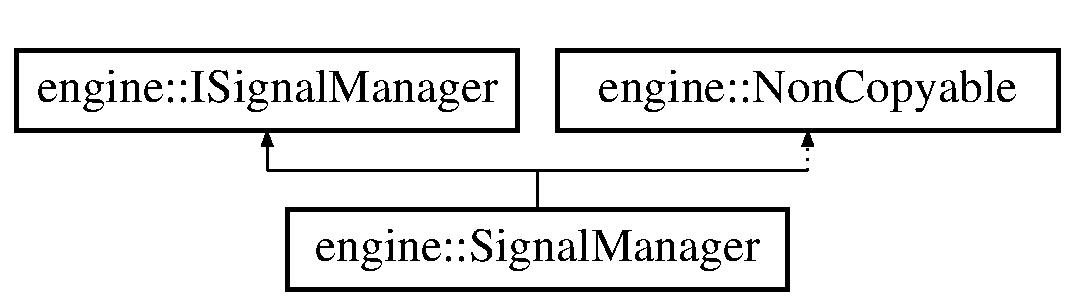
\includegraphics[height=2.000000cm]{a00067}
\end{center}
\end{figure}
\subsubsection*{Public Member Functions}
\begin{DoxyCompactItemize}
\item 
\hyperlink{a00067_aba0cfccea1f10a10e9de9193fb62f358}{Signal\+Manager} ()
\item 
\hyperlink{a00067_a1ad7e4f03ac0657b1ecf90c981053cde}{$\sim$\+Signal\+Manager} () override
\item 
{\bfseries Signal\+Manager} (\hyperlink{a00067}{Signal\+Manager} \&\&o)\hypertarget{a00067_ac2b5bdc38573dc7a5b0c83b5888092c1}{}\label{a00067_ac2b5bdc38573dc7a5b0c83b5888092c1}

\item 
\hyperlink{a00067}{Signal\+Manager} \& {\bfseries operator=} (\hyperlink{a00067}{Signal\+Manager} \&\&o)\hypertarget{a00067_a9689ac87adac17f9bed5282d67f7dc3a}{}\label{a00067_a9689ac87adac17f9bed5282d67f7dc3a}

\item 
void \hyperlink{a00067_a5ac2136c91ad2e8a5e912f3f906d0073}{add\+Task} (std\+::unique\+\_\+ptr$<$ \hyperlink{a00052}{I\+Signal\+Task} $>$ task) override
\item 
void \hyperlink{a00067_a4e2dbe6e08226abfca06f172606b102b}{update} () override
\end{DoxyCompactItemize}


\subsubsection{Detailed Description}
Simple signal manager implementation. This manager has a container of tasks. During update of the manager the tasks are fired. \begin{DoxySeeAlso}{See also}
\hyperlink{a00051}{I\+Signal\+Manager} 
\end{DoxySeeAlso}
\begin{DoxyWarning}{Warning}
\+: not thread safe 
\end{DoxyWarning}


Definition at line 16 of file Signal\+Manager.\+h.



\subsubsection{Constructor \& Destructor Documentation}
\index{engine\+::\+Signal\+Manager@{engine\+::\+Signal\+Manager}!Signal\+Manager@{Signal\+Manager}}
\index{Signal\+Manager@{Signal\+Manager}!engine\+::\+Signal\+Manager@{engine\+::\+Signal\+Manager}}
\paragraph[{\texorpdfstring{Signal\+Manager()}{SignalManager()}}]{\setlength{\rightskip}{0pt plus 5cm}engine\+::\+Signal\+Manager\+::\+Signal\+Manager (
\begin{DoxyParamCaption}
{}
\end{DoxyParamCaption}
)}\hypertarget{a00067_aba0cfccea1f10a10e9de9193fb62f358}{}\label{a00067_aba0cfccea1f10a10e9de9193fb62f358}
Default constructor, extension because of the P\+I\+M\+PL idiom. \index{engine\+::\+Signal\+Manager@{engine\+::\+Signal\+Manager}!````~Signal\+Manager@{$\sim$\+Signal\+Manager}}
\index{````~Signal\+Manager@{$\sim$\+Signal\+Manager}!engine\+::\+Signal\+Manager@{engine\+::\+Signal\+Manager}}
\paragraph[{\texorpdfstring{$\sim$\+Signal\+Manager() override}{~SignalManager() override}}]{\setlength{\rightskip}{0pt plus 5cm}engine\+::\+Signal\+Manager\+::$\sim$\+Signal\+Manager (
\begin{DoxyParamCaption}
{}
\end{DoxyParamCaption}
)\hspace{0.3cm}{\ttfamily [override]}}\hypertarget{a00067_a1ad7e4f03ac0657b1ecf90c981053cde}{}\label{a00067_a1ad7e4f03ac0657b1ecf90c981053cde}
Default destructor, extension because of the P\+I\+M\+PL idiom. 

\subsubsection{Member Function Documentation}
\index{engine\+::\+Signal\+Manager@{engine\+::\+Signal\+Manager}!add\+Task@{add\+Task}}
\index{add\+Task@{add\+Task}!engine\+::\+Signal\+Manager@{engine\+::\+Signal\+Manager}}
\paragraph[{\texorpdfstring{add\+Task(std\+::unique\+\_\+ptr$<$ I\+Signal\+Task $>$ task) override}{addTask(std::unique_ptr< ISignalTask > task) override}}]{\setlength{\rightskip}{0pt plus 5cm}void engine\+::\+Signal\+Manager\+::add\+Task (
\begin{DoxyParamCaption}
\item[{std\+::unique\+\_\+ptr$<$ {\bf I\+Signal\+Task} $>$}]{task}
\end{DoxyParamCaption}
)\hspace{0.3cm}{\ttfamily [override]}, {\ttfamily [virtual]}}\hypertarget{a00067_a5ac2136c91ad2e8a5e912f3f906d0073}{}\label{a00067_a5ac2136c91ad2e8a5e912f3f906d0073}
Add a task to the container of this manager. 

Implements \hyperlink{a00051_a45dd8b6dff3657f3538946bf1a8ea77c}{engine\+::\+I\+Signal\+Manager}.

\index{engine\+::\+Signal\+Manager@{engine\+::\+Signal\+Manager}!update@{update}}
\index{update@{update}!engine\+::\+Signal\+Manager@{engine\+::\+Signal\+Manager}}
\paragraph[{\texorpdfstring{update() override}{update() override}}]{\setlength{\rightskip}{0pt plus 5cm}void engine\+::\+Signal\+Manager\+::update (
\begin{DoxyParamCaption}
{}
\end{DoxyParamCaption}
)\hspace{0.3cm}{\ttfamily [override]}, {\ttfamily [virtual]}}\hypertarget{a00067_a4e2dbe6e08226abfca06f172606b102b}{}\label{a00067_a4e2dbe6e08226abfca06f172606b102b}
All the tasks which are still valid will be executed. 

Implements \hyperlink{a00051_ab28b704d755b789e6f88d7c30e2aa625}{engine\+::\+I\+Signal\+Manager}.



The documentation for this class was generated from the following file\+:\begin{DoxyCompactItemize}
\item 
E\+:/\+Programing/\+Projects/\+Engine\+Workspace/\+Common\+Libs/engine/include/engine/signal\+Slot/Signal\+Manager.\+h\end{DoxyCompactItemize}

\hypertarget{a00068}{}\subsection{engine\+:\+:Signal\+Task$<$ Args $>$ Class Template Reference}
\label{a00068}\index{engine\+::\+Signal\+Task$<$ Args $>$@{engine\+::\+Signal\+Task$<$ Args $>$}}


{\ttfamily \#include $<$E\+:/\+Programing/\+Projects/\+Engine\+Workspace/\+Common\+Libs/engine/include/engine/signal\+Slot/\+Signal\+Task.\+h$>$}

Inheritance diagram for engine\+:\+:Signal\+Task$<$ Args $>$\+:\begin{figure}[H]
\begin{center}
\leavevmode
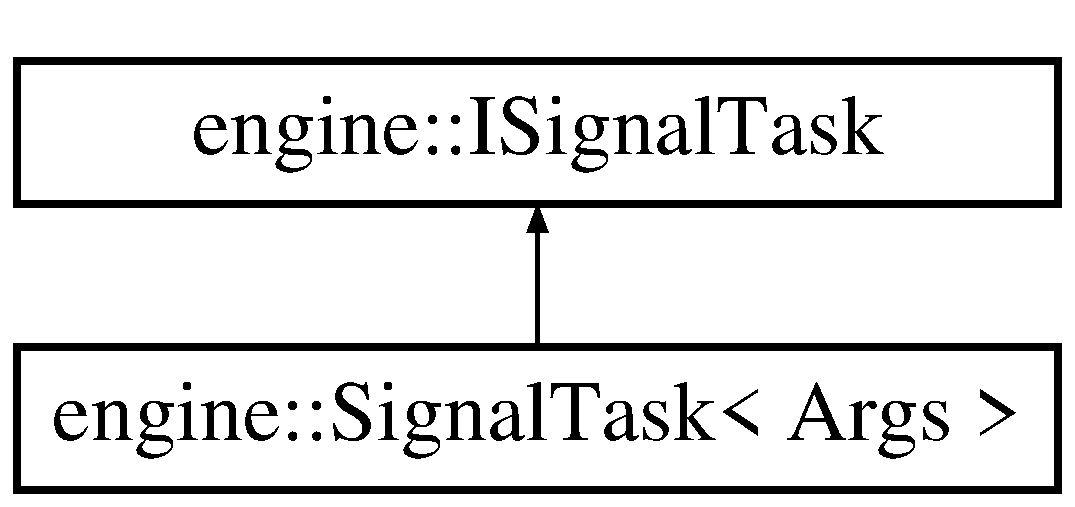
\includegraphics[height=2.000000cm]{a00068}
\end{center}
\end{figure}
\subsubsection*{Public Member Functions}
\begin{DoxyCompactItemize}
\item 
\hyperlink{a00068_aa084db82b7369830ae2121d03c411045}{Signal\+Task} (std\+::weak\+\_\+ptr$<$ \hyperlink{a00066}{Signal\+Caller}$<$ Args... $>$$>$ caller, const std\+::tuple$<$ Args... $>$ \&args)
\item 
void \hyperlink{a00068_a66e71dfc80f4320c2d5c260028b0bbff}{operator()} () override
\item 
bool \hyperlink{a00068_af923108f7304a686bc4b7eeb41c35177}{is\+Expired} () const  override
\end{DoxyCompactItemize}


\subsubsection{Detailed Description}
\subsubsection*{template$<$typename... Args$>$\\*
class engine\+::\+Signal\+Task$<$ Args $>$}

A signal task for the \hyperlink{a00051}{I\+Signal\+Manager}. This class is more than a simple std\+::function because it cares about the object to what the function is bind. 

Definition at line 28 of file Signal\+Task.\+h.



\subsubsection{Constructor \& Destructor Documentation}
\index{engine\+::\+Signal\+Task@{engine\+::\+Signal\+Task}!Signal\+Task@{Signal\+Task}}
\index{Signal\+Task@{Signal\+Task}!engine\+::\+Signal\+Task@{engine\+::\+Signal\+Task}}
\paragraph[{\texorpdfstring{Signal\+Task(std\+::weak\+\_\+ptr$<$ Signal\+Caller$<$ Args... $>$$>$ caller, const std\+::tuple$<$ Args... $>$ \&args)}{SignalTask(std::weak_ptr< SignalCaller< Args... >> caller, const std::tuple< Args... > &args)}}]{\setlength{\rightskip}{0pt plus 5cm}template$<$typename... Args$>$ {\bf engine\+::\+Signal\+Task}$<$ Args $>$\+::{\bf Signal\+Task} (
\begin{DoxyParamCaption}
\item[{std\+::weak\+\_\+ptr$<$ {\bf Signal\+Caller}$<$ Args... $>$$>$}]{caller, }
\item[{const std\+::tuple$<$ Args... $>$ \&}]{args}
\end{DoxyParamCaption}
)\hspace{0.3cm}{\ttfamily [inline]}}\hypertarget{a00068_aa084db82b7369830ae2121d03c411045}{}\label{a00068_aa084db82b7369830ae2121d03c411045}
Create a \hyperlink{a00065}{Signal} task from the weak pointer to the caller and with the arguments. 
\begin{DoxyParams}{Parameters}
{\em caller} & This caller is stored and called. \\
\hline
{\em args} & The caller will called with these arguments. \\
\hline
\end{DoxyParams}


Definition at line 36 of file Signal\+Task.\+h.



\subsubsection{Member Function Documentation}
\index{engine\+::\+Signal\+Task@{engine\+::\+Signal\+Task}!is\+Expired@{is\+Expired}}
\index{is\+Expired@{is\+Expired}!engine\+::\+Signal\+Task@{engine\+::\+Signal\+Task}}
\paragraph[{\texorpdfstring{is\+Expired() const  override}{isExpired() const  override}}]{\setlength{\rightskip}{0pt plus 5cm}template$<$typename... Args$>$ bool {\bf engine\+::\+Signal\+Task}$<$ Args $>$\+::is\+Expired (
\begin{DoxyParamCaption}
{}
\end{DoxyParamCaption}
) const\hspace{0.3cm}{\ttfamily [inline]}, {\ttfamily [override]}, {\ttfamily [virtual]}}\hypertarget{a00068_af923108f7304a686bc4b7eeb41c35177}{}\label{a00068_af923108f7304a686bc4b7eeb41c35177}
Checks whether the pointer to the caller is still valid. 

Implements \hyperlink{a00052_aaa397480f1ad28755a63ad1dca559d50}{engine\+::\+I\+Signal\+Task}.



Definition at line 54 of file Signal\+Task.\+h.

\index{engine\+::\+Signal\+Task@{engine\+::\+Signal\+Task}!operator()@{operator()}}
\index{operator()@{operator()}!engine\+::\+Signal\+Task@{engine\+::\+Signal\+Task}}
\paragraph[{\texorpdfstring{operator()() override}{operator()() override}}]{\setlength{\rightskip}{0pt plus 5cm}template$<$typename... Args$>$ void {\bf engine\+::\+Signal\+Task}$<$ Args $>$\+::operator() (
\begin{DoxyParamCaption}
{}
\end{DoxyParamCaption}
)\hspace{0.3cm}{\ttfamily [inline]}, {\ttfamily [override]}, {\ttfamily [virtual]}}\hypertarget{a00068_a66e71dfc80f4320c2d5c260028b0bbff}{}\label{a00068_a66e71dfc80f4320c2d5c260028b0bbff}
Call the function caller with the stored arguments, but only if the pointer is still valid. 

Implements \hyperlink{a00052_ab7e5dedd50f908fdb0f203b0a154db54}{engine\+::\+I\+Signal\+Task}.



Definition at line 45 of file Signal\+Task.\+h.



The documentation for this class was generated from the following file\+:\begin{DoxyCompactItemize}
\item 
E\+:/\+Programing/\+Projects/\+Engine\+Workspace/\+Common\+Libs/engine/include/engine/signal\+Slot/Signal\+Task.\+h\end{DoxyCompactItemize}

\hypertarget{a00069}{}\subsection{engine\+:\+:Singleton$<$ T $>$ Class Template Reference}
\label{a00069}\index{engine\+::\+Singleton$<$ T $>$@{engine\+::\+Singleton$<$ T $>$}}


{\ttfamily \#include $<$E\+:/\+Programing/\+Projects/\+Engine\+Workspace/\+Common\+Libs/engine/include/engine/constraints/\+Singleton.\+h$>$}

Inheritance diagram for engine\+:\+:Singleton$<$ T $>$\+:\begin{figure}[H]
\begin{center}
\leavevmode
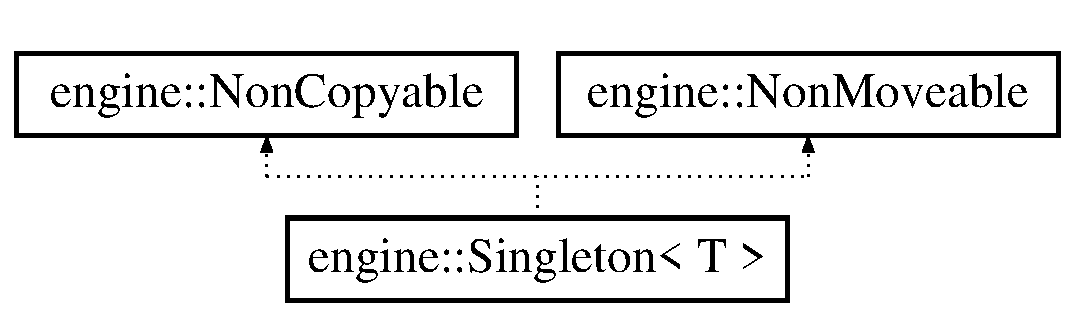
\includegraphics[height=2.000000cm]{a00069}
\end{center}
\end{figure}
\subsubsection*{Static Public Member Functions}
\begin{DoxyCompactItemize}
\item 
static T $\ast$ \hyperlink{a00069_a90ed1f21b1811a569eafccc78fcd12ca}{get\+Instance} ()
\item 
{\footnotesize template$<$typename... Args$>$ }\\static void \hyperlink{a00069_a571e434c8ff771bf65de40f8a7b22076}{create\+Instance} (Args...\+args)
\item 
static void \hyperlink{a00069_a3fbed1f6a78cdf1d0c11467a3be61841}{release\+Instance} ()
\end{DoxyCompactItemize}


\subsubsection{Detailed Description}
\subsubsection*{template$<$class T$>$\\*
class engine\+::\+Singleton$<$ T $>$}

\hyperlink{a00069}{Singleton} implementation 

Definition at line 12 of file Singleton.\+h.



\subsubsection{Member Function Documentation}
\index{engine\+::\+Singleton@{engine\+::\+Singleton}!create\+Instance@{create\+Instance}}
\index{create\+Instance@{create\+Instance}!engine\+::\+Singleton@{engine\+::\+Singleton}}
\paragraph[{\texorpdfstring{create\+Instance(\+Args...\+args)}{createInstance(Args...args)}}]{\setlength{\rightskip}{0pt plus 5cm}template$<$class T$>$ template$<$typename... Args$>$ static void {\bf engine\+::\+Singleton}$<$ T $>$\+::create\+Instance (
\begin{DoxyParamCaption}
\item[{Args...}]{args}
\end{DoxyParamCaption}
)\hspace{0.3cm}{\ttfamily [static]}}\hypertarget{a00069_a571e434c8ff771bf65de40f8a7b22076}{}\label{a00069_a571e434c8ff771bf65de40f8a7b22076}
Create an instance with the given arguments 
\begin{DoxyParams}{Parameters}
{\em creation} & arguments \\
\hline
\end{DoxyParams}
\index{engine\+::\+Singleton@{engine\+::\+Singleton}!get\+Instance@{get\+Instance}}
\index{get\+Instance@{get\+Instance}!engine\+::\+Singleton@{engine\+::\+Singleton}}
\paragraph[{\texorpdfstring{get\+Instance()}{getInstance()}}]{\setlength{\rightskip}{0pt plus 5cm}template$<$class T$>$ static T$\ast$ {\bf engine\+::\+Singleton}$<$ T $>$\+::get\+Instance (
\begin{DoxyParamCaption}
{}
\end{DoxyParamCaption}
)\hspace{0.3cm}{\ttfamily [static]}}\hypertarget{a00069_a90ed1f21b1811a569eafccc78fcd12ca}{}\label{a00069_a90ed1f21b1811a569eafccc78fcd12ca}
\begin{DoxyReturn}{Returns}
the instance object 
\end{DoxyReturn}
\index{engine\+::\+Singleton@{engine\+::\+Singleton}!release\+Instance@{release\+Instance}}
\index{release\+Instance@{release\+Instance}!engine\+::\+Singleton@{engine\+::\+Singleton}}
\paragraph[{\texorpdfstring{release\+Instance()}{releaseInstance()}}]{\setlength{\rightskip}{0pt plus 5cm}template$<$class T$>$ static void {\bf engine\+::\+Singleton}$<$ T $>$\+::release\+Instance (
\begin{DoxyParamCaption}
{}
\end{DoxyParamCaption}
)\hspace{0.3cm}{\ttfamily [static]}}\hypertarget{a00069_a3fbed1f6a78cdf1d0c11467a3be61841}{}\label{a00069_a3fbed1f6a78cdf1d0c11467a3be61841}
Delete the instance 

The documentation for this class was generated from the following file\+:\begin{DoxyCompactItemize}
\item 
E\+:/\+Programing/\+Projects/\+Engine\+Workspace/\+Common\+Libs/engine/include/engine/constraints/Singleton.\+h\end{DoxyCompactItemize}

\hypertarget{a00070}{}\subsection{engine\+:\+:Slot\+Holder Class Reference}
\label{a00070}\index{engine\+::\+Slot\+Holder@{engine\+::\+Slot\+Holder}}


{\ttfamily \#include $<$E\+:/\+Programing/\+Projects/\+Engine\+Workspace/\+Common\+Libs/engine/include/engine/signal\+Slot/\+Slot\+Holder.\+h$>$}

Inheritance diagram for engine\+:\+:Slot\+Holder\+:\begin{figure}[H]
\begin{center}
\leavevmode
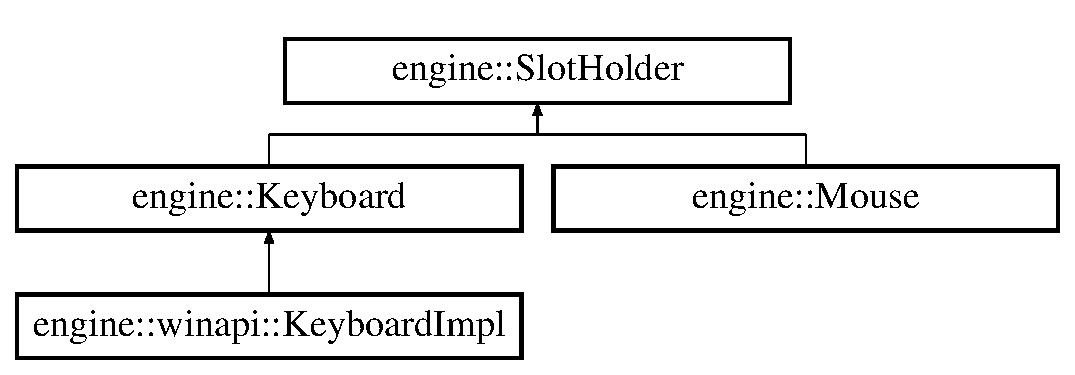
\includegraphics[height=3.000000cm]{a00070}
\end{center}
\end{figure}
\subsubsection*{Public Member Functions}
\begin{DoxyCompactItemize}
\item 
virtual \hyperlink{a00051}{I\+Signal\+Manager} $\ast$ \hyperlink{a00070_add6d89f31a2677b29a52f241d0431c13}{get\+Signal\+Manager} () const  =0
\item 
void \hyperlink{a00070_afd9ce54a72b4dd397d82aff6c387d0c0}{assign\+Signal} (\hyperlink{a00050}{I\+Signal} $\ast$signal)
\item 
void \hyperlink{a00070_a5927b57f0d4fb8744dc0e8ec265e0136}{remove\+Signal} (\hyperlink{a00050}{I\+Signal} $\ast$signal)
\end{DoxyCompactItemize}


\subsubsection{Detailed Description}
To handle emitted signals a kind of \hyperlink{a00065}{Signal} Manager is necessary. To fix the interface inherit your slot holders from this class. 

Definition at line 16 of file Slot\+Holder.\+h.



\subsubsection{Member Function Documentation}
\index{engine\+::\+Slot\+Holder@{engine\+::\+Slot\+Holder}!assign\+Signal@{assign\+Signal}}
\index{assign\+Signal@{assign\+Signal}!engine\+::\+Slot\+Holder@{engine\+::\+Slot\+Holder}}
\paragraph[{\texorpdfstring{assign\+Signal(\+I\+Signal $\ast$signal)}{assignSignal(ISignal *signal)}}]{\setlength{\rightskip}{0pt plus 5cm}void engine\+::\+Slot\+Holder\+::assign\+Signal (
\begin{DoxyParamCaption}
\item[{{\bf I\+Signal} $\ast$}]{signal}
\end{DoxyParamCaption}
)}\hypertarget{a00070_afd9ce54a72b4dd397d82aff6c387d0c0}{}\label{a00070_afd9ce54a72b4dd397d82aff6c387d0c0}
Assign a signal to this slot. It is necessery because when this object is destroyed, it must tell to the signal that\textquotesingle{}s not alived. \index{engine\+::\+Slot\+Holder@{engine\+::\+Slot\+Holder}!get\+Signal\+Manager@{get\+Signal\+Manager}}
\index{get\+Signal\+Manager@{get\+Signal\+Manager}!engine\+::\+Slot\+Holder@{engine\+::\+Slot\+Holder}}
\paragraph[{\texorpdfstring{get\+Signal\+Manager() const  =0}{getSignalManager() const  =0}}]{\setlength{\rightskip}{0pt plus 5cm}virtual {\bf I\+Signal\+Manager}$\ast$ engine\+::\+Slot\+Holder\+::get\+Signal\+Manager (
\begin{DoxyParamCaption}
{}
\end{DoxyParamCaption}
) const\hspace{0.3cm}{\ttfamily [pure virtual]}}\hypertarget{a00070_add6d89f31a2677b29a52f241d0431c13}{}\label{a00070_add6d89f31a2677b29a52f241d0431c13}
\begin{DoxyReturn}{Returns}
Returns the corresponding \hyperlink{a00067}{Signal\+Manager}, who will manage the tasks. 
\end{DoxyReturn}


Implemented in \hyperlink{a00055_a324f41177f75c6d08ad6494c36a65806}{engine\+::\+Keyboard}, and \hyperlink{a00057_a655d612dbf601fec2b116a1c94198247}{engine\+::\+Mouse}.

\index{engine\+::\+Slot\+Holder@{engine\+::\+Slot\+Holder}!remove\+Signal@{remove\+Signal}}
\index{remove\+Signal@{remove\+Signal}!engine\+::\+Slot\+Holder@{engine\+::\+Slot\+Holder}}
\paragraph[{\texorpdfstring{remove\+Signal(\+I\+Signal $\ast$signal)}{removeSignal(ISignal *signal)}}]{\setlength{\rightskip}{0pt plus 5cm}void engine\+::\+Slot\+Holder\+::remove\+Signal (
\begin{DoxyParamCaption}
\item[{{\bf I\+Signal} $\ast$}]{signal}
\end{DoxyParamCaption}
)}\hypertarget{a00070_a5927b57f0d4fb8744dc0e8ec265e0136}{}\label{a00070_a5927b57f0d4fb8744dc0e8ec265e0136}
Remove signal from this slots. 

The documentation for this class was generated from the following file\+:\begin{DoxyCompactItemize}
\item 
E\+:/\+Programing/\+Projects/\+Engine\+Workspace/\+Common\+Libs/engine/include/engine/signal\+Slot/\hyperlink{a00141}{Slot\+Holder.\+h}\end{DoxyCompactItemize}

\hypertarget{a00071}{}\subsection{engine\+:\+:Standard\+Application\+Parameter Class Reference}
\label{a00071}\index{engine\+::\+Standard\+Application\+Parameter@{engine\+::\+Standard\+Application\+Parameter}}


{\ttfamily \#include $<$E\+:/\+Programing/\+Projects/\+Engine\+Workspace/\+Common\+Libs/engine/include/engine/app/\+Standard\+Application\+Parameter.\+h$>$}

Inheritance diagram for engine\+:\+:Standard\+Application\+Parameter\+:\begin{figure}[H]
\begin{center}
\leavevmode
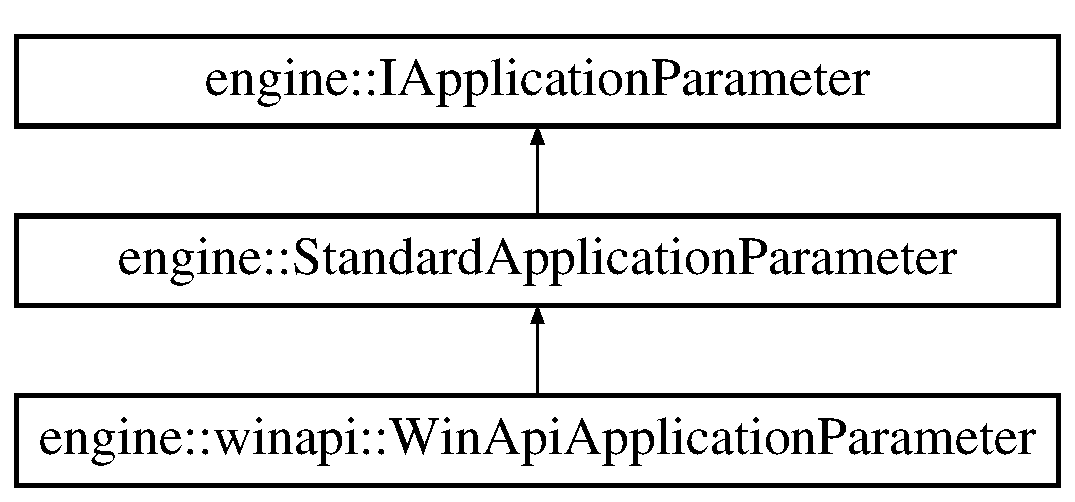
\includegraphics[height=3.000000cm]{a00071}
\end{center}
\end{figure}
\subsubsection*{Public Member Functions}
\begin{DoxyCompactItemize}
\item 
\hyperlink{a00071_ab0088697771492ee97bdaa9b09a97c08}{Standard\+Application\+Parameter} (uint32\+\_\+t n\+Params, char $\ast$parameters\mbox{[}$\,$\mbox{]})
\item 
\hyperlink{a00071_a91c65b5c5cc6c87005fb618b61daef5a}{$\sim$\+Standard\+Application\+Parameter} () override
\item 
const std\+::vector$<$ std\+::string $>$ \& \hyperlink{a00071_ae482854d2439758cfd1d2c710c621b4f}{get\+Parameters} () const 
\item 
const std\+::string \& \hyperlink{a00071_a5d29ea3dfb725dc1a386926896b5a48a}{get\+Binary\+Name} () const 
\end{DoxyCompactItemize}
\subsubsection*{Protected Member Functions}
\begin{DoxyCompactItemize}
\item 
\hyperlink{a00071_ab09e6ae2065a3a1e1fc4461d5f25c46b}{Standard\+Application\+Parameter} ()
\item 
void \hyperlink{a00071_aaf7d27892d7fbad5573099a4fabb6218}{init} (uint32\+\_\+t n\+Params, const std\+::vector$<$ std\+::string $>$ \&parameters)
\end{DoxyCompactItemize}


\subsubsection{Detailed Description}
Standard application parameter representation. For main(int argc, char $\ast$$\ast$args) type main functions 

Definition at line 10 of file Standard\+Application\+Parameter.\+h.



\subsubsection{Constructor \& Destructor Documentation}
\index{engine\+::\+Standard\+Application\+Parameter@{engine\+::\+Standard\+Application\+Parameter}!Standard\+Application\+Parameter@{Standard\+Application\+Parameter}}
\index{Standard\+Application\+Parameter@{Standard\+Application\+Parameter}!engine\+::\+Standard\+Application\+Parameter@{engine\+::\+Standard\+Application\+Parameter}}
\paragraph[{\texorpdfstring{Standard\+Application\+Parameter(uint32\+\_\+t n\+Params, char $\ast$parameters[])}{StandardApplicationParameter(uint32_t nParams, char *parameters[])}}]{\setlength{\rightskip}{0pt plus 5cm}engine\+::\+Standard\+Application\+Parameter\+::\+Standard\+Application\+Parameter (
\begin{DoxyParamCaption}
\item[{uint32\+\_\+t}]{n\+Params, }
\item[{char $\ast$}]{parameters\mbox{[}$\,$\mbox{]}}
\end{DoxyParamCaption}
)}\hypertarget{a00071_ab0088697771492ee97bdaa9b09a97c08}{}\label{a00071_ab0088697771492ee97bdaa9b09a97c08}
Create a standard parameter representation 
\begin{DoxyParams}{Parameters}
{\em n\+Params} & number of parameters \\
\hline
{\em parameters} & Parameters array with length n\+Params \\
\hline
\end{DoxyParams}
\index{engine\+::\+Standard\+Application\+Parameter@{engine\+::\+Standard\+Application\+Parameter}!Standard\+Application\+Parameter@{Standard\+Application\+Parameter}}
\index{Standard\+Application\+Parameter@{Standard\+Application\+Parameter}!engine\+::\+Standard\+Application\+Parameter@{engine\+::\+Standard\+Application\+Parameter}}
\paragraph[{\texorpdfstring{Standard\+Application\+Parameter()}{StandardApplicationParameter()}}]{\setlength{\rightskip}{0pt plus 5cm}engine\+::\+Standard\+Application\+Parameter\+::\+Standard\+Application\+Parameter (
\begin{DoxyParamCaption}
{}
\end{DoxyParamCaption}
)\hspace{0.3cm}{\ttfamily [protected]}}\hypertarget{a00071_ab09e6ae2065a3a1e1fc4461d5f25c46b}{}\label{a00071_ab09e6ae2065a3a1e1fc4461d5f25c46b}
For child classes it is possible to empty initialization. \index{engine\+::\+Standard\+Application\+Parameter@{engine\+::\+Standard\+Application\+Parameter}!````~Standard\+Application\+Parameter@{$\sim$\+Standard\+Application\+Parameter}}
\index{````~Standard\+Application\+Parameter@{$\sim$\+Standard\+Application\+Parameter}!engine\+::\+Standard\+Application\+Parameter@{engine\+::\+Standard\+Application\+Parameter}}
\paragraph[{\texorpdfstring{$\sim$\+Standard\+Application\+Parameter() override}{~StandardApplicationParameter() override}}]{\setlength{\rightskip}{0pt plus 5cm}engine\+::\+Standard\+Application\+Parameter\+::$\sim$\+Standard\+Application\+Parameter (
\begin{DoxyParamCaption}
{}
\end{DoxyParamCaption}
)\hspace{0.3cm}{\ttfamily [override]}}\hypertarget{a00071_a91c65b5c5cc6c87005fb618b61daef5a}{}\label{a00071_a91c65b5c5cc6c87005fb618b61daef5a}
Destructor for P\+I\+M\+PL 

\subsubsection{Member Function Documentation}
\index{engine\+::\+Standard\+Application\+Parameter@{engine\+::\+Standard\+Application\+Parameter}!get\+Binary\+Name@{get\+Binary\+Name}}
\index{get\+Binary\+Name@{get\+Binary\+Name}!engine\+::\+Standard\+Application\+Parameter@{engine\+::\+Standard\+Application\+Parameter}}
\paragraph[{\texorpdfstring{get\+Binary\+Name() const }{getBinaryName() const }}]{\setlength{\rightskip}{0pt plus 5cm}const std\+::string\& engine\+::\+Standard\+Application\+Parameter\+::get\+Binary\+Name (
\begin{DoxyParamCaption}
{}
\end{DoxyParamCaption}
) const}\hypertarget{a00071_a5d29ea3dfb725dc1a386926896b5a48a}{}\label{a00071_a5d29ea3dfb725dc1a386926896b5a48a}
\begin{DoxyReturn}{Returns}
Returns the name of the binary 
\end{DoxyReturn}
\index{engine\+::\+Standard\+Application\+Parameter@{engine\+::\+Standard\+Application\+Parameter}!get\+Parameters@{get\+Parameters}}
\index{get\+Parameters@{get\+Parameters}!engine\+::\+Standard\+Application\+Parameter@{engine\+::\+Standard\+Application\+Parameter}}
\paragraph[{\texorpdfstring{get\+Parameters() const }{getParameters() const }}]{\setlength{\rightskip}{0pt plus 5cm}const std\+::vector$<$std\+::string$>$\& engine\+::\+Standard\+Application\+Parameter\+::get\+Parameters (
\begin{DoxyParamCaption}
{}
\end{DoxyParamCaption}
) const}\hypertarget{a00071_ae482854d2439758cfd1d2c710c621b4f}{}\label{a00071_ae482854d2439758cfd1d2c710c621b4f}
\begin{DoxyReturn}{Returns}
Returns the parameters in a vector 
\end{DoxyReturn}
\index{engine\+::\+Standard\+Application\+Parameter@{engine\+::\+Standard\+Application\+Parameter}!init@{init}}
\index{init@{init}!engine\+::\+Standard\+Application\+Parameter@{engine\+::\+Standard\+Application\+Parameter}}
\paragraph[{\texorpdfstring{init(uint32\+\_\+t n\+Params, const std\+::vector$<$ std\+::string $>$ \&parameters)}{init(uint32_t nParams, const std::vector< std::string > &parameters)}}]{\setlength{\rightskip}{0pt plus 5cm}void engine\+::\+Standard\+Application\+Parameter\+::init (
\begin{DoxyParamCaption}
\item[{uint32\+\_\+t}]{n\+Params, }
\item[{const std\+::vector$<$ std\+::string $>$ \&}]{parameters}
\end{DoxyParamCaption}
)\hspace{0.3cm}{\ttfamily [protected]}}\hypertarget{a00071_aaf7d27892d7fbad5573099a4fabb6218}{}\label{a00071_aaf7d27892d7fbad5573099a4fabb6218}
Function for initialize the members 

The documentation for this class was generated from the following file\+:\begin{DoxyCompactItemize}
\item 
E\+:/\+Programing/\+Projects/\+Engine\+Workspace/\+Common\+Libs/engine/include/engine/app/Standard\+Application\+Parameter.\+h\end{DoxyCompactItemize}

\hypertarget{a00072}{}\subsection{engine\+:\+:State\+Base Class Reference}
\label{a00072}\index{engine\+::\+State\+Base@{engine\+::\+State\+Base}}


{\ttfamily \#include $<$E\+:/\+Programing/\+Projects/\+Engine\+Workspace/\+Common\+Libs/engine/include/engine/state\+Stack/\+State\+Base.\+h$>$}

Inheritance diagram for engine\+:\+:State\+Base\+:\begin{figure}[H]
\begin{center}
\leavevmode
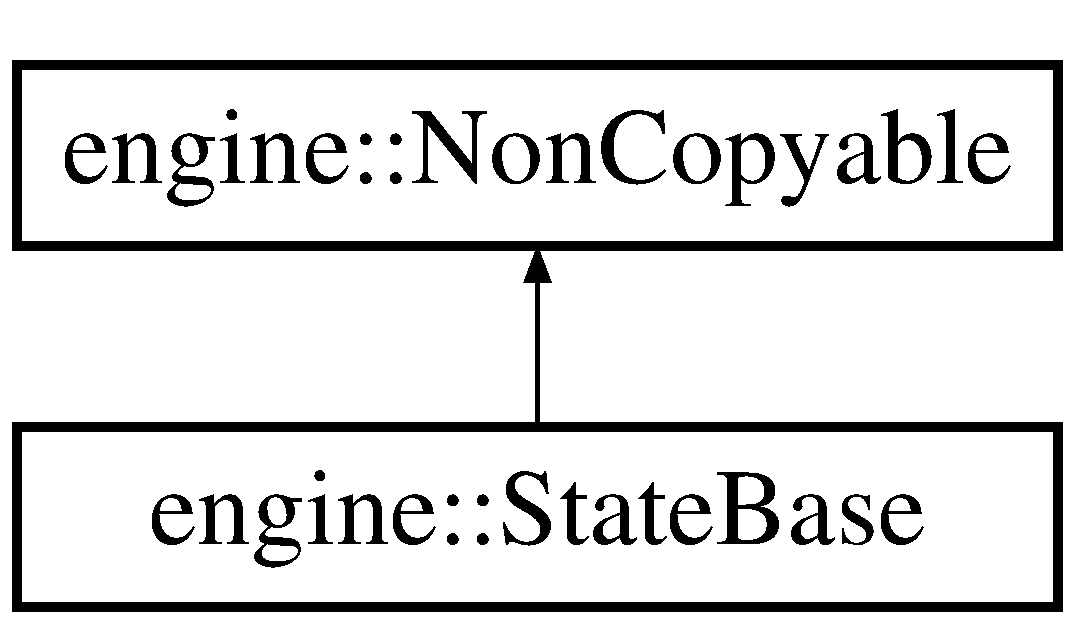
\includegraphics[height=2.000000cm]{a00072}
\end{center}
\end{figure}
\subsubsection*{Public Member Functions}
\begin{DoxyCompactItemize}
\item 
virtual \hyperlink{a00072_ab664691d7ef22f9764816ab9aaf7d537}{$\sim$\+State\+Base} ()
\item 
void \hyperlink{a00072_aa80ea4f74acd99c5b51d61e397b84e0b}{initialize} (\hyperlink{a00073}{State\+Stack} $\ast$stack)
\item 
void \hyperlink{a00072_a28c40b43d8852235b3f2ea4ca39c0cad}{destroy} ()
\item 
void \hyperlink{a00072_a7a109867f252655aa625f8421071fa23}{resume} ()
\item 
void \hyperlink{a00072_acc1a281ee5cd9192fb7a703c5ef8c49b}{pause} ()
\item 
void \hyperlink{a00072_a90b80b1002ed942c2f3b8dd9965cfba0}{update} ()
\item 
void \hyperlink{a00072_a0e52521456a98ab4b8a58ba01d356836}{render} ()
\item 
bool \hyperlink{a00072_a73a808c7f866e21ab85b694d726159eb}{is\+Initialized} () const 
\item 
void \hyperlink{a00072_a369f9b474222dfe2109e6d15630157db}{trace} (std\+::ostream \&) const 
\end{DoxyCompactItemize}
\subsubsection*{Protected Member Functions}
\begin{DoxyCompactItemize}
\item 
\hyperlink{a00072_aee338ee916b37c21d986e2f0c6a3cf01}{State\+Base} (const std\+::string \&name)
\item 
bool \hyperlink{a00072_a9dbd0e91cd8812be304df62aa8bca558}{is\+Active} () const 
\item 
bool \hyperlink{a00072_aaec38f3ff2f0af1bffcad4054f92f5f0}{is\+Leaving} () const 
\item 
void \hyperlink{a00072_a95a7fffdec13deafa7855755f6f5f153}{change\+State} (std\+::unique\+\_\+ptr$<$ \hyperlink{a00072}{State\+Base} $>$ next\+State)
\item 
void \hyperlink{a00072_a04227376a170bdb851e0e03a4949f564}{exit\+State} ()
\end{DoxyCompactItemize}
\subsubsection*{Protected Attributes}
\begin{DoxyCompactItemize}
\item 
\hyperlink{a00065}{Signal}$<$ \hyperlink{a00072}{State\+Base} $\ast$ $>$ \hyperlink{a00072_aa585934f221ce16ddac54f79c759e30e}{state\+Changed}
\item 
\hyperlink{a00065}{Signal} \hyperlink{a00072_aa833cf334d703956398b0eab5353fb14}{state\+Terminated}
\end{DoxyCompactItemize}


\subsubsection{Detailed Description}
Base class for game states. This class is managed by the state stack. 

Definition at line 15 of file State\+Base.\+h.



\subsubsection{Constructor \& Destructor Documentation}
\index{engine\+::\+State\+Base@{engine\+::\+State\+Base}!State\+Base@{State\+Base}}
\index{State\+Base@{State\+Base}!engine\+::\+State\+Base@{engine\+::\+State\+Base}}
\paragraph[{\texorpdfstring{State\+Base(const std\+::string \&name)}{StateBase(const std::string &name)}}]{\setlength{\rightskip}{0pt plus 5cm}engine\+::\+State\+Base\+::\+State\+Base (
\begin{DoxyParamCaption}
\item[{const std\+::string \&}]{name}
\end{DoxyParamCaption}
)\hspace{0.3cm}{\ttfamily [protected]}}\hypertarget{a00072_aee338ee916b37c21d986e2f0c6a3cf01}{}\label{a00072_aee338ee916b37c21d986e2f0c6a3cf01}
Construct a state. The object must not been initialized by the constructor, it can be done during initialization. \begin{DoxySeeAlso}{See also}

\end{DoxySeeAlso}
\index{engine\+::\+State\+Base@{engine\+::\+State\+Base}!````~State\+Base@{$\sim$\+State\+Base}}
\index{````~State\+Base@{$\sim$\+State\+Base}!engine\+::\+State\+Base@{engine\+::\+State\+Base}}
\paragraph[{\texorpdfstring{$\sim$\+State\+Base()}{~StateBase()}}]{\setlength{\rightskip}{0pt plus 5cm}virtual engine\+::\+State\+Base\+::$\sim$\+State\+Base (
\begin{DoxyParamCaption}
{}
\end{DoxyParamCaption}
)\hspace{0.3cm}{\ttfamily [virtual]}}\hypertarget{a00072_ab664691d7ef22f9764816ab9aaf7d537}{}\label{a00072_ab664691d7ef22f9764816ab9aaf7d537}
Destroy the state. The object also can be destroyed by other function simirary as it was in constructed. \begin{DoxySeeAlso}{See also}

\end{DoxySeeAlso}


\subsubsection{Member Function Documentation}
\index{engine\+::\+State\+Base@{engine\+::\+State\+Base}!change\+State@{change\+State}}
\index{change\+State@{change\+State}!engine\+::\+State\+Base@{engine\+::\+State\+Base}}
\paragraph[{\texorpdfstring{change\+State(std\+::unique\+\_\+ptr$<$ State\+Base $>$ next\+State)}{changeState(std::unique_ptr< StateBase > nextState)}}]{\setlength{\rightskip}{0pt plus 5cm}void engine\+::\+State\+Base\+::change\+State (
\begin{DoxyParamCaption}
\item[{std\+::unique\+\_\+ptr$<$ {\bf State\+Base} $>$}]{next\+State}
\end{DoxyParamCaption}
)\hspace{0.3cm}{\ttfamily [protected]}}\hypertarget{a00072_a95a7fffdec13deafa7855755f6f5f153}{}\label{a00072_a95a7fffdec13deafa7855755f6f5f153}
Push an other state to top of the corresponding state stack. 
\begin{DoxyParams}{Parameters}
{\em next\+State} & state which is pushed on the top of the stack. \\
\hline
\end{DoxyParams}
\index{engine\+::\+State\+Base@{engine\+::\+State\+Base}!destroy@{destroy}}
\index{destroy@{destroy}!engine\+::\+State\+Base@{engine\+::\+State\+Base}}
\paragraph[{\texorpdfstring{destroy()}{destroy()}}]{\setlength{\rightskip}{0pt plus 5cm}void engine\+::\+State\+Base\+::destroy (
\begin{DoxyParamCaption}
{}
\end{DoxyParamCaption}
)}\hypertarget{a00072_a28c40b43d8852235b3f2ea4ca39c0cad}{}\label{a00072_a28c40b43d8852235b3f2ea4ca39c0cad}
Destory this state; \index{engine\+::\+State\+Base@{engine\+::\+State\+Base}!exit\+State@{exit\+State}}
\index{exit\+State@{exit\+State}!engine\+::\+State\+Base@{engine\+::\+State\+Base}}
\paragraph[{\texorpdfstring{exit\+State()}{exitState()}}]{\setlength{\rightskip}{0pt plus 5cm}void engine\+::\+State\+Base\+::exit\+State (
\begin{DoxyParamCaption}
{}
\end{DoxyParamCaption}
)\hspace{0.3cm}{\ttfamily [protected]}}\hypertarget{a00072_a04227376a170bdb851e0e03a4949f564}{}\label{a00072_a04227376a170bdb851e0e03a4949f564}
Remove this state from the stack. \begin{DoxyWarning}{Warning}
Only the active state can call this function. 
\end{DoxyWarning}
\index{engine\+::\+State\+Base@{engine\+::\+State\+Base}!initialize@{initialize}}
\index{initialize@{initialize}!engine\+::\+State\+Base@{engine\+::\+State\+Base}}
\paragraph[{\texorpdfstring{initialize(\+State\+Stack $\ast$stack)}{initialize(StateStack *stack)}}]{\setlength{\rightskip}{0pt plus 5cm}void engine\+::\+State\+Base\+::initialize (
\begin{DoxyParamCaption}
\item[{{\bf State\+Stack} $\ast$}]{stack}
\end{DoxyParamCaption}
)}\hypertarget{a00072_aa80ea4f74acd99c5b51d61e397b84e0b}{}\label{a00072_aa80ea4f74acd99c5b51d61e397b84e0b}
This function initialize this state. A state can change the stack and can go another states. It has two possible way push a new state to the stack or remove the current state from the stack. To do this the state must know the corresponding stack. 
\begin{DoxyParams}{Parameters}
{\em stack} & corresponding stack. \\
\hline
\end{DoxyParams}
\index{engine\+::\+State\+Base@{engine\+::\+State\+Base}!is\+Active@{is\+Active}}
\index{is\+Active@{is\+Active}!engine\+::\+State\+Base@{engine\+::\+State\+Base}}
\paragraph[{\texorpdfstring{is\+Active() const }{isActive() const }}]{\setlength{\rightskip}{0pt plus 5cm}bool engine\+::\+State\+Base\+::is\+Active (
\begin{DoxyParamCaption}
{}
\end{DoxyParamCaption}
) const\hspace{0.3cm}{\ttfamily [protected]}}\hypertarget{a00072_a9dbd0e91cd8812be304df62aa8bca558}{}\label{a00072_a9dbd0e91cd8812be304df62aa8bca558}
A state is active when the resume is called on the state but the pause isn\textquotesingle{}t yet. \index{engine\+::\+State\+Base@{engine\+::\+State\+Base}!is\+Initialized@{is\+Initialized}}
\index{is\+Initialized@{is\+Initialized}!engine\+::\+State\+Base@{engine\+::\+State\+Base}}
\paragraph[{\texorpdfstring{is\+Initialized() const }{isInitialized() const }}]{\setlength{\rightskip}{0pt plus 5cm}bool engine\+::\+State\+Base\+::is\+Initialized (
\begin{DoxyParamCaption}
{}
\end{DoxyParamCaption}
) const}\hypertarget{a00072_a73a808c7f866e21ab85b694d726159eb}{}\label{a00072_a73a808c7f866e21ab85b694d726159eb}
\begin{DoxyReturn}{Returns}
true when the state is initialized and not destroyed. 
\end{DoxyReturn}
\index{engine\+::\+State\+Base@{engine\+::\+State\+Base}!is\+Leaving@{is\+Leaving}}
\index{is\+Leaving@{is\+Leaving}!engine\+::\+State\+Base@{engine\+::\+State\+Base}}
\paragraph[{\texorpdfstring{is\+Leaving() const }{isLeaving() const }}]{\setlength{\rightskip}{0pt plus 5cm}bool engine\+::\+State\+Base\+::is\+Leaving (
\begin{DoxyParamCaption}
{}
\end{DoxyParamCaption}
) const\hspace{0.3cm}{\ttfamily [protected]}}\hypertarget{a00072_aaec38f3ff2f0af1bffcad4054f92f5f0}{}\label{a00072_aaec38f3ff2f0af1bffcad4054f92f5f0}
When a state is leaving it\textquotesingle{}s active but in the next frame it won\textquotesingle{}t be at the top of the stack. \begin{DoxyReturn}{Returns}
Returns true when exit or change state has been called already. 
\end{DoxyReturn}
\index{engine\+::\+State\+Base@{engine\+::\+State\+Base}!pause@{pause}}
\index{pause@{pause}!engine\+::\+State\+Base@{engine\+::\+State\+Base}}
\paragraph[{\texorpdfstring{pause()}{pause()}}]{\setlength{\rightskip}{0pt plus 5cm}void engine\+::\+State\+Base\+::pause (
\begin{DoxyParamCaption}
{}
\end{DoxyParamCaption}
)}\hypertarget{a00072_acc1a281ee5cd9192fb7a703c5ef8c49b}{}\label{a00072_acc1a281ee5cd9192fb7a703c5ef8c49b}
Pause is called when a state becomes inactive so when it is not on the top of the stack. It can be done in two way someone is pushed above this state or the current state is popped from the stack. Only initialized states can be paused. \begin{DoxySeeAlso}{See also}
\hyperlink{a00072_a95a7fffdec13deafa7855755f6f5f153}{change\+State} 

\hyperlink{a00072_a04227376a170bdb851e0e03a4949f564}{exit\+State} 
\end{DoxySeeAlso}
\index{engine\+::\+State\+Base@{engine\+::\+State\+Base}!render@{render}}
\index{render@{render}!engine\+::\+State\+Base@{engine\+::\+State\+Base}}
\paragraph[{\texorpdfstring{render()}{render()}}]{\setlength{\rightskip}{0pt plus 5cm}void engine\+::\+State\+Base\+::render (
\begin{DoxyParamCaption}
{}
\end{DoxyParamCaption}
)}\hypertarget{a00072_a0e52521456a98ab4b8a58ba01d356836}{}\label{a00072_a0e52521456a98ab4b8a58ba01d356836}
The active state is rendered in each frame. \index{engine\+::\+State\+Base@{engine\+::\+State\+Base}!resume@{resume}}
\index{resume@{resume}!engine\+::\+State\+Base@{engine\+::\+State\+Base}}
\paragraph[{\texorpdfstring{resume()}{resume()}}]{\setlength{\rightskip}{0pt plus 5cm}void engine\+::\+State\+Base\+::resume (
\begin{DoxyParamCaption}
{}
\end{DoxyParamCaption}
)}\hypertarget{a00072_a7a109867f252655aa625f8421071fa23}{}\label{a00072_a7a109867f252655aa625f8421071fa23}
Resume is called when a state becomes active so when it is on the top of the stack. Only initialized states can be resumed. \index{engine\+::\+State\+Base@{engine\+::\+State\+Base}!trace@{trace}}
\index{trace@{trace}!engine\+::\+State\+Base@{engine\+::\+State\+Base}}
\paragraph[{\texorpdfstring{trace(std\+::ostream \&) const }{trace(std::ostream &) const }}]{\setlength{\rightskip}{0pt plus 5cm}void engine\+::\+State\+Base\+::trace (
\begin{DoxyParamCaption}
\item[{std\+::ostream \&}]{}
\end{DoxyParamCaption}
) const}\hypertarget{a00072_a369f9b474222dfe2109e6d15630157db}{}\label{a00072_a369f9b474222dfe2109e6d15630157db}
trace informations about this state. \index{engine\+::\+State\+Base@{engine\+::\+State\+Base}!update@{update}}
\index{update@{update}!engine\+::\+State\+Base@{engine\+::\+State\+Base}}
\paragraph[{\texorpdfstring{update()}{update()}}]{\setlength{\rightskip}{0pt plus 5cm}void engine\+::\+State\+Base\+::update (
\begin{DoxyParamCaption}
{}
\end{DoxyParamCaption}
)}\hypertarget{a00072_a90b80b1002ed942c2f3b8dd9965cfba0}{}\label{a00072_a90b80b1002ed942c2f3b8dd9965cfba0}
The active state is updated in each frame. 

\subsubsection{Member Data Documentation}
\index{engine\+::\+State\+Base@{engine\+::\+State\+Base}!state\+Changed@{state\+Changed}}
\index{state\+Changed@{state\+Changed}!engine\+::\+State\+Base@{engine\+::\+State\+Base}}
\paragraph[{\texorpdfstring{state\+Changed}{stateChanged}}]{\setlength{\rightskip}{0pt plus 5cm}{\bf Signal}$<${\bf State\+Base}$\ast$$>$ engine\+::\+State\+Base\+::state\+Changed\hspace{0.3cm}{\ttfamily [protected]}}\hypertarget{a00072_aa585934f221ce16ddac54f79c759e30e}{}\label{a00072_aa585934f221ce16ddac54f79c759e30e}
\hyperlink{a00065}{Signal} for state changes to a next state. The parameter is a pointer to the next state. \begin{DoxySeeAlso}{See also}
\hyperlink{a00072_a95a7fffdec13deafa7855755f6f5f153}{change\+State} 
\end{DoxySeeAlso}


Definition at line 129 of file State\+Base.\+h.

\index{engine\+::\+State\+Base@{engine\+::\+State\+Base}!state\+Terminated@{state\+Terminated}}
\index{state\+Terminated@{state\+Terminated}!engine\+::\+State\+Base@{engine\+::\+State\+Base}}
\paragraph[{\texorpdfstring{state\+Terminated}{stateTerminated}}]{\setlength{\rightskip}{0pt plus 5cm}{\bf Signal} engine\+::\+State\+Base\+::state\+Terminated\hspace{0.3cm}{\ttfamily [protected]}}\hypertarget{a00072_aa833cf334d703956398b0eab5353fb14}{}\label{a00072_aa833cf334d703956398b0eab5353fb14}
\hyperlink{a00065}{Signal} for state exit. \begin{DoxySeeAlso}{See also}
\hyperlink{a00072_a04227376a170bdb851e0e03a4949f564}{exit\+State} 
\end{DoxySeeAlso}


Definition at line 138 of file State\+Base.\+h.



The documentation for this class was generated from the following file\+:\begin{DoxyCompactItemize}
\item 
E\+:/\+Programing/\+Projects/\+Engine\+Workspace/\+Common\+Libs/engine/include/engine/state\+Stack/State\+Base.\+h\end{DoxyCompactItemize}

\hypertarget{a00073}{}\subsection{engine\+:\+:State\+Stack Class Reference}
\label{a00073}\index{engine\+::\+State\+Stack@{engine\+::\+State\+Stack}}


{\ttfamily \#include $<$E\+:/\+Programing/\+Projects/\+Engine\+Workspace/\+Common\+Libs/engine/include/engine/state\+Stack/\+State\+Stack.\+h$>$}

Inheritance diagram for engine\+:\+:State\+Stack\+:\begin{figure}[H]
\begin{center}
\leavevmode
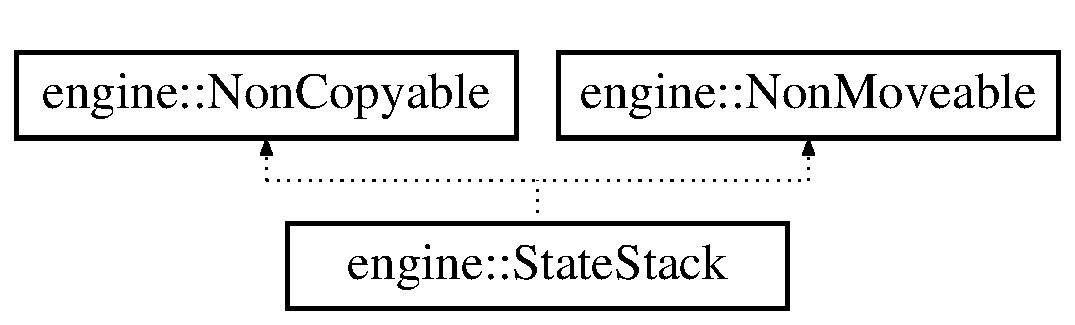
\includegraphics[height=2.000000cm]{a00073}
\end{center}
\end{figure}
\subsubsection*{Public Types}
\begin{DoxyCompactItemize}
\item 
using \hyperlink{a00073_a866f3ce726d328dc3488f3300b94be07}{State\+List} = std\+::list$<$ \hyperlink{a00072}{State\+Base} $\ast$ $>$
\end{DoxyCompactItemize}
\subsubsection*{Public Member Functions}
\begin{DoxyCompactItemize}
\item 
\hyperlink{a00073_af80814eae37384bbbf07f3c041ff9489}{State\+Stack} ()
\item 
\hyperlink{a00073_a1c5c62604825cc9e4395212cd2986829}{$\sim$\+State\+Stack} ()
\item 
void \hyperlink{a00073_a129b751979654c033dfbb5595519db48}{update} ()
\item 
void \hyperlink{a00073_a948f666845a6bbebc6f629a3eef8de0b}{render} ()
\item 
void \hyperlink{a00073_aae3b3caef3cf8dfd7ba9ea0232b5babd}{push\+State} (std\+::unique\+\_\+ptr$<$ \hyperlink{a00072}{State\+Base} $>$ state)
\item 
void \hyperlink{a00073_ad4332c156e0169fcde04044acb59928d}{pop\+State} ()
\item 
void \hyperlink{a00073_a7d05f3d0f8ca93a48911bb14558314d4}{trace} (std\+::ostream \&os) const 
\item 
bool \hyperlink{a00073_a07e9947e97bb7e5ad5533d68f0791429}{is\+Empty} () const 
\end{DoxyCompactItemize}


\subsubsection{Detailed Description}
This class is responsible to handle game state changes. This stack has 2 face, one is not midified during the current frame execution, the other one is changing when push or pop is called. At the begining of the frame the update of the stack is called and it applies the modification what was done in the previous frame. 

Definition at line 18 of file State\+Stack.\+h.



\subsubsection{Member Typedef Documentation}
\index{engine\+::\+State\+Stack@{engine\+::\+State\+Stack}!State\+List@{State\+List}}
\index{State\+List@{State\+List}!engine\+::\+State\+Stack@{engine\+::\+State\+Stack}}
\paragraph[{\texorpdfstring{State\+List}{StateList}}]{\setlength{\rightskip}{0pt plus 5cm}using {\bf engine\+::\+State\+Stack\+::\+State\+List} =  std\+::list $<$ {\bf State\+Base}$\ast$ $>$}\hypertarget{a00073_a866f3ce726d328dc3488f3300b94be07}{}\label{a00073_a866f3ce726d328dc3488f3300b94be07}
Container for states 

Definition at line 24 of file State\+Stack.\+h.



\subsubsection{Constructor \& Destructor Documentation}
\index{engine\+::\+State\+Stack@{engine\+::\+State\+Stack}!State\+Stack@{State\+Stack}}
\index{State\+Stack@{State\+Stack}!engine\+::\+State\+Stack@{engine\+::\+State\+Stack}}
\paragraph[{\texorpdfstring{State\+Stack()}{StateStack()}}]{\setlength{\rightskip}{0pt plus 5cm}engine\+::\+State\+Stack\+::\+State\+Stack (
\begin{DoxyParamCaption}
{}
\end{DoxyParamCaption}
)}\hypertarget{a00073_af80814eae37384bbbf07f3c041ff9489}{}\label{a00073_af80814eae37384bbbf07f3c041ff9489}
Default constuctor \index{engine\+::\+State\+Stack@{engine\+::\+State\+Stack}!````~State\+Stack@{$\sim$\+State\+Stack}}
\index{````~State\+Stack@{$\sim$\+State\+Stack}!engine\+::\+State\+Stack@{engine\+::\+State\+Stack}}
\paragraph[{\texorpdfstring{$\sim$\+State\+Stack()}{~StateStack()}}]{\setlength{\rightskip}{0pt plus 5cm}engine\+::\+State\+Stack\+::$\sim$\+State\+Stack (
\begin{DoxyParamCaption}
{}
\end{DoxyParamCaption}
)}\hypertarget{a00073_a1c5c62604825cc9e4395212cd2986829}{}\label{a00073_a1c5c62604825cc9e4395212cd2986829}
Non virtual destructor. Further inheritance is not allowed. 

\subsubsection{Member Function Documentation}
\index{engine\+::\+State\+Stack@{engine\+::\+State\+Stack}!is\+Empty@{is\+Empty}}
\index{is\+Empty@{is\+Empty}!engine\+::\+State\+Stack@{engine\+::\+State\+Stack}}
\paragraph[{\texorpdfstring{is\+Empty() const }{isEmpty() const }}]{\setlength{\rightskip}{0pt plus 5cm}bool engine\+::\+State\+Stack\+::is\+Empty (
\begin{DoxyParamCaption}
{}
\end{DoxyParamCaption}
) const}\hypertarget{a00073_a07e9947e97bb7e5ad5533d68f0791429}{}\label{a00073_a07e9947e97bb7e5ad5533d68f0791429}
\begin{DoxyReturn}{Returns}
Returns true if it is empty. 
\end{DoxyReturn}
\begin{DoxyWarning}{Warning}
The stack is constant in the frame, so pop end push functions are ignored and this function returns the top of the previous frame. 
\end{DoxyWarning}
\index{engine\+::\+State\+Stack@{engine\+::\+State\+Stack}!pop\+State@{pop\+State}}
\index{pop\+State@{pop\+State}!engine\+::\+State\+Stack@{engine\+::\+State\+Stack}}
\paragraph[{\texorpdfstring{pop\+State()}{popState()}}]{\setlength{\rightskip}{0pt plus 5cm}void engine\+::\+State\+Stack\+::pop\+State (
\begin{DoxyParamCaption}
{}
\end{DoxyParamCaption}
)}\hypertarget{a00073_ad4332c156e0169fcde04044acb59928d}{}\label{a00073_ad4332c156e0169fcde04044acb59928d}
Pops the top from the stack. \begin{DoxyWarning}{Warning}
This function will be applied only in the next frame. 
\end{DoxyWarning}
\index{engine\+::\+State\+Stack@{engine\+::\+State\+Stack}!push\+State@{push\+State}}
\index{push\+State@{push\+State}!engine\+::\+State\+Stack@{engine\+::\+State\+Stack}}
\paragraph[{\texorpdfstring{push\+State(std\+::unique\+\_\+ptr$<$ State\+Base $>$ state)}{pushState(std::unique_ptr< StateBase > state)}}]{\setlength{\rightskip}{0pt plus 5cm}void engine\+::\+State\+Stack\+::push\+State (
\begin{DoxyParamCaption}
\item[{std\+::unique\+\_\+ptr$<$ {\bf State\+Base} $>$}]{state}
\end{DoxyParamCaption}
)}\hypertarget{a00073_aae3b3caef3cf8dfd7ba9ea0232b5babd}{}\label{a00073_aae3b3caef3cf8dfd7ba9ea0232b5babd}
Pushes a new state to the top of the stack. 
\begin{DoxyParams}{Parameters}
{\em state} & State to push to the top. \\
\hline
\end{DoxyParams}
\begin{DoxyWarning}{Warning}
This function will be applied only in the next frame. 
\end{DoxyWarning}
\index{engine\+::\+State\+Stack@{engine\+::\+State\+Stack}!render@{render}}
\index{render@{render}!engine\+::\+State\+Stack@{engine\+::\+State\+Stack}}
\paragraph[{\texorpdfstring{render()}{render()}}]{\setlength{\rightskip}{0pt plus 5cm}void engine\+::\+State\+Stack\+::render (
\begin{DoxyParamCaption}
{}
\end{DoxyParamCaption}
)}\hypertarget{a00073_a948f666845a6bbebc6f629a3eef8de0b}{}\label{a00073_a948f666845a6bbebc6f629a3eef8de0b}
Render the top state if it exists. \index{engine\+::\+State\+Stack@{engine\+::\+State\+Stack}!trace@{trace}}
\index{trace@{trace}!engine\+::\+State\+Stack@{engine\+::\+State\+Stack}}
\paragraph[{\texorpdfstring{trace(std\+::ostream \&os) const }{trace(std::ostream &os) const }}]{\setlength{\rightskip}{0pt plus 5cm}void engine\+::\+State\+Stack\+::trace (
\begin{DoxyParamCaption}
\item[{std\+::ostream \&}]{os}
\end{DoxyParamCaption}
) const}\hypertarget{a00073_a7d05f3d0f8ca93a48911bb14558314d4}{}\label{a00073_a7d05f3d0f8ca93a48911bb14558314d4}
Trace the states in the container. 
\begin{DoxyParams}{Parameters}
{\em os} & stream where data will dumped. \\
\hline
\end{DoxyParams}
\index{engine\+::\+State\+Stack@{engine\+::\+State\+Stack}!update@{update}}
\index{update@{update}!engine\+::\+State\+Stack@{engine\+::\+State\+Stack}}
\paragraph[{\texorpdfstring{update()}{update()}}]{\setlength{\rightskip}{0pt plus 5cm}void engine\+::\+State\+Stack\+::update (
\begin{DoxyParamCaption}
{}
\end{DoxyParamCaption}
)}\hypertarget{a00073_a129b751979654c033dfbb5595519db48}{}\label{a00073_a129b751979654c033dfbb5595519db48}
Update the stack. All the modifications from the previous frame will be applied in this function, and calls the top state\textquotesingle{}s update. 

The documentation for this class was generated from the following file\+:\begin{DoxyCompactItemize}
\item 
E\+:/\+Programing/\+Projects/\+Engine\+Workspace/\+Common\+Libs/engine/include/engine/state\+Stack/State\+Stack.\+h\end{DoxyCompactItemize}

\hypertarget{a00074}{}\subsection{engine\+:\+:test\+:\+:Test\+Assert\+Exception Class Reference}
\label{a00074}\index{engine\+::test\+::\+Test\+Assert\+Exception@{engine\+::test\+::\+Test\+Assert\+Exception}}
\subsubsection*{Public Member Functions}
\begin{DoxyCompactItemize}
\item 
{\bfseries Test\+Assert\+Exception} (const std\+::string \&message, const std\+::string \&file, const uint32\+\_\+t line)\hypertarget{a00074_ac9c239ab8d911822d370f02fac37dd29}{}\label{a00074_ac9c239ab8d911822d370f02fac37dd29}

\item 
{\bfseries Test\+Assert\+Exception} (const \hyperlink{a00074}{Test\+Assert\+Exception} \&o)\hypertarget{a00074_aff4e8679403407322c5210ecb4c8e3b7}{}\label{a00074_aff4e8679403407322c5210ecb4c8e3b7}

\item 
{\bfseries Test\+Assert\+Exception} (\hyperlink{a00074}{Test\+Assert\+Exception} \&\&o)\hypertarget{a00074_a562ebcb87040546b0c93bd1cfa6ba528}{}\label{a00074_a562ebcb87040546b0c93bd1cfa6ba528}

\item 
const std\+::string \& {\bfseries get\+Message} () const \hypertarget{a00074_af4100e77a2e6124bba8407ad4b8c3c51}{}\label{a00074_af4100e77a2e6124bba8407ad4b8c3c51}

\item 
const std\+::string \& {\bfseries get\+File} () const \hypertarget{a00074_a7f2bbb8e2f61c3f640a76c54f48b2fc6}{}\label{a00074_a7f2bbb8e2f61c3f640a76c54f48b2fc6}

\item 
uint32\+\_\+t {\bfseries get\+Line} () const \hypertarget{a00074_adb1093ef55559e6d444325761e6b4a80}{}\label{a00074_adb1093ef55559e6d444325761e6b4a80}

\end{DoxyCompactItemize}


\subsubsection{Detailed Description}


Definition at line 7 of file Test\+Assert\+Exception.\+h.



The documentation for this class was generated from the following file\+:\begin{DoxyCompactItemize}
\item 
E\+:/\+Programing/\+Projects/\+Engine\+Workspace/\+Common\+Libs/engine/include/engine/test/Test\+Assert\+Exception.\+h\end{DoxyCompactItemize}

\hypertarget{a00075}{}\subsection{engine\+:\+:test\+:\+:Test\+Case$<$ TS, func $>$ Class Template Reference}
\label{a00075}\index{engine\+::test\+::\+Test\+Case$<$ T\+S, func $>$@{engine\+::test\+::\+Test\+Case$<$ T\+S, func $>$}}
Inheritance diagram for engine\+:\+:test\+:\+:Test\+Case$<$ TS, func $>$\+:\begin{figure}[H]
\begin{center}
\leavevmode
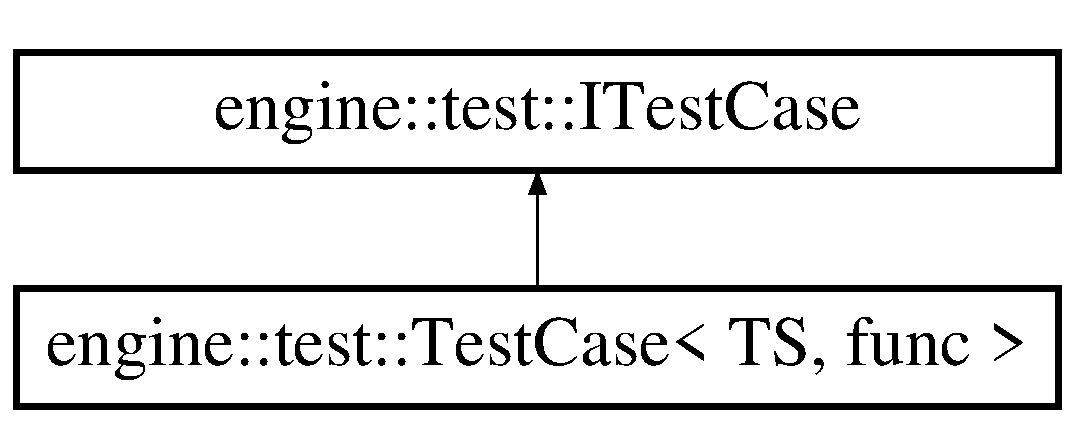
\includegraphics[height=2.000000cm]{a00075}
\end{center}
\end{figure}
\subsubsection*{Public Member Functions}
\begin{DoxyCompactItemize}
\item 
{\bfseries Test\+Case} (TS $\ast$test\+Suite, const std\+::string \&name)\hypertarget{a00075_a0a575a70c45c2096fcd1841e9755d025}{}\label{a00075_a0a575a70c45c2096fcd1841e9755d025}

\item 
void {\bfseries execute} () override\hypertarget{a00075_a2c6d3dc87bef42f18ea52eddb9546566}{}\label{a00075_a2c6d3dc87bef42f18ea52eddb9546566}

\item 
const std\+::string \& {\bfseries get\+Name} () const  override\hypertarget{a00075_a56151c7a0d3e5b1103654cac3dd2b6d0}{}\label{a00075_a56151c7a0d3e5b1103654cac3dd2b6d0}

\end{DoxyCompactItemize}


\subsubsection{Detailed Description}
\subsubsection*{template$<$class TS, void(\+T\+S\+::$\ast$)() func$>$\\*
class engine\+::test\+::\+Test\+Case$<$ T\+S, func $>$}



Definition at line 13 of file Test\+Case.\+h.



The documentation for this class was generated from the following file\+:\begin{DoxyCompactItemize}
\item 
E\+:/\+Programing/\+Projects/\+Engine\+Workspace/\+Common\+Libs/engine/include/engine/test/Test\+Case.\+h\end{DoxyCompactItemize}

\hypertarget{a00076}{}\subsection{engine\+:\+:test\+:\+:Test\+Manager Class Reference}
\label{a00076}\index{engine\+::test\+::\+Test\+Manager@{engine\+::test\+::\+Test\+Manager}}
Inheritance diagram for engine\+:\+:test\+:\+:Test\+Manager\+:\begin{figure}[H]
\begin{center}
\leavevmode
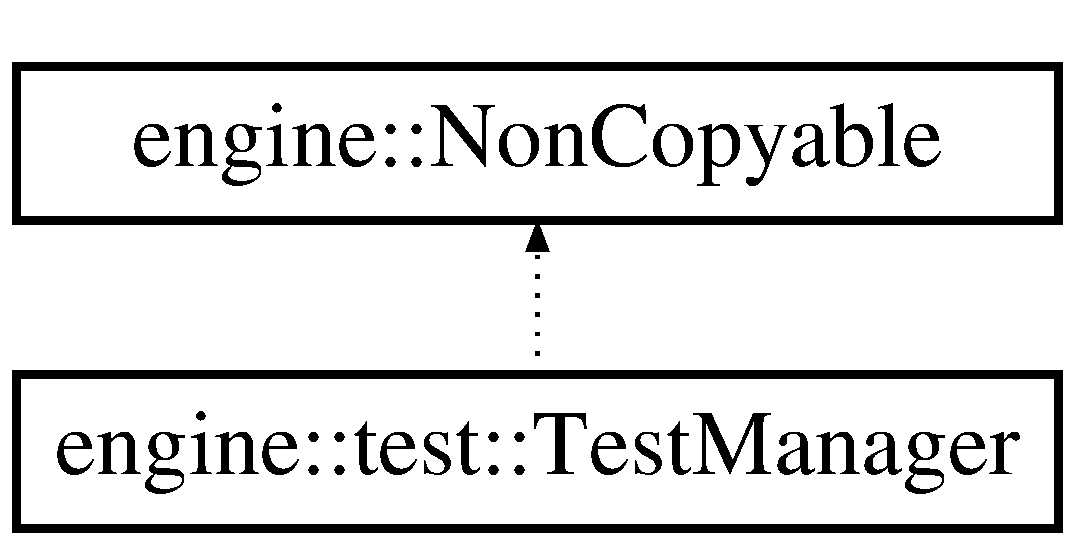
\includegraphics[height=2.000000cm]{a00076}
\end{center}
\end{figure}
\subsubsection*{Public Member Functions}
\begin{DoxyCompactItemize}
\item 
{\bfseries Test\+Manager} (\hyperlink{a00076}{Test\+Manager} \&\&)\hypertarget{a00076_a1fad10153989c4d6a53986abcb638609}{}\label{a00076_a1fad10153989c4d6a53986abcb638609}

\item 
\hyperlink{a00076}{Test\+Manager} \& {\bfseries operator=} (\hyperlink{a00076}{Test\+Manager} \&\&)\hypertarget{a00076_af3d61f894ab863a0da862c3389da4ec8}{}\label{a00076_af3d61f894ab863a0da862c3389da4ec8}

\item 
void {\bfseries add\+Regression} (\hyperlink{a00006}{Base\+Regression} \&\&regression)\hypertarget{a00076_abfffd17a9a11b7eeea95b7b9d1a74b87}{}\label{a00076_abfffd17a9a11b7eeea95b7b9d1a74b87}

\item 
void {\bfseries set\+Output} (std\+::ostream \&os)\hypertarget{a00076_a5a4b820c91787876c3d0b5ec5d4263d9}{}\label{a00076_a5a4b820c91787876c3d0b5ec5d4263d9}

\item 
void {\bfseries run} ()\hypertarget{a00076_abad9d9606204fb93bbe9d5d88c0df755}{}\label{a00076_abad9d9606204fb93bbe9d5d88c0df755}

\end{DoxyCompactItemize}


\subsubsection{Detailed Description}


Definition at line 11 of file Test\+Manager.\+h.



The documentation for this class was generated from the following file\+:\begin{DoxyCompactItemize}
\item 
E\+:/\+Programing/\+Projects/\+Engine\+Workspace/\+Common\+Libs/engine/include/engine/test/Test\+Manager.\+h\end{DoxyCompactItemize}

\hypertarget{a00077}{}\subsection{engine\+:\+:test\+:\+:Test\+Suite Class Reference}
\label{a00077}\index{engine\+::test\+::\+Test\+Suite@{engine\+::test\+::\+Test\+Suite}}
\subsubsection*{Public Member Functions}
\begin{DoxyCompactItemize}
\item 
void {\bfseries add\+Test\+Case} (\hyperlink{a00054}{I\+Test\+Case} $\ast$test\+Case)\hypertarget{a00077_acd67d04d098732ecbbb004baa47cada3}{}\label{a00077_acd67d04d098732ecbbb004baa47cada3}

\item 
void {\bfseries run} () const \hypertarget{a00077_a960f84ba5a59d617afbf780925badfc9}{}\label{a00077_a960f84ba5a59d617afbf780925badfc9}

\item 
void {\bfseries set\+Stream} (std\+::ostream $\ast$os)\hypertarget{a00077_a015fb4b5ed8291b5bd080747234250a5}{}\label{a00077_a015fb4b5ed8291b5bd080747234250a5}

\item 
uint32\+\_\+t {\bfseries get\+Num\+Of\+Nok} () const \hypertarget{a00077_a3cbb7c01265e80c47aa492b58409e08f}{}\label{a00077_a3cbb7c01265e80c47aa492b58409e08f}

\item 
uint32\+\_\+t {\bfseries get\+Num\+Of\+Test\+Cases} () const \hypertarget{a00077_a84e95ee86987b0b4b0c443ecc487edaf}{}\label{a00077_a84e95ee86987b0b4b0c443ecc487edaf}

\item 
float {\bfseries get\+Percentage\+Result} () const \hypertarget{a00077_a7e01d7ba4edd6f30d641b1315fbbb471}{}\label{a00077_a7e01d7ba4edd6f30d641b1315fbbb471}

\end{DoxyCompactItemize}
\subsubsection*{Static Public Attributes}
\begin{DoxyCompactItemize}
\item 
static const size\+\_\+t {\bfseries line\+Length}\hypertarget{a00077_a968656c029005f67f71efa22edbc7689}{}\label{a00077_a968656c029005f67f71efa22edbc7689}

\end{DoxyCompactItemize}
\subsubsection*{Protected Member Functions}
\begin{DoxyCompactItemize}
\item 
{\bfseries Test\+Suite} (const std\+::string \&name)\hypertarget{a00077_a87f9bfcf72c5c5770860ed6504a72c7b}{}\label{a00077_a87f9bfcf72c5c5770860ed6504a72c7b}

\item 
{\bfseries Test\+Suite} (const \hyperlink{a00077}{Test\+Suite} \&o)\hypertarget{a00077_acacadd979ff275c4c2cd66e4786e5300}{}\label{a00077_acacadd979ff275c4c2cd66e4786e5300}

\item 
{\bfseries Test\+Suite} (\hyperlink{a00077}{Test\+Suite} \&\&o)\hypertarget{a00077_a3b26dd3326cf4e5e9c68807990d61570}{}\label{a00077_a3b26dd3326cf4e5e9c68807990d61570}

\item 
void {\bfseries assert\+True} (bool value, const std\+::string \&message, const std\+::string \&file, const uint32\+\_\+t line)\hypertarget{a00077_ac6deffc64b385afc96461903bcd134c7}{}\label{a00077_ac6deffc64b385afc96461903bcd134c7}

\end{DoxyCompactItemize}


\subsubsection{Detailed Description}


Definition at line 9 of file Test\+Suite.\+h.



The documentation for this class was generated from the following file\+:\begin{DoxyCompactItemize}
\item 
E\+:/\+Programing/\+Projects/\+Engine\+Workspace/\+Common\+Libs/engine/include/engine/test/Test\+Suite.\+h\end{DoxyCompactItemize}

\hypertarget{a00078}{}\subsection{engine\+:\+:Unsupported\+Feature Struct Reference}
\label{a00078}\index{engine\+::\+Unsupported\+Feature@{engine\+::\+Unsupported\+Feature}}
Inheritance diagram for engine\+:\+:Unsupported\+Feature\+:\begin{figure}[H]
\begin{center}
\leavevmode
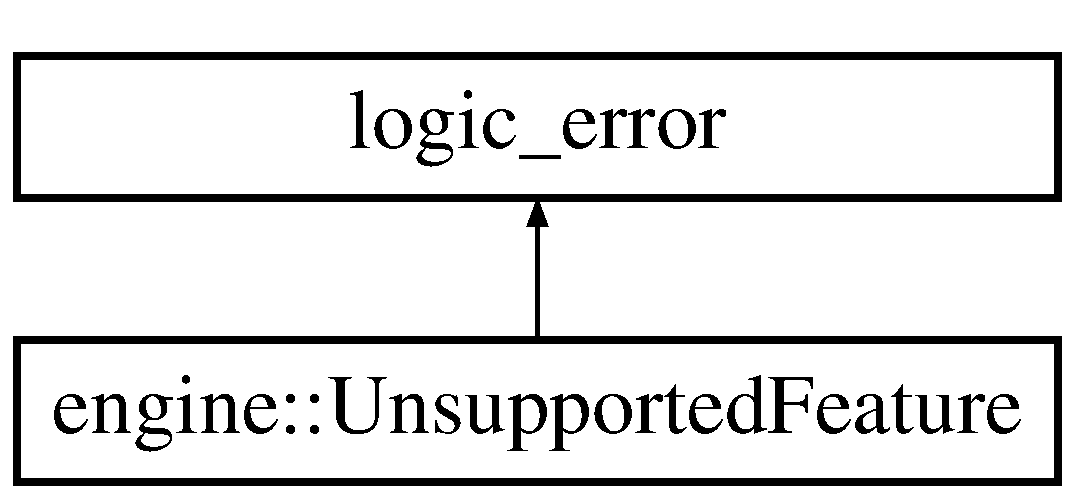
\includegraphics[height=2.000000cm]{a00078}
\end{center}
\end{figure}
\subsubsection*{Public Member Functions}
\begin{DoxyCompactItemize}
\item 
{\bfseries Unsupported\+Feature} (const std\+::string \&error)\hypertarget{a00078_adf506e7a80acd5615803065c18b55b8d}{}\label{a00078_adf506e7a80acd5615803065c18b55b8d}

\item 
{\bfseries Unsupported\+Feature} (const char $\ast$error)\hypertarget{a00078_a0774b1ed4a1653d17c14053dc87e427e}{}\label{a00078_a0774b1ed4a1653d17c14053dc87e427e}

\end{DoxyCompactItemize}


\subsubsection{Detailed Description}


Definition at line 29 of file Logical\+Errors.\+h.



The documentation for this struct was generated from the following file\+:\begin{DoxyCompactItemize}
\item 
E\+:/\+Programing/\+Projects/\+Engine\+Workspace/\+Common\+Libs/engine/include/engine/exceptions/Logical\+Errors.\+h\end{DoxyCompactItemize}

\hypertarget{a00079}{}\subsection{engine\+:\+:Version\+Base$<$ Version\+Class $>$ Class Template Reference}
\label{a00079}\index{engine\+::\+Version\+Base$<$ Version\+Class $>$@{engine\+::\+Version\+Base$<$ Version\+Class $>$}}


{\ttfamily \#include $<$E\+:/\+Programing/\+Projects/\+Engine\+Workspace/\+Common\+Libs/engine/include/engine/utils/\+Version\+Base.\+h$>$}

Inheritance diagram for engine\+:\+:Version\+Base$<$ Version\+Class $>$\+:\begin{figure}[H]
\begin{center}
\leavevmode
\includegraphics[height=1.800643cm]{a00079}
\end{center}
\end{figure}
\subsubsection*{Public Member Functions}
\begin{DoxyCompactItemize}
\item 
int32\+\_\+t \hyperlink{a00079_a87db56a6b48379927ea2c34053ad11d8}{get\+Major} () const 
\item 
int32\+\_\+t \hyperlink{a00079_a9e3c537a417ce0bfbcc6758ad5ae5cb5}{get\+Minor} () const 
\item 
int32\+\_\+t \hyperlink{a00079_a22329ec00668f53aaf4a4efc68d49f93}{get\+Counter} () const 
\item 
int32\+\_\+t \hyperlink{a00079_af8f407400b6b4994c1cd3b243ef84b05}{get\+Year} () const 
\item 
int32\+\_\+t \hyperlink{a00079_a4a3f44823b8caa24943a954385184de2}{get\+Month} () const 
\item 
int32\+\_\+t \hyperlink{a00079_a05c80a133cb8aa10d1c18088f163c206}{get\+Day} () const 
\item 
std\+::string \hyperlink{a00079_aa0b506e6d23023c3efd3a312a39a336d}{get\+String} () const 
\item 
{\footnotesize template$<$class O\+Version\+Class $>$ }\\bool \hyperlink{a00079_a92759ed17bf0e3976ba1bf846b7e21c9}{operator$<$} (const \hyperlink{a00079}{Version\+Base}$<$ O\+Version\+Class $>$ \&o) const 
\item 
{\footnotesize template$<$class O\+Version\+Class $>$ }\\bool \hyperlink{a00079_a4225f1bc4cbcf482bfe688cf0a60fc21}{operator==} (const \hyperlink{a00079}{Version\+Base}$<$ O\+Version\+Class $>$ \&o) const 
\item 
{\footnotesize template$<$class O\+Version\+Class $>$ }\\bool \hyperlink{a00079_a4bff2ae98a2d5883e6dbab5833a51cd7}{operator$>$} (const \hyperlink{a00079}{Version\+Base}$<$ O\+Version\+Class $>$ \&o) const 
\item 
{\footnotesize template$<$class O\+Version\+Class $>$ }\\bool \hyperlink{a00079_a564b9166e177e8657f87f19447aea0cf}{operator$>$=} (const \hyperlink{a00079}{Version\+Base}$<$ O\+Version\+Class $>$ \&o) const 
\item 
{\footnotesize template$<$class O\+Version\+Class $>$ }\\bool \hyperlink{a00079_abd9cbd90f53ff3b5304588349c1b4b7c}{operator$<$=} (const \hyperlink{a00079}{Version\+Base}$<$ O\+Version\+Class $>$ \&o) const 
\item 
{\footnotesize template$<$class O\+Version\+Class $>$ }\\bool \hyperlink{a00079_a87adeb21177fa070dd7fc6a9ffbda5b2}{operator!=} (const \hyperlink{a00079}{Version\+Base}$<$ O\+Version\+Class $>$ \&o) const 
\end{DoxyCompactItemize}
\subsubsection*{Static Public Member Functions}
\begin{DoxyCompactItemize}
\item 
static \hyperlink{a00079}{Version\+Base}$<$ Version\+Class $>$ $\ast$ \hyperlink{a00069_a90ed1f21b1811a569eafccc78fcd12ca}{get\+Instance} ()
\item 
static void \hyperlink{a00069_a571e434c8ff771bf65de40f8a7b22076}{create\+Instance} (Args...\+args)
\item 
static void \hyperlink{a00069_a3fbed1f6a78cdf1d0c11467a3be61841}{release\+Instance} ()
\end{DoxyCompactItemize}
\subsubsection*{Protected Member Functions}
\begin{DoxyCompactItemize}
\item 
\hyperlink{a00079_a706934249d82028c323d45749a13d884}{Version\+Base} ()=default
\end{DoxyCompactItemize}
\subsubsection*{Friends}
\begin{DoxyCompactItemize}
\item 
class {\bfseries Singleton$<$ Version\+Base$<$ Version\+Class $>$ $>$}\hypertarget{a00079_a1c46032cef993c3af14bd8a1ddf00716}{}\label{a00079_a1c46032cef993c3af14bd8a1ddf00716}

\end{DoxyCompactItemize}


\subsubsection{Detailed Description}
\subsubsection*{template$<$class Version\+Class$>$\\*
class engine\+::\+Version\+Base$<$ Version\+Class $>$}

Template base class to extend version classes. 
\begin{DoxyTemplParams}{Template Parameters}
{\em Version\+Class} & The class to extend functionalities. \\
\hline
\end{DoxyTemplParams}


Definition at line 12 of file Version\+Base.\+h.



\subsubsection{Constructor \& Destructor Documentation}
\index{engine\+::\+Version\+Base@{engine\+::\+Version\+Base}!Version\+Base@{Version\+Base}}
\index{Version\+Base@{Version\+Base}!engine\+::\+Version\+Base@{engine\+::\+Version\+Base}}
\paragraph[{\texorpdfstring{Version\+Base()=default}{VersionBase()=default}}]{\setlength{\rightskip}{0pt plus 5cm}template$<$class Version\+Class$>$ {\bf engine\+::\+Version\+Base}$<$ Version\+Class $>$\+::{\bf Version\+Base} (
\begin{DoxyParamCaption}
{}
\end{DoxyParamCaption}
)\hspace{0.3cm}{\ttfamily [protected]}, {\ttfamily [default]}}\hypertarget{a00079_a706934249d82028c323d45749a13d884}{}\label{a00079_a706934249d82028c323d45749a13d884}
Defualt constructable 

\subsubsection{Member Function Documentation}
\index{engine\+::\+Version\+Base@{engine\+::\+Version\+Base}!create\+Instance@{create\+Instance}}
\index{create\+Instance@{create\+Instance}!engine\+::\+Version\+Base@{engine\+::\+Version\+Base}}
\paragraph[{\texorpdfstring{create\+Instance(\+Args...\+args)}{createInstance(Args...args)}}]{\setlength{\rightskip}{0pt plus 5cm}static void {\bf engine\+::\+Singleton}$<$ {\bf Version\+Base}$<$ Version\+Class $>$  $>$\+::create\+Instance (
\begin{DoxyParamCaption}
\item[{Args...}]{args}
\end{DoxyParamCaption}
)\hspace{0.3cm}{\ttfamily [static]}, {\ttfamily [inherited]}}\hypertarget{a00069_a571e434c8ff771bf65de40f8a7b22076}{}\label{a00069_a571e434c8ff771bf65de40f8a7b22076}
Create an instance with the given arguments 
\begin{DoxyParams}{Parameters}
{\em creation} & arguments \\
\hline
\end{DoxyParams}
\index{engine\+::\+Version\+Base@{engine\+::\+Version\+Base}!get\+Counter@{get\+Counter}}
\index{get\+Counter@{get\+Counter}!engine\+::\+Version\+Base@{engine\+::\+Version\+Base}}
\paragraph[{\texorpdfstring{get\+Counter() const }{getCounter() const }}]{\setlength{\rightskip}{0pt plus 5cm}template$<$class Version\+Class$>$ int32\+\_\+t {\bf engine\+::\+Version\+Base}$<$ Version\+Class $>$\+::get\+Counter (
\begin{DoxyParamCaption}
{}
\end{DoxyParamCaption}
) const}\hypertarget{a00079_a22329ec00668f53aaf4a4efc68d49f93}{}\label{a00079_a22329ec00668f53aaf4a4efc68d49f93}
\begin{DoxyReturn}{Returns}
Returns the counter part 
\end{DoxyReturn}
\index{engine\+::\+Version\+Base@{engine\+::\+Version\+Base}!get\+Day@{get\+Day}}
\index{get\+Day@{get\+Day}!engine\+::\+Version\+Base@{engine\+::\+Version\+Base}}
\paragraph[{\texorpdfstring{get\+Day() const }{getDay() const }}]{\setlength{\rightskip}{0pt plus 5cm}template$<$class Version\+Class$>$ int32\+\_\+t {\bf engine\+::\+Version\+Base}$<$ Version\+Class $>$\+::get\+Day (
\begin{DoxyParamCaption}
{}
\end{DoxyParamCaption}
) const}\hypertarget{a00079_a05c80a133cb8aa10d1c18088f163c206}{}\label{a00079_a05c80a133cb8aa10d1c18088f163c206}
\begin{DoxyReturn}{Returns}
Returns the build day 
\end{DoxyReturn}
\index{engine\+::\+Version\+Base@{engine\+::\+Version\+Base}!get\+Instance@{get\+Instance}}
\index{get\+Instance@{get\+Instance}!engine\+::\+Version\+Base@{engine\+::\+Version\+Base}}
\paragraph[{\texorpdfstring{get\+Instance()}{getInstance()}}]{\setlength{\rightskip}{0pt plus 5cm}static {\bf Version\+Base}$<$ Version\+Class $>$ $\ast$ {\bf engine\+::\+Singleton}$<$ {\bf Version\+Base}$<$ Version\+Class $>$  $>$\+::get\+Instance (
\begin{DoxyParamCaption}
{}
\end{DoxyParamCaption}
)\hspace{0.3cm}{\ttfamily [static]}, {\ttfamily [inherited]}}\hypertarget{a00069_a90ed1f21b1811a569eafccc78fcd12ca}{}\label{a00069_a90ed1f21b1811a569eafccc78fcd12ca}
\begin{DoxyReturn}{Returns}
the instance object 
\end{DoxyReturn}
\index{engine\+::\+Version\+Base@{engine\+::\+Version\+Base}!get\+Major@{get\+Major}}
\index{get\+Major@{get\+Major}!engine\+::\+Version\+Base@{engine\+::\+Version\+Base}}
\paragraph[{\texorpdfstring{get\+Major() const }{getMajor() const }}]{\setlength{\rightskip}{0pt plus 5cm}template$<$class Version\+Class$>$ int32\+\_\+t {\bf engine\+::\+Version\+Base}$<$ Version\+Class $>$\+::get\+Major (
\begin{DoxyParamCaption}
{}
\end{DoxyParamCaption}
) const}\hypertarget{a00079_a87db56a6b48379927ea2c34053ad11d8}{}\label{a00079_a87db56a6b48379927ea2c34053ad11d8}
\begin{DoxyReturn}{Returns}
Returns the major number 
\end{DoxyReturn}
\index{engine\+::\+Version\+Base@{engine\+::\+Version\+Base}!get\+Minor@{get\+Minor}}
\index{get\+Minor@{get\+Minor}!engine\+::\+Version\+Base@{engine\+::\+Version\+Base}}
\paragraph[{\texorpdfstring{get\+Minor() const }{getMinor() const }}]{\setlength{\rightskip}{0pt plus 5cm}template$<$class Version\+Class$>$ int32\+\_\+t {\bf engine\+::\+Version\+Base}$<$ Version\+Class $>$\+::get\+Minor (
\begin{DoxyParamCaption}
{}
\end{DoxyParamCaption}
) const}\hypertarget{a00079_a9e3c537a417ce0bfbcc6758ad5ae5cb5}{}\label{a00079_a9e3c537a417ce0bfbcc6758ad5ae5cb5}
\begin{DoxyReturn}{Returns}
Returns the minor number 
\end{DoxyReturn}
\index{engine\+::\+Version\+Base@{engine\+::\+Version\+Base}!get\+Month@{get\+Month}}
\index{get\+Month@{get\+Month}!engine\+::\+Version\+Base@{engine\+::\+Version\+Base}}
\paragraph[{\texorpdfstring{get\+Month() const }{getMonth() const }}]{\setlength{\rightskip}{0pt plus 5cm}template$<$class Version\+Class$>$ int32\+\_\+t {\bf engine\+::\+Version\+Base}$<$ Version\+Class $>$\+::get\+Month (
\begin{DoxyParamCaption}
{}
\end{DoxyParamCaption}
) const}\hypertarget{a00079_a4a3f44823b8caa24943a954385184de2}{}\label{a00079_a4a3f44823b8caa24943a954385184de2}
\begin{DoxyReturn}{Returns}
Returns the build month 
\end{DoxyReturn}
\index{engine\+::\+Version\+Base@{engine\+::\+Version\+Base}!get\+String@{get\+String}}
\index{get\+String@{get\+String}!engine\+::\+Version\+Base@{engine\+::\+Version\+Base}}
\paragraph[{\texorpdfstring{get\+String() const }{getString() const }}]{\setlength{\rightskip}{0pt plus 5cm}template$<$class Version\+Class$>$ std\+::string {\bf engine\+::\+Version\+Base}$<$ Version\+Class $>$\+::get\+String (
\begin{DoxyParamCaption}
{}
\end{DoxyParamCaption}
) const}\hypertarget{a00079_aa0b506e6d23023c3efd3a312a39a336d}{}\label{a00079_aa0b506e6d23023c3efd3a312a39a336d}
\begin{DoxyReturn}{Returns}
Returns the string format 
\end{DoxyReturn}
\index{engine\+::\+Version\+Base@{engine\+::\+Version\+Base}!get\+Year@{get\+Year}}
\index{get\+Year@{get\+Year}!engine\+::\+Version\+Base@{engine\+::\+Version\+Base}}
\paragraph[{\texorpdfstring{get\+Year() const }{getYear() const }}]{\setlength{\rightskip}{0pt plus 5cm}template$<$class Version\+Class$>$ int32\+\_\+t {\bf engine\+::\+Version\+Base}$<$ Version\+Class $>$\+::get\+Year (
\begin{DoxyParamCaption}
{}
\end{DoxyParamCaption}
) const}\hypertarget{a00079_af8f407400b6b4994c1cd3b243ef84b05}{}\label{a00079_af8f407400b6b4994c1cd3b243ef84b05}
\begin{DoxyReturn}{Returns}
Returns the build year 
\end{DoxyReturn}
\index{engine\+::\+Version\+Base@{engine\+::\+Version\+Base}!operator"!=@{operator"!=}}
\index{operator"!=@{operator"!=}!engine\+::\+Version\+Base@{engine\+::\+Version\+Base}}
\paragraph[{\texorpdfstring{operator"!=(const Version\+Base$<$ O\+Version\+Class $>$ \&o) const }{operator!=(const VersionBase< OVersionClass > &o) const }}]{\setlength{\rightskip}{0pt plus 5cm}template$<$class Version\+Class$>$ template$<$class O\+Version\+Class $>$ bool {\bf engine\+::\+Version\+Base}$<$ Version\+Class $>$\+::operator!= (
\begin{DoxyParamCaption}
\item[{const {\bf Version\+Base}$<$ O\+Version\+Class $>$ \&}]{o}
\end{DoxyParamCaption}
) const}\hypertarget{a00079_a87adeb21177fa070dd7fc6a9ffbda5b2}{}\label{a00079_a87adeb21177fa070dd7fc6a9ffbda5b2}
Comparson operator. 
\begin{DoxyParams}{Parameters}
{\em o} & other object \\
\hline
\end{DoxyParams}
\index{engine\+::\+Version\+Base@{engine\+::\+Version\+Base}!operator$<$@{operator$<$}}
\index{operator$<$@{operator$<$}!engine\+::\+Version\+Base@{engine\+::\+Version\+Base}}
\paragraph[{\texorpdfstring{operator$<$(const Version\+Base$<$ O\+Version\+Class $>$ \&o) const }{operator<(const VersionBase< OVersionClass > &o) const }}]{\setlength{\rightskip}{0pt plus 5cm}template$<$class Version\+Class$>$ template$<$class O\+Version\+Class $>$ bool {\bf engine\+::\+Version\+Base}$<$ Version\+Class $>$\+::operator$<$ (
\begin{DoxyParamCaption}
\item[{const {\bf Version\+Base}$<$ O\+Version\+Class $>$ \&}]{o}
\end{DoxyParamCaption}
) const}\hypertarget{a00079_a92759ed17bf0e3976ba1bf846b7e21c9}{}\label{a00079_a92759ed17bf0e3976ba1bf846b7e21c9}
Comparson operator. 
\begin{DoxyParams}{Parameters}
{\em o} & other object \\
\hline
\end{DoxyParams}
\index{engine\+::\+Version\+Base@{engine\+::\+Version\+Base}!operator$<$=@{operator$<$=}}
\index{operator$<$=@{operator$<$=}!engine\+::\+Version\+Base@{engine\+::\+Version\+Base}}
\paragraph[{\texorpdfstring{operator$<$=(const Version\+Base$<$ O\+Version\+Class $>$ \&o) const }{operator<=(const VersionBase< OVersionClass > &o) const }}]{\setlength{\rightskip}{0pt plus 5cm}template$<$class Version\+Class$>$ template$<$class O\+Version\+Class $>$ bool {\bf engine\+::\+Version\+Base}$<$ Version\+Class $>$\+::operator$<$= (
\begin{DoxyParamCaption}
\item[{const {\bf Version\+Base}$<$ O\+Version\+Class $>$ \&}]{o}
\end{DoxyParamCaption}
) const}\hypertarget{a00079_abd9cbd90f53ff3b5304588349c1b4b7c}{}\label{a00079_abd9cbd90f53ff3b5304588349c1b4b7c}
Comparson operator. 
\begin{DoxyParams}{Parameters}
{\em o} & other object \\
\hline
\end{DoxyParams}
\index{engine\+::\+Version\+Base@{engine\+::\+Version\+Base}!operator==@{operator==}}
\index{operator==@{operator==}!engine\+::\+Version\+Base@{engine\+::\+Version\+Base}}
\paragraph[{\texorpdfstring{operator==(const Version\+Base$<$ O\+Version\+Class $>$ \&o) const }{operator==(const VersionBase< OVersionClass > &o) const }}]{\setlength{\rightskip}{0pt plus 5cm}template$<$class Version\+Class$>$ template$<$class O\+Version\+Class $>$ bool {\bf engine\+::\+Version\+Base}$<$ Version\+Class $>$\+::operator== (
\begin{DoxyParamCaption}
\item[{const {\bf Version\+Base}$<$ O\+Version\+Class $>$ \&}]{o}
\end{DoxyParamCaption}
) const}\hypertarget{a00079_a4225f1bc4cbcf482bfe688cf0a60fc21}{}\label{a00079_a4225f1bc4cbcf482bfe688cf0a60fc21}
Comparson operator. 
\begin{DoxyParams}{Parameters}
{\em o} & other object \\
\hline
\end{DoxyParams}
\index{engine\+::\+Version\+Base@{engine\+::\+Version\+Base}!operator$>$@{operator$>$}}
\index{operator$>$@{operator$>$}!engine\+::\+Version\+Base@{engine\+::\+Version\+Base}}
\paragraph[{\texorpdfstring{operator$>$(const Version\+Base$<$ O\+Version\+Class $>$ \&o) const }{operator>(const VersionBase< OVersionClass > &o) const }}]{\setlength{\rightskip}{0pt plus 5cm}template$<$class Version\+Class$>$ template$<$class O\+Version\+Class $>$ bool {\bf engine\+::\+Version\+Base}$<$ Version\+Class $>$\+::operator$>$ (
\begin{DoxyParamCaption}
\item[{const {\bf Version\+Base}$<$ O\+Version\+Class $>$ \&}]{o}
\end{DoxyParamCaption}
) const}\hypertarget{a00079_a4bff2ae98a2d5883e6dbab5833a51cd7}{}\label{a00079_a4bff2ae98a2d5883e6dbab5833a51cd7}
Comparson operator. 
\begin{DoxyParams}{Parameters}
{\em o} & other object \\
\hline
\end{DoxyParams}
\index{engine\+::\+Version\+Base@{engine\+::\+Version\+Base}!operator$>$=@{operator$>$=}}
\index{operator$>$=@{operator$>$=}!engine\+::\+Version\+Base@{engine\+::\+Version\+Base}}
\paragraph[{\texorpdfstring{operator$>$=(const Version\+Base$<$ O\+Version\+Class $>$ \&o) const }{operator>=(const VersionBase< OVersionClass > &o) const }}]{\setlength{\rightskip}{0pt plus 5cm}template$<$class Version\+Class$>$ template$<$class O\+Version\+Class $>$ bool {\bf engine\+::\+Version\+Base}$<$ Version\+Class $>$\+::operator$>$= (
\begin{DoxyParamCaption}
\item[{const {\bf Version\+Base}$<$ O\+Version\+Class $>$ \&}]{o}
\end{DoxyParamCaption}
) const}\hypertarget{a00079_a564b9166e177e8657f87f19447aea0cf}{}\label{a00079_a564b9166e177e8657f87f19447aea0cf}
Comparson operator. 
\begin{DoxyParams}{Parameters}
{\em o} & other object \\
\hline
\end{DoxyParams}
\index{engine\+::\+Version\+Base@{engine\+::\+Version\+Base}!release\+Instance@{release\+Instance}}
\index{release\+Instance@{release\+Instance}!engine\+::\+Version\+Base@{engine\+::\+Version\+Base}}
\paragraph[{\texorpdfstring{release\+Instance()}{releaseInstance()}}]{\setlength{\rightskip}{0pt plus 5cm}static void {\bf engine\+::\+Singleton}$<$ {\bf Version\+Base}$<$ Version\+Class $>$  $>$\+::release\+Instance (
\begin{DoxyParamCaption}
{}
\end{DoxyParamCaption}
)\hspace{0.3cm}{\ttfamily [static]}, {\ttfamily [inherited]}}\hypertarget{a00069_a3fbed1f6a78cdf1d0c11467a3be61841}{}\label{a00069_a3fbed1f6a78cdf1d0c11467a3be61841}
Delete the instance 

The documentation for this class was generated from the following file\+:\begin{DoxyCompactItemize}
\item 
E\+:/\+Programing/\+Projects/\+Engine\+Workspace/\+Common\+Libs/engine/include/engine/utils/Version\+Base.\+h\end{DoxyCompactItemize}

\hypertarget{a00080}{}\subsection{engine\+:\+:version\+:\+:Version\+Def Class Reference}
\label{a00080}\index{engine\+::version\+::\+Version\+Def@{engine\+::version\+::\+Version\+Def}}
\subsubsection*{Protected Attributes}
\begin{DoxyCompactItemize}
\item 
const int {\bfseries major} = 0\hypertarget{a00080_a0b9a44d65bbc763dcd74daf581572fe2}{}\label{a00080_a0b9a44d65bbc763dcd74daf581572fe2}

\item 
const int {\bfseries minor} = 1\hypertarget{a00080_a677bfac625f58b5804d70f14861eb26e}{}\label{a00080_a677bfac625f58b5804d70f14861eb26e}

\item 
const int {\bfseries counter} = 1\hypertarget{a00080_aba60198eae9769727969c909073c7a7d}{}\label{a00080_aba60198eae9769727969c909073c7a7d}

\item 
const std\+::string {\bfseries year} = \char`\"{}17\char`\"{}\hypertarget{a00080_aa546ca8748276eccf7ab3b616eb8bed3}{}\label{a00080_aa546ca8748276eccf7ab3b616eb8bed3}

\item 
const std\+::string {\bfseries month} = \char`\"{}03\char`\"{}\hypertarget{a00080_aeea4822a81d2dd44c4d23c224f6504c6}{}\label{a00080_aeea4822a81d2dd44c4d23c224f6504c6}

\item 
const std\+::string {\bfseries day} = \char`\"{}30\char`\"{}\hypertarget{a00080_a141d3e9a073994719672fc21cb251627}{}\label{a00080_a141d3e9a073994719672fc21cb251627}

\end{DoxyCompactItemize}


\subsubsection{Detailed Description}


Definition at line 9 of file Engine\+Config.\+h.



The documentation for this class was generated from the following file\+:\begin{DoxyCompactItemize}
\item 
E\+:/\+Programing/\+Projects/\+Engine\+Workspace/\+Common\+Libs/engine/include/engine/Engine\+Config.\+h\end{DoxyCompactItemize}

\hypertarget{a00081}{}\subsection{engine\+:\+:winapi\+:\+:Win\+Api\+Application\+Parameter Class Reference}
\label{a00081}\index{engine\+::winapi\+::\+Win\+Api\+Application\+Parameter@{engine\+::winapi\+::\+Win\+Api\+Application\+Parameter}}


{\ttfamily \#include $<$E\+:/\+Programing/\+Projects/\+Engine\+Workspace/\+Common\+Libs/engine/include/engine/app/winapi/\+Win\+Api\+Application\+Parameter.\+h$>$}

Inheritance diagram for engine\+:\+:winapi\+:\+:Win\+Api\+Application\+Parameter\+:\begin{figure}[H]
\begin{center}
\leavevmode
\includegraphics[height=3.000000cm]{a00081}
\end{center}
\end{figure}
\subsubsection*{Public Member Functions}
\begin{DoxyCompactItemize}
\item 
\hyperlink{a00081_af7fef7fdba7239b1b01e9ba9c46c1a32}{Win\+Api\+Application\+Parameter} (H\+I\+N\+S\+T\+A\+N\+CE instance, H\+I\+N\+S\+T\+A\+N\+CE prev\+Instance, L\+P\+S\+TR cmd\+Line, int cmd\+Show)
\item 
\hyperlink{a00081_a8cf7f2740093b195aa980b9791b2b4cb}{$\sim$\+Win\+Api\+Application\+Parameter} () override
\item 
H\+I\+N\+S\+T\+A\+N\+CE \hyperlink{a00081_a35f806d57b22fa9bcab1b6391a8060b7}{get\+Instance} () const 
\item 
int \hyperlink{a00081_a30232e7cd9fce28ce65b7b3b7325f69f}{get\+Cmd\+Show} () const 
\item 
const std\+::vector$<$ std\+::string $>$ \& \hyperlink{a00071_ae482854d2439758cfd1d2c710c621b4f}{get\+Parameters} () const 
\item 
const std\+::string \& \hyperlink{a00071_a5d29ea3dfb725dc1a386926896b5a48a}{get\+Binary\+Name} () const 
\end{DoxyCompactItemize}
\subsubsection*{Protected Member Functions}
\begin{DoxyCompactItemize}
\item 
void \hyperlink{a00071_aaf7d27892d7fbad5573099a4fabb6218}{init} (uint32\+\_\+t n\+Params, const std\+::vector$<$ std\+::string $>$ \&parameters)
\end{DoxyCompactItemize}


\subsubsection{Detailed Description}
Win\+Api applications have special parameters. This class is the specialization of standard parameters. 

Definition at line 11 of file Win\+Api\+Application\+Parameter.\+h.



\subsubsection{Constructor \& Destructor Documentation}
\index{engine\+::winapi\+::\+Win\+Api\+Application\+Parameter@{engine\+::winapi\+::\+Win\+Api\+Application\+Parameter}!Win\+Api\+Application\+Parameter@{Win\+Api\+Application\+Parameter}}
\index{Win\+Api\+Application\+Parameter@{Win\+Api\+Application\+Parameter}!engine\+::winapi\+::\+Win\+Api\+Application\+Parameter@{engine\+::winapi\+::\+Win\+Api\+Application\+Parameter}}
\paragraph[{\texorpdfstring{Win\+Api\+Application\+Parameter(\+H\+I\+N\+S\+T\+A\+N\+C\+E instance, H\+I\+N\+S\+T\+A\+N\+C\+E prev\+Instance, L\+P\+S\+T\+R cmd\+Line, int cmd\+Show)}{WinApiApplicationParameter(HINSTANCE instance, HINSTANCE prevInstance, LPSTR cmdLine, int cmdShow)}}]{\setlength{\rightskip}{0pt plus 5cm}engine\+::winapi\+::\+Win\+Api\+Application\+Parameter\+::\+Win\+Api\+Application\+Parameter (
\begin{DoxyParamCaption}
\item[{H\+I\+N\+S\+T\+A\+N\+CE}]{instance, }
\item[{H\+I\+N\+S\+T\+A\+N\+CE}]{prev\+Instance, }
\item[{L\+P\+S\+TR}]{cmd\+Line, }
\item[{int}]{cmd\+Show}
\end{DoxyParamCaption}
)}\hypertarget{a00081_af7fef7fdba7239b1b01e9ba9c46c1a32}{}\label{a00081_af7fef7fdba7239b1b01e9ba9c46c1a32}
Win\+Api application parameter initialization. 
\begin{DoxyParams}{Parameters}
{\em instance} & Handler for the current application instance. \\
\hline
{\em prev\+Instance} & Due to historical reason we got the previous application handler too. \\
\hline
{\em cmd\+Line} & Standard command line arguments except the current application name \\
\hline
{\em cmd\+Show} & flag for window showing. \\
\hline
\end{DoxyParams}
\begin{DoxySeeAlso}{See also}
\href{https://msdn.microsoft.com/en-us/library/windows/desktop/ff381406(v=vs.85).aspx}{\tt https\+://msdn.\+microsoft.\+com/en-\/us/library/windows/desktop/ff381406(v=vs.\+85).\+aspx} 
\end{DoxySeeAlso}
\index{engine\+::winapi\+::\+Win\+Api\+Application\+Parameter@{engine\+::winapi\+::\+Win\+Api\+Application\+Parameter}!````~Win\+Api\+Application\+Parameter@{$\sim$\+Win\+Api\+Application\+Parameter}}
\index{````~Win\+Api\+Application\+Parameter@{$\sim$\+Win\+Api\+Application\+Parameter}!engine\+::winapi\+::\+Win\+Api\+Application\+Parameter@{engine\+::winapi\+::\+Win\+Api\+Application\+Parameter}}
\paragraph[{\texorpdfstring{$\sim$\+Win\+Api\+Application\+Parameter() override}{~WinApiApplicationParameter() override}}]{\setlength{\rightskip}{0pt plus 5cm}engine\+::winapi\+::\+Win\+Api\+Application\+Parameter\+::$\sim$\+Win\+Api\+Application\+Parameter (
\begin{DoxyParamCaption}
{}
\end{DoxyParamCaption}
)\hspace{0.3cm}{\ttfamily [override]}}\hypertarget{a00081_a8cf7f2740093b195aa980b9791b2b4cb}{}\label{a00081_a8cf7f2740093b195aa980b9791b2b4cb}
Destructor for P\+I\+M\+PL 

\subsubsection{Member Function Documentation}
\index{engine\+::winapi\+::\+Win\+Api\+Application\+Parameter@{engine\+::winapi\+::\+Win\+Api\+Application\+Parameter}!get\+Binary\+Name@{get\+Binary\+Name}}
\index{get\+Binary\+Name@{get\+Binary\+Name}!engine\+::winapi\+::\+Win\+Api\+Application\+Parameter@{engine\+::winapi\+::\+Win\+Api\+Application\+Parameter}}
\paragraph[{\texorpdfstring{get\+Binary\+Name() const }{getBinaryName() const }}]{\setlength{\rightskip}{0pt plus 5cm}const std\+::string\& engine\+::\+Standard\+Application\+Parameter\+::get\+Binary\+Name (
\begin{DoxyParamCaption}
{}
\end{DoxyParamCaption}
) const\hspace{0.3cm}{\ttfamily [inherited]}}\hypertarget{a00071_a5d29ea3dfb725dc1a386926896b5a48a}{}\label{a00071_a5d29ea3dfb725dc1a386926896b5a48a}
\begin{DoxyReturn}{Returns}
Returns the name of the binary 
\end{DoxyReturn}
\index{engine\+::winapi\+::\+Win\+Api\+Application\+Parameter@{engine\+::winapi\+::\+Win\+Api\+Application\+Parameter}!get\+Cmd\+Show@{get\+Cmd\+Show}}
\index{get\+Cmd\+Show@{get\+Cmd\+Show}!engine\+::winapi\+::\+Win\+Api\+Application\+Parameter@{engine\+::winapi\+::\+Win\+Api\+Application\+Parameter}}
\paragraph[{\texorpdfstring{get\+Cmd\+Show() const }{getCmdShow() const }}]{\setlength{\rightskip}{0pt plus 5cm}int engine\+::winapi\+::\+Win\+Api\+Application\+Parameter\+::get\+Cmd\+Show (
\begin{DoxyParamCaption}
{}
\end{DoxyParamCaption}
) const}\hypertarget{a00081_a30232e7cd9fce28ce65b7b3b7325f69f}{}\label{a00081_a30232e7cd9fce28ce65b7b3b7325f69f}
\begin{DoxyReturn}{Returns}
Returns the flag for window showing parameter (minimalize/maximize/show normaly) 
\end{DoxyReturn}
\index{engine\+::winapi\+::\+Win\+Api\+Application\+Parameter@{engine\+::winapi\+::\+Win\+Api\+Application\+Parameter}!get\+Instance@{get\+Instance}}
\index{get\+Instance@{get\+Instance}!engine\+::winapi\+::\+Win\+Api\+Application\+Parameter@{engine\+::winapi\+::\+Win\+Api\+Application\+Parameter}}
\paragraph[{\texorpdfstring{get\+Instance() const }{getInstance() const }}]{\setlength{\rightskip}{0pt plus 5cm}H\+I\+N\+S\+T\+A\+N\+CE engine\+::winapi\+::\+Win\+Api\+Application\+Parameter\+::get\+Instance (
\begin{DoxyParamCaption}
{}
\end{DoxyParamCaption}
) const}\hypertarget{a00081_a35f806d57b22fa9bcab1b6391a8060b7}{}\label{a00081_a35f806d57b22fa9bcab1b6391a8060b7}
\begin{DoxyReturn}{Returns}
Returns the handler for the application instance 
\end{DoxyReturn}
\index{engine\+::winapi\+::\+Win\+Api\+Application\+Parameter@{engine\+::winapi\+::\+Win\+Api\+Application\+Parameter}!get\+Parameters@{get\+Parameters}}
\index{get\+Parameters@{get\+Parameters}!engine\+::winapi\+::\+Win\+Api\+Application\+Parameter@{engine\+::winapi\+::\+Win\+Api\+Application\+Parameter}}
\paragraph[{\texorpdfstring{get\+Parameters() const }{getParameters() const }}]{\setlength{\rightskip}{0pt plus 5cm}const std\+::vector$<$std\+::string$>$\& engine\+::\+Standard\+Application\+Parameter\+::get\+Parameters (
\begin{DoxyParamCaption}
{}
\end{DoxyParamCaption}
) const\hspace{0.3cm}{\ttfamily [inherited]}}\hypertarget{a00071_ae482854d2439758cfd1d2c710c621b4f}{}\label{a00071_ae482854d2439758cfd1d2c710c621b4f}
\begin{DoxyReturn}{Returns}
Returns the parameters in a vector 
\end{DoxyReturn}
\index{engine\+::winapi\+::\+Win\+Api\+Application\+Parameter@{engine\+::winapi\+::\+Win\+Api\+Application\+Parameter}!init@{init}}
\index{init@{init}!engine\+::winapi\+::\+Win\+Api\+Application\+Parameter@{engine\+::winapi\+::\+Win\+Api\+Application\+Parameter}}
\paragraph[{\texorpdfstring{init(uint32\+\_\+t n\+Params, const std\+::vector$<$ std\+::string $>$ \&parameters)}{init(uint32_t nParams, const std::vector< std::string > &parameters)}}]{\setlength{\rightskip}{0pt plus 5cm}void engine\+::\+Standard\+Application\+Parameter\+::init (
\begin{DoxyParamCaption}
\item[{uint32\+\_\+t}]{n\+Params, }
\item[{const std\+::vector$<$ std\+::string $>$ \&}]{parameters}
\end{DoxyParamCaption}
)\hspace{0.3cm}{\ttfamily [protected]}, {\ttfamily [inherited]}}\hypertarget{a00071_aaf7d27892d7fbad5573099a4fabb6218}{}\label{a00071_aaf7d27892d7fbad5573099a4fabb6218}
Function for initialize the members 

The documentation for this class was generated from the following file\+:\begin{DoxyCompactItemize}
\item 
E\+:/\+Programing/\+Projects/\+Engine\+Workspace/\+Common\+Libs/engine/include/engine/app/winapi/Win\+Api\+Application\+Parameter.\+h\end{DoxyCompactItemize}

\hypertarget{a00082}{}\subsection{engine\+:\+:Window Class Reference}
\label{a00082}\index{engine\+::\+Window@{engine\+::\+Window}}


{\ttfamily \#include $<$E\+:/\+Programing/\+Projects/\+Engine\+Workspace/\+Common\+Libs/engine/include/engine/view/\+Window.\+h$>$}

Inheritance diagram for engine\+:\+:Window\+:\begin{figure}[H]
\begin{center}
\leavevmode
\includegraphics[height=2.647754cm]{a00082}
\end{center}
\end{figure}
\subsubsection*{Public Member Functions}
\begin{DoxyCompactItemize}
\item 
\hyperlink{a00082_a6adceceb01e5ed546282c5ea2d09af88}{Window} ()
\item 
\hyperlink{a00082_a3bf48ba460f021664ad27f27509cf473}{Window} (const \hyperlink{a00091}{Window\+Parameter} \&parameter)
\item 
virtual \hyperlink{a00082_a9540302516f5eda30facee89517346ed}{$\sim$\+Window} ()
\item 
const \hyperlink{a00091}{Window\+Parameter} \& \hyperlink{a00082_afbb0f8b825f17fbf8f434c4ab9ae5f8d}{get\+Parameters} () const 
\item 
void \hyperlink{a00082_ad6874b68c5cd0b59ec75ac8ad15f2a3a}{set\+Position} (int32\+\_\+t x, int32\+\_\+t y)
\item 
void \hyperlink{a00082_a3435c3bf0e07492ec77f3977c9b5e355}{set\+Width} (uint32\+\_\+t width)
\item 
uint32\+\_\+t {\bfseries get\+Width} () const \hypertarget{a00082_a8f13b82e3aa16ac711b2efd5411964d0}{}\label{a00082_a8f13b82e3aa16ac711b2efd5411964d0}

\item 
void \hyperlink{a00082_a87b8b6f2c1a08327d4010e2b6aceb319}{set\+Height} (uint32\+\_\+t height)
\item 
uint32\+\_\+t {\bfseries get\+Height} () const \hypertarget{a00082_accdce871efc461fe3348d62f8087b73d}{}\label{a00082_accdce871efc461fe3348d62f8087b73d}

\item 
void \hyperlink{a00082_aefaae1015e22521e0a0168633a7d413f}{set\+Size} (uint32\+\_\+t width, uint32\+\_\+t height)
\item 
bool \hyperlink{a00082_a9429ac0c042cc998ecbedb1c13c0bc9a}{is\+Full\+Screen} () const 
\item 
\hyperlink{a00024}{Driver} $\ast$ {\bfseries get\+Driver} () const \hypertarget{a00082_ac793b7cdbbdd1d62df9dc64e4ed50b27}{}\label{a00082_ac793b7cdbbdd1d62df9dc64e4ed50b27}

\item 
void {\bfseries init\+Driver} (std\+::unique\+\_\+ptr$<$ \hyperlink{a00024}{Driver} $>$ driver)\hypertarget{a00082_a23c30f984006bdf0d2ceda4513ee12b9}{}\label{a00082_a23c30f984006bdf0d2ceda4513ee12b9}

\item 
void {\bfseries set\+Events\+Enabled} (bool v)\hypertarget{a00036_ae529242181c16462bef9bd6b8fb56b93}{}\label{a00036_ae529242181c16462bef9bd6b8fb56b93}

\item 
bool {\bfseries is\+Events\+Enabled} () const \hypertarget{a00036_a659325f18d666f132f380e4319499572}{}\label{a00036_a659325f18d666f132f380e4319499572}

\item 
const std\+::string \& {\bfseries get\+Event\+Source\+Id} () const \hypertarget{a00036_ad41deeb2b9de38797b10777e5d1ecf13}{}\label{a00036_ad41deeb2b9de38797b10777e5d1ecf13}

\item 
\hyperlink{a00036}{Event\+Source\+Base} \& {\bfseries P\+I\+M\+P\+L\+Copyable\+::operator=} (const \hyperlink{a00060}{P\+I\+M\+P\+L\+Copyable} \&o)\hypertarget{a00060_a26fdb9b3d449d04dc653c7ae942f452b}{}\label{a00060_a26fdb9b3d449d04dc653c7ae942f452b}

\item 
\hyperlink{a00036}{Event\+Source\+Base} \& {\bfseries P\+I\+M\+P\+L\+Moveable\+::operator=} (\hyperlink{a00061}{P\+I\+M\+P\+L\+Moveable} \&\&o)\hypertarget{a00061_ac67025e8a25edffe99fa9bf67ed8ca19}{}\label{a00061_ac67025e8a25edffe99fa9bf67ed8ca19}

\end{DoxyCompactItemize}
\subsubsection*{Public Attributes}
\begin{DoxyCompactItemize}
\item 
\hyperlink{a00065}{engine\+::\+Signal} \hyperlink{a00082_a5bb494c228eb398d6893327fcf03d2d3}{window\+Closed}
\item 
\hyperlink{a00065}{engine\+::\+Signal}$<$ uint32\+\_\+t, uint32\+\_\+t $>$ \hyperlink{a00082_a20978a09b8843aa8960dc9d3a989b11a}{window\+Size\+Changed}
\item 
\hyperlink{a00065}{engine\+::\+Signal}$<$ uint32\+\_\+t, uint32\+\_\+t $>$ \hyperlink{a00082_a0c6ef7abcac1063c91a84123c81f9347}{window\+Frame\+Buffer\+Size\+Changed}
\item 
\hyperlink{a00065}{engine\+::\+Signal}$<$ int32\+\_\+t, int32\+\_\+t $>$ \hyperlink{a00082_a4bdb42d789ed9587ff8f840065752506}{window\+Moved}
\item 
\hyperlink{a00065}{engine\+::\+Signal} \hyperlink{a00082_a2a81dc83b5e8433eb39e1ca8263d0c0f}{window\+In\+Focus}
\item 
\hyperlink{a00065}{engine\+::\+Signal} \hyperlink{a00082_af6f8cc0d616685683d5c6b52b4cc07d0}{window\+Out\+Focus}
\end{DoxyCompactItemize}
\subsubsection*{Static Public Attributes}
\begin{DoxyCompactItemize}
\item 
static const std\+::string {\bfseries Event\+Source\+Id}\hypertarget{a00082_aed5e1991e9a16cc45ce80f4477e33fb9}{}\label{a00082_aed5e1991e9a16cc45ce80f4477e33fb9}

\end{DoxyCompactItemize}
\subsubsection*{Protected Attributes}
\begin{DoxyCompactItemize}
\item 
\hyperlink{a00091}{Window\+Parameter} \hyperlink{a00082_aae1d39f3df529497025772967ac578a0}{\+\_\+parameters}
\item 
bool \hyperlink{a00082_a5167b1318668d7639112ce85eafc6c8b}{\+\_\+full\+Screen} = false
\end{DoxyCompactItemize}


\subsubsection{Detailed Description}
Abstract window class. Based on the context and library settings this window class have different implementation. The basic functionality is written here and all the cases these interface should enough. The implementation of this class contains the library specific part of the window. 

Definition at line 46 of file Window.\+h.



\subsubsection{Constructor \& Destructor Documentation}
\index{engine\+::\+Window@{engine\+::\+Window}!Window@{Window}}
\index{Window@{Window}!engine\+::\+Window@{engine\+::\+Window}}
\paragraph[{\texorpdfstring{Window()}{Window()}}]{\setlength{\rightskip}{0pt plus 5cm}engine\+::\+Window\+::\+Window (
\begin{DoxyParamCaption}
{}
\end{DoxyParamCaption}
)}\hypertarget{a00082_a6adceceb01e5ed546282c5ea2d09af88}{}\label{a00082_a6adceceb01e5ed546282c5ea2d09af88}
Construct a full screen window. \index{engine\+::\+Window@{engine\+::\+Window}!Window@{Window}}
\index{Window@{Window}!engine\+::\+Window@{engine\+::\+Window}}
\paragraph[{\texorpdfstring{Window(const Window\+Parameter \&parameter)}{Window(const WindowParameter &parameter)}}]{\setlength{\rightskip}{0pt plus 5cm}engine\+::\+Window\+::\+Window (
\begin{DoxyParamCaption}
\item[{const {\bf Window\+Parameter} \&}]{parameter}
\end{DoxyParamCaption}
)}\hypertarget{a00082_a3bf48ba460f021664ad27f27509cf473}{}\label{a00082_a3bf48ba460f021664ad27f27509cf473}
Construct a window from the creation settings. 
\begin{DoxyParams}{Parameters}
{\em parameter} & \hyperlink{a00082}{Window} creation parameters. \\
\hline
\end{DoxyParams}
\index{engine\+::\+Window@{engine\+::\+Window}!````~Window@{$\sim$\+Window}}
\index{````~Window@{$\sim$\+Window}!engine\+::\+Window@{engine\+::\+Window}}
\paragraph[{\texorpdfstring{$\sim$\+Window()}{~Window()}}]{\setlength{\rightskip}{0pt plus 5cm}virtual engine\+::\+Window\+::$\sim$\+Window (
\begin{DoxyParamCaption}
{}
\end{DoxyParamCaption}
)\hspace{0.3cm}{\ttfamily [virtual]}}\hypertarget{a00082_a9540302516f5eda30facee89517346ed}{}\label{a00082_a9540302516f5eda30facee89517346ed}
Default virtual destructor. 

\subsubsection{Member Function Documentation}
\index{engine\+::\+Window@{engine\+::\+Window}!get\+Parameters@{get\+Parameters}}
\index{get\+Parameters@{get\+Parameters}!engine\+::\+Window@{engine\+::\+Window}}
\paragraph[{\texorpdfstring{get\+Parameters() const }{getParameters() const }}]{\setlength{\rightskip}{0pt plus 5cm}const {\bf Window\+Parameter}\& engine\+::\+Window\+::get\+Parameters (
\begin{DoxyParamCaption}
{}
\end{DoxyParamCaption}
) const}\hypertarget{a00082_afbb0f8b825f17fbf8f434c4ab9ae5f8d}{}\label{a00082_afbb0f8b825f17fbf8f434c4ab9ae5f8d}
\begin{DoxyReturn}{Returns}
Returns the window creation parameter. 
\end{DoxyReturn}
\index{engine\+::\+Window@{engine\+::\+Window}!is\+Full\+Screen@{is\+Full\+Screen}}
\index{is\+Full\+Screen@{is\+Full\+Screen}!engine\+::\+Window@{engine\+::\+Window}}
\paragraph[{\texorpdfstring{is\+Full\+Screen() const }{isFullScreen() const }}]{\setlength{\rightskip}{0pt plus 5cm}bool engine\+::\+Window\+::is\+Full\+Screen (
\begin{DoxyParamCaption}
{}
\end{DoxyParamCaption}
) const\hspace{0.3cm}{\ttfamily [inline]}}\hypertarget{a00082_a9429ac0c042cc998ecbedb1c13c0bc9a}{}\label{a00082_a9429ac0c042cc998ecbedb1c13c0bc9a}
\begin{DoxyReturn}{Returns}
Returns true if the window is full screen. 
\end{DoxyReturn}


Definition at line 96 of file Window.\+h.

\index{engine\+::\+Window@{engine\+::\+Window}!set\+Height@{set\+Height}}
\index{set\+Height@{set\+Height}!engine\+::\+Window@{engine\+::\+Window}}
\paragraph[{\texorpdfstring{set\+Height(uint32\+\_\+t height)}{setHeight(uint32_t height)}}]{\setlength{\rightskip}{0pt plus 5cm}void engine\+::\+Window\+::set\+Height (
\begin{DoxyParamCaption}
\item[{uint32\+\_\+t}]{height}
\end{DoxyParamCaption}
)}\hypertarget{a00082_a87b8b6f2c1a08327d4010e2b6aceb319}{}\label{a00082_a87b8b6f2c1a08327d4010e2b6aceb319}
Resize the window. 
\begin{DoxyParams}{Parameters}
{\em height} & New height of the window. \\
\hline
\end{DoxyParams}
\index{engine\+::\+Window@{engine\+::\+Window}!set\+Position@{set\+Position}}
\index{set\+Position@{set\+Position}!engine\+::\+Window@{engine\+::\+Window}}
\paragraph[{\texorpdfstring{set\+Position(int32\+\_\+t x, int32\+\_\+t y)}{setPosition(int32_t x, int32_t y)}}]{\setlength{\rightskip}{0pt plus 5cm}void engine\+::\+Window\+::set\+Position (
\begin{DoxyParamCaption}
\item[{int32\+\_\+t}]{x, }
\item[{int32\+\_\+t}]{y}
\end{DoxyParamCaption}
)}\hypertarget{a00082_ad6874b68c5cd0b59ec75ac8ad15f2a3a}{}\label{a00082_ad6874b68c5cd0b59ec75ac8ad15f2a3a}
Move the window in the given position. 
\begin{DoxyParams}{Parameters}
{\em x} & X coordinate of the new position. \\
\hline
{\em y} & Y coordinate of the new position. \\
\hline
\end{DoxyParams}
\index{engine\+::\+Window@{engine\+::\+Window}!set\+Size@{set\+Size}}
\index{set\+Size@{set\+Size}!engine\+::\+Window@{engine\+::\+Window}}
\paragraph[{\texorpdfstring{set\+Size(uint32\+\_\+t width, uint32\+\_\+t height)}{setSize(uint32_t width, uint32_t height)}}]{\setlength{\rightskip}{0pt plus 5cm}void engine\+::\+Window\+::set\+Size (
\begin{DoxyParamCaption}
\item[{uint32\+\_\+t}]{width, }
\item[{uint32\+\_\+t}]{height}
\end{DoxyParamCaption}
)}\hypertarget{a00082_aefaae1015e22521e0a0168633a7d413f}{}\label{a00082_aefaae1015e22521e0a0168633a7d413f}
Resize the window. 
\begin{DoxyParams}{Parameters}
{\em width} & New width of the window. \\
\hline
{\em height} & New height of the window. \\
\hline
\end{DoxyParams}
\index{engine\+::\+Window@{engine\+::\+Window}!set\+Width@{set\+Width}}
\index{set\+Width@{set\+Width}!engine\+::\+Window@{engine\+::\+Window}}
\paragraph[{\texorpdfstring{set\+Width(uint32\+\_\+t width)}{setWidth(uint32_t width)}}]{\setlength{\rightskip}{0pt plus 5cm}void engine\+::\+Window\+::set\+Width (
\begin{DoxyParamCaption}
\item[{uint32\+\_\+t}]{width}
\end{DoxyParamCaption}
)}\hypertarget{a00082_a3435c3bf0e07492ec77f3977c9b5e355}{}\label{a00082_a3435c3bf0e07492ec77f3977c9b5e355}
Resize the window. 
\begin{DoxyParams}{Parameters}
{\em width} & New width of the window. \\
\hline
\end{DoxyParams}


\subsubsection{Member Data Documentation}
\index{engine\+::\+Window@{engine\+::\+Window}!\+\_\+full\+Screen@{\+\_\+full\+Screen}}
\index{\+\_\+full\+Screen@{\+\_\+full\+Screen}!engine\+::\+Window@{engine\+::\+Window}}
\paragraph[{\texorpdfstring{\+\_\+full\+Screen}{_fullScreen}}]{\setlength{\rightskip}{0pt plus 5cm}bool engine\+::\+Window\+::\+\_\+full\+Screen = false\hspace{0.3cm}{\ttfamily [protected]}}\hypertarget{a00082_a5167b1318668d7639112ce85eafc6c8b}{}\label{a00082_a5167b1318668d7639112ce85eafc6c8b}
Whether the window is in full screen mode. 

Definition at line 147 of file Window.\+h.

\index{engine\+::\+Window@{engine\+::\+Window}!\+\_\+parameters@{\+\_\+parameters}}
\index{\+\_\+parameters@{\+\_\+parameters}!engine\+::\+Window@{engine\+::\+Window}}
\paragraph[{\texorpdfstring{\+\_\+parameters}{_parameters}}]{\setlength{\rightskip}{0pt plus 5cm}{\bf Window\+Parameter} engine\+::\+Window\+::\+\_\+parameters\hspace{0.3cm}{\ttfamily [protected]}}\hypertarget{a00082_aae1d39f3df529497025772967ac578a0}{}\label{a00082_aae1d39f3df529497025772967ac578a0}
Creation parameters. 

Definition at line 145 of file Window.\+h.

\index{engine\+::\+Window@{engine\+::\+Window}!window\+Closed@{window\+Closed}}
\index{window\+Closed@{window\+Closed}!engine\+::\+Window@{engine\+::\+Window}}
\paragraph[{\texorpdfstring{window\+Closed}{windowClosed}}]{\setlength{\rightskip}{0pt plus 5cm}{\bf engine\+::\+Signal} engine\+::\+Window\+::window\+Closed}\hypertarget{a00082_a5bb494c228eb398d6893327fcf03d2d3}{}\label{a00082_a5bb494c228eb398d6893327fcf03d2d3}
\hyperlink{a00065}{Signal} is emitted when the window is closed. 

Definition at line 132 of file Window.\+h.

\index{engine\+::\+Window@{engine\+::\+Window}!window\+Frame\+Buffer\+Size\+Changed@{window\+Frame\+Buffer\+Size\+Changed}}
\index{window\+Frame\+Buffer\+Size\+Changed@{window\+Frame\+Buffer\+Size\+Changed}!engine\+::\+Window@{engine\+::\+Window}}
\paragraph[{\texorpdfstring{window\+Frame\+Buffer\+Size\+Changed}{windowFrameBufferSizeChanged}}]{\setlength{\rightskip}{0pt plus 5cm}{\bf engine\+::\+Signal}$<$uint32\+\_\+t, uint32\+\_\+t$>$ engine\+::\+Window\+::window\+Frame\+Buffer\+Size\+Changed}\hypertarget{a00082_a0c6ef7abcac1063c91a84123c81f9347}{}\label{a00082_a0c6ef7abcac1063c91a84123c81f9347}
\hyperlink{a00065}{Signal} is emitted when the window\textquotesingle{}s frame buffer size is changed. 

Definition at line 136 of file Window.\+h.

\index{engine\+::\+Window@{engine\+::\+Window}!window\+In\+Focus@{window\+In\+Focus}}
\index{window\+In\+Focus@{window\+In\+Focus}!engine\+::\+Window@{engine\+::\+Window}}
\paragraph[{\texorpdfstring{window\+In\+Focus}{windowInFocus}}]{\setlength{\rightskip}{0pt plus 5cm}{\bf engine\+::\+Signal} engine\+::\+Window\+::window\+In\+Focus}\hypertarget{a00082_a2a81dc83b5e8433eb39e1ca8263d0c0f}{}\label{a00082_a2a81dc83b5e8433eb39e1ca8263d0c0f}
\hyperlink{a00065}{Signal} is emitted when the window get focus 

Definition at line 140 of file Window.\+h.

\index{engine\+::\+Window@{engine\+::\+Window}!window\+Moved@{window\+Moved}}
\index{window\+Moved@{window\+Moved}!engine\+::\+Window@{engine\+::\+Window}}
\paragraph[{\texorpdfstring{window\+Moved}{windowMoved}}]{\setlength{\rightskip}{0pt plus 5cm}{\bf engine\+::\+Signal}$<$int32\+\_\+t, int32\+\_\+t$>$ engine\+::\+Window\+::window\+Moved}\hypertarget{a00082_a4bdb42d789ed9587ff8f840065752506}{}\label{a00082_a4bdb42d789ed9587ff8f840065752506}
\hyperlink{a00065}{Signal} is emitted when the window is moved in new position. 

Definition at line 138 of file Window.\+h.

\index{engine\+::\+Window@{engine\+::\+Window}!window\+Out\+Focus@{window\+Out\+Focus}}
\index{window\+Out\+Focus@{window\+Out\+Focus}!engine\+::\+Window@{engine\+::\+Window}}
\paragraph[{\texorpdfstring{window\+Out\+Focus}{windowOutFocus}}]{\setlength{\rightskip}{0pt plus 5cm}{\bf engine\+::\+Signal} engine\+::\+Window\+::window\+Out\+Focus}\hypertarget{a00082_af6f8cc0d616685683d5c6b52b4cc07d0}{}\label{a00082_af6f8cc0d616685683d5c6b52b4cc07d0}
\hyperlink{a00065}{Signal} is emitted when the window lose the focus 

Definition at line 142 of file Window.\+h.

\index{engine\+::\+Window@{engine\+::\+Window}!window\+Size\+Changed@{window\+Size\+Changed}}
\index{window\+Size\+Changed@{window\+Size\+Changed}!engine\+::\+Window@{engine\+::\+Window}}
\paragraph[{\texorpdfstring{window\+Size\+Changed}{windowSizeChanged}}]{\setlength{\rightskip}{0pt plus 5cm}{\bf engine\+::\+Signal}$<$uint32\+\_\+t, uint32\+\_\+t$>$ engine\+::\+Window\+::window\+Size\+Changed}\hypertarget{a00082_a20978a09b8843aa8960dc9d3a989b11a}{}\label{a00082_a20978a09b8843aa8960dc9d3a989b11a}
\hyperlink{a00065}{Signal} is emitted when the window\textquotesingle{}s size is changed. 

Definition at line 134 of file Window.\+h.



The documentation for this class was generated from the following file\+:\begin{DoxyCompactItemize}
\item 
E\+:/\+Programing/\+Projects/\+Engine\+Workspace/\+Common\+Libs/engine/include/engine/view/Window.\+h\end{DoxyCompactItemize}

\hypertarget{a00083}{}\subsection{engine\+:\+:Window\+Environment\+Builder Class Reference}
\label{a00083}\index{engine\+::\+Window\+Environment\+Builder@{engine\+::\+Window\+Environment\+Builder}}


{\ttfamily \#include $<$E\+:/\+Programing/\+Projects/\+Engine\+Workspace/\+Common\+Libs/engine/include/engine/environment\+Builder/\+Window\+Environment\+Builder.\+h$>$}

Inheritance diagram for engine\+:\+:Window\+Environment\+Builder\+:\begin{figure}[H]
\begin{center}
\leavevmode
\includegraphics[height=3.000000cm]{a00083}
\end{center}
\end{figure}
\subsubsection*{Public Member Functions}
\begin{DoxyCompactItemize}
\item 
\hyperlink{a00083_a193f03159de54e2db47751504e523180}{$\sim$\+Window\+Environment\+Builder} ()
\item 
\hyperlink{a00083_a6a0e846406df6a3f23a8327d248a6534}{Window\+Environment\+Builder} (\hyperlink{a00083}{Window\+Environment\+Builder} \&\&o)
\item 
\hyperlink{a00011}{Build\+Finalizer} \hyperlink{a00083_adbe84bb40e32bc0d0b9a97dd63624610}{build} ()
\end{DoxyCompactItemize}
\subsubsection*{Protected Member Functions}
\begin{DoxyCompactItemize}
\item 
void \hyperlink{a00005_a52fb449fadc5d3a074e3fc7bfb56744b}{add\+Module} (const Context\+Module\+Type value)
\item 
void \hyperlink{a00005_a20c5dafa6892142bc352c13a5f3ac09a}{set\+Application} (std\+::unique\+\_\+ptr$<$ \hyperlink{a00002}{Application} $>$ app)
\item 
void \hyperlink{a00005_a641fb06484bdb07220f445f14db8c0e7}{set\+Window\+Manager} (std\+::unique\+\_\+ptr$<$ \hyperlink{a00087}{Window\+Manager} $>$ manager)
\item 
void \hyperlink{a00005_a52b490a3ef4d2a5b5b7e8e0f82d9a27c}{set\+Event\+Manager} (std\+::unique\+\_\+ptr$<$ \hyperlink{a00034}{Event\+Manager} $>$ manager)
\item 
void \hyperlink{a00005_af23e3bdfb30ca9f2076cacc9029d96c2}{set\+Initialized} ()
\end{DoxyCompactItemize}
\subsubsection*{Friends}
\begin{DoxyCompactItemize}
\item 
class {\bfseries engine\+::\+Event\+Builder}\hypertarget{a00083_a7ad9acb7c81f4b74d280468349f57fc8}{}\label{a00083_a7ad9acb7c81f4b74d280468349f57fc8}

\end{DoxyCompactItemize}


\subsubsection{Detailed Description}
This buildphase will initialize the window environment. 

Definition at line 18 of file Window\+Environment\+Builder.\+h.



\subsubsection{Constructor \& Destructor Documentation}
\index{engine\+::\+Window\+Environment\+Builder@{engine\+::\+Window\+Environment\+Builder}!````~Window\+Environment\+Builder@{$\sim$\+Window\+Environment\+Builder}}
\index{````~Window\+Environment\+Builder@{$\sim$\+Window\+Environment\+Builder}!engine\+::\+Window\+Environment\+Builder@{engine\+::\+Window\+Environment\+Builder}}
\paragraph[{\texorpdfstring{$\sim$\+Window\+Environment\+Builder()}{~WindowEnvironmentBuilder()}}]{\setlength{\rightskip}{0pt plus 5cm}engine\+::\+Window\+Environment\+Builder\+::$\sim$\+Window\+Environment\+Builder (
\begin{DoxyParamCaption}
{}
\end{DoxyParamCaption}
)}\hypertarget{a00083_a193f03159de54e2db47751504e523180}{}\label{a00083_a193f03159de54e2db47751504e523180}
Destructor for P\+I\+M\+PL \index{engine\+::\+Window\+Environment\+Builder@{engine\+::\+Window\+Environment\+Builder}!Window\+Environment\+Builder@{Window\+Environment\+Builder}}
\index{Window\+Environment\+Builder@{Window\+Environment\+Builder}!engine\+::\+Window\+Environment\+Builder@{engine\+::\+Window\+Environment\+Builder}}
\paragraph[{\texorpdfstring{Window\+Environment\+Builder(\+Window\+Environment\+Builder \&\&o)}{WindowEnvironmentBuilder(WindowEnvironmentBuilder &&o)}}]{\setlength{\rightskip}{0pt plus 5cm}engine\+::\+Window\+Environment\+Builder\+::\+Window\+Environment\+Builder (
\begin{DoxyParamCaption}
\item[{{\bf Window\+Environment\+Builder} \&\&}]{o}
\end{DoxyParamCaption}
)}\hypertarget{a00083_a6a0e846406df6a3f23a8327d248a6534}{}\label{a00083_a6a0e846406df6a3f23a8327d248a6534}
Moveable 

\subsubsection{Member Function Documentation}
\index{engine\+::\+Window\+Environment\+Builder@{engine\+::\+Window\+Environment\+Builder}!add\+Module@{add\+Module}}
\index{add\+Module@{add\+Module}!engine\+::\+Window\+Environment\+Builder@{engine\+::\+Window\+Environment\+Builder}}
\paragraph[{\texorpdfstring{add\+Module(const Context\+Module\+Type value)}{addModule(const ContextModuleType value)}}]{\setlength{\rightskip}{0pt plus 5cm}void engine\+::\+Base\+Builder\+::add\+Module (
\begin{DoxyParamCaption}
\item[{const Context\+Module\+Type}]{value}
\end{DoxyParamCaption}
)\hspace{0.3cm}{\ttfamily [protected]}, {\ttfamily [inherited]}}\hypertarget{a00005_a52fb449fadc5d3a074e3fc7bfb56744b}{}\label{a00005_a52fb449fadc5d3a074e3fc7bfb56744b}
Add a module type which is initialized during build phase 
\begin{DoxyParams}{Parameters}
{\em value} & Module which is initialized successfully \\
\hline
\end{DoxyParams}


Referenced by engine\+::\+Base\+Builder\+::$\sim$\+Base\+Builder().

\index{engine\+::\+Window\+Environment\+Builder@{engine\+::\+Window\+Environment\+Builder}!build@{build}}
\index{build@{build}!engine\+::\+Window\+Environment\+Builder@{engine\+::\+Window\+Environment\+Builder}}
\paragraph[{\texorpdfstring{build()}{build()}}]{\setlength{\rightskip}{0pt plus 5cm}{\bf Build\+Finalizer} engine\+::\+Window\+Environment\+Builder\+::build (
\begin{DoxyParamCaption}
{}
\end{DoxyParamCaption}
)}\hypertarget{a00083_adbe84bb40e32bc0d0b9a97dd63624610}{}\label{a00083_adbe84bb40e32bc0d0b9a97dd63624610}
Builds the window module. \begin{DoxyReturn}{Returns}
Returns the next building phase. 
\end{DoxyReturn}
\index{engine\+::\+Window\+Environment\+Builder@{engine\+::\+Window\+Environment\+Builder}!set\+Application@{set\+Application}}
\index{set\+Application@{set\+Application}!engine\+::\+Window\+Environment\+Builder@{engine\+::\+Window\+Environment\+Builder}}
\paragraph[{\texorpdfstring{set\+Application(std\+::unique\+\_\+ptr$<$ Application $>$ app)}{setApplication(std::unique_ptr< Application > app)}}]{\setlength{\rightskip}{0pt plus 5cm}void engine\+::\+Base\+Builder\+::set\+Application (
\begin{DoxyParamCaption}
\item[{std\+::unique\+\_\+ptr$<$ {\bf Application} $>$}]{app}
\end{DoxyParamCaption}
)\hspace{0.3cm}{\ttfamily [protected]}, {\ttfamily [inherited]}}\hypertarget{a00005_a20c5dafa6892142bc352c13a5f3ac09a}{}\label{a00005_a20c5dafa6892142bc352c13a5f3ac09a}
Set the context application. 
\begin{DoxyParams}{Parameters}
{\em app} & \hyperlink{a00002}{Application} to use \\
\hline
\end{DoxyParams}


Referenced by engine\+::\+Base\+Builder\+::$\sim$\+Base\+Builder().

\index{engine\+::\+Window\+Environment\+Builder@{engine\+::\+Window\+Environment\+Builder}!set\+Event\+Manager@{set\+Event\+Manager}}
\index{set\+Event\+Manager@{set\+Event\+Manager}!engine\+::\+Window\+Environment\+Builder@{engine\+::\+Window\+Environment\+Builder}}
\paragraph[{\texorpdfstring{set\+Event\+Manager(std\+::unique\+\_\+ptr$<$ Event\+Manager $>$ manager)}{setEventManager(std::unique_ptr< EventManager > manager)}}]{\setlength{\rightskip}{0pt plus 5cm}void engine\+::\+Base\+Builder\+::set\+Event\+Manager (
\begin{DoxyParamCaption}
\item[{std\+::unique\+\_\+ptr$<$ {\bf Event\+Manager} $>$}]{manager}
\end{DoxyParamCaption}
)\hspace{0.3cm}{\ttfamily [protected]}, {\ttfamily [inherited]}}\hypertarget{a00005_a52b490a3ef4d2a5b5b7e8e0f82d9a27c}{}\label{a00005_a52b490a3ef4d2a5b5b7e8e0f82d9a27c}
Set the event manager of the context. 
\begin{DoxyParams}{Parameters}
{\em manager} & window manager to use \\
\hline
\end{DoxyParams}


Referenced by engine\+::\+Base\+Builder\+::$\sim$\+Base\+Builder().

\index{engine\+::\+Window\+Environment\+Builder@{engine\+::\+Window\+Environment\+Builder}!set\+Initialized@{set\+Initialized}}
\index{set\+Initialized@{set\+Initialized}!engine\+::\+Window\+Environment\+Builder@{engine\+::\+Window\+Environment\+Builder}}
\paragraph[{\texorpdfstring{set\+Initialized()}{setInitialized()}}]{\setlength{\rightskip}{0pt plus 5cm}void engine\+::\+Base\+Builder\+::set\+Initialized (
\begin{DoxyParamCaption}
{}
\end{DoxyParamCaption}
)\hspace{0.3cm}{\ttfamily [protected]}, {\ttfamily [inherited]}}\hypertarget{a00005_af23e3bdfb30ca9f2076cacc9029d96c2}{}\label{a00005_af23e3bdfb30ca9f2076cacc9029d96c2}
When the environment is built up this function finalize the context. 

Referenced by engine\+::\+Base\+Builder\+::$\sim$\+Base\+Builder().

\index{engine\+::\+Window\+Environment\+Builder@{engine\+::\+Window\+Environment\+Builder}!set\+Window\+Manager@{set\+Window\+Manager}}
\index{set\+Window\+Manager@{set\+Window\+Manager}!engine\+::\+Window\+Environment\+Builder@{engine\+::\+Window\+Environment\+Builder}}
\paragraph[{\texorpdfstring{set\+Window\+Manager(std\+::unique\+\_\+ptr$<$ Window\+Manager $>$ manager)}{setWindowManager(std::unique_ptr< WindowManager > manager)}}]{\setlength{\rightskip}{0pt plus 5cm}void engine\+::\+Base\+Builder\+::set\+Window\+Manager (
\begin{DoxyParamCaption}
\item[{std\+::unique\+\_\+ptr$<$ {\bf Window\+Manager} $>$}]{manager}
\end{DoxyParamCaption}
)\hspace{0.3cm}{\ttfamily [protected]}, {\ttfamily [inherited]}}\hypertarget{a00005_a641fb06484bdb07220f445f14db8c0e7}{}\label{a00005_a641fb06484bdb07220f445f14db8c0e7}
Set the window manager of the context. 
\begin{DoxyParams}{Parameters}
{\em manager} & window manager to use \\
\hline
\end{DoxyParams}


Referenced by engine\+::\+Base\+Builder\+::$\sim$\+Base\+Builder().



The documentation for this class was generated from the following file\+:\begin{DoxyCompactItemize}
\item 
E\+:/\+Programing/\+Projects/\+Engine\+Workspace/\+Common\+Libs/engine/include/engine/environment\+Builder/Window\+Environment\+Builder.\+h\end{DoxyCompactItemize}

\hypertarget{a00084}{}\subsection{engine\+:\+:glfw\+:\+:Window\+Impl Class Reference}
\label{a00084}\index{engine\+::glfw\+::\+Window\+Impl@{engine\+::glfw\+::\+Window\+Impl}}


{\ttfamily \#include $<$E\+:/\+Programing/\+Projects/\+Engine\+Workspace/\+Common\+Libs/engine/include/engine/view/glfw/\+Window\+Impl.\+h$>$}

Inheritance diagram for engine\+:\+:glfw\+:\+:Window\+Impl\+:\begin{figure}[H]
\begin{center}
\leavevmode
\includegraphics[height=3.971631cm]{a00084}
\end{center}
\end{figure}
\subsubsection*{Public Member Functions}
\begin{DoxyCompactItemize}
\item 
{\bfseries Window\+Impl} (G\+L\+F\+Wwindow $\ast$window, const \hyperlink{a00091}{Window\+Parameter} \&parameters, const std\+::string \&title=\char`\"{}Window\char`\"{})\hypertarget{a00084_a283f89ad5cd08b0ae888fb6ce2374c4c}{}\label{a00084_a283f89ad5cd08b0ae888fb6ce2374c4c}

\item 
{\bfseries Window\+Impl} (G\+L\+F\+Wwindow $\ast$window, const std\+::string \&title=\char`\"{}Window\char`\"{})\hypertarget{a00084_a61401c4173b8da3306e5186234703ed1}{}\label{a00084_a61401c4173b8da3306e5186234703ed1}

\item 
\hyperlink{a00084_a6bd72585d8e7376ae77fd1df993a7d42}{operator bool} () const 
\item 
void \hyperlink{a00084_af52abedfc7695f94f32167d52e501b3d}{set\+Position\+Imp} (int32\+\_\+t x, int32\+\_\+t y) override
\item 
void \hyperlink{a00084_a2a42c1ce8e90c3adef80e5973b91bb38}{set\+Width\+Impl} (uint32\+\_\+t width) override
\item 
void \hyperlink{a00084_a877ca64eee45c4f5abc766c4164e316c}{set\+Height\+Impl} (uint32\+\_\+t height) override
\item 
void \hyperlink{a00084_a226cde7add1fb27044e3eccd167f361f}{set\+Size\+Impl} (uint32\+\_\+t width, uint32\+\_\+t height) override
\item 
const \hyperlink{a00091}{Window\+Parameter} \& \hyperlink{a00082_afbb0f8b825f17fbf8f434c4ab9ae5f8d}{get\+Parameters} () const 
\item 
void \hyperlink{a00082_ad6874b68c5cd0b59ec75ac8ad15f2a3a}{set\+Position} (int32\+\_\+t x, int32\+\_\+t y)
\item 
void \hyperlink{a00082_a3435c3bf0e07492ec77f3977c9b5e355}{set\+Width} (uint32\+\_\+t width)
\item 
uint32\+\_\+t {\bfseries get\+Width} () const \hypertarget{a00082_a8f13b82e3aa16ac711b2efd5411964d0}{}\label{a00082_a8f13b82e3aa16ac711b2efd5411964d0}

\item 
void \hyperlink{a00082_a87b8b6f2c1a08327d4010e2b6aceb319}{set\+Height} (uint32\+\_\+t height)
\item 
uint32\+\_\+t {\bfseries get\+Height} () const \hypertarget{a00082_accdce871efc461fe3348d62f8087b73d}{}\label{a00082_accdce871efc461fe3348d62f8087b73d}

\item 
void \hyperlink{a00082_aefaae1015e22521e0a0168633a7d413f}{set\+Size} (uint32\+\_\+t width, uint32\+\_\+t height)
\item 
bool \hyperlink{a00082_a9429ac0c042cc998ecbedb1c13c0bc9a}{is\+Full\+Screen} () const 
\item 
\hyperlink{a00024}{Driver} $\ast$ {\bfseries get\+Driver} () const \hypertarget{a00082_ac793b7cdbbdd1d62df9dc64e4ed50b27}{}\label{a00082_ac793b7cdbbdd1d62df9dc64e4ed50b27}

\item 
void {\bfseries init\+Driver} (std\+::unique\+\_\+ptr$<$ \hyperlink{a00024}{Driver} $>$ driver)\hypertarget{a00082_a23c30f984006bdf0d2ceda4513ee12b9}{}\label{a00082_a23c30f984006bdf0d2ceda4513ee12b9}

\item 
void {\bfseries set\+Events\+Enabled} (bool v)\hypertarget{a00036_ae529242181c16462bef9bd6b8fb56b93}{}\label{a00036_ae529242181c16462bef9bd6b8fb56b93}

\item 
bool {\bfseries is\+Events\+Enabled} () const \hypertarget{a00036_a659325f18d666f132f380e4319499572}{}\label{a00036_a659325f18d666f132f380e4319499572}

\item 
const std\+::string \& {\bfseries get\+Event\+Source\+Id} () const \hypertarget{a00036_ad41deeb2b9de38797b10777e5d1ecf13}{}\label{a00036_ad41deeb2b9de38797b10777e5d1ecf13}

\item 
\hyperlink{a00036}{Event\+Source\+Base} \& {\bfseries P\+I\+M\+P\+L\+Copyable\+::operator=} (const \hyperlink{a00060}{P\+I\+M\+P\+L\+Copyable} \&o)\hypertarget{a00060_a26fdb9b3d449d04dc653c7ae942f452b}{}\label{a00060_a26fdb9b3d449d04dc653c7ae942f452b}

\item 
\hyperlink{a00036}{Event\+Source\+Base} \& {\bfseries P\+I\+M\+P\+L\+Moveable\+::operator=} (\hyperlink{a00061}{P\+I\+M\+P\+L\+Moveable} \&\&o)\hypertarget{a00061_ac67025e8a25edffe99fa9bf67ed8ca19}{}\label{a00061_ac67025e8a25edffe99fa9bf67ed8ca19}

\end{DoxyCompactItemize}
\subsubsection*{Public Attributes}
\begin{DoxyCompactItemize}
\item 
\hyperlink{a00065}{engine\+::\+Signal} \hyperlink{a00082_a5bb494c228eb398d6893327fcf03d2d3}{window\+Closed}
\item 
\hyperlink{a00065}{engine\+::\+Signal}$<$ uint32\+\_\+t, uint32\+\_\+t $>$ \hyperlink{a00082_a20978a09b8843aa8960dc9d3a989b11a}{window\+Size\+Changed}
\item 
\hyperlink{a00065}{engine\+::\+Signal}$<$ uint32\+\_\+t, uint32\+\_\+t $>$ \hyperlink{a00082_a0c6ef7abcac1063c91a84123c81f9347}{window\+Frame\+Buffer\+Size\+Changed}
\item 
\hyperlink{a00065}{engine\+::\+Signal}$<$ int32\+\_\+t, int32\+\_\+t $>$ \hyperlink{a00082_a4bdb42d789ed9587ff8f840065752506}{window\+Moved}
\item 
\hyperlink{a00065}{engine\+::\+Signal} \hyperlink{a00082_a2a81dc83b5e8433eb39e1ca8263d0c0f}{window\+In\+Focus}
\item 
\hyperlink{a00065}{engine\+::\+Signal} \hyperlink{a00082_af6f8cc0d616685683d5c6b52b4cc07d0}{window\+Out\+Focus}
\end{DoxyCompactItemize}
\subsubsection*{Static Public Attributes}
\begin{DoxyCompactItemize}
\item 
static const std\+::string {\bfseries Event\+Source\+Id}\hypertarget{a00082_aed5e1991e9a16cc45ce80f4477e33fb9}{}\label{a00082_aed5e1991e9a16cc45ce80f4477e33fb9}

\end{DoxyCompactItemize}
\subsubsection*{Protected Attributes}
\begin{DoxyCompactItemize}
\item 
\hyperlink{a00091}{Window\+Parameter} \hyperlink{a00082_aae1d39f3df529497025772967ac578a0}{\+\_\+parameters}
\item 
bool \hyperlink{a00082_a5167b1318668d7639112ce85eafc6c8b}{\+\_\+full\+Screen} = false
\end{DoxyCompactItemize}
\subsubsection*{Friends}
\begin{DoxyCompactItemize}
\item 
class {\bfseries engine\+::glfw\+::\+Window\+Manager\+Impl}\hypertarget{a00084_ad8e352d288f067b153868f77fc81a2b3}{}\label{a00084_ad8e352d288f067b153868f77fc81a2b3}

\end{DoxyCompactItemize}


\subsubsection{Detailed Description}
Glfw \hyperlink{a00082}{Window} implementation. 

Definition at line 16 of file Window\+Impl.\+h.



\subsubsection{Member Function Documentation}
\index{engine\+::glfw\+::\+Window\+Impl@{engine\+::glfw\+::\+Window\+Impl}!get\+Parameters@{get\+Parameters}}
\index{get\+Parameters@{get\+Parameters}!engine\+::glfw\+::\+Window\+Impl@{engine\+::glfw\+::\+Window\+Impl}}
\paragraph[{\texorpdfstring{get\+Parameters() const }{getParameters() const }}]{\setlength{\rightskip}{0pt plus 5cm}const {\bf Window\+Parameter}\& engine\+::\+Window\+::get\+Parameters (
\begin{DoxyParamCaption}
{}
\end{DoxyParamCaption}
) const\hspace{0.3cm}{\ttfamily [inherited]}}\hypertarget{a00082_afbb0f8b825f17fbf8f434c4ab9ae5f8d}{}\label{a00082_afbb0f8b825f17fbf8f434c4ab9ae5f8d}
\begin{DoxyReturn}{Returns}
Returns the window creation parameter. 
\end{DoxyReturn}
\index{engine\+::glfw\+::\+Window\+Impl@{engine\+::glfw\+::\+Window\+Impl}!is\+Full\+Screen@{is\+Full\+Screen}}
\index{is\+Full\+Screen@{is\+Full\+Screen}!engine\+::glfw\+::\+Window\+Impl@{engine\+::glfw\+::\+Window\+Impl}}
\paragraph[{\texorpdfstring{is\+Full\+Screen() const }{isFullScreen() const }}]{\setlength{\rightskip}{0pt plus 5cm}bool engine\+::\+Window\+::is\+Full\+Screen (
\begin{DoxyParamCaption}
{}
\end{DoxyParamCaption}
) const\hspace{0.3cm}{\ttfamily [inline]}, {\ttfamily [inherited]}}\hypertarget{a00082_a9429ac0c042cc998ecbedb1c13c0bc9a}{}\label{a00082_a9429ac0c042cc998ecbedb1c13c0bc9a}
\begin{DoxyReturn}{Returns}
Returns true if the window is full screen. 
\end{DoxyReturn}


Definition at line 96 of file Window.\+h.

\index{engine\+::glfw\+::\+Window\+Impl@{engine\+::glfw\+::\+Window\+Impl}!operator bool@{operator bool}}
\index{operator bool@{operator bool}!engine\+::glfw\+::\+Window\+Impl@{engine\+::glfw\+::\+Window\+Impl}}
\paragraph[{\texorpdfstring{operator bool() const }{operator bool() const }}]{\setlength{\rightskip}{0pt plus 5cm}engine\+::glfw\+::\+Window\+Impl\+::operator bool (
\begin{DoxyParamCaption}
{}
\end{DoxyParamCaption}
) const}\hypertarget{a00084_a6bd72585d8e7376ae77fd1df993a7d42}{}\label{a00084_a6bd72585d8e7376ae77fd1df993a7d42}
\begin{DoxyReturn}{Returns}
Returns true if the window is created successfuly. 
\end{DoxyReturn}
\index{engine\+::glfw\+::\+Window\+Impl@{engine\+::glfw\+::\+Window\+Impl}!set\+Height@{set\+Height}}
\index{set\+Height@{set\+Height}!engine\+::glfw\+::\+Window\+Impl@{engine\+::glfw\+::\+Window\+Impl}}
\paragraph[{\texorpdfstring{set\+Height(uint32\+\_\+t height)}{setHeight(uint32_t height)}}]{\setlength{\rightskip}{0pt plus 5cm}void engine\+::\+Window\+::set\+Height (
\begin{DoxyParamCaption}
\item[{uint32\+\_\+t}]{height}
\end{DoxyParamCaption}
)\hspace{0.3cm}{\ttfamily [inherited]}}\hypertarget{a00082_a87b8b6f2c1a08327d4010e2b6aceb319}{}\label{a00082_a87b8b6f2c1a08327d4010e2b6aceb319}
Resize the window. 
\begin{DoxyParams}{Parameters}
{\em height} & New height of the window. \\
\hline
\end{DoxyParams}
\index{engine\+::glfw\+::\+Window\+Impl@{engine\+::glfw\+::\+Window\+Impl}!set\+Height\+Impl@{set\+Height\+Impl}}
\index{set\+Height\+Impl@{set\+Height\+Impl}!engine\+::glfw\+::\+Window\+Impl@{engine\+::glfw\+::\+Window\+Impl}}
\paragraph[{\texorpdfstring{set\+Height\+Impl(uint32\+\_\+t height) override}{setHeightImpl(uint32_t height) override}}]{\setlength{\rightskip}{0pt plus 5cm}void engine\+::glfw\+::\+Window\+Impl\+::set\+Height\+Impl (
\begin{DoxyParamCaption}
\item[{uint32\+\_\+t}]{height}
\end{DoxyParamCaption}
)\hspace{0.3cm}{\ttfamily [override]}, {\ttfamily [virtual]}}\hypertarget{a00084_a877ca64eee45c4f5abc766c4164e316c}{}\label{a00084_a877ca64eee45c4f5abc766c4164e316c}
Resize the window. It\textquotesingle{}s implementation is depend on the current library. 
\begin{DoxyParams}{Parameters}
{\em height} & New height of the window. \\
\hline
\end{DoxyParams}


Implements \hyperlink{a00082}{engine\+::\+Window}.

\index{engine\+::glfw\+::\+Window\+Impl@{engine\+::glfw\+::\+Window\+Impl}!set\+Position@{set\+Position}}
\index{set\+Position@{set\+Position}!engine\+::glfw\+::\+Window\+Impl@{engine\+::glfw\+::\+Window\+Impl}}
\paragraph[{\texorpdfstring{set\+Position(int32\+\_\+t x, int32\+\_\+t y)}{setPosition(int32_t x, int32_t y)}}]{\setlength{\rightskip}{0pt plus 5cm}void engine\+::\+Window\+::set\+Position (
\begin{DoxyParamCaption}
\item[{int32\+\_\+t}]{x, }
\item[{int32\+\_\+t}]{y}
\end{DoxyParamCaption}
)\hspace{0.3cm}{\ttfamily [inherited]}}\hypertarget{a00082_ad6874b68c5cd0b59ec75ac8ad15f2a3a}{}\label{a00082_ad6874b68c5cd0b59ec75ac8ad15f2a3a}
Move the window in the given position. 
\begin{DoxyParams}{Parameters}
{\em x} & X coordinate of the new position. \\
\hline
{\em y} & Y coordinate of the new position. \\
\hline
\end{DoxyParams}
\index{engine\+::glfw\+::\+Window\+Impl@{engine\+::glfw\+::\+Window\+Impl}!set\+Position\+Imp@{set\+Position\+Imp}}
\index{set\+Position\+Imp@{set\+Position\+Imp}!engine\+::glfw\+::\+Window\+Impl@{engine\+::glfw\+::\+Window\+Impl}}
\paragraph[{\texorpdfstring{set\+Position\+Imp(int32\+\_\+t x, int32\+\_\+t y) override}{setPositionImp(int32_t x, int32_t y) override}}]{\setlength{\rightskip}{0pt plus 5cm}void engine\+::glfw\+::\+Window\+Impl\+::set\+Position\+Imp (
\begin{DoxyParamCaption}
\item[{int32\+\_\+t}]{x, }
\item[{int32\+\_\+t}]{y}
\end{DoxyParamCaption}
)\hspace{0.3cm}{\ttfamily [override]}, {\ttfamily [virtual]}}\hypertarget{a00084_af52abedfc7695f94f32167d52e501b3d}{}\label{a00084_af52abedfc7695f94f32167d52e501b3d}
Repositioning the current window. It\textquotesingle{}s implementation is depend on the current library. 
\begin{DoxyParams}{Parameters}
{\em x} & X coordinate of the new position. \\
\hline
{\em y} & Y coordinate of the new position. \\
\hline
\end{DoxyParams}


Implements \hyperlink{a00082}{engine\+::\+Window}.

\index{engine\+::glfw\+::\+Window\+Impl@{engine\+::glfw\+::\+Window\+Impl}!set\+Size@{set\+Size}}
\index{set\+Size@{set\+Size}!engine\+::glfw\+::\+Window\+Impl@{engine\+::glfw\+::\+Window\+Impl}}
\paragraph[{\texorpdfstring{set\+Size(uint32\+\_\+t width, uint32\+\_\+t height)}{setSize(uint32_t width, uint32_t height)}}]{\setlength{\rightskip}{0pt plus 5cm}void engine\+::\+Window\+::set\+Size (
\begin{DoxyParamCaption}
\item[{uint32\+\_\+t}]{width, }
\item[{uint32\+\_\+t}]{height}
\end{DoxyParamCaption}
)\hspace{0.3cm}{\ttfamily [inherited]}}\hypertarget{a00082_aefaae1015e22521e0a0168633a7d413f}{}\label{a00082_aefaae1015e22521e0a0168633a7d413f}
Resize the window. 
\begin{DoxyParams}{Parameters}
{\em width} & New width of the window. \\
\hline
{\em height} & New height of the window. \\
\hline
\end{DoxyParams}
\index{engine\+::glfw\+::\+Window\+Impl@{engine\+::glfw\+::\+Window\+Impl}!set\+Size\+Impl@{set\+Size\+Impl}}
\index{set\+Size\+Impl@{set\+Size\+Impl}!engine\+::glfw\+::\+Window\+Impl@{engine\+::glfw\+::\+Window\+Impl}}
\paragraph[{\texorpdfstring{set\+Size\+Impl(uint32\+\_\+t width, uint32\+\_\+t height) override}{setSizeImpl(uint32_t width, uint32_t height) override}}]{\setlength{\rightskip}{0pt plus 5cm}void engine\+::glfw\+::\+Window\+Impl\+::set\+Size\+Impl (
\begin{DoxyParamCaption}
\item[{uint32\+\_\+t}]{width, }
\item[{uint32\+\_\+t}]{height}
\end{DoxyParamCaption}
)\hspace{0.3cm}{\ttfamily [override]}, {\ttfamily [virtual]}}\hypertarget{a00084_a226cde7add1fb27044e3eccd167f361f}{}\label{a00084_a226cde7add1fb27044e3eccd167f361f}
Resize the window. It\textquotesingle{}s implementation is depend on the current library. 
\begin{DoxyParams}{Parameters}
{\em width} & New width of the window. \\
\hline
{\em height} & New height of the window. \\
\hline
\end{DoxyParams}


Implements \hyperlink{a00082}{engine\+::\+Window}.

\index{engine\+::glfw\+::\+Window\+Impl@{engine\+::glfw\+::\+Window\+Impl}!set\+Width@{set\+Width}}
\index{set\+Width@{set\+Width}!engine\+::glfw\+::\+Window\+Impl@{engine\+::glfw\+::\+Window\+Impl}}
\paragraph[{\texorpdfstring{set\+Width(uint32\+\_\+t width)}{setWidth(uint32_t width)}}]{\setlength{\rightskip}{0pt plus 5cm}void engine\+::\+Window\+::set\+Width (
\begin{DoxyParamCaption}
\item[{uint32\+\_\+t}]{width}
\end{DoxyParamCaption}
)\hspace{0.3cm}{\ttfamily [inherited]}}\hypertarget{a00082_a3435c3bf0e07492ec77f3977c9b5e355}{}\label{a00082_a3435c3bf0e07492ec77f3977c9b5e355}
Resize the window. 
\begin{DoxyParams}{Parameters}
{\em width} & New width of the window. \\
\hline
\end{DoxyParams}
\index{engine\+::glfw\+::\+Window\+Impl@{engine\+::glfw\+::\+Window\+Impl}!set\+Width\+Impl@{set\+Width\+Impl}}
\index{set\+Width\+Impl@{set\+Width\+Impl}!engine\+::glfw\+::\+Window\+Impl@{engine\+::glfw\+::\+Window\+Impl}}
\paragraph[{\texorpdfstring{set\+Width\+Impl(uint32\+\_\+t width) override}{setWidthImpl(uint32_t width) override}}]{\setlength{\rightskip}{0pt plus 5cm}void engine\+::glfw\+::\+Window\+Impl\+::set\+Width\+Impl (
\begin{DoxyParamCaption}
\item[{uint32\+\_\+t}]{width}
\end{DoxyParamCaption}
)\hspace{0.3cm}{\ttfamily [override]}, {\ttfamily [virtual]}}\hypertarget{a00084_a2a42c1ce8e90c3adef80e5973b91bb38}{}\label{a00084_a2a42c1ce8e90c3adef80e5973b91bb38}
Resize the window. It\textquotesingle{}s implementation is depend on the current library. 
\begin{DoxyParams}{Parameters}
{\em width} & New width of the window. \\
\hline
\end{DoxyParams}


Implements \hyperlink{a00082}{engine\+::\+Window}.



\subsubsection{Member Data Documentation}
\index{engine\+::glfw\+::\+Window\+Impl@{engine\+::glfw\+::\+Window\+Impl}!\+\_\+full\+Screen@{\+\_\+full\+Screen}}
\index{\+\_\+full\+Screen@{\+\_\+full\+Screen}!engine\+::glfw\+::\+Window\+Impl@{engine\+::glfw\+::\+Window\+Impl}}
\paragraph[{\texorpdfstring{\+\_\+full\+Screen}{_fullScreen}}]{\setlength{\rightskip}{0pt plus 5cm}bool engine\+::\+Window\+::\+\_\+full\+Screen = false\hspace{0.3cm}{\ttfamily [protected]}, {\ttfamily [inherited]}}\hypertarget{a00082_a5167b1318668d7639112ce85eafc6c8b}{}\label{a00082_a5167b1318668d7639112ce85eafc6c8b}
Whether the window is in full screen mode. 

Definition at line 147 of file Window.\+h.

\index{engine\+::glfw\+::\+Window\+Impl@{engine\+::glfw\+::\+Window\+Impl}!\+\_\+parameters@{\+\_\+parameters}}
\index{\+\_\+parameters@{\+\_\+parameters}!engine\+::glfw\+::\+Window\+Impl@{engine\+::glfw\+::\+Window\+Impl}}
\paragraph[{\texorpdfstring{\+\_\+parameters}{_parameters}}]{\setlength{\rightskip}{0pt plus 5cm}{\bf Window\+Parameter} engine\+::\+Window\+::\+\_\+parameters\hspace{0.3cm}{\ttfamily [protected]}, {\ttfamily [inherited]}}\hypertarget{a00082_aae1d39f3df529497025772967ac578a0}{}\label{a00082_aae1d39f3df529497025772967ac578a0}
Creation parameters. 

Definition at line 145 of file Window.\+h.

\index{engine\+::glfw\+::\+Window\+Impl@{engine\+::glfw\+::\+Window\+Impl}!window\+Closed@{window\+Closed}}
\index{window\+Closed@{window\+Closed}!engine\+::glfw\+::\+Window\+Impl@{engine\+::glfw\+::\+Window\+Impl}}
\paragraph[{\texorpdfstring{window\+Closed}{windowClosed}}]{\setlength{\rightskip}{0pt plus 5cm}{\bf engine\+::\+Signal} engine\+::\+Window\+::window\+Closed\hspace{0.3cm}{\ttfamily [inherited]}}\hypertarget{a00082_a5bb494c228eb398d6893327fcf03d2d3}{}\label{a00082_a5bb494c228eb398d6893327fcf03d2d3}
\hyperlink{a00065}{Signal} is emitted when the window is closed. 

Definition at line 132 of file Window.\+h.

\index{engine\+::glfw\+::\+Window\+Impl@{engine\+::glfw\+::\+Window\+Impl}!window\+Frame\+Buffer\+Size\+Changed@{window\+Frame\+Buffer\+Size\+Changed}}
\index{window\+Frame\+Buffer\+Size\+Changed@{window\+Frame\+Buffer\+Size\+Changed}!engine\+::glfw\+::\+Window\+Impl@{engine\+::glfw\+::\+Window\+Impl}}
\paragraph[{\texorpdfstring{window\+Frame\+Buffer\+Size\+Changed}{windowFrameBufferSizeChanged}}]{\setlength{\rightskip}{0pt plus 5cm}{\bf engine\+::\+Signal}$<$uint32\+\_\+t, uint32\+\_\+t$>$ engine\+::\+Window\+::window\+Frame\+Buffer\+Size\+Changed\hspace{0.3cm}{\ttfamily [inherited]}}\hypertarget{a00082_a0c6ef7abcac1063c91a84123c81f9347}{}\label{a00082_a0c6ef7abcac1063c91a84123c81f9347}
\hyperlink{a00065}{Signal} is emitted when the window\textquotesingle{}s frame buffer size is changed. 

Definition at line 136 of file Window.\+h.

\index{engine\+::glfw\+::\+Window\+Impl@{engine\+::glfw\+::\+Window\+Impl}!window\+In\+Focus@{window\+In\+Focus}}
\index{window\+In\+Focus@{window\+In\+Focus}!engine\+::glfw\+::\+Window\+Impl@{engine\+::glfw\+::\+Window\+Impl}}
\paragraph[{\texorpdfstring{window\+In\+Focus}{windowInFocus}}]{\setlength{\rightskip}{0pt plus 5cm}{\bf engine\+::\+Signal} engine\+::\+Window\+::window\+In\+Focus\hspace{0.3cm}{\ttfamily [inherited]}}\hypertarget{a00082_a2a81dc83b5e8433eb39e1ca8263d0c0f}{}\label{a00082_a2a81dc83b5e8433eb39e1ca8263d0c0f}
\hyperlink{a00065}{Signal} is emitted when the window get focus 

Definition at line 140 of file Window.\+h.

\index{engine\+::glfw\+::\+Window\+Impl@{engine\+::glfw\+::\+Window\+Impl}!window\+Moved@{window\+Moved}}
\index{window\+Moved@{window\+Moved}!engine\+::glfw\+::\+Window\+Impl@{engine\+::glfw\+::\+Window\+Impl}}
\paragraph[{\texorpdfstring{window\+Moved}{windowMoved}}]{\setlength{\rightskip}{0pt plus 5cm}{\bf engine\+::\+Signal}$<$int32\+\_\+t, int32\+\_\+t$>$ engine\+::\+Window\+::window\+Moved\hspace{0.3cm}{\ttfamily [inherited]}}\hypertarget{a00082_a4bdb42d789ed9587ff8f840065752506}{}\label{a00082_a4bdb42d789ed9587ff8f840065752506}
\hyperlink{a00065}{Signal} is emitted when the window is moved in new position. 

Definition at line 138 of file Window.\+h.

\index{engine\+::glfw\+::\+Window\+Impl@{engine\+::glfw\+::\+Window\+Impl}!window\+Out\+Focus@{window\+Out\+Focus}}
\index{window\+Out\+Focus@{window\+Out\+Focus}!engine\+::glfw\+::\+Window\+Impl@{engine\+::glfw\+::\+Window\+Impl}}
\paragraph[{\texorpdfstring{window\+Out\+Focus}{windowOutFocus}}]{\setlength{\rightskip}{0pt plus 5cm}{\bf engine\+::\+Signal} engine\+::\+Window\+::window\+Out\+Focus\hspace{0.3cm}{\ttfamily [inherited]}}\hypertarget{a00082_af6f8cc0d616685683d5c6b52b4cc07d0}{}\label{a00082_af6f8cc0d616685683d5c6b52b4cc07d0}
\hyperlink{a00065}{Signal} is emitted when the window lose the focus 

Definition at line 142 of file Window.\+h.

\index{engine\+::glfw\+::\+Window\+Impl@{engine\+::glfw\+::\+Window\+Impl}!window\+Size\+Changed@{window\+Size\+Changed}}
\index{window\+Size\+Changed@{window\+Size\+Changed}!engine\+::glfw\+::\+Window\+Impl@{engine\+::glfw\+::\+Window\+Impl}}
\paragraph[{\texorpdfstring{window\+Size\+Changed}{windowSizeChanged}}]{\setlength{\rightskip}{0pt plus 5cm}{\bf engine\+::\+Signal}$<$uint32\+\_\+t, uint32\+\_\+t$>$ engine\+::\+Window\+::window\+Size\+Changed\hspace{0.3cm}{\ttfamily [inherited]}}\hypertarget{a00082_a20978a09b8843aa8960dc9d3a989b11a}{}\label{a00082_a20978a09b8843aa8960dc9d3a989b11a}
\hyperlink{a00065}{Signal} is emitted when the window\textquotesingle{}s size is changed. 

Definition at line 134 of file Window.\+h.



The documentation for this class was generated from the following file\+:\begin{DoxyCompactItemize}
\item 
E\+:/\+Programing/\+Projects/\+Engine\+Workspace/\+Common\+Libs/engine/include/engine/view/glfw/Window\+Impl.\+h\end{DoxyCompactItemize}

\hypertarget{a00085}{}\subsection{engine\+:\+:sdl\+:\+:Window\+Impl Class Reference}
\label{a00085}\index{engine\+::sdl\+::\+Window\+Impl@{engine\+::sdl\+::\+Window\+Impl}}


{\ttfamily \#include $<$E\+:/\+Programing/\+Projects/\+Engine\+Workspace/\+Common\+Libs/engine/include/engine/view/sdl/\+Window\+Impl.\+h$>$}

Inheritance diagram for engine\+:\+:sdl\+:\+:Window\+Impl\+:\begin{figure}[H]
\begin{center}
\leavevmode
\includegraphics[height=3.971631cm]{a00085}
\end{center}
\end{figure}
\subsubsection*{Public Member Functions}
\begin{DoxyCompactItemize}
\item 
{\bfseries Window\+Impl} (S\+D\+L\+\_\+\+Window $\ast$window, const \hyperlink{a00091}{Window\+Parameter} \&parameters, const std\+::string \&title=\char`\"{}Window\char`\"{})\hypertarget{a00085_a675149167b616ebec6059300908036be}{}\label{a00085_a675149167b616ebec6059300908036be}

\item 
\hyperlink{a00085_abe5d2ca094660b7bbb3253a2e59f0c40}{Window\+Impl} (S\+D\+L\+\_\+\+Window $\ast$window, const std\+::string \&title=\char`\"{}Window\char`\"{})
\item 
\hyperlink{a00085_a022aa2c636b4586fce459140d63dd4a3}{operator bool} () const 
\item 
void \hyperlink{a00085_a1e3bb0cf9a7774291fd326b52e446c50}{set\+Position\+Imp} (int32\+\_\+t x, int32\+\_\+t y) override
\item 
void \hyperlink{a00085_a4291d464432a5e432675147978427046}{set\+Width\+Impl} (uint32\+\_\+t width) override
\item 
void \hyperlink{a00085_aec8cd8820617c3c8bf03c0f14ca39c29}{set\+Height\+Impl} (uint32\+\_\+t height) override
\item 
void \hyperlink{a00085_ac197d9aeb0ab4d84d6b1aaaa3569df49}{set\+Size\+Impl} (uint32\+\_\+t width, uint32\+\_\+t height) override
\item 
S\+D\+L\+\_\+\+Window $\ast$ \hyperlink{a00085_a2ac40d78891bc1baa892ae81834c040d}{get\+S\+D\+L\+Window} ()
\item 
const \hyperlink{a00091}{Window\+Parameter} \& \hyperlink{a00082_afbb0f8b825f17fbf8f434c4ab9ae5f8d}{get\+Parameters} () const 
\item 
void \hyperlink{a00082_ad6874b68c5cd0b59ec75ac8ad15f2a3a}{set\+Position} (int32\+\_\+t x, int32\+\_\+t y)
\item 
void \hyperlink{a00082_a3435c3bf0e07492ec77f3977c9b5e355}{set\+Width} (uint32\+\_\+t width)
\item 
uint32\+\_\+t {\bfseries get\+Width} () const \hypertarget{a00082_a8f13b82e3aa16ac711b2efd5411964d0}{}\label{a00082_a8f13b82e3aa16ac711b2efd5411964d0}

\item 
void \hyperlink{a00082_a87b8b6f2c1a08327d4010e2b6aceb319}{set\+Height} (uint32\+\_\+t height)
\item 
uint32\+\_\+t {\bfseries get\+Height} () const \hypertarget{a00082_accdce871efc461fe3348d62f8087b73d}{}\label{a00082_accdce871efc461fe3348d62f8087b73d}

\item 
void \hyperlink{a00082_aefaae1015e22521e0a0168633a7d413f}{set\+Size} (uint32\+\_\+t width, uint32\+\_\+t height)
\item 
bool \hyperlink{a00082_a9429ac0c042cc998ecbedb1c13c0bc9a}{is\+Full\+Screen} () const 
\item 
\hyperlink{a00024}{Driver} $\ast$ {\bfseries get\+Driver} () const \hypertarget{a00082_ac793b7cdbbdd1d62df9dc64e4ed50b27}{}\label{a00082_ac793b7cdbbdd1d62df9dc64e4ed50b27}

\item 
void {\bfseries init\+Driver} (std\+::unique\+\_\+ptr$<$ \hyperlink{a00024}{Driver} $>$ driver)\hypertarget{a00082_a23c30f984006bdf0d2ceda4513ee12b9}{}\label{a00082_a23c30f984006bdf0d2ceda4513ee12b9}

\item 
void {\bfseries set\+Events\+Enabled} (bool v)\hypertarget{a00036_ae529242181c16462bef9bd6b8fb56b93}{}\label{a00036_ae529242181c16462bef9bd6b8fb56b93}

\item 
bool {\bfseries is\+Events\+Enabled} () const \hypertarget{a00036_a659325f18d666f132f380e4319499572}{}\label{a00036_a659325f18d666f132f380e4319499572}

\item 
const std\+::string \& {\bfseries get\+Event\+Source\+Id} () const \hypertarget{a00036_ad41deeb2b9de38797b10777e5d1ecf13}{}\label{a00036_ad41deeb2b9de38797b10777e5d1ecf13}

\item 
\hyperlink{a00036}{Event\+Source\+Base} \& {\bfseries P\+I\+M\+P\+L\+Copyable\+::operator=} (const \hyperlink{a00060}{P\+I\+M\+P\+L\+Copyable} \&o)\hypertarget{a00060_a26fdb9b3d449d04dc653c7ae942f452b}{}\label{a00060_a26fdb9b3d449d04dc653c7ae942f452b}

\item 
\hyperlink{a00036}{Event\+Source\+Base} \& {\bfseries P\+I\+M\+P\+L\+Moveable\+::operator=} (\hyperlink{a00061}{P\+I\+M\+P\+L\+Moveable} \&\&o)\hypertarget{a00061_ac67025e8a25edffe99fa9bf67ed8ca19}{}\label{a00061_ac67025e8a25edffe99fa9bf67ed8ca19}

\end{DoxyCompactItemize}
\subsubsection*{Public Attributes}
\begin{DoxyCompactItemize}
\item 
\hyperlink{a00065}{engine\+::\+Signal} \hyperlink{a00082_a5bb494c228eb398d6893327fcf03d2d3}{window\+Closed}
\item 
\hyperlink{a00065}{engine\+::\+Signal}$<$ uint32\+\_\+t, uint32\+\_\+t $>$ \hyperlink{a00082_a20978a09b8843aa8960dc9d3a989b11a}{window\+Size\+Changed}
\item 
\hyperlink{a00065}{engine\+::\+Signal}$<$ uint32\+\_\+t, uint32\+\_\+t $>$ \hyperlink{a00082_a0c6ef7abcac1063c91a84123c81f9347}{window\+Frame\+Buffer\+Size\+Changed}
\item 
\hyperlink{a00065}{engine\+::\+Signal}$<$ int32\+\_\+t, int32\+\_\+t $>$ \hyperlink{a00082_a4bdb42d789ed9587ff8f840065752506}{window\+Moved}
\item 
\hyperlink{a00065}{engine\+::\+Signal} \hyperlink{a00082_a2a81dc83b5e8433eb39e1ca8263d0c0f}{window\+In\+Focus}
\item 
\hyperlink{a00065}{engine\+::\+Signal} \hyperlink{a00082_af6f8cc0d616685683d5c6b52b4cc07d0}{window\+Out\+Focus}
\end{DoxyCompactItemize}
\subsubsection*{Static Public Attributes}
\begin{DoxyCompactItemize}
\item 
static const std\+::string {\bfseries Event\+Source\+Id}\hypertarget{a00082_aed5e1991e9a16cc45ce80f4477e33fb9}{}\label{a00082_aed5e1991e9a16cc45ce80f4477e33fb9}

\end{DoxyCompactItemize}
\subsubsection*{Protected Attributes}
\begin{DoxyCompactItemize}
\item 
\hyperlink{a00091}{Window\+Parameter} \hyperlink{a00082_aae1d39f3df529497025772967ac578a0}{\+\_\+parameters}
\item 
bool \hyperlink{a00082_a5167b1318668d7639112ce85eafc6c8b}{\+\_\+full\+Screen} = false
\end{DoxyCompactItemize}
\subsubsection*{Friends}
\begin{DoxyCompactItemize}
\item 
class {\bfseries engine\+::sdl\+::\+Window\+Manager\+Impl}\hypertarget{a00085_a1e461bdc1fee8557a5aa1e31ba7563df}{}\label{a00085_a1e461bdc1fee8557a5aa1e31ba7563df}

\end{DoxyCompactItemize}


\subsubsection{Detailed Description}
Sdl \hyperlink{a00082}{Window} implementation. 

Definition at line 16 of file Window\+Impl.\+h.



\subsubsection{Constructor \& Destructor Documentation}
\index{engine\+::sdl\+::\+Window\+Impl@{engine\+::sdl\+::\+Window\+Impl}!Window\+Impl@{Window\+Impl}}
\index{Window\+Impl@{Window\+Impl}!engine\+::sdl\+::\+Window\+Impl@{engine\+::sdl\+::\+Window\+Impl}}
\paragraph[{\texorpdfstring{Window\+Impl(\+S\+D\+L\+\_\+\+Window $\ast$window, const std\+::string \&title=""Window"")}{WindowImpl(SDL_Window *window, const std::string &title="Window")}}]{\setlength{\rightskip}{0pt plus 5cm}engine\+::sdl\+::\+Window\+Impl\+::\+Window\+Impl (
\begin{DoxyParamCaption}
\item[{S\+D\+L\+\_\+\+Window $\ast$}]{window, }
\item[{const std\+::string \&}]{title = {\ttfamily \char`\"{}Window\char`\"{}}}
\end{DoxyParamCaption}
)}\hypertarget{a00085_abe5d2ca094660b7bbb3253a2e59f0c40}{}\label{a00085_abe5d2ca094660b7bbb3253a2e59f0c40}
\begin{DoxyRefDesc}{Todo}
\item[\hyperlink{a00001__todo000001}{Todo}]add width, height \end{DoxyRefDesc}


\subsubsection{Member Function Documentation}
\index{engine\+::sdl\+::\+Window\+Impl@{engine\+::sdl\+::\+Window\+Impl}!get\+Parameters@{get\+Parameters}}
\index{get\+Parameters@{get\+Parameters}!engine\+::sdl\+::\+Window\+Impl@{engine\+::sdl\+::\+Window\+Impl}}
\paragraph[{\texorpdfstring{get\+Parameters() const }{getParameters() const }}]{\setlength{\rightskip}{0pt plus 5cm}const {\bf Window\+Parameter}\& engine\+::\+Window\+::get\+Parameters (
\begin{DoxyParamCaption}
{}
\end{DoxyParamCaption}
) const\hspace{0.3cm}{\ttfamily [inherited]}}\hypertarget{a00082_afbb0f8b825f17fbf8f434c4ab9ae5f8d}{}\label{a00082_afbb0f8b825f17fbf8f434c4ab9ae5f8d}
\begin{DoxyReturn}{Returns}
Returns the window creation parameter. 
\end{DoxyReturn}
\index{engine\+::sdl\+::\+Window\+Impl@{engine\+::sdl\+::\+Window\+Impl}!get\+S\+D\+L\+Window@{get\+S\+D\+L\+Window}}
\index{get\+S\+D\+L\+Window@{get\+S\+D\+L\+Window}!engine\+::sdl\+::\+Window\+Impl@{engine\+::sdl\+::\+Window\+Impl}}
\paragraph[{\texorpdfstring{get\+S\+D\+L\+Window()}{getSDLWindow()}}]{\setlength{\rightskip}{0pt plus 5cm}S\+D\+L\+\_\+\+Window$\ast$ engine\+::sdl\+::\+Window\+Impl\+::get\+S\+D\+L\+Window (
\begin{DoxyParamCaption}
{}
\end{DoxyParamCaption}
)}\hypertarget{a00085_a2ac40d78891bc1baa892ae81834c040d}{}\label{a00085_a2ac40d78891bc1baa892ae81834c040d}
\begin{DoxyReturn}{Returns}
Returns the Sdl window. 
\end{DoxyReturn}
\index{engine\+::sdl\+::\+Window\+Impl@{engine\+::sdl\+::\+Window\+Impl}!is\+Full\+Screen@{is\+Full\+Screen}}
\index{is\+Full\+Screen@{is\+Full\+Screen}!engine\+::sdl\+::\+Window\+Impl@{engine\+::sdl\+::\+Window\+Impl}}
\paragraph[{\texorpdfstring{is\+Full\+Screen() const }{isFullScreen() const }}]{\setlength{\rightskip}{0pt plus 5cm}bool engine\+::\+Window\+::is\+Full\+Screen (
\begin{DoxyParamCaption}
{}
\end{DoxyParamCaption}
) const\hspace{0.3cm}{\ttfamily [inline]}, {\ttfamily [inherited]}}\hypertarget{a00082_a9429ac0c042cc998ecbedb1c13c0bc9a}{}\label{a00082_a9429ac0c042cc998ecbedb1c13c0bc9a}
\begin{DoxyReturn}{Returns}
Returns true if the window is full screen. 
\end{DoxyReturn}


Definition at line 96 of file Window.\+h.

\index{engine\+::sdl\+::\+Window\+Impl@{engine\+::sdl\+::\+Window\+Impl}!operator bool@{operator bool}}
\index{operator bool@{operator bool}!engine\+::sdl\+::\+Window\+Impl@{engine\+::sdl\+::\+Window\+Impl}}
\paragraph[{\texorpdfstring{operator bool() const }{operator bool() const }}]{\setlength{\rightskip}{0pt plus 5cm}engine\+::sdl\+::\+Window\+Impl\+::operator bool (
\begin{DoxyParamCaption}
{}
\end{DoxyParamCaption}
) const}\hypertarget{a00085_a022aa2c636b4586fce459140d63dd4a3}{}\label{a00085_a022aa2c636b4586fce459140d63dd4a3}
\begin{DoxyReturn}{Returns}
Returns true if the window is created successfuly. 
\end{DoxyReturn}
\index{engine\+::sdl\+::\+Window\+Impl@{engine\+::sdl\+::\+Window\+Impl}!set\+Height@{set\+Height}}
\index{set\+Height@{set\+Height}!engine\+::sdl\+::\+Window\+Impl@{engine\+::sdl\+::\+Window\+Impl}}
\paragraph[{\texorpdfstring{set\+Height(uint32\+\_\+t height)}{setHeight(uint32_t height)}}]{\setlength{\rightskip}{0pt plus 5cm}void engine\+::\+Window\+::set\+Height (
\begin{DoxyParamCaption}
\item[{uint32\+\_\+t}]{height}
\end{DoxyParamCaption}
)\hspace{0.3cm}{\ttfamily [inherited]}}\hypertarget{a00082_a87b8b6f2c1a08327d4010e2b6aceb319}{}\label{a00082_a87b8b6f2c1a08327d4010e2b6aceb319}
Resize the window. 
\begin{DoxyParams}{Parameters}
{\em height} & New height of the window. \\
\hline
\end{DoxyParams}
\index{engine\+::sdl\+::\+Window\+Impl@{engine\+::sdl\+::\+Window\+Impl}!set\+Height\+Impl@{set\+Height\+Impl}}
\index{set\+Height\+Impl@{set\+Height\+Impl}!engine\+::sdl\+::\+Window\+Impl@{engine\+::sdl\+::\+Window\+Impl}}
\paragraph[{\texorpdfstring{set\+Height\+Impl(uint32\+\_\+t height) override}{setHeightImpl(uint32_t height) override}}]{\setlength{\rightskip}{0pt plus 5cm}void engine\+::sdl\+::\+Window\+Impl\+::set\+Height\+Impl (
\begin{DoxyParamCaption}
\item[{uint32\+\_\+t}]{height}
\end{DoxyParamCaption}
)\hspace{0.3cm}{\ttfamily [override]}, {\ttfamily [virtual]}}\hypertarget{a00085_aec8cd8820617c3c8bf03c0f14ca39c29}{}\label{a00085_aec8cd8820617c3c8bf03c0f14ca39c29}
Resize the window. It\textquotesingle{}s implementation is depend on the current library. 
\begin{DoxyParams}{Parameters}
{\em height} & New height of the window. \\
\hline
\end{DoxyParams}


Implements \hyperlink{a00082}{engine\+::\+Window}.

\index{engine\+::sdl\+::\+Window\+Impl@{engine\+::sdl\+::\+Window\+Impl}!set\+Position@{set\+Position}}
\index{set\+Position@{set\+Position}!engine\+::sdl\+::\+Window\+Impl@{engine\+::sdl\+::\+Window\+Impl}}
\paragraph[{\texorpdfstring{set\+Position(int32\+\_\+t x, int32\+\_\+t y)}{setPosition(int32_t x, int32_t y)}}]{\setlength{\rightskip}{0pt plus 5cm}void engine\+::\+Window\+::set\+Position (
\begin{DoxyParamCaption}
\item[{int32\+\_\+t}]{x, }
\item[{int32\+\_\+t}]{y}
\end{DoxyParamCaption}
)\hspace{0.3cm}{\ttfamily [inherited]}}\hypertarget{a00082_ad6874b68c5cd0b59ec75ac8ad15f2a3a}{}\label{a00082_ad6874b68c5cd0b59ec75ac8ad15f2a3a}
Move the window in the given position. 
\begin{DoxyParams}{Parameters}
{\em x} & X coordinate of the new position. \\
\hline
{\em y} & Y coordinate of the new position. \\
\hline
\end{DoxyParams}
\index{engine\+::sdl\+::\+Window\+Impl@{engine\+::sdl\+::\+Window\+Impl}!set\+Position\+Imp@{set\+Position\+Imp}}
\index{set\+Position\+Imp@{set\+Position\+Imp}!engine\+::sdl\+::\+Window\+Impl@{engine\+::sdl\+::\+Window\+Impl}}
\paragraph[{\texorpdfstring{set\+Position\+Imp(int32\+\_\+t x, int32\+\_\+t y) override}{setPositionImp(int32_t x, int32_t y) override}}]{\setlength{\rightskip}{0pt plus 5cm}void engine\+::sdl\+::\+Window\+Impl\+::set\+Position\+Imp (
\begin{DoxyParamCaption}
\item[{int32\+\_\+t}]{x, }
\item[{int32\+\_\+t}]{y}
\end{DoxyParamCaption}
)\hspace{0.3cm}{\ttfamily [override]}, {\ttfamily [virtual]}}\hypertarget{a00085_a1e3bb0cf9a7774291fd326b52e446c50}{}\label{a00085_a1e3bb0cf9a7774291fd326b52e446c50}
Repositioning the current window. It\textquotesingle{}s implementation is depend on the current library. 
\begin{DoxyParams}{Parameters}
{\em x} & X coordinate of the new position. \\
\hline
{\em y} & Y coordinate of the new position. \\
\hline
\end{DoxyParams}


Implements \hyperlink{a00082}{engine\+::\+Window}.

\index{engine\+::sdl\+::\+Window\+Impl@{engine\+::sdl\+::\+Window\+Impl}!set\+Size@{set\+Size}}
\index{set\+Size@{set\+Size}!engine\+::sdl\+::\+Window\+Impl@{engine\+::sdl\+::\+Window\+Impl}}
\paragraph[{\texorpdfstring{set\+Size(uint32\+\_\+t width, uint32\+\_\+t height)}{setSize(uint32_t width, uint32_t height)}}]{\setlength{\rightskip}{0pt plus 5cm}void engine\+::\+Window\+::set\+Size (
\begin{DoxyParamCaption}
\item[{uint32\+\_\+t}]{width, }
\item[{uint32\+\_\+t}]{height}
\end{DoxyParamCaption}
)\hspace{0.3cm}{\ttfamily [inherited]}}\hypertarget{a00082_aefaae1015e22521e0a0168633a7d413f}{}\label{a00082_aefaae1015e22521e0a0168633a7d413f}
Resize the window. 
\begin{DoxyParams}{Parameters}
{\em width} & New width of the window. \\
\hline
{\em height} & New height of the window. \\
\hline
\end{DoxyParams}
\index{engine\+::sdl\+::\+Window\+Impl@{engine\+::sdl\+::\+Window\+Impl}!set\+Size\+Impl@{set\+Size\+Impl}}
\index{set\+Size\+Impl@{set\+Size\+Impl}!engine\+::sdl\+::\+Window\+Impl@{engine\+::sdl\+::\+Window\+Impl}}
\paragraph[{\texorpdfstring{set\+Size\+Impl(uint32\+\_\+t width, uint32\+\_\+t height) override}{setSizeImpl(uint32_t width, uint32_t height) override}}]{\setlength{\rightskip}{0pt plus 5cm}void engine\+::sdl\+::\+Window\+Impl\+::set\+Size\+Impl (
\begin{DoxyParamCaption}
\item[{uint32\+\_\+t}]{width, }
\item[{uint32\+\_\+t}]{height}
\end{DoxyParamCaption}
)\hspace{0.3cm}{\ttfamily [override]}, {\ttfamily [virtual]}}\hypertarget{a00085_ac197d9aeb0ab4d84d6b1aaaa3569df49}{}\label{a00085_ac197d9aeb0ab4d84d6b1aaaa3569df49}
Resize the window. It\textquotesingle{}s implementation is depend on the current library. 
\begin{DoxyParams}{Parameters}
{\em width} & New width of the window. \\
\hline
{\em height} & New height of the window. \\
\hline
\end{DoxyParams}


Implements \hyperlink{a00082}{engine\+::\+Window}.

\index{engine\+::sdl\+::\+Window\+Impl@{engine\+::sdl\+::\+Window\+Impl}!set\+Width@{set\+Width}}
\index{set\+Width@{set\+Width}!engine\+::sdl\+::\+Window\+Impl@{engine\+::sdl\+::\+Window\+Impl}}
\paragraph[{\texorpdfstring{set\+Width(uint32\+\_\+t width)}{setWidth(uint32_t width)}}]{\setlength{\rightskip}{0pt plus 5cm}void engine\+::\+Window\+::set\+Width (
\begin{DoxyParamCaption}
\item[{uint32\+\_\+t}]{width}
\end{DoxyParamCaption}
)\hspace{0.3cm}{\ttfamily [inherited]}}\hypertarget{a00082_a3435c3bf0e07492ec77f3977c9b5e355}{}\label{a00082_a3435c3bf0e07492ec77f3977c9b5e355}
Resize the window. 
\begin{DoxyParams}{Parameters}
{\em width} & New width of the window. \\
\hline
\end{DoxyParams}
\index{engine\+::sdl\+::\+Window\+Impl@{engine\+::sdl\+::\+Window\+Impl}!set\+Width\+Impl@{set\+Width\+Impl}}
\index{set\+Width\+Impl@{set\+Width\+Impl}!engine\+::sdl\+::\+Window\+Impl@{engine\+::sdl\+::\+Window\+Impl}}
\paragraph[{\texorpdfstring{set\+Width\+Impl(uint32\+\_\+t width) override}{setWidthImpl(uint32_t width) override}}]{\setlength{\rightskip}{0pt plus 5cm}void engine\+::sdl\+::\+Window\+Impl\+::set\+Width\+Impl (
\begin{DoxyParamCaption}
\item[{uint32\+\_\+t}]{width}
\end{DoxyParamCaption}
)\hspace{0.3cm}{\ttfamily [override]}, {\ttfamily [virtual]}}\hypertarget{a00085_a4291d464432a5e432675147978427046}{}\label{a00085_a4291d464432a5e432675147978427046}
Resize the window. It\textquotesingle{}s implementation is depend on the current library. 
\begin{DoxyParams}{Parameters}
{\em width} & New width of the window. \\
\hline
\end{DoxyParams}


Implements \hyperlink{a00082}{engine\+::\+Window}.



\subsubsection{Member Data Documentation}
\index{engine\+::sdl\+::\+Window\+Impl@{engine\+::sdl\+::\+Window\+Impl}!\+\_\+full\+Screen@{\+\_\+full\+Screen}}
\index{\+\_\+full\+Screen@{\+\_\+full\+Screen}!engine\+::sdl\+::\+Window\+Impl@{engine\+::sdl\+::\+Window\+Impl}}
\paragraph[{\texorpdfstring{\+\_\+full\+Screen}{_fullScreen}}]{\setlength{\rightskip}{0pt plus 5cm}bool engine\+::\+Window\+::\+\_\+full\+Screen = false\hspace{0.3cm}{\ttfamily [protected]}, {\ttfamily [inherited]}}\hypertarget{a00082_a5167b1318668d7639112ce85eafc6c8b}{}\label{a00082_a5167b1318668d7639112ce85eafc6c8b}
Whether the window is in full screen mode. 

Definition at line 147 of file Window.\+h.

\index{engine\+::sdl\+::\+Window\+Impl@{engine\+::sdl\+::\+Window\+Impl}!\+\_\+parameters@{\+\_\+parameters}}
\index{\+\_\+parameters@{\+\_\+parameters}!engine\+::sdl\+::\+Window\+Impl@{engine\+::sdl\+::\+Window\+Impl}}
\paragraph[{\texorpdfstring{\+\_\+parameters}{_parameters}}]{\setlength{\rightskip}{0pt plus 5cm}{\bf Window\+Parameter} engine\+::\+Window\+::\+\_\+parameters\hspace{0.3cm}{\ttfamily [protected]}, {\ttfamily [inherited]}}\hypertarget{a00082_aae1d39f3df529497025772967ac578a0}{}\label{a00082_aae1d39f3df529497025772967ac578a0}
Creation parameters. 

Definition at line 145 of file Window.\+h.

\index{engine\+::sdl\+::\+Window\+Impl@{engine\+::sdl\+::\+Window\+Impl}!window\+Closed@{window\+Closed}}
\index{window\+Closed@{window\+Closed}!engine\+::sdl\+::\+Window\+Impl@{engine\+::sdl\+::\+Window\+Impl}}
\paragraph[{\texorpdfstring{window\+Closed}{windowClosed}}]{\setlength{\rightskip}{0pt plus 5cm}{\bf engine\+::\+Signal} engine\+::\+Window\+::window\+Closed\hspace{0.3cm}{\ttfamily [inherited]}}\hypertarget{a00082_a5bb494c228eb398d6893327fcf03d2d3}{}\label{a00082_a5bb494c228eb398d6893327fcf03d2d3}
\hyperlink{a00065}{Signal} is emitted when the window is closed. 

Definition at line 132 of file Window.\+h.

\index{engine\+::sdl\+::\+Window\+Impl@{engine\+::sdl\+::\+Window\+Impl}!window\+Frame\+Buffer\+Size\+Changed@{window\+Frame\+Buffer\+Size\+Changed}}
\index{window\+Frame\+Buffer\+Size\+Changed@{window\+Frame\+Buffer\+Size\+Changed}!engine\+::sdl\+::\+Window\+Impl@{engine\+::sdl\+::\+Window\+Impl}}
\paragraph[{\texorpdfstring{window\+Frame\+Buffer\+Size\+Changed}{windowFrameBufferSizeChanged}}]{\setlength{\rightskip}{0pt plus 5cm}{\bf engine\+::\+Signal}$<$uint32\+\_\+t, uint32\+\_\+t$>$ engine\+::\+Window\+::window\+Frame\+Buffer\+Size\+Changed\hspace{0.3cm}{\ttfamily [inherited]}}\hypertarget{a00082_a0c6ef7abcac1063c91a84123c81f9347}{}\label{a00082_a0c6ef7abcac1063c91a84123c81f9347}
\hyperlink{a00065}{Signal} is emitted when the window\textquotesingle{}s frame buffer size is changed. 

Definition at line 136 of file Window.\+h.

\index{engine\+::sdl\+::\+Window\+Impl@{engine\+::sdl\+::\+Window\+Impl}!window\+In\+Focus@{window\+In\+Focus}}
\index{window\+In\+Focus@{window\+In\+Focus}!engine\+::sdl\+::\+Window\+Impl@{engine\+::sdl\+::\+Window\+Impl}}
\paragraph[{\texorpdfstring{window\+In\+Focus}{windowInFocus}}]{\setlength{\rightskip}{0pt plus 5cm}{\bf engine\+::\+Signal} engine\+::\+Window\+::window\+In\+Focus\hspace{0.3cm}{\ttfamily [inherited]}}\hypertarget{a00082_a2a81dc83b5e8433eb39e1ca8263d0c0f}{}\label{a00082_a2a81dc83b5e8433eb39e1ca8263d0c0f}
\hyperlink{a00065}{Signal} is emitted when the window get focus 

Definition at line 140 of file Window.\+h.

\index{engine\+::sdl\+::\+Window\+Impl@{engine\+::sdl\+::\+Window\+Impl}!window\+Moved@{window\+Moved}}
\index{window\+Moved@{window\+Moved}!engine\+::sdl\+::\+Window\+Impl@{engine\+::sdl\+::\+Window\+Impl}}
\paragraph[{\texorpdfstring{window\+Moved}{windowMoved}}]{\setlength{\rightskip}{0pt plus 5cm}{\bf engine\+::\+Signal}$<$int32\+\_\+t, int32\+\_\+t$>$ engine\+::\+Window\+::window\+Moved\hspace{0.3cm}{\ttfamily [inherited]}}\hypertarget{a00082_a4bdb42d789ed9587ff8f840065752506}{}\label{a00082_a4bdb42d789ed9587ff8f840065752506}
\hyperlink{a00065}{Signal} is emitted when the window is moved in new position. 

Definition at line 138 of file Window.\+h.

\index{engine\+::sdl\+::\+Window\+Impl@{engine\+::sdl\+::\+Window\+Impl}!window\+Out\+Focus@{window\+Out\+Focus}}
\index{window\+Out\+Focus@{window\+Out\+Focus}!engine\+::sdl\+::\+Window\+Impl@{engine\+::sdl\+::\+Window\+Impl}}
\paragraph[{\texorpdfstring{window\+Out\+Focus}{windowOutFocus}}]{\setlength{\rightskip}{0pt plus 5cm}{\bf engine\+::\+Signal} engine\+::\+Window\+::window\+Out\+Focus\hspace{0.3cm}{\ttfamily [inherited]}}\hypertarget{a00082_af6f8cc0d616685683d5c6b52b4cc07d0}{}\label{a00082_af6f8cc0d616685683d5c6b52b4cc07d0}
\hyperlink{a00065}{Signal} is emitted when the window lose the focus 

Definition at line 142 of file Window.\+h.

\index{engine\+::sdl\+::\+Window\+Impl@{engine\+::sdl\+::\+Window\+Impl}!window\+Size\+Changed@{window\+Size\+Changed}}
\index{window\+Size\+Changed@{window\+Size\+Changed}!engine\+::sdl\+::\+Window\+Impl@{engine\+::sdl\+::\+Window\+Impl}}
\paragraph[{\texorpdfstring{window\+Size\+Changed}{windowSizeChanged}}]{\setlength{\rightskip}{0pt plus 5cm}{\bf engine\+::\+Signal}$<$uint32\+\_\+t, uint32\+\_\+t$>$ engine\+::\+Window\+::window\+Size\+Changed\hspace{0.3cm}{\ttfamily [inherited]}}\hypertarget{a00082_a20978a09b8843aa8960dc9d3a989b11a}{}\label{a00082_a20978a09b8843aa8960dc9d3a989b11a}
\hyperlink{a00065}{Signal} is emitted when the window\textquotesingle{}s size is changed. 

Definition at line 134 of file Window.\+h.



The documentation for this class was generated from the following file\+:\begin{DoxyCompactItemize}
\item 
E\+:/\+Programing/\+Projects/\+Engine\+Workspace/\+Common\+Libs/engine/include/engine/view/sdl/Window\+Impl.\+h\end{DoxyCompactItemize}

\hypertarget{a00086}{}\subsection{engine\+:\+:winapi\+:\+:Window\+Impl Class Reference}
\label{a00086}\index{engine\+::winapi\+::\+Window\+Impl@{engine\+::winapi\+::\+Window\+Impl}}


{\ttfamily \#include $<$E\+:/\+Programing/\+Projects/\+Engine\+Workspace/\+Common\+Libs/engine/include/engine/view/winapi/\+Window\+Impl.\+h$>$}

Inheritance diagram for engine\+:\+:winapi\+:\+:Window\+Impl\+:\begin{figure}[H]
\begin{center}
\leavevmode
\includegraphics[height=3.971631cm]{a00086}
\end{center}
\end{figure}
\subsubsection*{Public Member Functions}
\begin{DoxyCompactItemize}
\item 
{\bfseries Window\+Impl} (H\+W\+ND window, const \hyperlink{a00091}{Window\+Parameter} \&parameters, const std\+::string \&title=\char`\"{}Window\char`\"{})\hypertarget{a00086_a2966b292162d9d4ac3e40b0eca984185}{}\label{a00086_a2966b292162d9d4ac3e40b0eca984185}

\item 
{\bfseries Window\+Impl} (H\+W\+ND window, const std\+::string \&title=\char`\"{}Window\char`\"{})\hypertarget{a00086_a3143a0e2cdcbaf88e55f9791c8a4fc97}{}\label{a00086_a3143a0e2cdcbaf88e55f9791c8a4fc97}

\item 
\hyperlink{a00086_a21a3e5b9d64ffe9a2db8062a603ee076}{operator bool} () const 
\item 
void \hyperlink{a00086_a8a3dd7b1047ebd09cc8157a98c6d6c72}{set\+Position\+Imp} (int32\+\_\+t x, int32\+\_\+t y) override
\item 
void \hyperlink{a00086_aa0b9a89ff73b90182d48152ac4b4f4dc}{set\+Width\+Impl} (uint32\+\_\+t width) override
\item 
void \hyperlink{a00086_a298a79f73edccaa8d673f90d23b8f1b8}{set\+Height\+Impl} (uint32\+\_\+t height) override
\item 
void \hyperlink{a00086_a44300292fa46bdd0d8eb9ee558750192}{set\+Size\+Impl} (uint32\+\_\+t width, uint32\+\_\+t height) override
\item 
H\+W\+ND \hyperlink{a00086_aba8c0c26368247565159027ae8efb780}{get\+Window\+Handler} ()
\item 
bool {\bfseries handle\+Event} (H\+W\+ND h\+Wnd, U\+I\+NT message, W\+P\+A\+R\+AM w\+Param, L\+P\+A\+R\+AM l\+Param)\hypertarget{a00086_a1c50a37f249f2f03f48fd62abc647b89}{}\label{a00086_a1c50a37f249f2f03f48fd62abc647b89}

\item 
const \hyperlink{a00091}{Window\+Parameter} \& \hyperlink{a00082_afbb0f8b825f17fbf8f434c4ab9ae5f8d}{get\+Parameters} () const 
\item 
void \hyperlink{a00082_ad6874b68c5cd0b59ec75ac8ad15f2a3a}{set\+Position} (int32\+\_\+t x, int32\+\_\+t y)
\item 
void \hyperlink{a00082_a3435c3bf0e07492ec77f3977c9b5e355}{set\+Width} (uint32\+\_\+t width)
\item 
uint32\+\_\+t {\bfseries get\+Width} () const \hypertarget{a00082_a8f13b82e3aa16ac711b2efd5411964d0}{}\label{a00082_a8f13b82e3aa16ac711b2efd5411964d0}

\item 
void \hyperlink{a00082_a87b8b6f2c1a08327d4010e2b6aceb319}{set\+Height} (uint32\+\_\+t height)
\item 
uint32\+\_\+t {\bfseries get\+Height} () const \hypertarget{a00082_accdce871efc461fe3348d62f8087b73d}{}\label{a00082_accdce871efc461fe3348d62f8087b73d}

\item 
void \hyperlink{a00082_aefaae1015e22521e0a0168633a7d413f}{set\+Size} (uint32\+\_\+t width, uint32\+\_\+t height)
\item 
bool \hyperlink{a00082_a9429ac0c042cc998ecbedb1c13c0bc9a}{is\+Full\+Screen} () const 
\item 
\hyperlink{a00024}{Driver} $\ast$ {\bfseries get\+Driver} () const \hypertarget{a00082_ac793b7cdbbdd1d62df9dc64e4ed50b27}{}\label{a00082_ac793b7cdbbdd1d62df9dc64e4ed50b27}

\item 
void {\bfseries init\+Driver} (std\+::unique\+\_\+ptr$<$ \hyperlink{a00024}{Driver} $>$ driver)\hypertarget{a00082_a23c30f984006bdf0d2ceda4513ee12b9}{}\label{a00082_a23c30f984006bdf0d2ceda4513ee12b9}

\item 
void {\bfseries set\+Events\+Enabled} (bool v)\hypertarget{a00036_ae529242181c16462bef9bd6b8fb56b93}{}\label{a00036_ae529242181c16462bef9bd6b8fb56b93}

\item 
bool {\bfseries is\+Events\+Enabled} () const \hypertarget{a00036_a659325f18d666f132f380e4319499572}{}\label{a00036_a659325f18d666f132f380e4319499572}

\item 
const std\+::string \& {\bfseries get\+Event\+Source\+Id} () const \hypertarget{a00036_ad41deeb2b9de38797b10777e5d1ecf13}{}\label{a00036_ad41deeb2b9de38797b10777e5d1ecf13}

\item 
\hyperlink{a00036}{Event\+Source\+Base} \& {\bfseries P\+I\+M\+P\+L\+Copyable\+::operator=} (const \hyperlink{a00060}{P\+I\+M\+P\+L\+Copyable} \&o)\hypertarget{a00060_a26fdb9b3d449d04dc653c7ae942f452b}{}\label{a00060_a26fdb9b3d449d04dc653c7ae942f452b}

\item 
\hyperlink{a00036}{Event\+Source\+Base} \& {\bfseries P\+I\+M\+P\+L\+Moveable\+::operator=} (\hyperlink{a00061}{P\+I\+M\+P\+L\+Moveable} \&\&o)\hypertarget{a00061_ac67025e8a25edffe99fa9bf67ed8ca19}{}\label{a00061_ac67025e8a25edffe99fa9bf67ed8ca19}

\end{DoxyCompactItemize}
\subsubsection*{Public Attributes}
\begin{DoxyCompactItemize}
\item 
\hyperlink{a00065}{engine\+::\+Signal} \hyperlink{a00082_a5bb494c228eb398d6893327fcf03d2d3}{window\+Closed}
\item 
\hyperlink{a00065}{engine\+::\+Signal}$<$ uint32\+\_\+t, uint32\+\_\+t $>$ \hyperlink{a00082_a20978a09b8843aa8960dc9d3a989b11a}{window\+Size\+Changed}
\item 
\hyperlink{a00065}{engine\+::\+Signal}$<$ uint32\+\_\+t, uint32\+\_\+t $>$ \hyperlink{a00082_a0c6ef7abcac1063c91a84123c81f9347}{window\+Frame\+Buffer\+Size\+Changed}
\item 
\hyperlink{a00065}{engine\+::\+Signal}$<$ int32\+\_\+t, int32\+\_\+t $>$ \hyperlink{a00082_a4bdb42d789ed9587ff8f840065752506}{window\+Moved}
\item 
\hyperlink{a00065}{engine\+::\+Signal} \hyperlink{a00082_a2a81dc83b5e8433eb39e1ca8263d0c0f}{window\+In\+Focus}
\item 
\hyperlink{a00065}{engine\+::\+Signal} \hyperlink{a00082_af6f8cc0d616685683d5c6b52b4cc07d0}{window\+Out\+Focus}
\end{DoxyCompactItemize}
\subsubsection*{Static Public Attributes}
\begin{DoxyCompactItemize}
\item 
static const std\+::string {\bfseries Event\+Source\+Id}\hypertarget{a00082_aed5e1991e9a16cc45ce80f4477e33fb9}{}\label{a00082_aed5e1991e9a16cc45ce80f4477e33fb9}

\end{DoxyCompactItemize}
\subsubsection*{Protected Attributes}
\begin{DoxyCompactItemize}
\item 
\hyperlink{a00091}{Window\+Parameter} \hyperlink{a00082_aae1d39f3df529497025772967ac578a0}{\+\_\+parameters}
\item 
bool \hyperlink{a00082_a5167b1318668d7639112ce85eafc6c8b}{\+\_\+full\+Screen} = false
\end{DoxyCompactItemize}
\subsubsection*{Friends}
\begin{DoxyCompactItemize}
\item 
class {\bfseries engine\+::winapi\+::\+Window\+Manager\+Impl}\hypertarget{a00086_a4261cfe8e577a5ffc6371582b0b01c14}{}\label{a00086_a4261cfe8e577a5ffc6371582b0b01c14}

\end{DoxyCompactItemize}


\subsubsection{Detailed Description}
Win\+Api window implementation. 

Definition at line 12 of file Window\+Impl.\+h.



\subsubsection{Member Function Documentation}
\index{engine\+::winapi\+::\+Window\+Impl@{engine\+::winapi\+::\+Window\+Impl}!get\+Parameters@{get\+Parameters}}
\index{get\+Parameters@{get\+Parameters}!engine\+::winapi\+::\+Window\+Impl@{engine\+::winapi\+::\+Window\+Impl}}
\paragraph[{\texorpdfstring{get\+Parameters() const }{getParameters() const }}]{\setlength{\rightskip}{0pt plus 5cm}const {\bf Window\+Parameter}\& engine\+::\+Window\+::get\+Parameters (
\begin{DoxyParamCaption}
{}
\end{DoxyParamCaption}
) const\hspace{0.3cm}{\ttfamily [inherited]}}\hypertarget{a00082_afbb0f8b825f17fbf8f434c4ab9ae5f8d}{}\label{a00082_afbb0f8b825f17fbf8f434c4ab9ae5f8d}
\begin{DoxyReturn}{Returns}
Returns the window creation parameter. 
\end{DoxyReturn}
\index{engine\+::winapi\+::\+Window\+Impl@{engine\+::winapi\+::\+Window\+Impl}!get\+Window\+Handler@{get\+Window\+Handler}}
\index{get\+Window\+Handler@{get\+Window\+Handler}!engine\+::winapi\+::\+Window\+Impl@{engine\+::winapi\+::\+Window\+Impl}}
\paragraph[{\texorpdfstring{get\+Window\+Handler()}{getWindowHandler()}}]{\setlength{\rightskip}{0pt plus 5cm}H\+W\+ND engine\+::winapi\+::\+Window\+Impl\+::get\+Window\+Handler (
\begin{DoxyParamCaption}
{}
\end{DoxyParamCaption}
)}\hypertarget{a00086_aba8c0c26368247565159027ae8efb780}{}\label{a00086_aba8c0c26368247565159027ae8efb780}
\begin{DoxyReturn}{Returns}
Returns the Windows handler. 
\end{DoxyReturn}
\index{engine\+::winapi\+::\+Window\+Impl@{engine\+::winapi\+::\+Window\+Impl}!is\+Full\+Screen@{is\+Full\+Screen}}
\index{is\+Full\+Screen@{is\+Full\+Screen}!engine\+::winapi\+::\+Window\+Impl@{engine\+::winapi\+::\+Window\+Impl}}
\paragraph[{\texorpdfstring{is\+Full\+Screen() const }{isFullScreen() const }}]{\setlength{\rightskip}{0pt plus 5cm}bool engine\+::\+Window\+::is\+Full\+Screen (
\begin{DoxyParamCaption}
{}
\end{DoxyParamCaption}
) const\hspace{0.3cm}{\ttfamily [inline]}, {\ttfamily [inherited]}}\hypertarget{a00082_a9429ac0c042cc998ecbedb1c13c0bc9a}{}\label{a00082_a9429ac0c042cc998ecbedb1c13c0bc9a}
\begin{DoxyReturn}{Returns}
Returns true if the window is full screen. 
\end{DoxyReturn}


Definition at line 96 of file Window.\+h.

\index{engine\+::winapi\+::\+Window\+Impl@{engine\+::winapi\+::\+Window\+Impl}!operator bool@{operator bool}}
\index{operator bool@{operator bool}!engine\+::winapi\+::\+Window\+Impl@{engine\+::winapi\+::\+Window\+Impl}}
\paragraph[{\texorpdfstring{operator bool() const }{operator bool() const }}]{\setlength{\rightskip}{0pt plus 5cm}engine\+::winapi\+::\+Window\+Impl\+::operator bool (
\begin{DoxyParamCaption}
{}
\end{DoxyParamCaption}
) const}\hypertarget{a00086_a21a3e5b9d64ffe9a2db8062a603ee076}{}\label{a00086_a21a3e5b9d64ffe9a2db8062a603ee076}
\begin{DoxyReturn}{Returns}
Returns true if the window is valid 
\end{DoxyReturn}
\index{engine\+::winapi\+::\+Window\+Impl@{engine\+::winapi\+::\+Window\+Impl}!set\+Height@{set\+Height}}
\index{set\+Height@{set\+Height}!engine\+::winapi\+::\+Window\+Impl@{engine\+::winapi\+::\+Window\+Impl}}
\paragraph[{\texorpdfstring{set\+Height(uint32\+\_\+t height)}{setHeight(uint32_t height)}}]{\setlength{\rightskip}{0pt plus 5cm}void engine\+::\+Window\+::set\+Height (
\begin{DoxyParamCaption}
\item[{uint32\+\_\+t}]{height}
\end{DoxyParamCaption}
)\hspace{0.3cm}{\ttfamily [inherited]}}\hypertarget{a00082_a87b8b6f2c1a08327d4010e2b6aceb319}{}\label{a00082_a87b8b6f2c1a08327d4010e2b6aceb319}
Resize the window. 
\begin{DoxyParams}{Parameters}
{\em height} & New height of the window. \\
\hline
\end{DoxyParams}
\index{engine\+::winapi\+::\+Window\+Impl@{engine\+::winapi\+::\+Window\+Impl}!set\+Height\+Impl@{set\+Height\+Impl}}
\index{set\+Height\+Impl@{set\+Height\+Impl}!engine\+::winapi\+::\+Window\+Impl@{engine\+::winapi\+::\+Window\+Impl}}
\paragraph[{\texorpdfstring{set\+Height\+Impl(uint32\+\_\+t height) override}{setHeightImpl(uint32_t height) override}}]{\setlength{\rightskip}{0pt plus 5cm}void engine\+::winapi\+::\+Window\+Impl\+::set\+Height\+Impl (
\begin{DoxyParamCaption}
\item[{uint32\+\_\+t}]{height}
\end{DoxyParamCaption}
)\hspace{0.3cm}{\ttfamily [override]}, {\ttfamily [virtual]}}\hypertarget{a00086_a298a79f73edccaa8d673f90d23b8f1b8}{}\label{a00086_a298a79f73edccaa8d673f90d23b8f1b8}
Resize the window. It\textquotesingle{}s implementation is depend on the current library. 
\begin{DoxyParams}{Parameters}
{\em height} & New height of the window. \\
\hline
\end{DoxyParams}


Implements \hyperlink{a00082}{engine\+::\+Window}.

\index{engine\+::winapi\+::\+Window\+Impl@{engine\+::winapi\+::\+Window\+Impl}!set\+Position@{set\+Position}}
\index{set\+Position@{set\+Position}!engine\+::winapi\+::\+Window\+Impl@{engine\+::winapi\+::\+Window\+Impl}}
\paragraph[{\texorpdfstring{set\+Position(int32\+\_\+t x, int32\+\_\+t y)}{setPosition(int32_t x, int32_t y)}}]{\setlength{\rightskip}{0pt plus 5cm}void engine\+::\+Window\+::set\+Position (
\begin{DoxyParamCaption}
\item[{int32\+\_\+t}]{x, }
\item[{int32\+\_\+t}]{y}
\end{DoxyParamCaption}
)\hspace{0.3cm}{\ttfamily [inherited]}}\hypertarget{a00082_ad6874b68c5cd0b59ec75ac8ad15f2a3a}{}\label{a00082_ad6874b68c5cd0b59ec75ac8ad15f2a3a}
Move the window in the given position. 
\begin{DoxyParams}{Parameters}
{\em x} & X coordinate of the new position. \\
\hline
{\em y} & Y coordinate of the new position. \\
\hline
\end{DoxyParams}
\index{engine\+::winapi\+::\+Window\+Impl@{engine\+::winapi\+::\+Window\+Impl}!set\+Position\+Imp@{set\+Position\+Imp}}
\index{set\+Position\+Imp@{set\+Position\+Imp}!engine\+::winapi\+::\+Window\+Impl@{engine\+::winapi\+::\+Window\+Impl}}
\paragraph[{\texorpdfstring{set\+Position\+Imp(int32\+\_\+t x, int32\+\_\+t y) override}{setPositionImp(int32_t x, int32_t y) override}}]{\setlength{\rightskip}{0pt plus 5cm}void engine\+::winapi\+::\+Window\+Impl\+::set\+Position\+Imp (
\begin{DoxyParamCaption}
\item[{int32\+\_\+t}]{x, }
\item[{int32\+\_\+t}]{y}
\end{DoxyParamCaption}
)\hspace{0.3cm}{\ttfamily [override]}, {\ttfamily [virtual]}}\hypertarget{a00086_a8a3dd7b1047ebd09cc8157a98c6d6c72}{}\label{a00086_a8a3dd7b1047ebd09cc8157a98c6d6c72}
Repositioning the current window. It\textquotesingle{}s implementation is depend on the current library. 
\begin{DoxyParams}{Parameters}
{\em x} & X coordinate of the new position. \\
\hline
{\em y} & Y coordinate of the new position. \\
\hline
\end{DoxyParams}


Implements \hyperlink{a00082}{engine\+::\+Window}.

\index{engine\+::winapi\+::\+Window\+Impl@{engine\+::winapi\+::\+Window\+Impl}!set\+Size@{set\+Size}}
\index{set\+Size@{set\+Size}!engine\+::winapi\+::\+Window\+Impl@{engine\+::winapi\+::\+Window\+Impl}}
\paragraph[{\texorpdfstring{set\+Size(uint32\+\_\+t width, uint32\+\_\+t height)}{setSize(uint32_t width, uint32_t height)}}]{\setlength{\rightskip}{0pt plus 5cm}void engine\+::\+Window\+::set\+Size (
\begin{DoxyParamCaption}
\item[{uint32\+\_\+t}]{width, }
\item[{uint32\+\_\+t}]{height}
\end{DoxyParamCaption}
)\hspace{0.3cm}{\ttfamily [inherited]}}\hypertarget{a00082_aefaae1015e22521e0a0168633a7d413f}{}\label{a00082_aefaae1015e22521e0a0168633a7d413f}
Resize the window. 
\begin{DoxyParams}{Parameters}
{\em width} & New width of the window. \\
\hline
{\em height} & New height of the window. \\
\hline
\end{DoxyParams}
\index{engine\+::winapi\+::\+Window\+Impl@{engine\+::winapi\+::\+Window\+Impl}!set\+Size\+Impl@{set\+Size\+Impl}}
\index{set\+Size\+Impl@{set\+Size\+Impl}!engine\+::winapi\+::\+Window\+Impl@{engine\+::winapi\+::\+Window\+Impl}}
\paragraph[{\texorpdfstring{set\+Size\+Impl(uint32\+\_\+t width, uint32\+\_\+t height) override}{setSizeImpl(uint32_t width, uint32_t height) override}}]{\setlength{\rightskip}{0pt plus 5cm}void engine\+::winapi\+::\+Window\+Impl\+::set\+Size\+Impl (
\begin{DoxyParamCaption}
\item[{uint32\+\_\+t}]{width, }
\item[{uint32\+\_\+t}]{height}
\end{DoxyParamCaption}
)\hspace{0.3cm}{\ttfamily [override]}, {\ttfamily [virtual]}}\hypertarget{a00086_a44300292fa46bdd0d8eb9ee558750192}{}\label{a00086_a44300292fa46bdd0d8eb9ee558750192}
Resize the window. It\textquotesingle{}s implementation is depend on the current library. 
\begin{DoxyParams}{Parameters}
{\em width} & New width of the window. \\
\hline
{\em height} & New height of the window. \\
\hline
\end{DoxyParams}


Implements \hyperlink{a00082}{engine\+::\+Window}.

\index{engine\+::winapi\+::\+Window\+Impl@{engine\+::winapi\+::\+Window\+Impl}!set\+Width@{set\+Width}}
\index{set\+Width@{set\+Width}!engine\+::winapi\+::\+Window\+Impl@{engine\+::winapi\+::\+Window\+Impl}}
\paragraph[{\texorpdfstring{set\+Width(uint32\+\_\+t width)}{setWidth(uint32_t width)}}]{\setlength{\rightskip}{0pt plus 5cm}void engine\+::\+Window\+::set\+Width (
\begin{DoxyParamCaption}
\item[{uint32\+\_\+t}]{width}
\end{DoxyParamCaption}
)\hspace{0.3cm}{\ttfamily [inherited]}}\hypertarget{a00082_a3435c3bf0e07492ec77f3977c9b5e355}{}\label{a00082_a3435c3bf0e07492ec77f3977c9b5e355}
Resize the window. 
\begin{DoxyParams}{Parameters}
{\em width} & New width of the window. \\
\hline
\end{DoxyParams}
\index{engine\+::winapi\+::\+Window\+Impl@{engine\+::winapi\+::\+Window\+Impl}!set\+Width\+Impl@{set\+Width\+Impl}}
\index{set\+Width\+Impl@{set\+Width\+Impl}!engine\+::winapi\+::\+Window\+Impl@{engine\+::winapi\+::\+Window\+Impl}}
\paragraph[{\texorpdfstring{set\+Width\+Impl(uint32\+\_\+t width) override}{setWidthImpl(uint32_t width) override}}]{\setlength{\rightskip}{0pt plus 5cm}void engine\+::winapi\+::\+Window\+Impl\+::set\+Width\+Impl (
\begin{DoxyParamCaption}
\item[{uint32\+\_\+t}]{width}
\end{DoxyParamCaption}
)\hspace{0.3cm}{\ttfamily [override]}, {\ttfamily [virtual]}}\hypertarget{a00086_aa0b9a89ff73b90182d48152ac4b4f4dc}{}\label{a00086_aa0b9a89ff73b90182d48152ac4b4f4dc}
Resize the window. It\textquotesingle{}s implementation is depend on the current library. 
\begin{DoxyParams}{Parameters}
{\em width} & New width of the window. \\
\hline
\end{DoxyParams}


Implements \hyperlink{a00082}{engine\+::\+Window}.



\subsubsection{Member Data Documentation}
\index{engine\+::winapi\+::\+Window\+Impl@{engine\+::winapi\+::\+Window\+Impl}!\+\_\+full\+Screen@{\+\_\+full\+Screen}}
\index{\+\_\+full\+Screen@{\+\_\+full\+Screen}!engine\+::winapi\+::\+Window\+Impl@{engine\+::winapi\+::\+Window\+Impl}}
\paragraph[{\texorpdfstring{\+\_\+full\+Screen}{_fullScreen}}]{\setlength{\rightskip}{0pt plus 5cm}bool engine\+::\+Window\+::\+\_\+full\+Screen = false\hspace{0.3cm}{\ttfamily [protected]}, {\ttfamily [inherited]}}\hypertarget{a00082_a5167b1318668d7639112ce85eafc6c8b}{}\label{a00082_a5167b1318668d7639112ce85eafc6c8b}
Whether the window is in full screen mode. 

Definition at line 147 of file Window.\+h.

\index{engine\+::winapi\+::\+Window\+Impl@{engine\+::winapi\+::\+Window\+Impl}!\+\_\+parameters@{\+\_\+parameters}}
\index{\+\_\+parameters@{\+\_\+parameters}!engine\+::winapi\+::\+Window\+Impl@{engine\+::winapi\+::\+Window\+Impl}}
\paragraph[{\texorpdfstring{\+\_\+parameters}{_parameters}}]{\setlength{\rightskip}{0pt plus 5cm}{\bf Window\+Parameter} engine\+::\+Window\+::\+\_\+parameters\hspace{0.3cm}{\ttfamily [protected]}, {\ttfamily [inherited]}}\hypertarget{a00082_aae1d39f3df529497025772967ac578a0}{}\label{a00082_aae1d39f3df529497025772967ac578a0}
Creation parameters. 

Definition at line 145 of file Window.\+h.

\index{engine\+::winapi\+::\+Window\+Impl@{engine\+::winapi\+::\+Window\+Impl}!window\+Closed@{window\+Closed}}
\index{window\+Closed@{window\+Closed}!engine\+::winapi\+::\+Window\+Impl@{engine\+::winapi\+::\+Window\+Impl}}
\paragraph[{\texorpdfstring{window\+Closed}{windowClosed}}]{\setlength{\rightskip}{0pt plus 5cm}{\bf engine\+::\+Signal} engine\+::\+Window\+::window\+Closed\hspace{0.3cm}{\ttfamily [inherited]}}\hypertarget{a00082_a5bb494c228eb398d6893327fcf03d2d3}{}\label{a00082_a5bb494c228eb398d6893327fcf03d2d3}
\hyperlink{a00065}{Signal} is emitted when the window is closed. 

Definition at line 132 of file Window.\+h.

\index{engine\+::winapi\+::\+Window\+Impl@{engine\+::winapi\+::\+Window\+Impl}!window\+Frame\+Buffer\+Size\+Changed@{window\+Frame\+Buffer\+Size\+Changed}}
\index{window\+Frame\+Buffer\+Size\+Changed@{window\+Frame\+Buffer\+Size\+Changed}!engine\+::winapi\+::\+Window\+Impl@{engine\+::winapi\+::\+Window\+Impl}}
\paragraph[{\texorpdfstring{window\+Frame\+Buffer\+Size\+Changed}{windowFrameBufferSizeChanged}}]{\setlength{\rightskip}{0pt plus 5cm}{\bf engine\+::\+Signal}$<$uint32\+\_\+t, uint32\+\_\+t$>$ engine\+::\+Window\+::window\+Frame\+Buffer\+Size\+Changed\hspace{0.3cm}{\ttfamily [inherited]}}\hypertarget{a00082_a0c6ef7abcac1063c91a84123c81f9347}{}\label{a00082_a0c6ef7abcac1063c91a84123c81f9347}
\hyperlink{a00065}{Signal} is emitted when the window\textquotesingle{}s frame buffer size is changed. 

Definition at line 136 of file Window.\+h.

\index{engine\+::winapi\+::\+Window\+Impl@{engine\+::winapi\+::\+Window\+Impl}!window\+In\+Focus@{window\+In\+Focus}}
\index{window\+In\+Focus@{window\+In\+Focus}!engine\+::winapi\+::\+Window\+Impl@{engine\+::winapi\+::\+Window\+Impl}}
\paragraph[{\texorpdfstring{window\+In\+Focus}{windowInFocus}}]{\setlength{\rightskip}{0pt plus 5cm}{\bf engine\+::\+Signal} engine\+::\+Window\+::window\+In\+Focus\hspace{0.3cm}{\ttfamily [inherited]}}\hypertarget{a00082_a2a81dc83b5e8433eb39e1ca8263d0c0f}{}\label{a00082_a2a81dc83b5e8433eb39e1ca8263d0c0f}
\hyperlink{a00065}{Signal} is emitted when the window get focus 

Definition at line 140 of file Window.\+h.

\index{engine\+::winapi\+::\+Window\+Impl@{engine\+::winapi\+::\+Window\+Impl}!window\+Moved@{window\+Moved}}
\index{window\+Moved@{window\+Moved}!engine\+::winapi\+::\+Window\+Impl@{engine\+::winapi\+::\+Window\+Impl}}
\paragraph[{\texorpdfstring{window\+Moved}{windowMoved}}]{\setlength{\rightskip}{0pt plus 5cm}{\bf engine\+::\+Signal}$<$int32\+\_\+t, int32\+\_\+t$>$ engine\+::\+Window\+::window\+Moved\hspace{0.3cm}{\ttfamily [inherited]}}\hypertarget{a00082_a4bdb42d789ed9587ff8f840065752506}{}\label{a00082_a4bdb42d789ed9587ff8f840065752506}
\hyperlink{a00065}{Signal} is emitted when the window is moved in new position. 

Definition at line 138 of file Window.\+h.

\index{engine\+::winapi\+::\+Window\+Impl@{engine\+::winapi\+::\+Window\+Impl}!window\+Out\+Focus@{window\+Out\+Focus}}
\index{window\+Out\+Focus@{window\+Out\+Focus}!engine\+::winapi\+::\+Window\+Impl@{engine\+::winapi\+::\+Window\+Impl}}
\paragraph[{\texorpdfstring{window\+Out\+Focus}{windowOutFocus}}]{\setlength{\rightskip}{0pt plus 5cm}{\bf engine\+::\+Signal} engine\+::\+Window\+::window\+Out\+Focus\hspace{0.3cm}{\ttfamily [inherited]}}\hypertarget{a00082_af6f8cc0d616685683d5c6b52b4cc07d0}{}\label{a00082_af6f8cc0d616685683d5c6b52b4cc07d0}
\hyperlink{a00065}{Signal} is emitted when the window lose the focus 

Definition at line 142 of file Window.\+h.

\index{engine\+::winapi\+::\+Window\+Impl@{engine\+::winapi\+::\+Window\+Impl}!window\+Size\+Changed@{window\+Size\+Changed}}
\index{window\+Size\+Changed@{window\+Size\+Changed}!engine\+::winapi\+::\+Window\+Impl@{engine\+::winapi\+::\+Window\+Impl}}
\paragraph[{\texorpdfstring{window\+Size\+Changed}{windowSizeChanged}}]{\setlength{\rightskip}{0pt plus 5cm}{\bf engine\+::\+Signal}$<$uint32\+\_\+t, uint32\+\_\+t$>$ engine\+::\+Window\+::window\+Size\+Changed\hspace{0.3cm}{\ttfamily [inherited]}}\hypertarget{a00082_a20978a09b8843aa8960dc9d3a989b11a}{}\label{a00082_a20978a09b8843aa8960dc9d3a989b11a}
\hyperlink{a00065}{Signal} is emitted when the window\textquotesingle{}s size is changed. 

Definition at line 134 of file Window.\+h.



The documentation for this class was generated from the following file\+:\begin{DoxyCompactItemize}
\item 
E\+:/\+Programing/\+Projects/\+Engine\+Workspace/\+Common\+Libs/engine/include/engine/view/winapi/Window\+Impl.\+h\end{DoxyCompactItemize}

\hypertarget{a00087}{}\subsection{engine\+:\+:Window\+Manager Class Reference}
\label{a00087}\index{engine\+::\+Window\+Manager@{engine\+::\+Window\+Manager}}


{\ttfamily \#include $<$E\+:/\+Programing/\+Projects/\+Engine\+Workspace/\+Common\+Libs/engine/include/engine/view/\+Window\+Manager.\+h$>$}

Inheritance diagram for engine\+:\+:Window\+Manager\+:\begin{figure}[H]
\begin{center}
\leavevmode
\includegraphics[height=2.511211cm]{a00087}
\end{center}
\end{figure}
\subsubsection*{Public Member Functions}
\begin{DoxyCompactItemize}
\item 
\hyperlink{a00087_a6749235b97d99fd37e3364b5028c05f4}{Window\+Manager} ()
\item 
virtual \hyperlink{a00087_a86a0bbdde5137d9fefdb3fd3d2f4ba27}{$\sim$\+Window\+Manager} ()
\item 
virtual uint32\+\_\+t \hyperlink{a00087_ab0508dca59ae0d5366158385b75ae8b6}{get\+Monitor\+Count} () const  =0
\item 
virtual uint32\+\_\+t \hyperlink{a00087_ae1c80e3385179a2908316ac74c2fc520}{get\+Main\+Monitor\+Id} () const  =0
\item 
\hyperlink{a00082}{Window} $\ast$ \hyperlink{a00087_a863ac648c2c2a93a57c4a898fb176718}{create\+Main\+Window} (const \hyperlink{a00091}{Window\+Parameter} \&parameters, const std\+::string \&title)
\item 
\hyperlink{a00082}{Window} $\ast$ \hyperlink{a00087_a9c2adc3003612cafb99fd7a156bc9655}{create\+Full\+Screen\+Main\+Window} (const uint32\+\_\+t width, const uint32\+\_\+t height, const std\+::string \&title, uint32\+\_\+t monitor\+Id)
\item 
\hyperlink{a00082}{Window} $\ast$ \hyperlink{a00087_afc8f953d7aa1e2822b8ced1e5b855ab8}{create\+Secondary\+Window} (const \hyperlink{a00091}{Window\+Parameter} \&parameters, const std\+::string \&title, \hyperlink{a00082}{Window} $\ast$main\+Window)
\item 
\hyperlink{a00082}{Window} $\ast$ \hyperlink{a00087_a8d3b6392e5389e7e5706f92ceed96fa0}{create\+Secondary\+Full\+Screen\+Window} (const uint32\+\_\+t width, const uint32\+\_\+t height, const std\+::string \&title, uint32\+\_\+t monitor\+Id, \hyperlink{a00082}{Window} $\ast$main\+Window)
\item 
void \hyperlink{a00087_aecfb9aa6471ecf82e5c76a96440c275c}{destroy\+Window} (\hyperlink{a00082}{Window} $\ast$)
\item 
\hyperlink{a00082}{Window} $\ast$ \hyperlink{a00087_a7ccb3265cab90117a4face1c5ebb5e29}{get\+Main\+Window} ()
\item 
const \hyperlink{a00082}{Window} $\ast$ \hyperlink{a00087_aa59c328988c32399328f8f38c5210275}{get\+Main\+Window} () const 
\item 
std\+::vector$<$ \hyperlink{a00082}{Window} $\ast$ $>$ \hyperlink{a00087_a9aac4dcdd92008cd8602b7456be6260a}{get\+All\+Windows} () const 
\item 
void \hyperlink{a00087_a9aaa765ab360c7093dd1f1d3f5f3d621}{set\+Driver\+Parameter} (const \hyperlink{a00028}{Driver\+Init\+Parameters} \&default\+Parameters)
\end{DoxyCompactItemize}
\subsubsection*{Protected Member Functions}
\begin{DoxyCompactItemize}
\item 
virtual \hyperlink{a00082}{Window} $\ast$ \hyperlink{a00087_ad5dba47d5f1da2abfa9bacffd318ba3d}{create\+Main\+Window\+Impl} (const \hyperlink{a00091}{Window\+Parameter} \&parameters, const std\+::string \&title)=0
\item 
virtual \hyperlink{a00082}{Window} $\ast$ \hyperlink{a00087_a3af32a24c80a711eb8473d54876c4d28}{create\+Full\+Screen\+Main\+Window\+Impl} (const uint32\+\_\+t width, const uint32\+\_\+t height, const std\+::string \&title, uint32\+\_\+t monitor\+Id)=0
\item 
virtual \hyperlink{a00082}{Window} $\ast$ \hyperlink{a00087_a3944290d64b7d8f23764464f5f2df82f}{create\+Secondary\+Window\+Impl} (const \hyperlink{a00091}{Window\+Parameter} \&parameters, const std\+::string \&title, \hyperlink{a00082}{Window} $\ast$main\+Window)=0
\item 
virtual \hyperlink{a00082}{Window} $\ast$ \hyperlink{a00087_a62c22afc4f34aa5447f45239702ac67a}{create\+Secondary\+Full\+Screen\+Window\+Impl} (const uint32\+\_\+t width, const uint32\+\_\+t height, const std\+::string \&title, uint32\+\_\+t monitor\+Id, \hyperlink{a00082}{Window} $\ast$main\+Window)=0
\item 
virtual std\+::unique\+\_\+ptr$<$ \hyperlink{a00024}{Driver} $>$ \hyperlink{a00087_a640d280cbddc70431a12c6ffb8fb34fd}{create\+Driver\+For\+Window} (const \hyperlink{a00028}{Driver\+Init\+Parameters} \&, \hyperlink{a00082}{Window} $\ast$) const  =0
\end{DoxyCompactItemize}


\subsubsection{Detailed Description}
Class for manage window creation and windows connected functionality. 

Definition at line 15 of file Window\+Manager.\+h.



\subsubsection{Constructor \& Destructor Documentation}
\index{engine\+::\+Window\+Manager@{engine\+::\+Window\+Manager}!Window\+Manager@{Window\+Manager}}
\index{Window\+Manager@{Window\+Manager}!engine\+::\+Window\+Manager@{engine\+::\+Window\+Manager}}
\paragraph[{\texorpdfstring{Window\+Manager()}{WindowManager()}}]{\setlength{\rightskip}{0pt plus 5cm}engine\+::\+Window\+Manager\+::\+Window\+Manager (
\begin{DoxyParamCaption}
{}
\end{DoxyParamCaption}
)}\hypertarget{a00087_a6749235b97d99fd37e3364b5028c05f4}{}\label{a00087_a6749235b97d99fd37e3364b5028c05f4}
Default constructable. \index{engine\+::\+Window\+Manager@{engine\+::\+Window\+Manager}!````~Window\+Manager@{$\sim$\+Window\+Manager}}
\index{````~Window\+Manager@{$\sim$\+Window\+Manager}!engine\+::\+Window\+Manager@{engine\+::\+Window\+Manager}}
\paragraph[{\texorpdfstring{$\sim$\+Window\+Manager()}{~WindowManager()}}]{\setlength{\rightskip}{0pt plus 5cm}virtual engine\+::\+Window\+Manager\+::$\sim$\+Window\+Manager (
\begin{DoxyParamCaption}
{}
\end{DoxyParamCaption}
)\hspace{0.3cm}{\ttfamily [virtual]}}\hypertarget{a00087_a86a0bbdde5137d9fefdb3fd3d2f4ba27}{}\label{a00087_a86a0bbdde5137d9fefdb3fd3d2f4ba27}
Destructor for P\+I\+M\+PL 

\subsubsection{Member Function Documentation}
\index{engine\+::\+Window\+Manager@{engine\+::\+Window\+Manager}!create\+Driver\+For\+Window@{create\+Driver\+For\+Window}}
\index{create\+Driver\+For\+Window@{create\+Driver\+For\+Window}!engine\+::\+Window\+Manager@{engine\+::\+Window\+Manager}}
\paragraph[{\texorpdfstring{create\+Driver\+For\+Window(const Driver\+Init\+Parameters \&, Window $\ast$) const  =0}{createDriverForWindow(const DriverInitParameters &, Window *) const  =0}}]{\setlength{\rightskip}{0pt plus 5cm}virtual std\+::unique\+\_\+ptr$<${\bf Driver}$>$ engine\+::\+Window\+Manager\+::create\+Driver\+For\+Window (
\begin{DoxyParamCaption}
\item[{const {\bf Driver\+Init\+Parameters} \&}]{, }
\item[{{\bf Window} $\ast$}]{}
\end{DoxyParamCaption}
) const\hspace{0.3cm}{\ttfamily [protected]}, {\ttfamily [pure virtual]}}\hypertarget{a00087_a640d280cbddc70431a12c6ffb8fb34fd}{}\label{a00087_a640d280cbddc70431a12c6ffb8fb34fd}
This function purpos to create a driver for the given window. This driver later will be attached to the given window 

Implemented in \hyperlink{a00088_aced29776a0025033bb3fb92a821a5deb}{engine\+::winapi\+::\+Window\+Manager\+Impl}, \hyperlink{a00090_a8d7410a6f39bc3f2e4255939e2549e9b}{engine\+::glfw\+::\+Window\+Manager\+Impl}, and \hyperlink{a00089_ac99173816ec5a2fc4a739aba8b566953}{engine\+::sdl\+::\+Window\+Manager\+Impl}.

\index{engine\+::\+Window\+Manager@{engine\+::\+Window\+Manager}!create\+Full\+Screen\+Main\+Window@{create\+Full\+Screen\+Main\+Window}}
\index{create\+Full\+Screen\+Main\+Window@{create\+Full\+Screen\+Main\+Window}!engine\+::\+Window\+Manager@{engine\+::\+Window\+Manager}}
\paragraph[{\texorpdfstring{create\+Full\+Screen\+Main\+Window(const uint32\+\_\+t width, const uint32\+\_\+t height, const std\+::string \&title, uint32\+\_\+t monitor\+Id)}{createFullScreenMainWindow(const uint32_t width, const uint32_t height, const std::string &title, uint32_t monitorId)}}]{\setlength{\rightskip}{0pt plus 5cm}{\bf Window}$\ast$ engine\+::\+Window\+Manager\+::create\+Full\+Screen\+Main\+Window (
\begin{DoxyParamCaption}
\item[{const uint32\+\_\+t}]{width, }
\item[{const uint32\+\_\+t}]{height, }
\item[{const std\+::string \&}]{title, }
\item[{uint32\+\_\+t}]{monitor\+Id}
\end{DoxyParamCaption}
)}\hypertarget{a00087_a9c2adc3003612cafb99fd7a156bc9655}{}\label{a00087_a9c2adc3003612cafb99fd7a156bc9655}
Creates a main full screened window with the given parameter and title. 
\begin{DoxyParams}{Parameters}
{\em width} & width of the window in pixels \\
\hline
{\em height} & height of the window in pixels \\
\hline
{\em title} & title of the window \\
\hline
{\em monitor\+Id} & id of the monitor where the window will created. \\
\hline
\end{DoxyParams}
\index{engine\+::\+Window\+Manager@{engine\+::\+Window\+Manager}!create\+Full\+Screen\+Main\+Window\+Impl@{create\+Full\+Screen\+Main\+Window\+Impl}}
\index{create\+Full\+Screen\+Main\+Window\+Impl@{create\+Full\+Screen\+Main\+Window\+Impl}!engine\+::\+Window\+Manager@{engine\+::\+Window\+Manager}}
\paragraph[{\texorpdfstring{create\+Full\+Screen\+Main\+Window\+Impl(const uint32\+\_\+t width, const uint32\+\_\+t height, const std\+::string \&title, uint32\+\_\+t monitor\+Id)=0}{createFullScreenMainWindowImpl(const uint32_t width, const uint32_t height, const std::string &title, uint32_t monitorId)=0}}]{\setlength{\rightskip}{0pt plus 5cm}virtual {\bf Window}$\ast$ engine\+::\+Window\+Manager\+::create\+Full\+Screen\+Main\+Window\+Impl (
\begin{DoxyParamCaption}
\item[{const uint32\+\_\+t}]{width, }
\item[{const uint32\+\_\+t}]{height, }
\item[{const std\+::string \&}]{title, }
\item[{uint32\+\_\+t}]{monitor\+Id}
\end{DoxyParamCaption}
)\hspace{0.3cm}{\ttfamily [protected]}, {\ttfamily [pure virtual]}}\hypertarget{a00087_a3af32a24c80a711eb8473d54876c4d28}{}\label{a00087_a3af32a24c80a711eb8473d54876c4d28}
\hyperlink{a00082}{Window} system dependent creation function. This function must create a full screen window with the given parameters. 
\begin{DoxyParams}{Parameters}
{\em width} & \+: width of the window in pixels \\
\hline
{\em height} & \+: height of the window in pixels \\
\hline
{\em title} & \+: title of the window \\
\hline
{\em monitor\+Id} & \+: id of the monitor where the window will created. \\
\hline
\end{DoxyParams}


Implemented in \hyperlink{a00088_a9684f59d2995f89182e039e7591a59cc}{engine\+::winapi\+::\+Window\+Manager\+Impl}, \hyperlink{a00090_acb8925ac309ba2705221a8db7357bb60}{engine\+::glfw\+::\+Window\+Manager\+Impl}, and \hyperlink{a00089_ae345cf8a66a523782ea4920ffaa04f96}{engine\+::sdl\+::\+Window\+Manager\+Impl}.

\index{engine\+::\+Window\+Manager@{engine\+::\+Window\+Manager}!create\+Main\+Window@{create\+Main\+Window}}
\index{create\+Main\+Window@{create\+Main\+Window}!engine\+::\+Window\+Manager@{engine\+::\+Window\+Manager}}
\paragraph[{\texorpdfstring{create\+Main\+Window(const Window\+Parameter \&parameters, const std\+::string \&title)}{createMainWindow(const WindowParameter &parameters, const std::string &title)}}]{\setlength{\rightskip}{0pt plus 5cm}{\bf Window}$\ast$ engine\+::\+Window\+Manager\+::create\+Main\+Window (
\begin{DoxyParamCaption}
\item[{const {\bf Window\+Parameter} \&}]{parameters, }
\item[{const std\+::string \&}]{title}
\end{DoxyParamCaption}
)}\hypertarget{a00087_a863ac648c2c2a93a57c4a898fb176718}{}\label{a00087_a863ac648c2c2a93a57c4a898fb176718}
Creates a main window with the given parameter and title. 
\begin{DoxyParams}{Parameters}
{\em parameters} & \hyperlink{a00082}{Window} creation parameters. \\
\hline
{\em title} & title of the window \\
\hline
\end{DoxyParams}
\index{engine\+::\+Window\+Manager@{engine\+::\+Window\+Manager}!create\+Main\+Window\+Impl@{create\+Main\+Window\+Impl}}
\index{create\+Main\+Window\+Impl@{create\+Main\+Window\+Impl}!engine\+::\+Window\+Manager@{engine\+::\+Window\+Manager}}
\paragraph[{\texorpdfstring{create\+Main\+Window\+Impl(const Window\+Parameter \&parameters, const std\+::string \&title)=0}{createMainWindowImpl(const WindowParameter &parameters, const std::string &title)=0}}]{\setlength{\rightskip}{0pt plus 5cm}virtual {\bf Window}$\ast$ engine\+::\+Window\+Manager\+::create\+Main\+Window\+Impl (
\begin{DoxyParamCaption}
\item[{const {\bf Window\+Parameter} \&}]{parameters, }
\item[{const std\+::string \&}]{title}
\end{DoxyParamCaption}
)\hspace{0.3cm}{\ttfamily [protected]}, {\ttfamily [pure virtual]}}\hypertarget{a00087_ad5dba47d5f1da2abfa9bacffd318ba3d}{}\label{a00087_ad5dba47d5f1da2abfa9bacffd318ba3d}
\hyperlink{a00082}{Window} system dependent creation function. 
\begin{DoxyParams}{Parameters}
{\em parameters} & \hyperlink{a00082}{Window} creation parameters. \\
\hline
{\em title} & title of the window \\
\hline
\end{DoxyParams}


Implemented in \hyperlink{a00088_a4c3adbbf883d7bbc15e17cc4c868ee14}{engine\+::winapi\+::\+Window\+Manager\+Impl}, \hyperlink{a00090_ab33ae118afb5a7048c61d437e54b5c43}{engine\+::glfw\+::\+Window\+Manager\+Impl}, and \hyperlink{a00089_a724b94a86d7fa24a317ca2400e19c3a6}{engine\+::sdl\+::\+Window\+Manager\+Impl}.

\index{engine\+::\+Window\+Manager@{engine\+::\+Window\+Manager}!create\+Secondary\+Full\+Screen\+Window@{create\+Secondary\+Full\+Screen\+Window}}
\index{create\+Secondary\+Full\+Screen\+Window@{create\+Secondary\+Full\+Screen\+Window}!engine\+::\+Window\+Manager@{engine\+::\+Window\+Manager}}
\paragraph[{\texorpdfstring{create\+Secondary\+Full\+Screen\+Window(const uint32\+\_\+t width, const uint32\+\_\+t height, const std\+::string \&title, uint32\+\_\+t monitor\+Id, Window $\ast$main\+Window)}{createSecondaryFullScreenWindow(const uint32_t width, const uint32_t height, const std::string &title, uint32_t monitorId, Window *mainWindow)}}]{\setlength{\rightskip}{0pt plus 5cm}{\bf Window}$\ast$ engine\+::\+Window\+Manager\+::create\+Secondary\+Full\+Screen\+Window (
\begin{DoxyParamCaption}
\item[{const uint32\+\_\+t}]{width, }
\item[{const uint32\+\_\+t}]{height, }
\item[{const std\+::string \&}]{title, }
\item[{uint32\+\_\+t}]{monitor\+Id, }
\item[{{\bf Window} $\ast$}]{main\+Window}
\end{DoxyParamCaption}
)}\hypertarget{a00087_a8d3b6392e5389e7e5706f92ceed96fa0}{}\label{a00087_a8d3b6392e5389e7e5706f92ceed96fa0}
Creates a secondary full screened window with the given parameter and title. 
\begin{DoxyParams}{Parameters}
{\em width} & width of the window in pixels \\
\hline
{\em height} & height of the window in pixels \\
\hline
{\em title} & title of the window \\
\hline
{\em monitor\+Id} & id of the monitor where the window will created. \\
\hline
{\em main\+Window} & Main window, the secondary window shares the main window context. \\
\hline
\end{DoxyParams}
\index{engine\+::\+Window\+Manager@{engine\+::\+Window\+Manager}!create\+Secondary\+Full\+Screen\+Window\+Impl@{create\+Secondary\+Full\+Screen\+Window\+Impl}}
\index{create\+Secondary\+Full\+Screen\+Window\+Impl@{create\+Secondary\+Full\+Screen\+Window\+Impl}!engine\+::\+Window\+Manager@{engine\+::\+Window\+Manager}}
\paragraph[{\texorpdfstring{create\+Secondary\+Full\+Screen\+Window\+Impl(const uint32\+\_\+t width, const uint32\+\_\+t height, const std\+::string \&title, uint32\+\_\+t monitor\+Id, Window $\ast$main\+Window)=0}{createSecondaryFullScreenWindowImpl(const uint32_t width, const uint32_t height, const std::string &title, uint32_t monitorId, Window *mainWindow)=0}}]{\setlength{\rightskip}{0pt plus 5cm}virtual {\bf Window}$\ast$ engine\+::\+Window\+Manager\+::create\+Secondary\+Full\+Screen\+Window\+Impl (
\begin{DoxyParamCaption}
\item[{const uint32\+\_\+t}]{width, }
\item[{const uint32\+\_\+t}]{height, }
\item[{const std\+::string \&}]{title, }
\item[{uint32\+\_\+t}]{monitor\+Id, }
\item[{{\bf Window} $\ast$}]{main\+Window}
\end{DoxyParamCaption}
)\hspace{0.3cm}{\ttfamily [protected]}, {\ttfamily [pure virtual]}}\hypertarget{a00087_a62c22afc4f34aa5447f45239702ac67a}{}\label{a00087_a62c22afc4f34aa5447f45239702ac67a}
\hyperlink{a00082}{Window} system dependent creation function. 
\begin{DoxyParams}{Parameters}
{\em width} & width of the window in pixels \\
\hline
{\em height} & height of the window in pixels \\
\hline
{\em title} & title of the window \\
\hline
{\em monitor\+Id} & id of the monitor where the window will created. \\
\hline
{\em main\+Window} & Main window, the secondary window shares the main window context. \\
\hline
\end{DoxyParams}


Implemented in \hyperlink{a00088_acb25d1f39aec8507fd80bdff20d7abc3}{engine\+::winapi\+::\+Window\+Manager\+Impl}, \hyperlink{a00090_a7fce1ce88b1aa3ec24b0b78fd5e56a64}{engine\+::glfw\+::\+Window\+Manager\+Impl}, and \hyperlink{a00089_a28e27c9fe4ec728ff2a88b3ee7286884}{engine\+::sdl\+::\+Window\+Manager\+Impl}.

\index{engine\+::\+Window\+Manager@{engine\+::\+Window\+Manager}!create\+Secondary\+Window@{create\+Secondary\+Window}}
\index{create\+Secondary\+Window@{create\+Secondary\+Window}!engine\+::\+Window\+Manager@{engine\+::\+Window\+Manager}}
\paragraph[{\texorpdfstring{create\+Secondary\+Window(const Window\+Parameter \&parameters, const std\+::string \&title, Window $\ast$main\+Window)}{createSecondaryWindow(const WindowParameter &parameters, const std::string &title, Window *mainWindow)}}]{\setlength{\rightskip}{0pt plus 5cm}{\bf Window}$\ast$ engine\+::\+Window\+Manager\+::create\+Secondary\+Window (
\begin{DoxyParamCaption}
\item[{const {\bf Window\+Parameter} \&}]{parameters, }
\item[{const std\+::string \&}]{title, }
\item[{{\bf Window} $\ast$}]{main\+Window}
\end{DoxyParamCaption}
)}\hypertarget{a00087_afc8f953d7aa1e2822b8ced1e5b855ab8}{}\label{a00087_afc8f953d7aa1e2822b8ced1e5b855ab8}
Creates a secondary window with the given parameter and title. 
\begin{DoxyParams}{Parameters}
{\em parameters} & \hyperlink{a00082}{Window} creation parameters. \\
\hline
{\em title} & title of the window \\
\hline
{\em main\+Window} & Main window, the secondary window shares the main window context. \\
\hline
\end{DoxyParams}
\index{engine\+::\+Window\+Manager@{engine\+::\+Window\+Manager}!create\+Secondary\+Window\+Impl@{create\+Secondary\+Window\+Impl}}
\index{create\+Secondary\+Window\+Impl@{create\+Secondary\+Window\+Impl}!engine\+::\+Window\+Manager@{engine\+::\+Window\+Manager}}
\paragraph[{\texorpdfstring{create\+Secondary\+Window\+Impl(const Window\+Parameter \&parameters, const std\+::string \&title, Window $\ast$main\+Window)=0}{createSecondaryWindowImpl(const WindowParameter &parameters, const std::string &title, Window *mainWindow)=0}}]{\setlength{\rightskip}{0pt plus 5cm}virtual {\bf Window}$\ast$ engine\+::\+Window\+Manager\+::create\+Secondary\+Window\+Impl (
\begin{DoxyParamCaption}
\item[{const {\bf Window\+Parameter} \&}]{parameters, }
\item[{const std\+::string \&}]{title, }
\item[{{\bf Window} $\ast$}]{main\+Window}
\end{DoxyParamCaption}
)\hspace{0.3cm}{\ttfamily [protected]}, {\ttfamily [pure virtual]}}\hypertarget{a00087_a3944290d64b7d8f23764464f5f2df82f}{}\label{a00087_a3944290d64b7d8f23764464f5f2df82f}
\hyperlink{a00082}{Window} system dependent creation function. 
\begin{DoxyParams}{Parameters}
{\em parameters} & \hyperlink{a00082}{Window} creation parameters. \\
\hline
{\em title} & title of the window \\
\hline
{\em main\+Window} & Main window, the secondary window shares the main window context. \\
\hline
\end{DoxyParams}


Implemented in \hyperlink{a00088_ac82c286d1666a12ea3fa807958ff546d}{engine\+::winapi\+::\+Window\+Manager\+Impl}, \hyperlink{a00090_aed46f77f80b40c2a2e6ec23cb5dc5bf7}{engine\+::glfw\+::\+Window\+Manager\+Impl}, and \hyperlink{a00089_a31aaa0f6700a06b1f6da638577673bce}{engine\+::sdl\+::\+Window\+Manager\+Impl}.

\index{engine\+::\+Window\+Manager@{engine\+::\+Window\+Manager}!destroy\+Window@{destroy\+Window}}
\index{destroy\+Window@{destroy\+Window}!engine\+::\+Window\+Manager@{engine\+::\+Window\+Manager}}
\paragraph[{\texorpdfstring{destroy\+Window(\+Window $\ast$)}{destroyWindow(Window *)}}]{\setlength{\rightskip}{0pt plus 5cm}void engine\+::\+Window\+Manager\+::destroy\+Window (
\begin{DoxyParamCaption}
\item[{{\bf Window} $\ast$}]{}
\end{DoxyParamCaption}
)}\hypertarget{a00087_aecfb9aa6471ecf82e5c76a96440c275c}{}\label{a00087_aecfb9aa6471ecf82e5c76a96440c275c}
Destroy the given window. \index{engine\+::\+Window\+Manager@{engine\+::\+Window\+Manager}!get\+All\+Windows@{get\+All\+Windows}}
\index{get\+All\+Windows@{get\+All\+Windows}!engine\+::\+Window\+Manager@{engine\+::\+Window\+Manager}}
\paragraph[{\texorpdfstring{get\+All\+Windows() const }{getAllWindows() const }}]{\setlength{\rightskip}{0pt plus 5cm}std\+::vector$<${\bf Window}$\ast$$>$ engine\+::\+Window\+Manager\+::get\+All\+Windows (
\begin{DoxyParamCaption}
{}
\end{DoxyParamCaption}
) const}\hypertarget{a00087_a9aac4dcdd92008cd8602b7456be6260a}{}\label{a00087_a9aac4dcdd92008cd8602b7456be6260a}
\begin{DoxyReturn}{Returns}
Returns all created window. 
\end{DoxyReturn}
\index{engine\+::\+Window\+Manager@{engine\+::\+Window\+Manager}!get\+Main\+Monitor\+Id@{get\+Main\+Monitor\+Id}}
\index{get\+Main\+Monitor\+Id@{get\+Main\+Monitor\+Id}!engine\+::\+Window\+Manager@{engine\+::\+Window\+Manager}}
\paragraph[{\texorpdfstring{get\+Main\+Monitor\+Id() const  =0}{getMainMonitorId() const  =0}}]{\setlength{\rightskip}{0pt plus 5cm}virtual uint32\+\_\+t engine\+::\+Window\+Manager\+::get\+Main\+Monitor\+Id (
\begin{DoxyParamCaption}
{}
\end{DoxyParamCaption}
) const\hspace{0.3cm}{\ttfamily [pure virtual]}}\hypertarget{a00087_ae1c80e3385179a2908316ac74c2fc520}{}\label{a00087_ae1c80e3385179a2908316ac74c2fc520}
\begin{DoxyReturn}{Returns}
Return the main monitor id. 
\end{DoxyReturn}


Implemented in \hyperlink{a00088_a549d762ba32d525e574c06d8bb103255}{engine\+::winapi\+::\+Window\+Manager\+Impl}, \hyperlink{a00090_a02afdb8c94a0dc9c8e052901e44676ab}{engine\+::glfw\+::\+Window\+Manager\+Impl}, and \hyperlink{a00089_a21001322db84287f4ada31f645e0da93}{engine\+::sdl\+::\+Window\+Manager\+Impl}.

\index{engine\+::\+Window\+Manager@{engine\+::\+Window\+Manager}!get\+Main\+Window@{get\+Main\+Window}}
\index{get\+Main\+Window@{get\+Main\+Window}!engine\+::\+Window\+Manager@{engine\+::\+Window\+Manager}}
\paragraph[{\texorpdfstring{get\+Main\+Window()}{getMainWindow()}}]{\setlength{\rightskip}{0pt plus 5cm}{\bf Window}$\ast$ engine\+::\+Window\+Manager\+::get\+Main\+Window (
\begin{DoxyParamCaption}
{}
\end{DoxyParamCaption}
)}\hypertarget{a00087_a7ccb3265cab90117a4face1c5ebb5e29}{}\label{a00087_a7ccb3265cab90117a4face1c5ebb5e29}
\begin{DoxyReturn}{Returns}
Returns the main window. 
\end{DoxyReturn}
\index{engine\+::\+Window\+Manager@{engine\+::\+Window\+Manager}!get\+Main\+Window@{get\+Main\+Window}}
\index{get\+Main\+Window@{get\+Main\+Window}!engine\+::\+Window\+Manager@{engine\+::\+Window\+Manager}}
\paragraph[{\texorpdfstring{get\+Main\+Window() const }{getMainWindow() const }}]{\setlength{\rightskip}{0pt plus 5cm}const {\bf Window}$\ast$ engine\+::\+Window\+Manager\+::get\+Main\+Window (
\begin{DoxyParamCaption}
{}
\end{DoxyParamCaption}
) const}\hypertarget{a00087_aa59c328988c32399328f8f38c5210275}{}\label{a00087_aa59c328988c32399328f8f38c5210275}
\begin{DoxyReturn}{Returns}
Returns the main window. 
\end{DoxyReturn}
\index{engine\+::\+Window\+Manager@{engine\+::\+Window\+Manager}!get\+Monitor\+Count@{get\+Monitor\+Count}}
\index{get\+Monitor\+Count@{get\+Monitor\+Count}!engine\+::\+Window\+Manager@{engine\+::\+Window\+Manager}}
\paragraph[{\texorpdfstring{get\+Monitor\+Count() const  =0}{getMonitorCount() const  =0}}]{\setlength{\rightskip}{0pt plus 5cm}virtual uint32\+\_\+t engine\+::\+Window\+Manager\+::get\+Monitor\+Count (
\begin{DoxyParamCaption}
{}
\end{DoxyParamCaption}
) const\hspace{0.3cm}{\ttfamily [pure virtual]}}\hypertarget{a00087_ab0508dca59ae0d5366158385b75ae8b6}{}\label{a00087_ab0508dca59ae0d5366158385b75ae8b6}
\begin{DoxyReturn}{Returns}
Returns the number of available monitors. 
\end{DoxyReturn}


Implemented in \hyperlink{a00088_afa93bde2dfc7d722c236f2a2c51b45af}{engine\+::winapi\+::\+Window\+Manager\+Impl}, \hyperlink{a00090_a40ee7fc65955826dede09f35e3aa4815}{engine\+::glfw\+::\+Window\+Manager\+Impl}, and \hyperlink{a00089_a1f52cf717fa2ca568833416b126975cd}{engine\+::sdl\+::\+Window\+Manager\+Impl}.

\index{engine\+::\+Window\+Manager@{engine\+::\+Window\+Manager}!set\+Driver\+Parameter@{set\+Driver\+Parameter}}
\index{set\+Driver\+Parameter@{set\+Driver\+Parameter}!engine\+::\+Window\+Manager@{engine\+::\+Window\+Manager}}
\paragraph[{\texorpdfstring{set\+Driver\+Parameter(const Driver\+Init\+Parameters \&default\+Parameters)}{setDriverParameter(const DriverInitParameters &defaultParameters)}}]{\setlength{\rightskip}{0pt plus 5cm}void engine\+::\+Window\+Manager\+::set\+Driver\+Parameter (
\begin{DoxyParamCaption}
\item[{const {\bf Driver\+Init\+Parameters} \&}]{default\+Parameters}
\end{DoxyParamCaption}
)}\hypertarget{a00087_a9aaa765ab360c7093dd1f1d3f5f3d621}{}\label{a00087_a9aaa765ab360c7093dd1f1d3f5f3d621}
Set the default driver creation parameters. When a new window is created a driver will be attached to it. This is the driver creation parameters. It will use when the next window is created. 
\begin{DoxyParams}{Parameters}
{\em default\+Parameters} & driver creation parameters \\
\hline
\end{DoxyParams}


The documentation for this class was generated from the following file\+:\begin{DoxyCompactItemize}
\item 
E\+:/\+Programing/\+Projects/\+Engine\+Workspace/\+Common\+Libs/engine/include/engine/view/Window\+Manager.\+h\end{DoxyCompactItemize}

\hypertarget{a00088}{}\subsection{engine\+:\+:winapi\+:\+:Window\+Manager\+Impl Class Reference}
\label{a00088}\index{engine\+::winapi\+::\+Window\+Manager\+Impl@{engine\+::winapi\+::\+Window\+Manager\+Impl}}


{\ttfamily \#include $<$E\+:/\+Programing/\+Projects/\+Engine\+Workspace/\+Common\+Libs/engine/include/engine/view/winapi/\+Window\+Manager\+Impl.\+h$>$}

Inheritance diagram for engine\+:\+:winapi\+:\+:Window\+Manager\+Impl\+:\begin{figure}[H]
\begin{center}
\leavevmode
\includegraphics[height=3.000000cm]{a00088}
\end{center}
\end{figure}
\subsubsection*{Public Member Functions}
\begin{DoxyCompactItemize}
\item 
\hyperlink{a00086}{Window\+Impl} $\ast$ {\bfseries find\+Window\+By\+Id} (H\+W\+ND h\+Wnd) const \hypertarget{a00088_a5c540372abdb0267e6a744275c0dc70c}{}\label{a00088_a5c540372abdb0267e6a744275c0dc70c}

\item 
uint32\+\_\+t \hyperlink{a00088_afa93bde2dfc7d722c236f2a2c51b45af}{get\+Monitor\+Count} () const  override
\item 
uint32\+\_\+t \hyperlink{a00088_a549d762ba32d525e574c06d8bb103255}{get\+Main\+Monitor\+Id} () const  override
\item 
\hyperlink{a00082}{Window} $\ast$ \hyperlink{a00087_a863ac648c2c2a93a57c4a898fb176718}{create\+Main\+Window} (const \hyperlink{a00091}{Window\+Parameter} \&parameters, const std\+::string \&title)
\item 
\hyperlink{a00082}{Window} $\ast$ \hyperlink{a00087_a9c2adc3003612cafb99fd7a156bc9655}{create\+Full\+Screen\+Main\+Window} (const uint32\+\_\+t width, const uint32\+\_\+t height, const std\+::string \&title, uint32\+\_\+t monitor\+Id)
\item 
\hyperlink{a00082}{Window} $\ast$ \hyperlink{a00087_afc8f953d7aa1e2822b8ced1e5b855ab8}{create\+Secondary\+Window} (const \hyperlink{a00091}{Window\+Parameter} \&parameters, const std\+::string \&title, \hyperlink{a00082}{Window} $\ast$main\+Window)
\item 
\hyperlink{a00082}{Window} $\ast$ \hyperlink{a00087_a8d3b6392e5389e7e5706f92ceed96fa0}{create\+Secondary\+Full\+Screen\+Window} (const uint32\+\_\+t width, const uint32\+\_\+t height, const std\+::string \&title, uint32\+\_\+t monitor\+Id, \hyperlink{a00082}{Window} $\ast$main\+Window)
\item 
void \hyperlink{a00087_aecfb9aa6471ecf82e5c76a96440c275c}{destroy\+Window} (\hyperlink{a00082}{Window} $\ast$)
\item 
\hyperlink{a00082}{Window} $\ast$ \hyperlink{a00087_a7ccb3265cab90117a4face1c5ebb5e29}{get\+Main\+Window} ()
\item 
const \hyperlink{a00082}{Window} $\ast$ \hyperlink{a00087_aa59c328988c32399328f8f38c5210275}{get\+Main\+Window} () const 
\item 
std\+::vector$<$ \hyperlink{a00082}{Window} $\ast$ $>$ \hyperlink{a00087_a9aac4dcdd92008cd8602b7456be6260a}{get\+All\+Windows} () const 
\item 
void \hyperlink{a00087_a9aaa765ab360c7093dd1f1d3f5f3d621}{set\+Driver\+Parameter} (const \hyperlink{a00028}{Driver\+Init\+Parameters} \&default\+Parameters)
\end{DoxyCompactItemize}
\subsubsection*{Protected Member Functions}
\begin{DoxyCompactItemize}
\item 
\hyperlink{a00082}{Window} $\ast$ \hyperlink{a00088_a4c3adbbf883d7bbc15e17cc4c868ee14}{create\+Main\+Window\+Impl} (const \hyperlink{a00091}{Window\+Parameter} \&parameters, const std\+::string \&title) override
\item 
\hyperlink{a00082}{Window} $\ast$ \hyperlink{a00088_a9684f59d2995f89182e039e7591a59cc}{create\+Full\+Screen\+Main\+Window\+Impl} (const uint32\+\_\+t width, const uint32\+\_\+t height, const std\+::string \&title, uint32\+\_\+t monitor\+Id) override
\item 
\hyperlink{a00082}{Window} $\ast$ \hyperlink{a00088_ac82c286d1666a12ea3fa807958ff546d}{create\+Secondary\+Window\+Impl} (const \hyperlink{a00091}{Window\+Parameter} \&parameters, const std\+::string \&title, \hyperlink{a00082}{Window} $\ast$main\+Window) override
\item 
\hyperlink{a00082}{Window} $\ast$ \hyperlink{a00088_acb25d1f39aec8507fd80bdff20d7abc3}{create\+Secondary\+Full\+Screen\+Window\+Impl} (const uint32\+\_\+t width, const uint32\+\_\+t height, const std\+::string \&title, uint32\+\_\+t monitor\+Id, \hyperlink{a00082}{Window} $\ast$main\+Window) override
\item 
std\+::unique\+\_\+ptr$<$ \hyperlink{a00024}{Driver} $>$ \hyperlink{a00088_aced29776a0025033bb3fb92a821a5deb}{create\+Driver\+For\+Window} (const \hyperlink{a00028}{Driver\+Init\+Parameters} \&params, \hyperlink{a00082}{Window} $\ast$) const  override
\end{DoxyCompactItemize}


\subsubsection{Detailed Description}
Win\+Api \hyperlink{a00082}{Window} manager implementation. 

Definition at line 12 of file Window\+Manager\+Impl.\+h.



\subsubsection{Member Function Documentation}
\index{engine\+::winapi\+::\+Window\+Manager\+Impl@{engine\+::winapi\+::\+Window\+Manager\+Impl}!create\+Driver\+For\+Window@{create\+Driver\+For\+Window}}
\index{create\+Driver\+For\+Window@{create\+Driver\+For\+Window}!engine\+::winapi\+::\+Window\+Manager\+Impl@{engine\+::winapi\+::\+Window\+Manager\+Impl}}
\paragraph[{\texorpdfstring{create\+Driver\+For\+Window(const Driver\+Init\+Parameters \&params, Window $\ast$) const  override}{createDriverForWindow(const DriverInitParameters &params, Window *) const  override}}]{\setlength{\rightskip}{0pt plus 5cm}std\+::unique\+\_\+ptr$<${\bf Driver}$>$ engine\+::winapi\+::\+Window\+Manager\+Impl\+::create\+Driver\+For\+Window (
\begin{DoxyParamCaption}
\item[{const {\bf Driver\+Init\+Parameters} \&}]{, }
\item[{{\bf Window} $\ast$}]{}
\end{DoxyParamCaption}
) const\hspace{0.3cm}{\ttfamily [override]}, {\ttfamily [protected]}, {\ttfamily [virtual]}}\hypertarget{a00088_aced29776a0025033bb3fb92a821a5deb}{}\label{a00088_aced29776a0025033bb3fb92a821a5deb}
This function purpos to create a driver for the given window. This driver later will be attached to the given window 

Implements \hyperlink{a00087_a640d280cbddc70431a12c6ffb8fb34fd}{engine\+::\+Window\+Manager}.

\index{engine\+::winapi\+::\+Window\+Manager\+Impl@{engine\+::winapi\+::\+Window\+Manager\+Impl}!create\+Full\+Screen\+Main\+Window@{create\+Full\+Screen\+Main\+Window}}
\index{create\+Full\+Screen\+Main\+Window@{create\+Full\+Screen\+Main\+Window}!engine\+::winapi\+::\+Window\+Manager\+Impl@{engine\+::winapi\+::\+Window\+Manager\+Impl}}
\paragraph[{\texorpdfstring{create\+Full\+Screen\+Main\+Window(const uint32\+\_\+t width, const uint32\+\_\+t height, const std\+::string \&title, uint32\+\_\+t monitor\+Id)}{createFullScreenMainWindow(const uint32_t width, const uint32_t height, const std::string &title, uint32_t monitorId)}}]{\setlength{\rightskip}{0pt plus 5cm}{\bf Window}$\ast$ engine\+::\+Window\+Manager\+::create\+Full\+Screen\+Main\+Window (
\begin{DoxyParamCaption}
\item[{const uint32\+\_\+t}]{width, }
\item[{const uint32\+\_\+t}]{height, }
\item[{const std\+::string \&}]{title, }
\item[{uint32\+\_\+t}]{monitor\+Id}
\end{DoxyParamCaption}
)\hspace{0.3cm}{\ttfamily [inherited]}}\hypertarget{a00087_a9c2adc3003612cafb99fd7a156bc9655}{}\label{a00087_a9c2adc3003612cafb99fd7a156bc9655}
Creates a main full screened window with the given parameter and title. 
\begin{DoxyParams}{Parameters}
{\em width} & width of the window in pixels \\
\hline
{\em height} & height of the window in pixels \\
\hline
{\em title} & title of the window \\
\hline
{\em monitor\+Id} & id of the monitor where the window will created. \\
\hline
\end{DoxyParams}
\index{engine\+::winapi\+::\+Window\+Manager\+Impl@{engine\+::winapi\+::\+Window\+Manager\+Impl}!create\+Full\+Screen\+Main\+Window\+Impl@{create\+Full\+Screen\+Main\+Window\+Impl}}
\index{create\+Full\+Screen\+Main\+Window\+Impl@{create\+Full\+Screen\+Main\+Window\+Impl}!engine\+::winapi\+::\+Window\+Manager\+Impl@{engine\+::winapi\+::\+Window\+Manager\+Impl}}
\paragraph[{\texorpdfstring{create\+Full\+Screen\+Main\+Window\+Impl(const uint32\+\_\+t width, const uint32\+\_\+t height, const std\+::string \&title, uint32\+\_\+t monitor\+Id) override}{createFullScreenMainWindowImpl(const uint32_t width, const uint32_t height, const std::string &title, uint32_t monitorId) override}}]{\setlength{\rightskip}{0pt plus 5cm}{\bf Window}$\ast$ engine\+::winapi\+::\+Window\+Manager\+Impl\+::create\+Full\+Screen\+Main\+Window\+Impl (
\begin{DoxyParamCaption}
\item[{const uint32\+\_\+t}]{width, }
\item[{const uint32\+\_\+t}]{height, }
\item[{const std\+::string \&}]{title, }
\item[{uint32\+\_\+t}]{monitor\+Id}
\end{DoxyParamCaption}
)\hspace{0.3cm}{\ttfamily [override]}, {\ttfamily [protected]}, {\ttfamily [virtual]}}\hypertarget{a00088_a9684f59d2995f89182e039e7591a59cc}{}\label{a00088_a9684f59d2995f89182e039e7591a59cc}
\hyperlink{a00082}{Window} system dependent creation function. This function must create a full screen window with the given parameters. 
\begin{DoxyParams}{Parameters}
{\em width} & \+: width of the window in pixels \\
\hline
{\em height} & \+: height of the window in pixels \\
\hline
{\em title} & \+: title of the window \\
\hline
{\em monitor\+Id} & \+: id of the monitor where the window will created. \\
\hline
\end{DoxyParams}


Implements \hyperlink{a00087_a3af32a24c80a711eb8473d54876c4d28}{engine\+::\+Window\+Manager}.

\index{engine\+::winapi\+::\+Window\+Manager\+Impl@{engine\+::winapi\+::\+Window\+Manager\+Impl}!create\+Main\+Window@{create\+Main\+Window}}
\index{create\+Main\+Window@{create\+Main\+Window}!engine\+::winapi\+::\+Window\+Manager\+Impl@{engine\+::winapi\+::\+Window\+Manager\+Impl}}
\paragraph[{\texorpdfstring{create\+Main\+Window(const Window\+Parameter \&parameters, const std\+::string \&title)}{createMainWindow(const WindowParameter &parameters, const std::string &title)}}]{\setlength{\rightskip}{0pt plus 5cm}{\bf Window}$\ast$ engine\+::\+Window\+Manager\+::create\+Main\+Window (
\begin{DoxyParamCaption}
\item[{const {\bf Window\+Parameter} \&}]{parameters, }
\item[{const std\+::string \&}]{title}
\end{DoxyParamCaption}
)\hspace{0.3cm}{\ttfamily [inherited]}}\hypertarget{a00087_a863ac648c2c2a93a57c4a898fb176718}{}\label{a00087_a863ac648c2c2a93a57c4a898fb176718}
Creates a main window with the given parameter and title. 
\begin{DoxyParams}{Parameters}
{\em parameters} & \hyperlink{a00082}{Window} creation parameters. \\
\hline
{\em title} & title of the window \\
\hline
\end{DoxyParams}
\index{engine\+::winapi\+::\+Window\+Manager\+Impl@{engine\+::winapi\+::\+Window\+Manager\+Impl}!create\+Main\+Window\+Impl@{create\+Main\+Window\+Impl}}
\index{create\+Main\+Window\+Impl@{create\+Main\+Window\+Impl}!engine\+::winapi\+::\+Window\+Manager\+Impl@{engine\+::winapi\+::\+Window\+Manager\+Impl}}
\paragraph[{\texorpdfstring{create\+Main\+Window\+Impl(const Window\+Parameter \&parameters, const std\+::string \&title) override}{createMainWindowImpl(const WindowParameter &parameters, const std::string &title) override}}]{\setlength{\rightskip}{0pt plus 5cm}{\bf Window}$\ast$ engine\+::winapi\+::\+Window\+Manager\+Impl\+::create\+Main\+Window\+Impl (
\begin{DoxyParamCaption}
\item[{const {\bf Window\+Parameter} \&}]{parameters, }
\item[{const std\+::string \&}]{title}
\end{DoxyParamCaption}
)\hspace{0.3cm}{\ttfamily [override]}, {\ttfamily [protected]}, {\ttfamily [virtual]}}\hypertarget{a00088_a4c3adbbf883d7bbc15e17cc4c868ee14}{}\label{a00088_a4c3adbbf883d7bbc15e17cc4c868ee14}
\hyperlink{a00082}{Window} system dependent creation function. 
\begin{DoxyParams}{Parameters}
{\em parameters} & \hyperlink{a00082}{Window} creation parameters. \\
\hline
{\em title} & title of the window \\
\hline
\end{DoxyParams}


Implements \hyperlink{a00087_ad5dba47d5f1da2abfa9bacffd318ba3d}{engine\+::\+Window\+Manager}.

\index{engine\+::winapi\+::\+Window\+Manager\+Impl@{engine\+::winapi\+::\+Window\+Manager\+Impl}!create\+Secondary\+Full\+Screen\+Window@{create\+Secondary\+Full\+Screen\+Window}}
\index{create\+Secondary\+Full\+Screen\+Window@{create\+Secondary\+Full\+Screen\+Window}!engine\+::winapi\+::\+Window\+Manager\+Impl@{engine\+::winapi\+::\+Window\+Manager\+Impl}}
\paragraph[{\texorpdfstring{create\+Secondary\+Full\+Screen\+Window(const uint32\+\_\+t width, const uint32\+\_\+t height, const std\+::string \&title, uint32\+\_\+t monitor\+Id, Window $\ast$main\+Window)}{createSecondaryFullScreenWindow(const uint32_t width, const uint32_t height, const std::string &title, uint32_t monitorId, Window *mainWindow)}}]{\setlength{\rightskip}{0pt plus 5cm}{\bf Window}$\ast$ engine\+::\+Window\+Manager\+::create\+Secondary\+Full\+Screen\+Window (
\begin{DoxyParamCaption}
\item[{const uint32\+\_\+t}]{width, }
\item[{const uint32\+\_\+t}]{height, }
\item[{const std\+::string \&}]{title, }
\item[{uint32\+\_\+t}]{monitor\+Id, }
\item[{{\bf Window} $\ast$}]{main\+Window}
\end{DoxyParamCaption}
)\hspace{0.3cm}{\ttfamily [inherited]}}\hypertarget{a00087_a8d3b6392e5389e7e5706f92ceed96fa0}{}\label{a00087_a8d3b6392e5389e7e5706f92ceed96fa0}
Creates a secondary full screened window with the given parameter and title. 
\begin{DoxyParams}{Parameters}
{\em width} & width of the window in pixels \\
\hline
{\em height} & height of the window in pixels \\
\hline
{\em title} & title of the window \\
\hline
{\em monitor\+Id} & id of the monitor where the window will created. \\
\hline
{\em main\+Window} & Main window, the secondary window shares the main window context. \\
\hline
\end{DoxyParams}
\index{engine\+::winapi\+::\+Window\+Manager\+Impl@{engine\+::winapi\+::\+Window\+Manager\+Impl}!create\+Secondary\+Full\+Screen\+Window\+Impl@{create\+Secondary\+Full\+Screen\+Window\+Impl}}
\index{create\+Secondary\+Full\+Screen\+Window\+Impl@{create\+Secondary\+Full\+Screen\+Window\+Impl}!engine\+::winapi\+::\+Window\+Manager\+Impl@{engine\+::winapi\+::\+Window\+Manager\+Impl}}
\paragraph[{\texorpdfstring{create\+Secondary\+Full\+Screen\+Window\+Impl(const uint32\+\_\+t width, const uint32\+\_\+t height, const std\+::string \&title, uint32\+\_\+t monitor\+Id, Window $\ast$main\+Window) override}{createSecondaryFullScreenWindowImpl(const uint32_t width, const uint32_t height, const std::string &title, uint32_t monitorId, Window *mainWindow) override}}]{\setlength{\rightskip}{0pt plus 5cm}{\bf Window}$\ast$ engine\+::winapi\+::\+Window\+Manager\+Impl\+::create\+Secondary\+Full\+Screen\+Window\+Impl (
\begin{DoxyParamCaption}
\item[{const uint32\+\_\+t}]{width, }
\item[{const uint32\+\_\+t}]{height, }
\item[{const std\+::string \&}]{title, }
\item[{uint32\+\_\+t}]{monitor\+Id, }
\item[{{\bf Window} $\ast$}]{main\+Window}
\end{DoxyParamCaption}
)\hspace{0.3cm}{\ttfamily [override]}, {\ttfamily [protected]}, {\ttfamily [virtual]}}\hypertarget{a00088_acb25d1f39aec8507fd80bdff20d7abc3}{}\label{a00088_acb25d1f39aec8507fd80bdff20d7abc3}
\hyperlink{a00082}{Window} system dependent creation function. 
\begin{DoxyParams}{Parameters}
{\em width} & width of the window in pixels \\
\hline
{\em height} & height of the window in pixels \\
\hline
{\em title} & title of the window \\
\hline
{\em monitor\+Id} & id of the monitor where the window will created. \\
\hline
{\em main\+Window} & Main window, the secondary window shares the main window context. \\
\hline
\end{DoxyParams}


Implements \hyperlink{a00087_a62c22afc4f34aa5447f45239702ac67a}{engine\+::\+Window\+Manager}.

\index{engine\+::winapi\+::\+Window\+Manager\+Impl@{engine\+::winapi\+::\+Window\+Manager\+Impl}!create\+Secondary\+Window@{create\+Secondary\+Window}}
\index{create\+Secondary\+Window@{create\+Secondary\+Window}!engine\+::winapi\+::\+Window\+Manager\+Impl@{engine\+::winapi\+::\+Window\+Manager\+Impl}}
\paragraph[{\texorpdfstring{create\+Secondary\+Window(const Window\+Parameter \&parameters, const std\+::string \&title, Window $\ast$main\+Window)}{createSecondaryWindow(const WindowParameter &parameters, const std::string &title, Window *mainWindow)}}]{\setlength{\rightskip}{0pt plus 5cm}{\bf Window}$\ast$ engine\+::\+Window\+Manager\+::create\+Secondary\+Window (
\begin{DoxyParamCaption}
\item[{const {\bf Window\+Parameter} \&}]{parameters, }
\item[{const std\+::string \&}]{title, }
\item[{{\bf Window} $\ast$}]{main\+Window}
\end{DoxyParamCaption}
)\hspace{0.3cm}{\ttfamily [inherited]}}\hypertarget{a00087_afc8f953d7aa1e2822b8ced1e5b855ab8}{}\label{a00087_afc8f953d7aa1e2822b8ced1e5b855ab8}
Creates a secondary window with the given parameter and title. 
\begin{DoxyParams}{Parameters}
{\em parameters} & \hyperlink{a00082}{Window} creation parameters. \\
\hline
{\em title} & title of the window \\
\hline
{\em main\+Window} & Main window, the secondary window shares the main window context. \\
\hline
\end{DoxyParams}
\index{engine\+::winapi\+::\+Window\+Manager\+Impl@{engine\+::winapi\+::\+Window\+Manager\+Impl}!create\+Secondary\+Window\+Impl@{create\+Secondary\+Window\+Impl}}
\index{create\+Secondary\+Window\+Impl@{create\+Secondary\+Window\+Impl}!engine\+::winapi\+::\+Window\+Manager\+Impl@{engine\+::winapi\+::\+Window\+Manager\+Impl}}
\paragraph[{\texorpdfstring{create\+Secondary\+Window\+Impl(const Window\+Parameter \&parameters, const std\+::string \&title, Window $\ast$main\+Window) override}{createSecondaryWindowImpl(const WindowParameter &parameters, const std::string &title, Window *mainWindow) override}}]{\setlength{\rightskip}{0pt plus 5cm}{\bf Window}$\ast$ engine\+::winapi\+::\+Window\+Manager\+Impl\+::create\+Secondary\+Window\+Impl (
\begin{DoxyParamCaption}
\item[{const {\bf Window\+Parameter} \&}]{parameters, }
\item[{const std\+::string \&}]{title, }
\item[{{\bf Window} $\ast$}]{main\+Window}
\end{DoxyParamCaption}
)\hspace{0.3cm}{\ttfamily [override]}, {\ttfamily [protected]}, {\ttfamily [virtual]}}\hypertarget{a00088_ac82c286d1666a12ea3fa807958ff546d}{}\label{a00088_ac82c286d1666a12ea3fa807958ff546d}
\hyperlink{a00082}{Window} system dependent creation function. 
\begin{DoxyParams}{Parameters}
{\em parameters} & \hyperlink{a00082}{Window} creation parameters. \\
\hline
{\em title} & title of the window \\
\hline
{\em main\+Window} & Main window, the secondary window shares the main window context. \\
\hline
\end{DoxyParams}


Implements \hyperlink{a00087_a3944290d64b7d8f23764464f5f2df82f}{engine\+::\+Window\+Manager}.

\index{engine\+::winapi\+::\+Window\+Manager\+Impl@{engine\+::winapi\+::\+Window\+Manager\+Impl}!destroy\+Window@{destroy\+Window}}
\index{destroy\+Window@{destroy\+Window}!engine\+::winapi\+::\+Window\+Manager\+Impl@{engine\+::winapi\+::\+Window\+Manager\+Impl}}
\paragraph[{\texorpdfstring{destroy\+Window(\+Window $\ast$)}{destroyWindow(Window *)}}]{\setlength{\rightskip}{0pt plus 5cm}void engine\+::\+Window\+Manager\+::destroy\+Window (
\begin{DoxyParamCaption}
\item[{{\bf Window} $\ast$}]{}
\end{DoxyParamCaption}
)\hspace{0.3cm}{\ttfamily [inherited]}}\hypertarget{a00087_aecfb9aa6471ecf82e5c76a96440c275c}{}\label{a00087_aecfb9aa6471ecf82e5c76a96440c275c}
Destroy the given window. \index{engine\+::winapi\+::\+Window\+Manager\+Impl@{engine\+::winapi\+::\+Window\+Manager\+Impl}!get\+All\+Windows@{get\+All\+Windows}}
\index{get\+All\+Windows@{get\+All\+Windows}!engine\+::winapi\+::\+Window\+Manager\+Impl@{engine\+::winapi\+::\+Window\+Manager\+Impl}}
\paragraph[{\texorpdfstring{get\+All\+Windows() const }{getAllWindows() const }}]{\setlength{\rightskip}{0pt plus 5cm}std\+::vector$<${\bf Window}$\ast$$>$ engine\+::\+Window\+Manager\+::get\+All\+Windows (
\begin{DoxyParamCaption}
{}
\end{DoxyParamCaption}
) const\hspace{0.3cm}{\ttfamily [inherited]}}\hypertarget{a00087_a9aac4dcdd92008cd8602b7456be6260a}{}\label{a00087_a9aac4dcdd92008cd8602b7456be6260a}
\begin{DoxyReturn}{Returns}
Returns all created window. 
\end{DoxyReturn}
\index{engine\+::winapi\+::\+Window\+Manager\+Impl@{engine\+::winapi\+::\+Window\+Manager\+Impl}!get\+Main\+Monitor\+Id@{get\+Main\+Monitor\+Id}}
\index{get\+Main\+Monitor\+Id@{get\+Main\+Monitor\+Id}!engine\+::winapi\+::\+Window\+Manager\+Impl@{engine\+::winapi\+::\+Window\+Manager\+Impl}}
\paragraph[{\texorpdfstring{get\+Main\+Monitor\+Id() const  override}{getMainMonitorId() const  override}}]{\setlength{\rightskip}{0pt plus 5cm}uint32\+\_\+t engine\+::winapi\+::\+Window\+Manager\+Impl\+::get\+Main\+Monitor\+Id (
\begin{DoxyParamCaption}
{}
\end{DoxyParamCaption}
) const\hspace{0.3cm}{\ttfamily [override]}, {\ttfamily [virtual]}}\hypertarget{a00088_a549d762ba32d525e574c06d8bb103255}{}\label{a00088_a549d762ba32d525e574c06d8bb103255}
\begin{DoxyReturn}{Returns}
Return the main monitor id. 
\end{DoxyReturn}


Implements \hyperlink{a00087_ae1c80e3385179a2908316ac74c2fc520}{engine\+::\+Window\+Manager}.

\index{engine\+::winapi\+::\+Window\+Manager\+Impl@{engine\+::winapi\+::\+Window\+Manager\+Impl}!get\+Main\+Window@{get\+Main\+Window}}
\index{get\+Main\+Window@{get\+Main\+Window}!engine\+::winapi\+::\+Window\+Manager\+Impl@{engine\+::winapi\+::\+Window\+Manager\+Impl}}
\paragraph[{\texorpdfstring{get\+Main\+Window()}{getMainWindow()}}]{\setlength{\rightskip}{0pt plus 5cm}{\bf Window}$\ast$ engine\+::\+Window\+Manager\+::get\+Main\+Window (
\begin{DoxyParamCaption}
{}
\end{DoxyParamCaption}
)\hspace{0.3cm}{\ttfamily [inherited]}}\hypertarget{a00087_a7ccb3265cab90117a4face1c5ebb5e29}{}\label{a00087_a7ccb3265cab90117a4face1c5ebb5e29}
\begin{DoxyReturn}{Returns}
Returns the main window. 
\end{DoxyReturn}
\index{engine\+::winapi\+::\+Window\+Manager\+Impl@{engine\+::winapi\+::\+Window\+Manager\+Impl}!get\+Main\+Window@{get\+Main\+Window}}
\index{get\+Main\+Window@{get\+Main\+Window}!engine\+::winapi\+::\+Window\+Manager\+Impl@{engine\+::winapi\+::\+Window\+Manager\+Impl}}
\paragraph[{\texorpdfstring{get\+Main\+Window() const }{getMainWindow() const }}]{\setlength{\rightskip}{0pt plus 5cm}const {\bf Window}$\ast$ engine\+::\+Window\+Manager\+::get\+Main\+Window (
\begin{DoxyParamCaption}
{}
\end{DoxyParamCaption}
) const\hspace{0.3cm}{\ttfamily [inherited]}}\hypertarget{a00087_aa59c328988c32399328f8f38c5210275}{}\label{a00087_aa59c328988c32399328f8f38c5210275}
\begin{DoxyReturn}{Returns}
Returns the main window. 
\end{DoxyReturn}
\index{engine\+::winapi\+::\+Window\+Manager\+Impl@{engine\+::winapi\+::\+Window\+Manager\+Impl}!get\+Monitor\+Count@{get\+Monitor\+Count}}
\index{get\+Monitor\+Count@{get\+Monitor\+Count}!engine\+::winapi\+::\+Window\+Manager\+Impl@{engine\+::winapi\+::\+Window\+Manager\+Impl}}
\paragraph[{\texorpdfstring{get\+Monitor\+Count() const  override}{getMonitorCount() const  override}}]{\setlength{\rightskip}{0pt plus 5cm}uint32\+\_\+t engine\+::winapi\+::\+Window\+Manager\+Impl\+::get\+Monitor\+Count (
\begin{DoxyParamCaption}
{}
\end{DoxyParamCaption}
) const\hspace{0.3cm}{\ttfamily [override]}, {\ttfamily [virtual]}}\hypertarget{a00088_afa93bde2dfc7d722c236f2a2c51b45af}{}\label{a00088_afa93bde2dfc7d722c236f2a2c51b45af}
\begin{DoxyReturn}{Returns}
Returns the number of available monitors. 
\end{DoxyReturn}


Implements \hyperlink{a00087_ab0508dca59ae0d5366158385b75ae8b6}{engine\+::\+Window\+Manager}.

\index{engine\+::winapi\+::\+Window\+Manager\+Impl@{engine\+::winapi\+::\+Window\+Manager\+Impl}!set\+Driver\+Parameter@{set\+Driver\+Parameter}}
\index{set\+Driver\+Parameter@{set\+Driver\+Parameter}!engine\+::winapi\+::\+Window\+Manager\+Impl@{engine\+::winapi\+::\+Window\+Manager\+Impl}}
\paragraph[{\texorpdfstring{set\+Driver\+Parameter(const Driver\+Init\+Parameters \&default\+Parameters)}{setDriverParameter(const DriverInitParameters &defaultParameters)}}]{\setlength{\rightskip}{0pt plus 5cm}void engine\+::\+Window\+Manager\+::set\+Driver\+Parameter (
\begin{DoxyParamCaption}
\item[{const {\bf Driver\+Init\+Parameters} \&}]{default\+Parameters}
\end{DoxyParamCaption}
)\hspace{0.3cm}{\ttfamily [inherited]}}\hypertarget{a00087_a9aaa765ab360c7093dd1f1d3f5f3d621}{}\label{a00087_a9aaa765ab360c7093dd1f1d3f5f3d621}
Set the default driver creation parameters. When a new window is created a driver will be attached to it. This is the driver creation parameters. It will use when the next window is created. 
\begin{DoxyParams}{Parameters}
{\em default\+Parameters} & driver creation parameters \\
\hline
\end{DoxyParams}


The documentation for this class was generated from the following file\+:\begin{DoxyCompactItemize}
\item 
E\+:/\+Programing/\+Projects/\+Engine\+Workspace/\+Common\+Libs/engine/include/engine/view/winapi/Window\+Manager\+Impl.\+h\end{DoxyCompactItemize}

\hypertarget{a00089}{}\subsection{engine\+:\+:sdl\+:\+:Window\+Manager\+Impl Class Reference}
\label{a00089}\index{engine\+::sdl\+::\+Window\+Manager\+Impl@{engine\+::sdl\+::\+Window\+Manager\+Impl}}


{\ttfamily \#include $<$E\+:/\+Programing/\+Projects/\+Engine\+Workspace/\+Common\+Libs/engine/include/engine/view/sdl/\+Window\+Manager\+Impl.\+h$>$}

Inheritance diagram for engine\+:\+:sdl\+:\+:Window\+Manager\+Impl\+:\begin{figure}[H]
\begin{center}
\leavevmode
\includegraphics[height=3.000000cm]{a00089}
\end{center}
\end{figure}
\subsubsection*{Public Member Functions}
\begin{DoxyCompactItemize}
\item 
uint32\+\_\+t \hyperlink{a00089_a1f52cf717fa2ca568833416b126975cd}{get\+Monitor\+Count} () const  override
\item 
uint32\+\_\+t \hyperlink{a00089_a21001322db84287f4ada31f645e0da93}{get\+Main\+Monitor\+Id} () const  override
\item 
\hyperlink{a00082}{Window} $\ast$ \hyperlink{a00087_a863ac648c2c2a93a57c4a898fb176718}{create\+Main\+Window} (const \hyperlink{a00091}{Window\+Parameter} \&parameters, const std\+::string \&title)
\item 
\hyperlink{a00082}{Window} $\ast$ \hyperlink{a00087_a9c2adc3003612cafb99fd7a156bc9655}{create\+Full\+Screen\+Main\+Window} (const uint32\+\_\+t width, const uint32\+\_\+t height, const std\+::string \&title, uint32\+\_\+t monitor\+Id)
\item 
\hyperlink{a00082}{Window} $\ast$ \hyperlink{a00087_afc8f953d7aa1e2822b8ced1e5b855ab8}{create\+Secondary\+Window} (const \hyperlink{a00091}{Window\+Parameter} \&parameters, const std\+::string \&title, \hyperlink{a00082}{Window} $\ast$main\+Window)
\item 
\hyperlink{a00082}{Window} $\ast$ \hyperlink{a00087_a8d3b6392e5389e7e5706f92ceed96fa0}{create\+Secondary\+Full\+Screen\+Window} (const uint32\+\_\+t width, const uint32\+\_\+t height, const std\+::string \&title, uint32\+\_\+t monitor\+Id, \hyperlink{a00082}{Window} $\ast$main\+Window)
\item 
void \hyperlink{a00087_aecfb9aa6471ecf82e5c76a96440c275c}{destroy\+Window} (\hyperlink{a00082}{Window} $\ast$)
\item 
\hyperlink{a00082}{Window} $\ast$ \hyperlink{a00087_a7ccb3265cab90117a4face1c5ebb5e29}{get\+Main\+Window} ()
\item 
const \hyperlink{a00082}{Window} $\ast$ \hyperlink{a00087_aa59c328988c32399328f8f38c5210275}{get\+Main\+Window} () const 
\item 
std\+::vector$<$ \hyperlink{a00082}{Window} $\ast$ $>$ \hyperlink{a00087_a9aac4dcdd92008cd8602b7456be6260a}{get\+All\+Windows} () const 
\item 
void \hyperlink{a00087_a9aaa765ab360c7093dd1f1d3f5f3d621}{set\+Driver\+Parameter} (const \hyperlink{a00028}{Driver\+Init\+Parameters} \&default\+Parameters)
\end{DoxyCompactItemize}
\subsubsection*{Protected Member Functions}
\begin{DoxyCompactItemize}
\item 
\hyperlink{a00082}{Window} $\ast$ \hyperlink{a00089_a724b94a86d7fa24a317ca2400e19c3a6}{create\+Main\+Window\+Impl} (const \hyperlink{a00091}{Window\+Parameter} \&parameters, const std\+::string \&title) override
\item 
\hyperlink{a00082}{Window} $\ast$ \hyperlink{a00089_ae345cf8a66a523782ea4920ffaa04f96}{create\+Full\+Screen\+Main\+Window\+Impl} (const uint32\+\_\+t width, const uint32\+\_\+t height, const std\+::string \&title, uint32\+\_\+t monitor\+Id) override
\item 
\hyperlink{a00082}{Window} $\ast$ \hyperlink{a00089_a31aaa0f6700a06b1f6da638577673bce}{create\+Secondary\+Window\+Impl} (const \hyperlink{a00091}{Window\+Parameter} \&parameters, const std\+::string \&title, \hyperlink{a00082}{Window} $\ast$main\+Window) override
\item 
\hyperlink{a00082}{Window} $\ast$ \hyperlink{a00089_a28e27c9fe4ec728ff2a88b3ee7286884}{create\+Secondary\+Full\+Screen\+Window\+Impl} (const uint32\+\_\+t width, const uint32\+\_\+t height, const std\+::string \&title, uint32\+\_\+t monitor\+Id, \hyperlink{a00082}{Window} $\ast$main\+Window) override
\item 
std\+::unique\+\_\+ptr$<$ \hyperlink{a00024}{Driver} $>$ \hyperlink{a00089_ac99173816ec5a2fc4a739aba8b566953}{create\+Driver\+For\+Window} (const \hyperlink{a00028}{Driver\+Init\+Parameters} \&params, \hyperlink{a00082}{Window} $\ast$) const  override
\end{DoxyCompactItemize}


\subsubsection{Detailed Description}
S\+DL window manager implementation. 

Definition at line 10 of file Window\+Manager\+Impl.\+h.



\subsubsection{Member Function Documentation}
\index{engine\+::sdl\+::\+Window\+Manager\+Impl@{engine\+::sdl\+::\+Window\+Manager\+Impl}!create\+Driver\+For\+Window@{create\+Driver\+For\+Window}}
\index{create\+Driver\+For\+Window@{create\+Driver\+For\+Window}!engine\+::sdl\+::\+Window\+Manager\+Impl@{engine\+::sdl\+::\+Window\+Manager\+Impl}}
\paragraph[{\texorpdfstring{create\+Driver\+For\+Window(const Driver\+Init\+Parameters \&params, Window $\ast$) const  override}{createDriverForWindow(const DriverInitParameters &params, Window *) const  override}}]{\setlength{\rightskip}{0pt plus 5cm}std\+::unique\+\_\+ptr$<${\bf Driver}$>$ engine\+::sdl\+::\+Window\+Manager\+Impl\+::create\+Driver\+For\+Window (
\begin{DoxyParamCaption}
\item[{const {\bf Driver\+Init\+Parameters} \&}]{, }
\item[{{\bf Window} $\ast$}]{}
\end{DoxyParamCaption}
) const\hspace{0.3cm}{\ttfamily [override]}, {\ttfamily [protected]}, {\ttfamily [virtual]}}\hypertarget{a00089_ac99173816ec5a2fc4a739aba8b566953}{}\label{a00089_ac99173816ec5a2fc4a739aba8b566953}
This function purpos to create a driver for the given window. This driver later will be attached to the given window 

Implements \hyperlink{a00087_a640d280cbddc70431a12c6ffb8fb34fd}{engine\+::\+Window\+Manager}.

\index{engine\+::sdl\+::\+Window\+Manager\+Impl@{engine\+::sdl\+::\+Window\+Manager\+Impl}!create\+Full\+Screen\+Main\+Window@{create\+Full\+Screen\+Main\+Window}}
\index{create\+Full\+Screen\+Main\+Window@{create\+Full\+Screen\+Main\+Window}!engine\+::sdl\+::\+Window\+Manager\+Impl@{engine\+::sdl\+::\+Window\+Manager\+Impl}}
\paragraph[{\texorpdfstring{create\+Full\+Screen\+Main\+Window(const uint32\+\_\+t width, const uint32\+\_\+t height, const std\+::string \&title, uint32\+\_\+t monitor\+Id)}{createFullScreenMainWindow(const uint32_t width, const uint32_t height, const std::string &title, uint32_t monitorId)}}]{\setlength{\rightskip}{0pt plus 5cm}{\bf Window}$\ast$ engine\+::\+Window\+Manager\+::create\+Full\+Screen\+Main\+Window (
\begin{DoxyParamCaption}
\item[{const uint32\+\_\+t}]{width, }
\item[{const uint32\+\_\+t}]{height, }
\item[{const std\+::string \&}]{title, }
\item[{uint32\+\_\+t}]{monitor\+Id}
\end{DoxyParamCaption}
)\hspace{0.3cm}{\ttfamily [inherited]}}\hypertarget{a00087_a9c2adc3003612cafb99fd7a156bc9655}{}\label{a00087_a9c2adc3003612cafb99fd7a156bc9655}
Creates a main full screened window with the given parameter and title. 
\begin{DoxyParams}{Parameters}
{\em width} & width of the window in pixels \\
\hline
{\em height} & height of the window in pixels \\
\hline
{\em title} & title of the window \\
\hline
{\em monitor\+Id} & id of the monitor where the window will created. \\
\hline
\end{DoxyParams}
\index{engine\+::sdl\+::\+Window\+Manager\+Impl@{engine\+::sdl\+::\+Window\+Manager\+Impl}!create\+Full\+Screen\+Main\+Window\+Impl@{create\+Full\+Screen\+Main\+Window\+Impl}}
\index{create\+Full\+Screen\+Main\+Window\+Impl@{create\+Full\+Screen\+Main\+Window\+Impl}!engine\+::sdl\+::\+Window\+Manager\+Impl@{engine\+::sdl\+::\+Window\+Manager\+Impl}}
\paragraph[{\texorpdfstring{create\+Full\+Screen\+Main\+Window\+Impl(const uint32\+\_\+t width, const uint32\+\_\+t height, const std\+::string \&title, uint32\+\_\+t monitor\+Id) override}{createFullScreenMainWindowImpl(const uint32_t width, const uint32_t height, const std::string &title, uint32_t monitorId) override}}]{\setlength{\rightskip}{0pt plus 5cm}{\bf Window}$\ast$ engine\+::sdl\+::\+Window\+Manager\+Impl\+::create\+Full\+Screen\+Main\+Window\+Impl (
\begin{DoxyParamCaption}
\item[{const uint32\+\_\+t}]{width, }
\item[{const uint32\+\_\+t}]{height, }
\item[{const std\+::string \&}]{title, }
\item[{uint32\+\_\+t}]{monitor\+Id}
\end{DoxyParamCaption}
)\hspace{0.3cm}{\ttfamily [override]}, {\ttfamily [protected]}, {\ttfamily [virtual]}}\hypertarget{a00089_ae345cf8a66a523782ea4920ffaa04f96}{}\label{a00089_ae345cf8a66a523782ea4920ffaa04f96}
\hyperlink{a00082}{Window} system dependent creation function. This function must create a full screen window with the given parameters. 
\begin{DoxyParams}{Parameters}
{\em width} & \+: width of the window in pixels \\
\hline
{\em height} & \+: height of the window in pixels \\
\hline
{\em title} & \+: title of the window \\
\hline
{\em monitor\+Id} & \+: id of the monitor where the window will created. \\
\hline
\end{DoxyParams}


Implements \hyperlink{a00087_a3af32a24c80a711eb8473d54876c4d28}{engine\+::\+Window\+Manager}.

\index{engine\+::sdl\+::\+Window\+Manager\+Impl@{engine\+::sdl\+::\+Window\+Manager\+Impl}!create\+Main\+Window@{create\+Main\+Window}}
\index{create\+Main\+Window@{create\+Main\+Window}!engine\+::sdl\+::\+Window\+Manager\+Impl@{engine\+::sdl\+::\+Window\+Manager\+Impl}}
\paragraph[{\texorpdfstring{create\+Main\+Window(const Window\+Parameter \&parameters, const std\+::string \&title)}{createMainWindow(const WindowParameter &parameters, const std::string &title)}}]{\setlength{\rightskip}{0pt plus 5cm}{\bf Window}$\ast$ engine\+::\+Window\+Manager\+::create\+Main\+Window (
\begin{DoxyParamCaption}
\item[{const {\bf Window\+Parameter} \&}]{parameters, }
\item[{const std\+::string \&}]{title}
\end{DoxyParamCaption}
)\hspace{0.3cm}{\ttfamily [inherited]}}\hypertarget{a00087_a863ac648c2c2a93a57c4a898fb176718}{}\label{a00087_a863ac648c2c2a93a57c4a898fb176718}
Creates a main window with the given parameter and title. 
\begin{DoxyParams}{Parameters}
{\em parameters} & \hyperlink{a00082}{Window} creation parameters. \\
\hline
{\em title} & title of the window \\
\hline
\end{DoxyParams}
\index{engine\+::sdl\+::\+Window\+Manager\+Impl@{engine\+::sdl\+::\+Window\+Manager\+Impl}!create\+Main\+Window\+Impl@{create\+Main\+Window\+Impl}}
\index{create\+Main\+Window\+Impl@{create\+Main\+Window\+Impl}!engine\+::sdl\+::\+Window\+Manager\+Impl@{engine\+::sdl\+::\+Window\+Manager\+Impl}}
\paragraph[{\texorpdfstring{create\+Main\+Window\+Impl(const Window\+Parameter \&parameters, const std\+::string \&title) override}{createMainWindowImpl(const WindowParameter &parameters, const std::string &title) override}}]{\setlength{\rightskip}{0pt plus 5cm}{\bf Window}$\ast$ engine\+::sdl\+::\+Window\+Manager\+Impl\+::create\+Main\+Window\+Impl (
\begin{DoxyParamCaption}
\item[{const {\bf Window\+Parameter} \&}]{parameters, }
\item[{const std\+::string \&}]{title}
\end{DoxyParamCaption}
)\hspace{0.3cm}{\ttfamily [override]}, {\ttfamily [protected]}, {\ttfamily [virtual]}}\hypertarget{a00089_a724b94a86d7fa24a317ca2400e19c3a6}{}\label{a00089_a724b94a86d7fa24a317ca2400e19c3a6}
\hyperlink{a00082}{Window} system dependent creation function. 
\begin{DoxyParams}{Parameters}
{\em parameters} & \hyperlink{a00082}{Window} creation parameters. \\
\hline
{\em title} & title of the window \\
\hline
\end{DoxyParams}


Implements \hyperlink{a00087_ad5dba47d5f1da2abfa9bacffd318ba3d}{engine\+::\+Window\+Manager}.

\index{engine\+::sdl\+::\+Window\+Manager\+Impl@{engine\+::sdl\+::\+Window\+Manager\+Impl}!create\+Secondary\+Full\+Screen\+Window@{create\+Secondary\+Full\+Screen\+Window}}
\index{create\+Secondary\+Full\+Screen\+Window@{create\+Secondary\+Full\+Screen\+Window}!engine\+::sdl\+::\+Window\+Manager\+Impl@{engine\+::sdl\+::\+Window\+Manager\+Impl}}
\paragraph[{\texorpdfstring{create\+Secondary\+Full\+Screen\+Window(const uint32\+\_\+t width, const uint32\+\_\+t height, const std\+::string \&title, uint32\+\_\+t monitor\+Id, Window $\ast$main\+Window)}{createSecondaryFullScreenWindow(const uint32_t width, const uint32_t height, const std::string &title, uint32_t monitorId, Window *mainWindow)}}]{\setlength{\rightskip}{0pt plus 5cm}{\bf Window}$\ast$ engine\+::\+Window\+Manager\+::create\+Secondary\+Full\+Screen\+Window (
\begin{DoxyParamCaption}
\item[{const uint32\+\_\+t}]{width, }
\item[{const uint32\+\_\+t}]{height, }
\item[{const std\+::string \&}]{title, }
\item[{uint32\+\_\+t}]{monitor\+Id, }
\item[{{\bf Window} $\ast$}]{main\+Window}
\end{DoxyParamCaption}
)\hspace{0.3cm}{\ttfamily [inherited]}}\hypertarget{a00087_a8d3b6392e5389e7e5706f92ceed96fa0}{}\label{a00087_a8d3b6392e5389e7e5706f92ceed96fa0}
Creates a secondary full screened window with the given parameter and title. 
\begin{DoxyParams}{Parameters}
{\em width} & width of the window in pixels \\
\hline
{\em height} & height of the window in pixels \\
\hline
{\em title} & title of the window \\
\hline
{\em monitor\+Id} & id of the monitor where the window will created. \\
\hline
{\em main\+Window} & Main window, the secondary window shares the main window context. \\
\hline
\end{DoxyParams}
\index{engine\+::sdl\+::\+Window\+Manager\+Impl@{engine\+::sdl\+::\+Window\+Manager\+Impl}!create\+Secondary\+Full\+Screen\+Window\+Impl@{create\+Secondary\+Full\+Screen\+Window\+Impl}}
\index{create\+Secondary\+Full\+Screen\+Window\+Impl@{create\+Secondary\+Full\+Screen\+Window\+Impl}!engine\+::sdl\+::\+Window\+Manager\+Impl@{engine\+::sdl\+::\+Window\+Manager\+Impl}}
\paragraph[{\texorpdfstring{create\+Secondary\+Full\+Screen\+Window\+Impl(const uint32\+\_\+t width, const uint32\+\_\+t height, const std\+::string \&title, uint32\+\_\+t monitor\+Id, Window $\ast$main\+Window) override}{createSecondaryFullScreenWindowImpl(const uint32_t width, const uint32_t height, const std::string &title, uint32_t monitorId, Window *mainWindow) override}}]{\setlength{\rightskip}{0pt plus 5cm}{\bf Window}$\ast$ engine\+::sdl\+::\+Window\+Manager\+Impl\+::create\+Secondary\+Full\+Screen\+Window\+Impl (
\begin{DoxyParamCaption}
\item[{const uint32\+\_\+t}]{width, }
\item[{const uint32\+\_\+t}]{height, }
\item[{const std\+::string \&}]{title, }
\item[{uint32\+\_\+t}]{monitor\+Id, }
\item[{{\bf Window} $\ast$}]{main\+Window}
\end{DoxyParamCaption}
)\hspace{0.3cm}{\ttfamily [override]}, {\ttfamily [protected]}, {\ttfamily [virtual]}}\hypertarget{a00089_a28e27c9fe4ec728ff2a88b3ee7286884}{}\label{a00089_a28e27c9fe4ec728ff2a88b3ee7286884}
\hyperlink{a00082}{Window} system dependent creation function. 
\begin{DoxyParams}{Parameters}
{\em width} & width of the window in pixels \\
\hline
{\em height} & height of the window in pixels \\
\hline
{\em title} & title of the window \\
\hline
{\em monitor\+Id} & id of the monitor where the window will created. \\
\hline
{\em main\+Window} & Main window, the secondary window shares the main window context. \\
\hline
\end{DoxyParams}


Implements \hyperlink{a00087_a62c22afc4f34aa5447f45239702ac67a}{engine\+::\+Window\+Manager}.

\index{engine\+::sdl\+::\+Window\+Manager\+Impl@{engine\+::sdl\+::\+Window\+Manager\+Impl}!create\+Secondary\+Window@{create\+Secondary\+Window}}
\index{create\+Secondary\+Window@{create\+Secondary\+Window}!engine\+::sdl\+::\+Window\+Manager\+Impl@{engine\+::sdl\+::\+Window\+Manager\+Impl}}
\paragraph[{\texorpdfstring{create\+Secondary\+Window(const Window\+Parameter \&parameters, const std\+::string \&title, Window $\ast$main\+Window)}{createSecondaryWindow(const WindowParameter &parameters, const std::string &title, Window *mainWindow)}}]{\setlength{\rightskip}{0pt plus 5cm}{\bf Window}$\ast$ engine\+::\+Window\+Manager\+::create\+Secondary\+Window (
\begin{DoxyParamCaption}
\item[{const {\bf Window\+Parameter} \&}]{parameters, }
\item[{const std\+::string \&}]{title, }
\item[{{\bf Window} $\ast$}]{main\+Window}
\end{DoxyParamCaption}
)\hspace{0.3cm}{\ttfamily [inherited]}}\hypertarget{a00087_afc8f953d7aa1e2822b8ced1e5b855ab8}{}\label{a00087_afc8f953d7aa1e2822b8ced1e5b855ab8}
Creates a secondary window with the given parameter and title. 
\begin{DoxyParams}{Parameters}
{\em parameters} & \hyperlink{a00082}{Window} creation parameters. \\
\hline
{\em title} & title of the window \\
\hline
{\em main\+Window} & Main window, the secondary window shares the main window context. \\
\hline
\end{DoxyParams}
\index{engine\+::sdl\+::\+Window\+Manager\+Impl@{engine\+::sdl\+::\+Window\+Manager\+Impl}!create\+Secondary\+Window\+Impl@{create\+Secondary\+Window\+Impl}}
\index{create\+Secondary\+Window\+Impl@{create\+Secondary\+Window\+Impl}!engine\+::sdl\+::\+Window\+Manager\+Impl@{engine\+::sdl\+::\+Window\+Manager\+Impl}}
\paragraph[{\texorpdfstring{create\+Secondary\+Window\+Impl(const Window\+Parameter \&parameters, const std\+::string \&title, Window $\ast$main\+Window) override}{createSecondaryWindowImpl(const WindowParameter &parameters, const std::string &title, Window *mainWindow) override}}]{\setlength{\rightskip}{0pt plus 5cm}{\bf Window}$\ast$ engine\+::sdl\+::\+Window\+Manager\+Impl\+::create\+Secondary\+Window\+Impl (
\begin{DoxyParamCaption}
\item[{const {\bf Window\+Parameter} \&}]{parameters, }
\item[{const std\+::string \&}]{title, }
\item[{{\bf Window} $\ast$}]{main\+Window}
\end{DoxyParamCaption}
)\hspace{0.3cm}{\ttfamily [override]}, {\ttfamily [protected]}, {\ttfamily [virtual]}}\hypertarget{a00089_a31aaa0f6700a06b1f6da638577673bce}{}\label{a00089_a31aaa0f6700a06b1f6da638577673bce}
\hyperlink{a00082}{Window} system dependent creation function. 
\begin{DoxyParams}{Parameters}
{\em parameters} & \hyperlink{a00082}{Window} creation parameters. \\
\hline
{\em title} & title of the window \\
\hline
{\em main\+Window} & Main window, the secondary window shares the main window context. \\
\hline
\end{DoxyParams}


Implements \hyperlink{a00087_a3944290d64b7d8f23764464f5f2df82f}{engine\+::\+Window\+Manager}.

\index{engine\+::sdl\+::\+Window\+Manager\+Impl@{engine\+::sdl\+::\+Window\+Manager\+Impl}!destroy\+Window@{destroy\+Window}}
\index{destroy\+Window@{destroy\+Window}!engine\+::sdl\+::\+Window\+Manager\+Impl@{engine\+::sdl\+::\+Window\+Manager\+Impl}}
\paragraph[{\texorpdfstring{destroy\+Window(\+Window $\ast$)}{destroyWindow(Window *)}}]{\setlength{\rightskip}{0pt plus 5cm}void engine\+::\+Window\+Manager\+::destroy\+Window (
\begin{DoxyParamCaption}
\item[{{\bf Window} $\ast$}]{}
\end{DoxyParamCaption}
)\hspace{0.3cm}{\ttfamily [inherited]}}\hypertarget{a00087_aecfb9aa6471ecf82e5c76a96440c275c}{}\label{a00087_aecfb9aa6471ecf82e5c76a96440c275c}
Destroy the given window. \index{engine\+::sdl\+::\+Window\+Manager\+Impl@{engine\+::sdl\+::\+Window\+Manager\+Impl}!get\+All\+Windows@{get\+All\+Windows}}
\index{get\+All\+Windows@{get\+All\+Windows}!engine\+::sdl\+::\+Window\+Manager\+Impl@{engine\+::sdl\+::\+Window\+Manager\+Impl}}
\paragraph[{\texorpdfstring{get\+All\+Windows() const }{getAllWindows() const }}]{\setlength{\rightskip}{0pt plus 5cm}std\+::vector$<${\bf Window}$\ast$$>$ engine\+::\+Window\+Manager\+::get\+All\+Windows (
\begin{DoxyParamCaption}
{}
\end{DoxyParamCaption}
) const\hspace{0.3cm}{\ttfamily [inherited]}}\hypertarget{a00087_a9aac4dcdd92008cd8602b7456be6260a}{}\label{a00087_a9aac4dcdd92008cd8602b7456be6260a}
\begin{DoxyReturn}{Returns}
Returns all created window. 
\end{DoxyReturn}
\index{engine\+::sdl\+::\+Window\+Manager\+Impl@{engine\+::sdl\+::\+Window\+Manager\+Impl}!get\+Main\+Monitor\+Id@{get\+Main\+Monitor\+Id}}
\index{get\+Main\+Monitor\+Id@{get\+Main\+Monitor\+Id}!engine\+::sdl\+::\+Window\+Manager\+Impl@{engine\+::sdl\+::\+Window\+Manager\+Impl}}
\paragraph[{\texorpdfstring{get\+Main\+Monitor\+Id() const  override}{getMainMonitorId() const  override}}]{\setlength{\rightskip}{0pt plus 5cm}uint32\+\_\+t engine\+::sdl\+::\+Window\+Manager\+Impl\+::get\+Main\+Monitor\+Id (
\begin{DoxyParamCaption}
{}
\end{DoxyParamCaption}
) const\hspace{0.3cm}{\ttfamily [override]}, {\ttfamily [virtual]}}\hypertarget{a00089_a21001322db84287f4ada31f645e0da93}{}\label{a00089_a21001322db84287f4ada31f645e0da93}
\begin{DoxyReturn}{Returns}
Return the main monitor id. 
\end{DoxyReturn}


Implements \hyperlink{a00087_ae1c80e3385179a2908316ac74c2fc520}{engine\+::\+Window\+Manager}.

\index{engine\+::sdl\+::\+Window\+Manager\+Impl@{engine\+::sdl\+::\+Window\+Manager\+Impl}!get\+Main\+Window@{get\+Main\+Window}}
\index{get\+Main\+Window@{get\+Main\+Window}!engine\+::sdl\+::\+Window\+Manager\+Impl@{engine\+::sdl\+::\+Window\+Manager\+Impl}}
\paragraph[{\texorpdfstring{get\+Main\+Window()}{getMainWindow()}}]{\setlength{\rightskip}{0pt plus 5cm}{\bf Window}$\ast$ engine\+::\+Window\+Manager\+::get\+Main\+Window (
\begin{DoxyParamCaption}
{}
\end{DoxyParamCaption}
)\hspace{0.3cm}{\ttfamily [inherited]}}\hypertarget{a00087_a7ccb3265cab90117a4face1c5ebb5e29}{}\label{a00087_a7ccb3265cab90117a4face1c5ebb5e29}
\begin{DoxyReturn}{Returns}
Returns the main window. 
\end{DoxyReturn}
\index{engine\+::sdl\+::\+Window\+Manager\+Impl@{engine\+::sdl\+::\+Window\+Manager\+Impl}!get\+Main\+Window@{get\+Main\+Window}}
\index{get\+Main\+Window@{get\+Main\+Window}!engine\+::sdl\+::\+Window\+Manager\+Impl@{engine\+::sdl\+::\+Window\+Manager\+Impl}}
\paragraph[{\texorpdfstring{get\+Main\+Window() const }{getMainWindow() const }}]{\setlength{\rightskip}{0pt plus 5cm}const {\bf Window}$\ast$ engine\+::\+Window\+Manager\+::get\+Main\+Window (
\begin{DoxyParamCaption}
{}
\end{DoxyParamCaption}
) const\hspace{0.3cm}{\ttfamily [inherited]}}\hypertarget{a00087_aa59c328988c32399328f8f38c5210275}{}\label{a00087_aa59c328988c32399328f8f38c5210275}
\begin{DoxyReturn}{Returns}
Returns the main window. 
\end{DoxyReturn}
\index{engine\+::sdl\+::\+Window\+Manager\+Impl@{engine\+::sdl\+::\+Window\+Manager\+Impl}!get\+Monitor\+Count@{get\+Monitor\+Count}}
\index{get\+Monitor\+Count@{get\+Monitor\+Count}!engine\+::sdl\+::\+Window\+Manager\+Impl@{engine\+::sdl\+::\+Window\+Manager\+Impl}}
\paragraph[{\texorpdfstring{get\+Monitor\+Count() const  override}{getMonitorCount() const  override}}]{\setlength{\rightskip}{0pt plus 5cm}uint32\+\_\+t engine\+::sdl\+::\+Window\+Manager\+Impl\+::get\+Monitor\+Count (
\begin{DoxyParamCaption}
{}
\end{DoxyParamCaption}
) const\hspace{0.3cm}{\ttfamily [override]}, {\ttfamily [virtual]}}\hypertarget{a00089_a1f52cf717fa2ca568833416b126975cd}{}\label{a00089_a1f52cf717fa2ca568833416b126975cd}
\begin{DoxyReturn}{Returns}
Returns the number of available monitors. 
\end{DoxyReturn}


Implements \hyperlink{a00087_ab0508dca59ae0d5366158385b75ae8b6}{engine\+::\+Window\+Manager}.

\index{engine\+::sdl\+::\+Window\+Manager\+Impl@{engine\+::sdl\+::\+Window\+Manager\+Impl}!set\+Driver\+Parameter@{set\+Driver\+Parameter}}
\index{set\+Driver\+Parameter@{set\+Driver\+Parameter}!engine\+::sdl\+::\+Window\+Manager\+Impl@{engine\+::sdl\+::\+Window\+Manager\+Impl}}
\paragraph[{\texorpdfstring{set\+Driver\+Parameter(const Driver\+Init\+Parameters \&default\+Parameters)}{setDriverParameter(const DriverInitParameters &defaultParameters)}}]{\setlength{\rightskip}{0pt plus 5cm}void engine\+::\+Window\+Manager\+::set\+Driver\+Parameter (
\begin{DoxyParamCaption}
\item[{const {\bf Driver\+Init\+Parameters} \&}]{default\+Parameters}
\end{DoxyParamCaption}
)\hspace{0.3cm}{\ttfamily [inherited]}}\hypertarget{a00087_a9aaa765ab360c7093dd1f1d3f5f3d621}{}\label{a00087_a9aaa765ab360c7093dd1f1d3f5f3d621}
Set the default driver creation parameters. When a new window is created a driver will be attached to it. This is the driver creation parameters. It will use when the next window is created. 
\begin{DoxyParams}{Parameters}
{\em default\+Parameters} & driver creation parameters \\
\hline
\end{DoxyParams}


The documentation for this class was generated from the following file\+:\begin{DoxyCompactItemize}
\item 
E\+:/\+Programing/\+Projects/\+Engine\+Workspace/\+Common\+Libs/engine/include/engine/view/sdl/Window\+Manager\+Impl.\+h\end{DoxyCompactItemize}

\hypertarget{a00090}{}\subsection{engine\+:\+:glfw\+:\+:Window\+Manager\+Impl Class Reference}
\label{a00090}\index{engine\+::glfw\+::\+Window\+Manager\+Impl@{engine\+::glfw\+::\+Window\+Manager\+Impl}}


{\ttfamily \#include $<$E\+:/\+Programing/\+Projects/\+Engine\+Workspace/\+Common\+Libs/engine/include/engine/view/glfw/\+Window\+Manager\+Impl.\+h$>$}

Inheritance diagram for engine\+:\+:glfw\+:\+:Window\+Manager\+Impl\+:\begin{figure}[H]
\begin{center}
\leavevmode
\includegraphics[height=3.000000cm]{a00090}
\end{center}
\end{figure}
\subsubsection*{Public Member Functions}
\begin{DoxyCompactItemize}
\item 
uint32\+\_\+t \hyperlink{a00090_a40ee7fc65955826dede09f35e3aa4815}{get\+Monitor\+Count} () const  override
\item 
uint32\+\_\+t \hyperlink{a00090_a02afdb8c94a0dc9c8e052901e44676ab}{get\+Main\+Monitor\+Id} () const  override
\item 
\hyperlink{a00082}{Window} $\ast$ \hyperlink{a00087_a863ac648c2c2a93a57c4a898fb176718}{create\+Main\+Window} (const \hyperlink{a00091}{Window\+Parameter} \&parameters, const std\+::string \&title)
\item 
\hyperlink{a00082}{Window} $\ast$ \hyperlink{a00087_a9c2adc3003612cafb99fd7a156bc9655}{create\+Full\+Screen\+Main\+Window} (const uint32\+\_\+t width, const uint32\+\_\+t height, const std\+::string \&title, uint32\+\_\+t monitor\+Id)
\item 
\hyperlink{a00082}{Window} $\ast$ \hyperlink{a00087_afc8f953d7aa1e2822b8ced1e5b855ab8}{create\+Secondary\+Window} (const \hyperlink{a00091}{Window\+Parameter} \&parameters, const std\+::string \&title, \hyperlink{a00082}{Window} $\ast$main\+Window)
\item 
\hyperlink{a00082}{Window} $\ast$ \hyperlink{a00087_a8d3b6392e5389e7e5706f92ceed96fa0}{create\+Secondary\+Full\+Screen\+Window} (const uint32\+\_\+t width, const uint32\+\_\+t height, const std\+::string \&title, uint32\+\_\+t monitor\+Id, \hyperlink{a00082}{Window} $\ast$main\+Window)
\item 
void \hyperlink{a00087_aecfb9aa6471ecf82e5c76a96440c275c}{destroy\+Window} (\hyperlink{a00082}{Window} $\ast$)
\item 
\hyperlink{a00082}{Window} $\ast$ \hyperlink{a00087_a7ccb3265cab90117a4face1c5ebb5e29}{get\+Main\+Window} ()
\item 
const \hyperlink{a00082}{Window} $\ast$ \hyperlink{a00087_aa59c328988c32399328f8f38c5210275}{get\+Main\+Window} () const 
\item 
std\+::vector$<$ \hyperlink{a00082}{Window} $\ast$ $>$ \hyperlink{a00087_a9aac4dcdd92008cd8602b7456be6260a}{get\+All\+Windows} () const 
\item 
void \hyperlink{a00087_a9aaa765ab360c7093dd1f1d3f5f3d621}{set\+Driver\+Parameter} (const \hyperlink{a00028}{Driver\+Init\+Parameters} \&default\+Parameters)
\end{DoxyCompactItemize}
\subsubsection*{Protected Member Functions}
\begin{DoxyCompactItemize}
\item 
\hyperlink{a00082}{Window} $\ast$ \hyperlink{a00090_ab33ae118afb5a7048c61d437e54b5c43}{create\+Main\+Window\+Impl} (const \hyperlink{a00091}{Window\+Parameter} \&parameters, const std\+::string \&title) override
\item 
\hyperlink{a00082}{Window} $\ast$ \hyperlink{a00090_acb8925ac309ba2705221a8db7357bb60}{create\+Full\+Screen\+Main\+Window\+Impl} (const uint32\+\_\+t width, const uint32\+\_\+t height, const std\+::string \&title, uint32\+\_\+t monitor\+Id) override
\item 
\hyperlink{a00082}{Window} $\ast$ \hyperlink{a00090_aed46f77f80b40c2a2e6ec23cb5dc5bf7}{create\+Secondary\+Window\+Impl} (const \hyperlink{a00091}{Window\+Parameter} \&parameters, const std\+::string \&title, \hyperlink{a00082}{Window} $\ast$main\+Window) override
\item 
\hyperlink{a00082}{Window} $\ast$ \hyperlink{a00090_a7fce1ce88b1aa3ec24b0b78fd5e56a64}{create\+Secondary\+Full\+Screen\+Window\+Impl} (const uint32\+\_\+t width, const uint32\+\_\+t height, const std\+::string \&title, uint32\+\_\+t monitor\+Id, \hyperlink{a00082}{Window} $\ast$main\+Window) override
\item 
std\+::unique\+\_\+ptr$<$ \hyperlink{a00024}{Driver} $>$ \hyperlink{a00090_a8d7410a6f39bc3f2e4255939e2549e9b}{create\+Driver\+For\+Window} (const \hyperlink{a00028}{Driver\+Init\+Parameters} \&params, \hyperlink{a00082}{Window} $\ast$) const  override
\end{DoxyCompactItemize}


\subsubsection{Detailed Description}
Glfw window manager implementation. 

Definition at line 12 of file Window\+Manager\+Impl.\+h.



\subsubsection{Member Function Documentation}
\index{engine\+::glfw\+::\+Window\+Manager\+Impl@{engine\+::glfw\+::\+Window\+Manager\+Impl}!create\+Driver\+For\+Window@{create\+Driver\+For\+Window}}
\index{create\+Driver\+For\+Window@{create\+Driver\+For\+Window}!engine\+::glfw\+::\+Window\+Manager\+Impl@{engine\+::glfw\+::\+Window\+Manager\+Impl}}
\paragraph[{\texorpdfstring{create\+Driver\+For\+Window(const Driver\+Init\+Parameters \&params, Window $\ast$) const  override}{createDriverForWindow(const DriverInitParameters &params, Window *) const  override}}]{\setlength{\rightskip}{0pt plus 5cm}std\+::unique\+\_\+ptr$<${\bf Driver}$>$ engine\+::glfw\+::\+Window\+Manager\+Impl\+::create\+Driver\+For\+Window (
\begin{DoxyParamCaption}
\item[{const {\bf Driver\+Init\+Parameters} \&}]{, }
\item[{{\bf Window} $\ast$}]{}
\end{DoxyParamCaption}
) const\hspace{0.3cm}{\ttfamily [override]}, {\ttfamily [protected]}, {\ttfamily [virtual]}}\hypertarget{a00090_a8d7410a6f39bc3f2e4255939e2549e9b}{}\label{a00090_a8d7410a6f39bc3f2e4255939e2549e9b}
This function purpos to create a driver for the given window. This driver later will be attached to the given window 

Implements \hyperlink{a00087_a640d280cbddc70431a12c6ffb8fb34fd}{engine\+::\+Window\+Manager}.

\index{engine\+::glfw\+::\+Window\+Manager\+Impl@{engine\+::glfw\+::\+Window\+Manager\+Impl}!create\+Full\+Screen\+Main\+Window@{create\+Full\+Screen\+Main\+Window}}
\index{create\+Full\+Screen\+Main\+Window@{create\+Full\+Screen\+Main\+Window}!engine\+::glfw\+::\+Window\+Manager\+Impl@{engine\+::glfw\+::\+Window\+Manager\+Impl}}
\paragraph[{\texorpdfstring{create\+Full\+Screen\+Main\+Window(const uint32\+\_\+t width, const uint32\+\_\+t height, const std\+::string \&title, uint32\+\_\+t monitor\+Id)}{createFullScreenMainWindow(const uint32_t width, const uint32_t height, const std::string &title, uint32_t monitorId)}}]{\setlength{\rightskip}{0pt plus 5cm}{\bf Window}$\ast$ engine\+::\+Window\+Manager\+::create\+Full\+Screen\+Main\+Window (
\begin{DoxyParamCaption}
\item[{const uint32\+\_\+t}]{width, }
\item[{const uint32\+\_\+t}]{height, }
\item[{const std\+::string \&}]{title, }
\item[{uint32\+\_\+t}]{monitor\+Id}
\end{DoxyParamCaption}
)\hspace{0.3cm}{\ttfamily [inherited]}}\hypertarget{a00087_a9c2adc3003612cafb99fd7a156bc9655}{}\label{a00087_a9c2adc3003612cafb99fd7a156bc9655}
Creates a main full screened window with the given parameter and title. 
\begin{DoxyParams}{Parameters}
{\em width} & width of the window in pixels \\
\hline
{\em height} & height of the window in pixels \\
\hline
{\em title} & title of the window \\
\hline
{\em monitor\+Id} & id of the monitor where the window will created. \\
\hline
\end{DoxyParams}
\index{engine\+::glfw\+::\+Window\+Manager\+Impl@{engine\+::glfw\+::\+Window\+Manager\+Impl}!create\+Full\+Screen\+Main\+Window\+Impl@{create\+Full\+Screen\+Main\+Window\+Impl}}
\index{create\+Full\+Screen\+Main\+Window\+Impl@{create\+Full\+Screen\+Main\+Window\+Impl}!engine\+::glfw\+::\+Window\+Manager\+Impl@{engine\+::glfw\+::\+Window\+Manager\+Impl}}
\paragraph[{\texorpdfstring{create\+Full\+Screen\+Main\+Window\+Impl(const uint32\+\_\+t width, const uint32\+\_\+t height, const std\+::string \&title, uint32\+\_\+t monitor\+Id) override}{createFullScreenMainWindowImpl(const uint32_t width, const uint32_t height, const std::string &title, uint32_t monitorId) override}}]{\setlength{\rightskip}{0pt plus 5cm}{\bf Window}$\ast$ engine\+::glfw\+::\+Window\+Manager\+Impl\+::create\+Full\+Screen\+Main\+Window\+Impl (
\begin{DoxyParamCaption}
\item[{const uint32\+\_\+t}]{width, }
\item[{const uint32\+\_\+t}]{height, }
\item[{const std\+::string \&}]{title, }
\item[{uint32\+\_\+t}]{monitor\+Id}
\end{DoxyParamCaption}
)\hspace{0.3cm}{\ttfamily [override]}, {\ttfamily [protected]}, {\ttfamily [virtual]}}\hypertarget{a00090_acb8925ac309ba2705221a8db7357bb60}{}\label{a00090_acb8925ac309ba2705221a8db7357bb60}
\hyperlink{a00082}{Window} system dependent creation function. This function must create a full screen window with the given parameters. 
\begin{DoxyParams}{Parameters}
{\em width} & \+: width of the window in pixels \\
\hline
{\em height} & \+: height of the window in pixels \\
\hline
{\em title} & \+: title of the window \\
\hline
{\em monitor\+Id} & \+: id of the monitor where the window will created. \\
\hline
\end{DoxyParams}


Implements \hyperlink{a00087_a3af32a24c80a711eb8473d54876c4d28}{engine\+::\+Window\+Manager}.

\index{engine\+::glfw\+::\+Window\+Manager\+Impl@{engine\+::glfw\+::\+Window\+Manager\+Impl}!create\+Main\+Window@{create\+Main\+Window}}
\index{create\+Main\+Window@{create\+Main\+Window}!engine\+::glfw\+::\+Window\+Manager\+Impl@{engine\+::glfw\+::\+Window\+Manager\+Impl}}
\paragraph[{\texorpdfstring{create\+Main\+Window(const Window\+Parameter \&parameters, const std\+::string \&title)}{createMainWindow(const WindowParameter &parameters, const std::string &title)}}]{\setlength{\rightskip}{0pt plus 5cm}{\bf Window}$\ast$ engine\+::\+Window\+Manager\+::create\+Main\+Window (
\begin{DoxyParamCaption}
\item[{const {\bf Window\+Parameter} \&}]{parameters, }
\item[{const std\+::string \&}]{title}
\end{DoxyParamCaption}
)\hspace{0.3cm}{\ttfamily [inherited]}}\hypertarget{a00087_a863ac648c2c2a93a57c4a898fb176718}{}\label{a00087_a863ac648c2c2a93a57c4a898fb176718}
Creates a main window with the given parameter and title. 
\begin{DoxyParams}{Parameters}
{\em parameters} & \hyperlink{a00082}{Window} creation parameters. \\
\hline
{\em title} & title of the window \\
\hline
\end{DoxyParams}
\index{engine\+::glfw\+::\+Window\+Manager\+Impl@{engine\+::glfw\+::\+Window\+Manager\+Impl}!create\+Main\+Window\+Impl@{create\+Main\+Window\+Impl}}
\index{create\+Main\+Window\+Impl@{create\+Main\+Window\+Impl}!engine\+::glfw\+::\+Window\+Manager\+Impl@{engine\+::glfw\+::\+Window\+Manager\+Impl}}
\paragraph[{\texorpdfstring{create\+Main\+Window\+Impl(const Window\+Parameter \&parameters, const std\+::string \&title) override}{createMainWindowImpl(const WindowParameter &parameters, const std::string &title) override}}]{\setlength{\rightskip}{0pt plus 5cm}{\bf Window}$\ast$ engine\+::glfw\+::\+Window\+Manager\+Impl\+::create\+Main\+Window\+Impl (
\begin{DoxyParamCaption}
\item[{const {\bf Window\+Parameter} \&}]{parameters, }
\item[{const std\+::string \&}]{title}
\end{DoxyParamCaption}
)\hspace{0.3cm}{\ttfamily [override]}, {\ttfamily [protected]}, {\ttfamily [virtual]}}\hypertarget{a00090_ab33ae118afb5a7048c61d437e54b5c43}{}\label{a00090_ab33ae118afb5a7048c61d437e54b5c43}
\hyperlink{a00082}{Window} system dependent creation function. 
\begin{DoxyParams}{Parameters}
{\em parameters} & \hyperlink{a00082}{Window} creation parameters. \\
\hline
{\em title} & title of the window \\
\hline
\end{DoxyParams}


Implements \hyperlink{a00087_ad5dba47d5f1da2abfa9bacffd318ba3d}{engine\+::\+Window\+Manager}.

\index{engine\+::glfw\+::\+Window\+Manager\+Impl@{engine\+::glfw\+::\+Window\+Manager\+Impl}!create\+Secondary\+Full\+Screen\+Window@{create\+Secondary\+Full\+Screen\+Window}}
\index{create\+Secondary\+Full\+Screen\+Window@{create\+Secondary\+Full\+Screen\+Window}!engine\+::glfw\+::\+Window\+Manager\+Impl@{engine\+::glfw\+::\+Window\+Manager\+Impl}}
\paragraph[{\texorpdfstring{create\+Secondary\+Full\+Screen\+Window(const uint32\+\_\+t width, const uint32\+\_\+t height, const std\+::string \&title, uint32\+\_\+t monitor\+Id, Window $\ast$main\+Window)}{createSecondaryFullScreenWindow(const uint32_t width, const uint32_t height, const std::string &title, uint32_t monitorId, Window *mainWindow)}}]{\setlength{\rightskip}{0pt plus 5cm}{\bf Window}$\ast$ engine\+::\+Window\+Manager\+::create\+Secondary\+Full\+Screen\+Window (
\begin{DoxyParamCaption}
\item[{const uint32\+\_\+t}]{width, }
\item[{const uint32\+\_\+t}]{height, }
\item[{const std\+::string \&}]{title, }
\item[{uint32\+\_\+t}]{monitor\+Id, }
\item[{{\bf Window} $\ast$}]{main\+Window}
\end{DoxyParamCaption}
)\hspace{0.3cm}{\ttfamily [inherited]}}\hypertarget{a00087_a8d3b6392e5389e7e5706f92ceed96fa0}{}\label{a00087_a8d3b6392e5389e7e5706f92ceed96fa0}
Creates a secondary full screened window with the given parameter and title. 
\begin{DoxyParams}{Parameters}
{\em width} & width of the window in pixels \\
\hline
{\em height} & height of the window in pixels \\
\hline
{\em title} & title of the window \\
\hline
{\em monitor\+Id} & id of the monitor where the window will created. \\
\hline
{\em main\+Window} & Main window, the secondary window shares the main window context. \\
\hline
\end{DoxyParams}
\index{engine\+::glfw\+::\+Window\+Manager\+Impl@{engine\+::glfw\+::\+Window\+Manager\+Impl}!create\+Secondary\+Full\+Screen\+Window\+Impl@{create\+Secondary\+Full\+Screen\+Window\+Impl}}
\index{create\+Secondary\+Full\+Screen\+Window\+Impl@{create\+Secondary\+Full\+Screen\+Window\+Impl}!engine\+::glfw\+::\+Window\+Manager\+Impl@{engine\+::glfw\+::\+Window\+Manager\+Impl}}
\paragraph[{\texorpdfstring{create\+Secondary\+Full\+Screen\+Window\+Impl(const uint32\+\_\+t width, const uint32\+\_\+t height, const std\+::string \&title, uint32\+\_\+t monitor\+Id, Window $\ast$main\+Window) override}{createSecondaryFullScreenWindowImpl(const uint32_t width, const uint32_t height, const std::string &title, uint32_t monitorId, Window *mainWindow) override}}]{\setlength{\rightskip}{0pt plus 5cm}{\bf Window}$\ast$ engine\+::glfw\+::\+Window\+Manager\+Impl\+::create\+Secondary\+Full\+Screen\+Window\+Impl (
\begin{DoxyParamCaption}
\item[{const uint32\+\_\+t}]{width, }
\item[{const uint32\+\_\+t}]{height, }
\item[{const std\+::string \&}]{title, }
\item[{uint32\+\_\+t}]{monitor\+Id, }
\item[{{\bf Window} $\ast$}]{main\+Window}
\end{DoxyParamCaption}
)\hspace{0.3cm}{\ttfamily [override]}, {\ttfamily [protected]}, {\ttfamily [virtual]}}\hypertarget{a00090_a7fce1ce88b1aa3ec24b0b78fd5e56a64}{}\label{a00090_a7fce1ce88b1aa3ec24b0b78fd5e56a64}
\hyperlink{a00082}{Window} system dependent creation function. 
\begin{DoxyParams}{Parameters}
{\em width} & width of the window in pixels \\
\hline
{\em height} & height of the window in pixels \\
\hline
{\em title} & title of the window \\
\hline
{\em monitor\+Id} & id of the monitor where the window will created. \\
\hline
{\em main\+Window} & Main window, the secondary window shares the main window context. \\
\hline
\end{DoxyParams}


Implements \hyperlink{a00087_a62c22afc4f34aa5447f45239702ac67a}{engine\+::\+Window\+Manager}.

\index{engine\+::glfw\+::\+Window\+Manager\+Impl@{engine\+::glfw\+::\+Window\+Manager\+Impl}!create\+Secondary\+Window@{create\+Secondary\+Window}}
\index{create\+Secondary\+Window@{create\+Secondary\+Window}!engine\+::glfw\+::\+Window\+Manager\+Impl@{engine\+::glfw\+::\+Window\+Manager\+Impl}}
\paragraph[{\texorpdfstring{create\+Secondary\+Window(const Window\+Parameter \&parameters, const std\+::string \&title, Window $\ast$main\+Window)}{createSecondaryWindow(const WindowParameter &parameters, const std::string &title, Window *mainWindow)}}]{\setlength{\rightskip}{0pt plus 5cm}{\bf Window}$\ast$ engine\+::\+Window\+Manager\+::create\+Secondary\+Window (
\begin{DoxyParamCaption}
\item[{const {\bf Window\+Parameter} \&}]{parameters, }
\item[{const std\+::string \&}]{title, }
\item[{{\bf Window} $\ast$}]{main\+Window}
\end{DoxyParamCaption}
)\hspace{0.3cm}{\ttfamily [inherited]}}\hypertarget{a00087_afc8f953d7aa1e2822b8ced1e5b855ab8}{}\label{a00087_afc8f953d7aa1e2822b8ced1e5b855ab8}
Creates a secondary window with the given parameter and title. 
\begin{DoxyParams}{Parameters}
{\em parameters} & \hyperlink{a00082}{Window} creation parameters. \\
\hline
{\em title} & title of the window \\
\hline
{\em main\+Window} & Main window, the secondary window shares the main window context. \\
\hline
\end{DoxyParams}
\index{engine\+::glfw\+::\+Window\+Manager\+Impl@{engine\+::glfw\+::\+Window\+Manager\+Impl}!create\+Secondary\+Window\+Impl@{create\+Secondary\+Window\+Impl}}
\index{create\+Secondary\+Window\+Impl@{create\+Secondary\+Window\+Impl}!engine\+::glfw\+::\+Window\+Manager\+Impl@{engine\+::glfw\+::\+Window\+Manager\+Impl}}
\paragraph[{\texorpdfstring{create\+Secondary\+Window\+Impl(const Window\+Parameter \&parameters, const std\+::string \&title, Window $\ast$main\+Window) override}{createSecondaryWindowImpl(const WindowParameter &parameters, const std::string &title, Window *mainWindow) override}}]{\setlength{\rightskip}{0pt plus 5cm}{\bf Window}$\ast$ engine\+::glfw\+::\+Window\+Manager\+Impl\+::create\+Secondary\+Window\+Impl (
\begin{DoxyParamCaption}
\item[{const {\bf Window\+Parameter} \&}]{parameters, }
\item[{const std\+::string \&}]{title, }
\item[{{\bf Window} $\ast$}]{main\+Window}
\end{DoxyParamCaption}
)\hspace{0.3cm}{\ttfamily [override]}, {\ttfamily [protected]}, {\ttfamily [virtual]}}\hypertarget{a00090_aed46f77f80b40c2a2e6ec23cb5dc5bf7}{}\label{a00090_aed46f77f80b40c2a2e6ec23cb5dc5bf7}
\hyperlink{a00082}{Window} system dependent creation function. 
\begin{DoxyParams}{Parameters}
{\em parameters} & \hyperlink{a00082}{Window} creation parameters. \\
\hline
{\em title} & title of the window \\
\hline
{\em main\+Window} & Main window, the secondary window shares the main window context. \\
\hline
\end{DoxyParams}


Implements \hyperlink{a00087_a3944290d64b7d8f23764464f5f2df82f}{engine\+::\+Window\+Manager}.

\index{engine\+::glfw\+::\+Window\+Manager\+Impl@{engine\+::glfw\+::\+Window\+Manager\+Impl}!destroy\+Window@{destroy\+Window}}
\index{destroy\+Window@{destroy\+Window}!engine\+::glfw\+::\+Window\+Manager\+Impl@{engine\+::glfw\+::\+Window\+Manager\+Impl}}
\paragraph[{\texorpdfstring{destroy\+Window(\+Window $\ast$)}{destroyWindow(Window *)}}]{\setlength{\rightskip}{0pt plus 5cm}void engine\+::\+Window\+Manager\+::destroy\+Window (
\begin{DoxyParamCaption}
\item[{{\bf Window} $\ast$}]{}
\end{DoxyParamCaption}
)\hspace{0.3cm}{\ttfamily [inherited]}}\hypertarget{a00087_aecfb9aa6471ecf82e5c76a96440c275c}{}\label{a00087_aecfb9aa6471ecf82e5c76a96440c275c}
Destroy the given window. \index{engine\+::glfw\+::\+Window\+Manager\+Impl@{engine\+::glfw\+::\+Window\+Manager\+Impl}!get\+All\+Windows@{get\+All\+Windows}}
\index{get\+All\+Windows@{get\+All\+Windows}!engine\+::glfw\+::\+Window\+Manager\+Impl@{engine\+::glfw\+::\+Window\+Manager\+Impl}}
\paragraph[{\texorpdfstring{get\+All\+Windows() const }{getAllWindows() const }}]{\setlength{\rightskip}{0pt plus 5cm}std\+::vector$<${\bf Window}$\ast$$>$ engine\+::\+Window\+Manager\+::get\+All\+Windows (
\begin{DoxyParamCaption}
{}
\end{DoxyParamCaption}
) const\hspace{0.3cm}{\ttfamily [inherited]}}\hypertarget{a00087_a9aac4dcdd92008cd8602b7456be6260a}{}\label{a00087_a9aac4dcdd92008cd8602b7456be6260a}
\begin{DoxyReturn}{Returns}
Returns all created window. 
\end{DoxyReturn}
\index{engine\+::glfw\+::\+Window\+Manager\+Impl@{engine\+::glfw\+::\+Window\+Manager\+Impl}!get\+Main\+Monitor\+Id@{get\+Main\+Monitor\+Id}}
\index{get\+Main\+Monitor\+Id@{get\+Main\+Monitor\+Id}!engine\+::glfw\+::\+Window\+Manager\+Impl@{engine\+::glfw\+::\+Window\+Manager\+Impl}}
\paragraph[{\texorpdfstring{get\+Main\+Monitor\+Id() const  override}{getMainMonitorId() const  override}}]{\setlength{\rightskip}{0pt plus 5cm}uint32\+\_\+t engine\+::glfw\+::\+Window\+Manager\+Impl\+::get\+Main\+Monitor\+Id (
\begin{DoxyParamCaption}
{}
\end{DoxyParamCaption}
) const\hspace{0.3cm}{\ttfamily [override]}, {\ttfamily [virtual]}}\hypertarget{a00090_a02afdb8c94a0dc9c8e052901e44676ab}{}\label{a00090_a02afdb8c94a0dc9c8e052901e44676ab}
\begin{DoxyReturn}{Returns}
Return the main monitor id. 
\end{DoxyReturn}


Implements \hyperlink{a00087_ae1c80e3385179a2908316ac74c2fc520}{engine\+::\+Window\+Manager}.

\index{engine\+::glfw\+::\+Window\+Manager\+Impl@{engine\+::glfw\+::\+Window\+Manager\+Impl}!get\+Main\+Window@{get\+Main\+Window}}
\index{get\+Main\+Window@{get\+Main\+Window}!engine\+::glfw\+::\+Window\+Manager\+Impl@{engine\+::glfw\+::\+Window\+Manager\+Impl}}
\paragraph[{\texorpdfstring{get\+Main\+Window()}{getMainWindow()}}]{\setlength{\rightskip}{0pt plus 5cm}{\bf Window}$\ast$ engine\+::\+Window\+Manager\+::get\+Main\+Window (
\begin{DoxyParamCaption}
{}
\end{DoxyParamCaption}
)\hspace{0.3cm}{\ttfamily [inherited]}}\hypertarget{a00087_a7ccb3265cab90117a4face1c5ebb5e29}{}\label{a00087_a7ccb3265cab90117a4face1c5ebb5e29}
\begin{DoxyReturn}{Returns}
Returns the main window. 
\end{DoxyReturn}
\index{engine\+::glfw\+::\+Window\+Manager\+Impl@{engine\+::glfw\+::\+Window\+Manager\+Impl}!get\+Main\+Window@{get\+Main\+Window}}
\index{get\+Main\+Window@{get\+Main\+Window}!engine\+::glfw\+::\+Window\+Manager\+Impl@{engine\+::glfw\+::\+Window\+Manager\+Impl}}
\paragraph[{\texorpdfstring{get\+Main\+Window() const }{getMainWindow() const }}]{\setlength{\rightskip}{0pt plus 5cm}const {\bf Window}$\ast$ engine\+::\+Window\+Manager\+::get\+Main\+Window (
\begin{DoxyParamCaption}
{}
\end{DoxyParamCaption}
) const\hspace{0.3cm}{\ttfamily [inherited]}}\hypertarget{a00087_aa59c328988c32399328f8f38c5210275}{}\label{a00087_aa59c328988c32399328f8f38c5210275}
\begin{DoxyReturn}{Returns}
Returns the main window. 
\end{DoxyReturn}
\index{engine\+::glfw\+::\+Window\+Manager\+Impl@{engine\+::glfw\+::\+Window\+Manager\+Impl}!get\+Monitor\+Count@{get\+Monitor\+Count}}
\index{get\+Monitor\+Count@{get\+Monitor\+Count}!engine\+::glfw\+::\+Window\+Manager\+Impl@{engine\+::glfw\+::\+Window\+Manager\+Impl}}
\paragraph[{\texorpdfstring{get\+Monitor\+Count() const  override}{getMonitorCount() const  override}}]{\setlength{\rightskip}{0pt plus 5cm}uint32\+\_\+t engine\+::glfw\+::\+Window\+Manager\+Impl\+::get\+Monitor\+Count (
\begin{DoxyParamCaption}
{}
\end{DoxyParamCaption}
) const\hspace{0.3cm}{\ttfamily [override]}, {\ttfamily [virtual]}}\hypertarget{a00090_a40ee7fc65955826dede09f35e3aa4815}{}\label{a00090_a40ee7fc65955826dede09f35e3aa4815}
\begin{DoxyReturn}{Returns}
Returns the number of available monitors. 
\end{DoxyReturn}


Implements \hyperlink{a00087_ab0508dca59ae0d5366158385b75ae8b6}{engine\+::\+Window\+Manager}.

\index{engine\+::glfw\+::\+Window\+Manager\+Impl@{engine\+::glfw\+::\+Window\+Manager\+Impl}!set\+Driver\+Parameter@{set\+Driver\+Parameter}}
\index{set\+Driver\+Parameter@{set\+Driver\+Parameter}!engine\+::glfw\+::\+Window\+Manager\+Impl@{engine\+::glfw\+::\+Window\+Manager\+Impl}}
\paragraph[{\texorpdfstring{set\+Driver\+Parameter(const Driver\+Init\+Parameters \&default\+Parameters)}{setDriverParameter(const DriverInitParameters &defaultParameters)}}]{\setlength{\rightskip}{0pt plus 5cm}void engine\+::\+Window\+Manager\+::set\+Driver\+Parameter (
\begin{DoxyParamCaption}
\item[{const {\bf Driver\+Init\+Parameters} \&}]{default\+Parameters}
\end{DoxyParamCaption}
)\hspace{0.3cm}{\ttfamily [inherited]}}\hypertarget{a00087_a9aaa765ab360c7093dd1f1d3f5f3d621}{}\label{a00087_a9aaa765ab360c7093dd1f1d3f5f3d621}
Set the default driver creation parameters. When a new window is created a driver will be attached to it. This is the driver creation parameters. It will use when the next window is created. 
\begin{DoxyParams}{Parameters}
{\em default\+Parameters} & driver creation parameters \\
\hline
\end{DoxyParams}


The documentation for this class was generated from the following file\+:\begin{DoxyCompactItemize}
\item 
E\+:/\+Programing/\+Projects/\+Engine\+Workspace/\+Common\+Libs/engine/include/engine/view/glfw/Window\+Manager\+Impl.\+h\end{DoxyCompactItemize}

\hypertarget{a00091}{}\subsection{engine\+:\+:Window\+Parameter Struct Reference}
\label{a00091}\index{engine\+::\+Window\+Parameter@{engine\+::\+Window\+Parameter}}


{\ttfamily \#include $<$E\+:/\+Programing/\+Projects/\+Engine\+Workspace/\+Common\+Libs/engine/include/engine/view/\+Window.\+h$>$}

\subsubsection*{Public Member Functions}
\begin{DoxyCompactItemize}
\item 
\hyperlink{a00091_ac4c0175c0aa56acbcd3e8ba73b803821}{Window\+Parameter} ()=default
\item 
\hyperlink{a00091_a0872d548da562e6a4ed40f12d151b6a5}{Window\+Parameter} (uint32\+\_\+t \hyperlink{a00091_a1ae6e0c7a9ad94617c7b8e3c54faabf5}{x}, uint32\+\_\+t \hyperlink{a00091_a9f6e5adf0cb73c89ebdfe0c993d299fd}{y}, uint32\+\_\+t \hyperlink{a00091_a068d271ecfc95b7c3dcf19e43b2a65f4}{width}, uint32\+\_\+t \hyperlink{a00091_a9a2039d074f22d4c639ef5254fc30fb7}{height})
\end{DoxyCompactItemize}
\subsubsection*{Public Attributes}
\begin{DoxyCompactItemize}
\item 
int32\+\_\+t \hyperlink{a00091_a1ae6e0c7a9ad94617c7b8e3c54faabf5}{x}
\item 
int32\+\_\+t \hyperlink{a00091_a9f6e5adf0cb73c89ebdfe0c993d299fd}{y}
\item 
uint32\+\_\+t \hyperlink{a00091_a068d271ecfc95b7c3dcf19e43b2a65f4}{width}
\item 
uint32\+\_\+t \hyperlink{a00091_a9a2039d074f22d4c639ef5254fc30fb7}{height}
\end{DoxyCompactItemize}


\subsubsection{Detailed Description}
Holds the creation parameter for a window. 

Definition at line 15 of file Window.\+h.



\subsubsection{Constructor \& Destructor Documentation}
\index{engine\+::\+Window\+Parameter@{engine\+::\+Window\+Parameter}!Window\+Parameter@{Window\+Parameter}}
\index{Window\+Parameter@{Window\+Parameter}!engine\+::\+Window\+Parameter@{engine\+::\+Window\+Parameter}}
\paragraph[{\texorpdfstring{Window\+Parameter()=default}{WindowParameter()=default}}]{\setlength{\rightskip}{0pt plus 5cm}engine\+::\+Window\+Parameter\+::\+Window\+Parameter (
\begin{DoxyParamCaption}
{}
\end{DoxyParamCaption}
)\hspace{0.3cm}{\ttfamily [default]}}\hypertarget{a00091_ac4c0175c0aa56acbcd3e8ba73b803821}{}\label{a00091_ac4c0175c0aa56acbcd3e8ba73b803821}
Default construct a window parameter for holding it in different containers. \index{engine\+::\+Window\+Parameter@{engine\+::\+Window\+Parameter}!Window\+Parameter@{Window\+Parameter}}
\index{Window\+Parameter@{Window\+Parameter}!engine\+::\+Window\+Parameter@{engine\+::\+Window\+Parameter}}
\paragraph[{\texorpdfstring{Window\+Parameter(uint32\+\_\+t x, uint32\+\_\+t y, uint32\+\_\+t width, uint32\+\_\+t height)}{WindowParameter(uint32_t x, uint32_t y, uint32_t width, uint32_t height)}}]{\setlength{\rightskip}{0pt plus 5cm}engine\+::\+Window\+Parameter\+::\+Window\+Parameter (
\begin{DoxyParamCaption}
\item[{uint32\+\_\+t}]{x, }
\item[{uint32\+\_\+t}]{y, }
\item[{uint32\+\_\+t}]{width, }
\item[{uint32\+\_\+t}]{height}
\end{DoxyParamCaption}
)\hspace{0.3cm}{\ttfamily [inline]}}\hypertarget{a00091_a0872d548da562e6a4ed40f12d151b6a5}{}\label{a00091_a0872d548da562e6a4ed40f12d151b6a5}
Initialize the members of the window. 
\begin{DoxyParams}{Parameters}
{\em x} & x coordinate of the position. \\
\hline
{\em y} & y coordinate of the position. \\
\hline
{\em width} & \hyperlink{a00082}{Window}\textquotesingle{}s width \\
\hline
{\em height} & \hyperlink{a00082}{Window}\textquotesingle{}s height \\
\hline
\end{DoxyParams}


Definition at line 26 of file Window.\+h.



\subsubsection{Member Data Documentation}
\index{engine\+::\+Window\+Parameter@{engine\+::\+Window\+Parameter}!height@{height}}
\index{height@{height}!engine\+::\+Window\+Parameter@{engine\+::\+Window\+Parameter}}
\paragraph[{\texorpdfstring{height}{height}}]{\setlength{\rightskip}{0pt plus 5cm}uint32\+\_\+t engine\+::\+Window\+Parameter\+::height}\hypertarget{a00091_a9a2039d074f22d4c639ef5254fc30fb7}{}\label{a00091_a9a2039d074f22d4c639ef5254fc30fb7}
Height of the window. 

Definition at line 37 of file Window.\+h.

\index{engine\+::\+Window\+Parameter@{engine\+::\+Window\+Parameter}!width@{width}}
\index{width@{width}!engine\+::\+Window\+Parameter@{engine\+::\+Window\+Parameter}}
\paragraph[{\texorpdfstring{width}{width}}]{\setlength{\rightskip}{0pt plus 5cm}uint32\+\_\+t engine\+::\+Window\+Parameter\+::width}\hypertarget{a00091_a068d271ecfc95b7c3dcf19e43b2a65f4}{}\label{a00091_a068d271ecfc95b7c3dcf19e43b2a65f4}
Width of the window. 

Definition at line 35 of file Window.\+h.

\index{engine\+::\+Window\+Parameter@{engine\+::\+Window\+Parameter}!x@{x}}
\index{x@{x}!engine\+::\+Window\+Parameter@{engine\+::\+Window\+Parameter}}
\paragraph[{\texorpdfstring{x}{x}}]{\setlength{\rightskip}{0pt plus 5cm}int32\+\_\+t engine\+::\+Window\+Parameter\+::x}\hypertarget{a00091_a1ae6e0c7a9ad94617c7b8e3c54faabf5}{}\label{a00091_a1ae6e0c7a9ad94617c7b8e3c54faabf5}
X coordinate of the position. 

Definition at line 31 of file Window.\+h.

\index{engine\+::\+Window\+Parameter@{engine\+::\+Window\+Parameter}!y@{y}}
\index{y@{y}!engine\+::\+Window\+Parameter@{engine\+::\+Window\+Parameter}}
\paragraph[{\texorpdfstring{y}{y}}]{\setlength{\rightskip}{0pt plus 5cm}int32\+\_\+t engine\+::\+Window\+Parameter\+::y}\hypertarget{a00091_a9f6e5adf0cb73c89ebdfe0c993d299fd}{}\label{a00091_a9f6e5adf0cb73c89ebdfe0c993d299fd}
Y coordinate of the position. 

Definition at line 33 of file Window.\+h.



The documentation for this struct was generated from the following file\+:\begin{DoxyCompactItemize}
\item 
E\+:/\+Programing/\+Projects/\+Engine\+Workspace/\+Common\+Libs/engine/include/engine/view/Window.\+h\end{DoxyCompactItemize}

\hypertarget{a00092}{}\subsection{engine\+:\+:winapi\+:\+:Win\+Proc\+Extension Class Reference}
\label{a00092}\index{engine\+::winapi\+::\+Win\+Proc\+Extension@{engine\+::winapi\+::\+Win\+Proc\+Extension}}
Inheritance diagram for engine\+:\+:winapi\+:\+:Win\+Proc\+Extension\+:\begin{figure}[H]
\begin{center}
\leavevmode
\includegraphics[height=1.794872cm]{a00092}
\end{center}
\end{figure}
\subsubsection*{Public Member Functions}
\begin{DoxyCompactItemize}
\item 
{\bfseries Win\+Proc\+Extension} (\hyperlink{a00012}{Context} $\ast$context)\hypertarget{a00092_a4c6d797b794492fb8e4f4c13248d7281}{}\label{a00092_a4c6d797b794492fb8e4f4c13248d7281}

\item 
bool {\bfseries execute} (H\+W\+ND h\+Wnd, U\+I\+NT message, W\+P\+A\+R\+AM w\+Param, L\+P\+A\+R\+AM l\+Param)\hypertarget{a00092_a63fe58c5db6977bdd6cc4ef425f45ac1}{}\label{a00092_a63fe58c5db6977bdd6cc4ef425f45ac1}

\end{DoxyCompactItemize}
\subsubsection*{Static Public Attributes}
\begin{DoxyCompactItemize}
\item 
static const std\+::string {\bfseries Extension\+Id}\hypertarget{a00092_af3b1f227600b6b1b640f957b657a431d}{}\label{a00092_af3b1f227600b6b1b640f957b657a431d}

\end{DoxyCompactItemize}


\subsubsection{Detailed Description}


Definition at line 13 of file Win\+Proc\+Extension.\+h.



The documentation for this class was generated from the following file\+:\begin{DoxyCompactItemize}
\item 
E\+:/\+Programing/\+Projects/\+Engine\+Workspace/\+Common\+Libs/engine/include/engine/modules/winapi/Win\+Proc\+Extension.\+h\end{DoxyCompactItemize}

\hypertarget{a00093}{}\subsection{engine\+:\+:Wrong\+State\+Error Struct Reference}
\label{a00093}\index{engine\+::\+Wrong\+State\+Error@{engine\+::\+Wrong\+State\+Error}}
Inheritance diagram for engine\+:\+:Wrong\+State\+Error\+:\begin{figure}[H]
\begin{center}
\leavevmode
\includegraphics[height=2.000000cm]{a00093}
\end{center}
\end{figure}
\subsubsection*{Public Member Functions}
\begin{DoxyCompactItemize}
\item 
{\bfseries Wrong\+State\+Error} (const std\+::string \&error)\hypertarget{a00093_a2c4332149aa8e41ffcef52a21727d03d}{}\label{a00093_a2c4332149aa8e41ffcef52a21727d03d}

\item 
{\bfseries Wrong\+State\+Error} (const char $\ast$error)\hypertarget{a00093_a279d5a0c8c39380af223092423d1f56c}{}\label{a00093_a279d5a0c8c39380af223092423d1f56c}

\end{DoxyCompactItemize}


\subsubsection{Detailed Description}


Definition at line 18 of file Logical\+Errors.\+h.



The documentation for this struct was generated from the following file\+:\begin{DoxyCompactItemize}
\item 
E\+:/\+Programing/\+Projects/\+Engine\+Workspace/\+Common\+Libs/engine/include/engine/exceptions/Logical\+Errors.\+h\end{DoxyCompactItemize}

\section{File Documentation}
\hypertarget{a00141}{}\subsection{E\+:/\+Programing/\+Projects/\+Engine\+Workspace/\+Common\+Libs/engine/include/engine/signal\+Slot/\+Slot\+Holder.h File Reference}
\label{a00141}\index{E\+:/\+Programing/\+Projects/\+Engine\+Workspace/\+Common\+Libs/engine/include/engine/signal\+Slot/\+Slot\+Holder.\+h@{E\+:/\+Programing/\+Projects/\+Engine\+Workspace/\+Common\+Libs/engine/include/engine/signal\+Slot/\+Slot\+Holder.\+h}}
\subsubsection*{Classes}
\begin{DoxyCompactItemize}
\item 
class \hyperlink{a00070}{engine\+::\+Slot\+Holder}
\end{DoxyCompactItemize}


\subsubsection{Detailed Description}
Interface for slot holders 
%--- End generated contents ---

% Index
\newpage
\phantomsection
\clearemptydoublepage
\addcontentsline{toc}{section}{Index}
\printindex

\end{document}
